\documentclass[]{article}
\usepackage{booktabs}
\usepackage{geometry} 		% 設定邊界
\geometry{
  top=1in,
  inner=0.6in,
  outer=0.6in,
  bottom=0.6in,
  headheight=3ex,
  headsep=2ex
}

\usepackage{titlesec}
\newcommand{\sectionbreak}{\clearpage}

\usepackage[section]{placeins}
\usepackage{float}
% set table unfloat
\usepackage{varioref}

% set table font size
\usepackage[font=normalsize]{caption}     %% make caption in normal size
\usepackage{etoolbox}
\AtBeginEnvironment{longtable}{\footnotesize}{}{}   %% change all longtabu content to foot note size >

%\renewcommand{\topfraction}{0.9}	% max fraction of floats at top
%\renewcommand{\bottomfraction}{0.8}	% max fraction of floats	at bottom
%   Parameters for TEXT pages (not float pages):
%\setcounter{topnumber}{2}
%\setcounter{bottomnumber}{2}
%\setcounter{totalnumber}{4}     % 2 may work better
%\setcounter{dbltopnumber}{2}    % for	2-column pages
%\renewcommand{\dbltopfraction}{0.9}	%	fit big float above 2-col. text
%\renewcommand{\textfraction}{0.07} % allow minimal text w. figs
%   Parameters for FLOAT pages (not text pages):
%\renewcommand{\floatpagefraction}{0.7} % require fuller float pages
% N.B.: floatpagefraction MUST be less than topfraction !!
%\renewcommand{\dblfloatpagefraction}{0.7} % require fuller float pages



\usepackage[T1]{fontenc}
\usepackage{lmodern}
\usepackage{amssymb,amsmath}
\usepackage{ifxetex,ifluatex}
\usepackage{fixltx2e} % provides \textsubscript
% use upquote if available, for straight quotes in verbatim environments
\IfFileExists{upquote.sty}{\usepackage{upquote}}{}
\ifnum 0\ifxetex 1\fi\ifluatex 1\fi=0 % if pdftex
  \usepackage[utf8]{inputenc}
\else % if luatex or xelatex
  \usepackage{fontspec} 	% 允許設定字體
  \usepackage{xeCJK} 		% 分開設置中英文字型
  %\setCJKmainfont{Microsoft YaHei} 	% 設定中文字型
  \setCJKmainfont{WenQuanYi Zen Hei} 	% 設定中文字型
  \setmainfont{Arial} 	% 設定英文字型
  \setromanfont{Arial} 	% 字型
  \setmonofont{Courier New}
  \linespread{1.2}\selectfont 	% 行距
  \XeTeXlinebreaklocale "zh" 	% 針對中文自動換行
  \XeTeXlinebreakskip = 0pt plus 1pt % 字與字之間加入0pt至1pt的間距,確保左右對整齊
  \parindent 0em 		% 段落縮進
  \setlength{\parskip}{20pt} 	% 段落之間的距離
  \ifxetex
    \usepackage{xltxtra,xunicode}
  \fi
  \defaultfontfeatures{Mapping=tex-text,Scale=MatchLowercase}
  \newcommand{\euro}{€}
\fi
% use microtype if available
\IfFileExists{microtype.sty}{\usepackage{microtype}}{}
\usepackage{natbib}
\bibliographystyle{plainnat}



\usepackage{color}
\usepackage{fancyvrb}
\newcommand{\VerbBar}{|}
\newcommand{\VERB}{\Verb[commandchars=\\\{\}]}
\DefineVerbatimEnvironment{Highlighting}{Verbatim}{commandchars=\\\{\}}
% Add ',fontsize=\small' for more characters per line
\usepackage{framed}
\definecolor{shadecolor}{RGB}{248,248,248}
\newenvironment{Shaded}{\begin{snugshade}}{\end{snugshade}}
\newcommand{\AlertTok}[1]{\textcolor[rgb]{0.94,0.16,0.16}{#1}}
\newcommand{\AnnotationTok}[1]{\textcolor[rgb]{0.56,0.35,0.01}{\textbf{\textit{#1}}}}
\newcommand{\AttributeTok}[1]{\textcolor[rgb]{0.77,0.63,0.00}{#1}}
\newcommand{\BaseNTok}[1]{\textcolor[rgb]{0.00,0.00,0.81}{#1}}
\newcommand{\BuiltInTok}[1]{#1}
\newcommand{\CharTok}[1]{\textcolor[rgb]{0.31,0.60,0.02}{#1}}
\newcommand{\CommentTok}[1]{\textcolor[rgb]{0.56,0.35,0.01}{\textit{#1}}}
\newcommand{\CommentVarTok}[1]{\textcolor[rgb]{0.56,0.35,0.01}{\textbf{\textit{#1}}}}
\newcommand{\ConstantTok}[1]{\textcolor[rgb]{0.00,0.00,0.00}{#1}}
\newcommand{\ControlFlowTok}[1]{\textcolor[rgb]{0.13,0.29,0.53}{\textbf{#1}}}
\newcommand{\DataTypeTok}[1]{\textcolor[rgb]{0.13,0.29,0.53}{#1}}
\newcommand{\DecValTok}[1]{\textcolor[rgb]{0.00,0.00,0.81}{#1}}
\newcommand{\DocumentationTok}[1]{\textcolor[rgb]{0.56,0.35,0.01}{\textbf{\textit{#1}}}}
\newcommand{\ErrorTok}[1]{\textcolor[rgb]{0.64,0.00,0.00}{\textbf{#1}}}
\newcommand{\ExtensionTok}[1]{#1}
\newcommand{\FloatTok}[1]{\textcolor[rgb]{0.00,0.00,0.81}{#1}}
\newcommand{\FunctionTok}[1]{\textcolor[rgb]{0.00,0.00,0.00}{#1}}
\newcommand{\ImportTok}[1]{#1}
\newcommand{\InformationTok}[1]{\textcolor[rgb]{0.56,0.35,0.01}{\textbf{\textit{#1}}}}
\newcommand{\KeywordTok}[1]{\textcolor[rgb]{0.13,0.29,0.53}{\textbf{#1}}}
\newcommand{\NormalTok}[1]{#1}
\newcommand{\OperatorTok}[1]{\textcolor[rgb]{0.81,0.36,0.00}{\textbf{#1}}}
\newcommand{\OtherTok}[1]{\textcolor[rgb]{0.56,0.35,0.01}{#1}}
\newcommand{\PreprocessorTok}[1]{\textcolor[rgb]{0.56,0.35,0.01}{\textit{#1}}}
\newcommand{\RegionMarkerTok}[1]{#1}
\newcommand{\SpecialCharTok}[1]{\textcolor[rgb]{0.00,0.00,0.00}{#1}}
\newcommand{\SpecialStringTok}[1]{\textcolor[rgb]{0.31,0.60,0.02}{#1}}
\newcommand{\StringTok}[1]{\textcolor[rgb]{0.31,0.60,0.02}{#1}}
\newcommand{\VariableTok}[1]{\textcolor[rgb]{0.00,0.00,0.00}{#1}}
\newcommand{\VerbatimStringTok}[1]{\textcolor[rgb]{0.31,0.60,0.02}{#1}}
\newcommand{\WarningTok}[1]{\textcolor[rgb]{0.56,0.35,0.01}{\textbf{\textit{#1}}}}
\usepackage{longtable,booktabs}
\let\Oldincludegraphics\includegraphics
\usepackage{graphicx}
% We will generate all images so they have a width \maxwidth. This means
% that they will get their normal width if they fit onto the page, but
% are scaled down if they would overflow the margins.
\makeatletter
\def\maxwidth{\ifdim\Gin@nat@width>\linewidth\linewidth
\else\Gin@nat@width\fi}
\makeatother
\let\Oldincludegraphics\includegraphics
\renewcommand{\includegraphics}[1]{\Oldincludegraphics[width=0.7\maxwidth,height=0.8\textheight,keepaspectratio=true]{#1}}
\ifxetex
  \usepackage[setpagesize=false, % page size defined by xetex
              unicode=false, % unicode breaks when used with xetex
              xetex]{hyperref}
\else
  \usepackage[unicode=true]{hyperref}
\fi
\hypersetup{breaklinks=true,
            bookmarks=true,
            pdfauthor={易生信; www.ehbio.com/Training; train@ehbio.com},
            pdftitle={Linux学习},
            colorlinks=true,
            urlcolor=blue,
            linkcolor=magenta,
			filecolor=green,
			pdfcreator={Chen Tong}
            pdfborder={0 0 0}}
\urlstyle{same}  % don't use monospace font for urls
\setlength{\parindent}{0pt}
%\setlength{\parskip}{6pt plus 2pt minus 1pt}
\setlength{\emergencystretch}{3em}  % prevent overfull lines
\providecommand{\tightlist}{%
  \setlength{\itemsep}{0pt}\setlength{\parskip}{0pt}}

\usepackage{titling}
\setlength{\droptitle}{-8em} 	% 將標題移動至頁面的上面

% Remove list identation
\usepackage{enumitem}
\setlist[itemize]{leftmargin=*}
\setlist[enumerate]{leftmargin=*}

% FIgure with section number
\usepackage{amsmath}
\numberwithin{figure}{section}
\numberwithin{table}{section}


\usepackage{fancyhdr}
\usepackage{lastpage}
\pagestyle{fancyplain}

\setcounter{secnumdepth}{5}

%\renewcommand{\sectionmark}[1]{\markboth{#1}} % set the \leftmark

%\setlength{\headheight}{23pt}
\fancypagestyle{plain}{
  \fancyhf{}
  \renewcommand{\headrulewidth}{0pt}
}
\fancyhf{}
\fancyhead[L]{\leftmark}
%\fancyhead[C]{www.ehbio.com}
\fancyhead[R]{
\href{http://www.ehbio.com}{\Oldincludegraphics[width=6cm]{/MPATHB/self/pandoc/ehbio_logo.png}}
}
\fancyfoot[R]{\thepage}

%\pagestyle{plain}
%\titlehead{\centering\includegraphics{/MPATHB/self/pandoc/ehbio_logo.png}}
\title{Linux学习}
\author{易生信\\\\ www.ehbio.com/Training\\\\ \href{mailto:train@ehbio.com}{\nolinkurl{train@ehbio.com}}\\\\ }
\date{2020-08-24}% \\\\

%multidor pic
\usepackage[multidot]{grffile}

\begin{document}
%\maketitle
%{\scshape\LARGE 易汉博基因科技(北京)有限公司 \par}

\begin{titlepage}
  \centering{

  \Oldincludegraphics[width=0.8\textwidth]{/MPATHB/self/pandoc/ehbio_logo.png}
  

  \vspace{4cm}

  {\Huge\bfseries Linux学习 \par}

  \vspace{4cm}
  }
  \begin{minipage}{0.8\linewidth}
  %\centering{
  \begin{flushleft}
  
  
  \vspace{0.5cm}
  	{\scshape\huge 易生信 \par} 
	\vspace{0.3cm}
  	{\scshape\huge www.ehbio.com/Training \par} 
	\vspace{0.3cm}
  	{\scshape\huge \href{mailto:train@ehbio.com}{\nolinkurl{train@ehbio.com}} \par} 
	\vspace{0.3cm}
    \end{flushleft}
  %}
  \end{minipage}

  \centering{
  \vfill
  {\LARGE 2020-08-24\par}
  }
\end{titlepage}
%\thispagestyle{fancy}

{
\hypersetup{linkcolor=cyan}
\setcounter{tocdepth}{3}
\tableofcontents
}
\hypertarget{ehbio-gene-technology}{%
\section*{EHBIO Gene Technology}\label{ehbio-gene-technology}}


\begin{center}\includegraphics[width=0.99\linewidth,height=0.7\textheight,keepaspectratio=true]{ehbio/cover} \end{center}

\hypertarget{linux_basic}{%
\section{Linux初探,打开新世界的大门}\label{linux_basic}}

\includegraphics{http://www.ehbio.com/ehbio_resource/Linux_course.png}

视频课程地址:\url{https://ke.qq.com/course/288048?tuin=20cd7788}

\hypertarget{basicDir}{%
\subsection{Linux系统简介和目录理解}\label{basicDir}}

\hypertarget{why_linux}{%
\subsubsection{为什么要用Linux系统}\label{why_linux}}

个人认为,Linux操作系统和类Linux操作系统的命令行界面是最适合进行生物信息分析的操作系统。原因有三点:

\begin{itemize}
\tightlist
\item
  长期运行的稳定性
\item
  多数软件只有Linux版本
\item
  强大的Bash命令简化繁琐的操作,尤其是大大简化重复性工作
\end{itemize}

但对于初学者来说,接触和理解Linux操作系统需要一些时间和摸索。陡然从可视化点选操作的Windows进入到只有命令行界面的Linux,最大的陌生感是不知道做什么,不知道文件在哪?

我们这篇教程就带大家学习、熟悉、体会Linux系统的使用。

\hypertarget{linux_everywhere}{%
\subsubsection{Linux系统无处不在}\label{linux_everywhere}}

\begin{itemize}
\item
  Linux是一种多用户、多任务的操作系统。最开始是由Linus Torvalds与1991年发布,后由社区维护,产生了不同的分发版。
\item
  常见版本有\texttt{Centos}, \texttt{Ubuntu}, \texttt{RedHat}, \texttt{Debian}等。服务器多用\texttt{Centos}系统,免费,稳定,但更新慢。\texttt{Ubuntu}系统更新快,注重界面的体验,适合自己笔记本安装。有面向中国的``麒麟''系统。其它两个没用过,\texttt{Centos}与\texttt{RedHat}, \texttt{Debian}与\texttt{Ubuntu}同宗,命令行操作起来很相似。
\end{itemize}

\hypertarget{free_linux}{%
\subsubsection{免费的Linux系统来一套}\label{free_linux}}

\begin{itemize}
\tightlist
\item
  如果自己的单位有共有服务器,可以尝试申请账号。
\item
  自己的电脑安装双系统或虚拟机。
\item
  使用\href{http://blog.csdn.net/woodcorpse/article/details/79313846}{gitforwindows}在windows下模拟使用Linux命令。
\item
  购买一块云服务器
\item
  试验下在线学习平台实验楼 \url{https://www.shiyanlou.com} (里面也有不少Linux教程,任意点一个进去,双击桌面的\texttt{Xfce}图标,都可以启动Linux终端)
\item
  \href{https://mp.weixin.qq.com/s/rXjQfyEX2FnuW9HTM_Uc8Q}{这里有2个免费Linux系统等你来用}
\end{itemize}

\hypertarget{linux_login}{%
\subsubsection{Linux系统登录-联系远方的她}\label{linux_login}}

登录服务器的IP是:192.168.1.107; 端口是:22;用户名是每个人的姓名全拼,如陈同为chentong (全小写,无空格);密码是 yishengxin。

\begin{figure}[H]

{\centering \includegraphics[width=0.95\linewidth,height=0.7\textheight,keepaspectratio=true]{image/Linux_xshell1} 

}

\caption{配置Xshell登录服务器1。}\label{fig:unnamed-chunk-2}
\end{figure}

\begin{figure}[H]

{\centering \includegraphics[width=0.95\linewidth,height=0.7\textheight,keepaspectratio=true]{image/Linux_xshell2} 

}

\caption{配置Xshell登录服务器2。}\label{fig:unnamed-chunk-3}
\end{figure}

\hypertarget{linux_cmd}{%
\subsubsection{初识Linux系统 - 黑夜中的闪烁是你的落脚点}\label{linux_cmd}}

既然用Linux,我们就摒弃界面操作,体验其命令行的魅力和庞大。后续操作都是在命令行下进行的,主要靠键盘,少数靠鼠标。

登录Linux系统后,呈现在眼前的是这样一个界面:

首先解释下出现的这几个字母和符号:

\begin{itemize}
\tightlist
\item
  \texttt{ct}: 用户名
\item
  \texttt{ehbio}:如果是登录的远程服务器,则为宿主机的名字;若是本地电脑,则为自己电脑的名字。
\item
  \texttt{\textasciitilde{}}: 代表家目录, 在我们进入新的目录后,这个地方会跟着改变
\item
  \texttt{\$}: 用来指示普通用户输入命令的地方;对根用户来说一般是\texttt{\#}
\item
  \url{http://bashrcgenerator.com/}可视化定制不同的显示方式。
\item
  个人习惯的展示:\texttt{PS1=\textbackslash{}{[}\textbackslash{}e{]}0;\textbackslash{}u@\textbackslash{}h:\ \textbackslash{}w\textbackslash{}a\textbackslash{}{]}\$\{debian\_chroot:+(\$debian\_chroot)\}\textbackslash{}u@\textbackslash{}h:\textbackslash{}w\textbackslash{}\$}
\item
  闪烁的光标处是你敲打键盘体验威力的地方 - 输入命令并按回车。
\end{itemize}

\hypertarget{my_computer}{%
\subsubsection{我的电脑在哪?}\label{my_computer}}

打开Windows,首先看到的是桌面;不爱整理文件的我,桌面的东西已经多到需要2个屏幕才能显示的完。另外一个常用的就是我的电脑,然后打开D盘,依次点开对应的文件夹,然后点开文件。

Linux的文件系统组织方式与Windows略有不同,登录进去就是家目录,可视为Windows下的桌面{[}\^{}Linux的家目录严格来说可能类似于Windows下的`C:\textbackslash\textbackslash Users\textbackslash\textbackslash ct`{]}。在这个目录下,我们可以新建文件、新建文件夹,就像在桌面上的操作一样。

而Linux的完整目录结构如下:

\begin{figure}[H]

{\centering 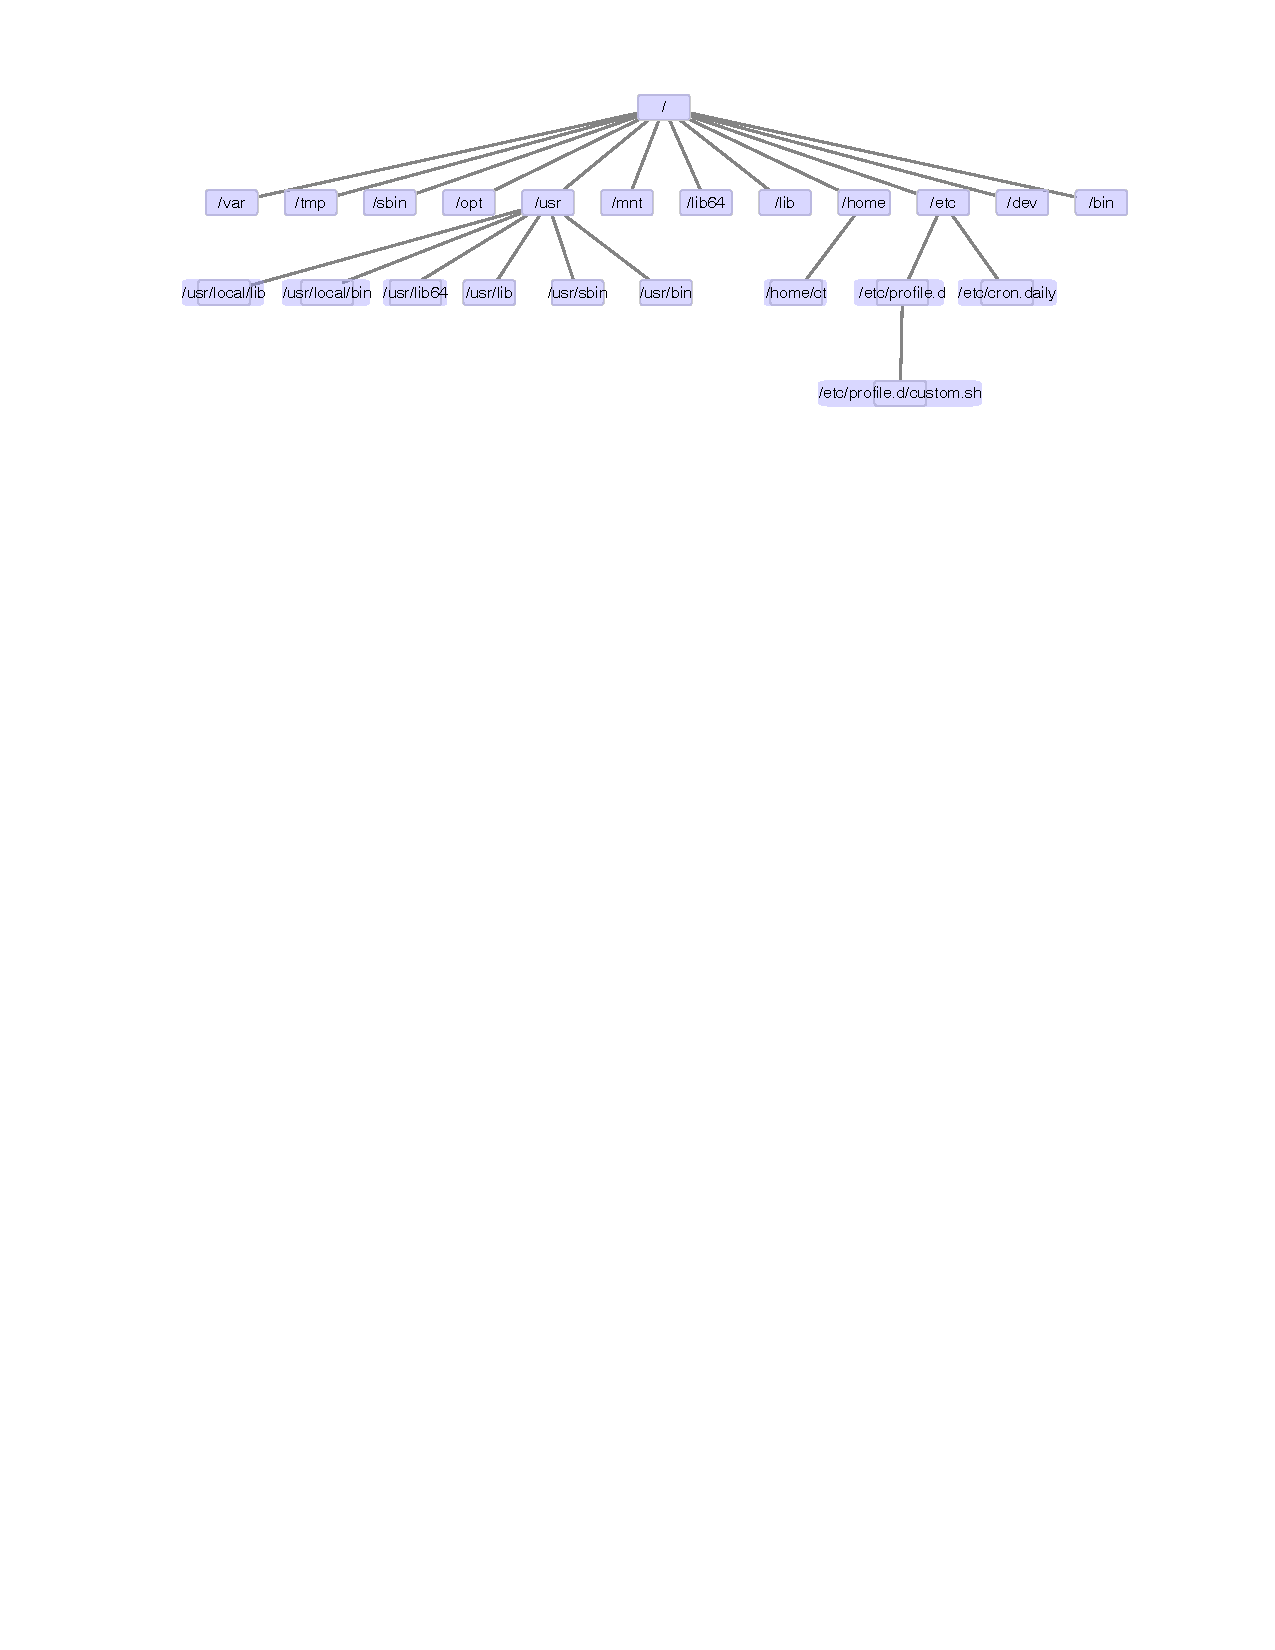
\includegraphics[width=0.95\linewidth,height=0.7\textheight,keepaspectratio=true]{image/Linux_dir} 

}

\caption{Linux目录层级结构。}\label{fig:unnamed-chunk-5}
\end{figure}

\begin{table}

\caption{\label{tab:unnamed-chunk-7}Linux下目录简介}
\centering
\begin{tabular}[t]{ll}
\toprule
Path & Description\\
\midrule
/ & 根目录\\
/bin & 常用软件如ls, mkdir, top等的存放地\\
/dev & 硬件相关\\
/etc & 存放系统管理和配置相关文件\\
/etc/cron* & 与定时任务相关的文件夹,可执行程序放置到对应文件夹就可以定时执行\\
\addlinespace
/etc/profile.d & 目录下存放Bash相关的配置文件,相当于全局的.bashrc\\
/etc/profile.d/custom.sh & 我在配置全局环境时,一般写入这个文件;如果不存在,可以新建。\\
/home & 家目录,默认新建用户的个人家目录都在此文件夹下\\
/home/ct & 用户名为ct的用户的家目录\\
/lib -> usr/lib & 存放动态库的目录 (library),安装软件时碰到依赖的动态库一般存储于此\\
\addlinespace
/lib64 -> usr/lib64 & 64位软件动态库,-> 表示软连接,等同于快捷方式\\
/mnt & 文件系统挂载,一般插入U盘会显示在这。\\
/opt & 部分额外安装的软件会置于此\\
/root & 根用户的家目录\\
/sbin -> usr/sbin & 根用户的管理命令\\
\addlinespace
/tmp & 临时目录,会定时清空,常用于存放中间文件\\
/usr & 存放系统应用的目录,前面有几个目录都是该目录下子目录的软链\\
/usr/bin & 大部分应用程序安装于此\\
/usr/sbin & 根用户的管理命令\\
/usr/lib & 存放动态库的目录 (library),安装软件时碰到依赖的动态库一般存储于此\\
\addlinespace
/usr/lib64 & 64位软件动态库\\
/usr/local/bin & 存放本地安装的命令\\
/usr/local/lib & 存放本地安装的库\\
/var & 存放各服务的日志文件。若装有网络服务,一般在/var/www/html下。\\
\bottomrule
\end{tabular}
\end{table}

作为一个普通用户,通常只在\texttt{/home/usr}, \texttt{/tmp}下有\textbf{可写}的权限,其它目录最多是\textbf{可读、可执行},部分目录连读的权限都没有。这种权限管理方式是Linux能成为真正多用户系统的一个原因。后面我们会讲解如何查看并修改这些权限。

\hypertarget{linux_system_hardware}{%
\subsubsection{系统配置怎样?来看看256M硬盘的服务器}\label{linux_system_hardware}}

看完目录结构了,来看一下硬盘有多大,有多少可用空间,只需要运行\texttt{df\ -h}命令。

除了看硬盘,还想看下CPU、内存、操作系统呢?

\begin{verbatim}
Hostname is localhost.localdomain,Ip address is 192.168.1.30.

The 64 bit operating system is  CentOS release 6.9 (Final), 
	
Nuclear info is 2.6.32-696.10.1.el6.x86_64.

The CPU is Intel(R) Xeon(R) CPU E9-5799 v2 @ 3.90GHz.

There are 8 physical cpu, each physical cpu has 0 cores, 0 threads.

There are 96 logical cpu.

The memory of this server is 252G.
\end{verbatim}

\hypertarget{directpry_show}{%
\subsubsection{看下目录下都有什么}\label{directpry_show}}

通常登陆后直接进入家目录,下面大部分操作也是在家目录下完成的。如果想查看当前目录下都有什么内容,输入命令 \texttt{ls},回车即可 (ls可以理解为单词list的缩写)。当前目录下什么也没有,所以没有任何输出。

如果错把\texttt{l}看成了\texttt{i},输入了\texttt{is},则会出现下面的提示\texttt{未找到命令}。如果输入的是Linux基本命令,出现这个提示,基本可以判定是命令输入错了,瞪大眼睛仔细看就是了。 \textbf{在敲完命令回车后,注意查看终端的输出,以判断是否有问题。}

当前目录下只有一个文件,看不出效果,我们可以新建几个文件和文件夹。

\hypertarget{mkdir}{%
\subsubsection{新建一个目录}\label{mkdir}}

\texttt{mkdir}是新建一个目录 (\texttt{m}a\texttt{k}e a \texttt{dir}ectory);\texttt{data}是目录的名字。
如果目录存在,则会出现提示,``无法创建已存在的目录''。这时可以使用参数\texttt{-p}忽略这个错误。

\texttt{cat}是一个命令,主要用来查看文件;在这与\texttt{\textless{}\textless{}END}连用用于读入大段数据。输入\texttt{cat\ \textless{}\textless{}END}之后,回车,会看到终端出现一个大于号,大于号后面可以输入内容,再回车,继续输入内容,直到我们输入\texttt{END} (大写的,与上面一致),输入过程结束,我们输入的内容都显示在了屏幕上。

如果我们想把这些内容写入文件,就需要使用 \texttt{command\ \textgreater{}\ filename}格式。

\texttt{\textgreater{}}是一个重定向符号,即把前面命令的输出写入到\texttt{\textgreater{}}后面的文件中。如下所示,新建了一个\texttt{Fasta}格式的文件。

\texttt{ls\ -l}列出文件的详细信息;\texttt{-l}表示命令行参数,是程序预留的一些选项,保证在不更改程序的情况下获得更灵活的操作。可使用\texttt{man\ ls}查看\texttt{ls}所有的命令行参数, \textbf{上下箭头翻页},按\texttt{q}退出查看。(man: manual, 手册)

\hypertarget{cat_file}{%
\subsubsection{访问文件}\label{cat_file}}

查看写入的文件的内容,\texttt{cat\ 文件名};需要注意的是文件所在的目录,默认是当前目录;如下面第一个命令,会提示\texttt{cat:\ test.fa:\ 没有那个文件或目录},是因为当前目录下不存在文件\texttt{test.fa}。(注意文件末尾的end)

\texttt{test.fa}在目录\texttt{data}下,可以先进入\texttt{data}目录,然后再查看文件。类比于Windows下先点开一个文件夹,再点开下面的文件。

这个例子中文件\texttt{test.fa}在当前目录的子目录\texttt{data}里面,在当前目录下直接查看\texttt{test.fa}就像在\texttt{我的电脑}里面不进入C盘,就像打开\texttt{Program\ file}文件夹。这属于\textbf{隔空打牛}的境界,不是一般人能练就的。起码Linux下不可以。

提到目录,Linux下有\textbf{绝对路径}和\textbf{相对路径}的概念。

\begin{itemize}
\item
  绝对路径:以\texttt{/}开头的路径为绝对路径,如\texttt{/home/ct}, \texttt{/usr/bin}, \texttt{/home/ct/data}等。需要注意的是\texttt{\textasciitilde{}/data}等同于\texttt{/home/ct/data}, 多数情况下可以等同于绝对路径,但在一个情况下例外,软件安装时用于\texttt{-\/-prefix}后的路径必须是\texttt{/}开头的绝对路径。
\item
  相对路径: 不以\texttt{/}和\texttt{\textasciitilde{}}开头的路径都是相对路径,如\texttt{data}表示当前目录下的data目录,等同于\texttt{./data} (\texttt{.}为当前目录), \texttt{../data}表示当前目录的上一层目录下的data目录 (\texttt{../}表示上层目录)。
\end{itemize}

\texttt{pwd} (print working directory) 获取当前工作目录。

\texttt{cd} (change dir)切换目录。若\texttt{cd}后没有指定切换到那个目录,则调回家目录。特别地,\texttt{cd\ -}表示返回到最近的\texttt{cd}操作前所在目录,相当于回撤到上一个工作目录。

\texttt{head}查看文件最开始的几行,默认为10行,可使用\texttt{-n\ 6}指定查看前6行。

另外\texttt{less}和\texttt{more}也可以用来查看文件,尤其是文件内容特别多的时候。

\hypertarget{com_parameter_help}{%
\subsubsection{查看帮助,获取可用命令行参数}\label{com_parameter_help}}

前面使用的命令,有几个用到了参数如\texttt{ls\ -l}, \texttt{head\ -n\ 6}等,需要注意的是命令跟参数之间要有\textbf{空格}。

终端运行\texttt{man\ ls}可以查看\texttt{ls}所有可用的参数,上下箭头翻页,按\texttt{q}退出查看。(man: manual, 手册)

\hypertarget{first_summary}{%
\subsubsection{小结}\label{first_summary}}

\begin{enumerate}
\def\labelenumi{\arabic{enumi}.}
\item
  Linux是多用户操作系统。这一点可以从我们每个人能同时登录到同一台Linux电脑各自进行操作而不相互干扰可以体会出来。大家可以尝试下是否可以看到其它人家目录下的东西。我们后期在\textbf{权限管理}部分会涉及如何开放或限制自己的文件被他人访问。
\item
  Linux下所有目录都在\textbf{根目录}下。根目录某种程度上可类比于Windows的我的电脑,第一级子目录类比于\texttt{C盘},\texttt{D盘}等 (等我们熟练了,就忘记这个拙劣的类比吧)。
\item
  使用\texttt{mkdir}新建目录,\texttt{cd}切换目录,\texttt{pwd}获取当前工作目录,\texttt{ls}查看目录下的内容, \texttt{cat}查看文件,\texttt{man\ ls}查看ls命令的使用。
\item
  访问一个文件需要指定这个文件的路径,当前目录下的文件可省略其路径\texttt{./},其它目录下则需要指定全路径 (可以是相对路径,也可以是绝对路径)。
\end{enumerate}

\hypertarget{first_exercise}{%
\subsubsection{做个小测试}\label{first_exercise}}

\begin{enumerate}
\def\labelenumi{\arabic{enumi}.}
\tightlist
\item
  在家目录下新建文件夹\texttt{bin}和\texttt{soft}。
\item
  在\texttt{bin}和\texttt{soft}目录下各自新建一个文件,名字都是\texttt{README}。
\item
  在\texttt{bin/README}文件中写入内容:This folder is used to save executable files。
\item
  在\texttt{soft/README}文件中写入内容:This folder is used to save software source files。
\item
  查看两个\texttt{README}文件的大小。
\end{enumerate}

\hypertarget{fileoperation}{%
\subsection{Linux下文件操作}\label{fileoperation}}

\hypertarget{tac_rev}{%
\subsubsection{文件按行翻转和按列翻转}\label{tac_rev}}

两个有意思的命令,\texttt{tac}: 文件翻转,第一行变为最后一行,第二行变为倒数第二行;\texttt{rev}每列反转,第一个字符变为最后一个字符,第二个字符变为倒数第二个字符。

\hypertarget{new_file}{%
\subsubsection{新建文件的n种方式}\label{new_file}}

\texttt{nano}类似于Windows下记事本的功能,\texttt{nano\ filename}就可以新建一个文件,并在里面写内容;\texttt{ctrl+x}退出,根据提示按\texttt{Y}保存。

\texttt{vim} 功能更强大的文本编辑器。\texttt{vim\ filename}就可以新建一个文件, 敲击键盘字母\texttt{i},进入写作模式。写完后,敲击键盘\texttt{Esc}, 退出写作模式,然后输入\texttt{:w} (会显示在屏幕左下角),回车保存。\texttt{vim}的常用方法,后面会有单独介绍。

\hypertarget{file_cp_mv_rename_link}{%
\subsubsection{文件拷贝、移动、重命名、软链}\label{file_cp_mv_rename_link}}

常用的文件操作有移动文件到另一个文件夹、复制文件到另一个文件夹、文件重命名等。

\texttt{cp} (copy): 拷贝文件或文件夹 (\texttt{cp\ -r} 拷贝文件夹时的参数,递归拷贝).

\texttt{cp\ source1\ source2\ ...\ target\_dir} 将一个或多个源文件或者目录复制到已经存在的目标目录。

\texttt{cp}常用参数

\begin{quote}
-r: 递归拷贝
\end{quote}

\begin{quote}
-f: 强制覆盖
\end{quote}

\begin{quote}
-i: 覆盖前先询问
\end{quote}

\begin{quote}
-p: 保留文件或目录的属性,主要是时间戳
\end{quote}

\begin{quote}
-b: 备份复制,若目标文件存在,先备份之前的,再把新的覆盖过去
\end{quote}

\begin{quote}
-u: 更新复制,若源文件和目标文件都存在,只在源文件的修改时间比较新时才复制
\end{quote}

\texttt{mv} (move): 移动文件或文件夹

\texttt{mv\ source\ target}, 常用参数有

\begin{quote}
-f: 强制覆盖
\end{quote}

\begin{quote}
-i: 覆盖前询问
\end{quote}

\begin{quote}
-u: 更新移动
\end{quote}

\texttt{rename}: 文件重命名 (常用于批量重命名,不同的系统可能用法略有不同,使用前先\texttt{man\ rename}查看使用方法)

\texttt{ln} (link): 给文件建立快捷方式 (\texttt{ln\ -s\ source\_file\ target} 创建软连接)。

在建立软连接时,原文件要使用全路径。全路径指以\texttt{/}开头的路径。如果希望软链可以让不同的用户访问,不要使用\texttt{\textasciitilde{}}。

建立软连接,是为了在不增加硬盘存储的情况下,简化文件访问方式的一个办法。把其它文件夹下的文件链接到当前目录,使用时只需要写文件的名字就可以了,不需要再写长串的目录了。

\texttt{ln}命令常用参数

\begin{quote}
-s: 软连接
\end{quote}

\begin{quote}
-f: 强制创建
\end{quote}

\texttt{../}: 表示上一层目录;\texttt{../../}: 表示上面两层目录

\texttt{pwd} (print current/working directory): 输出当前所在的目录

\texttt{\textbackslash{}\textasciigrave{}\textasciigrave{}为键盘}Esc\texttt{下第一个按键\ (与家目录}\textasciitilde`符号同一个键),写在反引号内的命令会被运行,运行结果会放置在反引号所在的位置

使用全路径名,尤其使用家目录 \texttt{\textasciitilde{}} 符号时,只限操作用户自身有效。另外不同用户之间建立软连接,需要考虑\textbf{访问权限}问题,任意一层目录都需要可读权限 (目录的可读为\texttt{rx}都有)。

复制、移动或创建软连接时,如果目标已存在,除了使用\texttt{-f}强制覆盖外,还可以使用\texttt{rm}命令删除。

\texttt{rm}可以删除一个或多个文件和目录,也可以递归删除所有子目录,使用时一定要慎重。\texttt{rm}命令删除的文件很难恢复。

\texttt{rm\ -rf\ *}: 可以删除当前目录下所有文件和文件夹,慎用。

\texttt{rm}命令常见参数:

\begin{quote}
-f:强制删除
\end{quote}

\begin{quote}
-i: 删除前询问是否删除
\end{quote}

\begin{quote}
-r: 递归删除
\end{quote}

\hypertarget{linux_abnormal}{%
\subsubsection{Linux下命令的一些突发事故}\label{linux_abnormal}}

\textbf{命令不全}:在命令没有输入完 (引号或括号没有配对),就不小心按下了\texttt{Enter}键,终端会提示出一个\texttt{\textgreater{}}代表命令不完整,这是可以继续输入,也可以\texttt{ctrl+c}终止输入,重新再来。(下面sed命令使用时,还有另外一种命令不全的问题)

\textbf{文件名输入错误}: 多一个字母、少一个字母、大小写问题

\textbf{所在目录不对}: 访问的文件不存在于当前目录,而又没有提供绝对路径, 或软连接失效

\hypertarget{file_op_gzip_wc}{%
\subsubsection{了解和操作你的文件}\label{file_op_gzip_wc}}

常用的文件内容操作有文件压缩解压缩、文件大小行数统计、文件内容查询等。

\texttt{gzip}: 压缩文件; \texttt{gunzip}: 解压缩文件

\texttt{wc} (word count): 一般使用\texttt{wc\ -l}获取文件的行数。

获取文件中包含大于号 (\texttt{\textgreater{}})的行, \texttt{grep} (print lines matching a pattern,对每一行进行模式匹配)。

\texttt{grep}的用法很多,支持正则表达式匹配,这个后面我们会详细讲解。

替换文件中的字符: \texttt{sed}是一个功能强大的文件内容编辑工具,常用于替换、取得行号等操作。现在先有个认识,后面会详细介绍。

\texttt{\textbar{}} 为管道符,在相邻命令之间传递数据流,表示把上一个命令的输出作为下一个命令的输入。

另外一个方式,去除\texttt{HAHA},使用\texttt{cut}命令。cut更适合于矩阵操作,去除其中的一列或者多列。但在处理FASTA格式文件时有这么一个妙用。FASTA文件中序列里面是没有任何符号的,而如果名字比较长,则可以指定相应分隔符就行\texttt{cut},这样既处理了名字,又保留了序列。

\texttt{-f}: 指定取出哪一列,使用方法为\texttt{-f\ 2} (取出第2列),\texttt{-f\ 2-5} (取出第2-5列),\texttt{-f\ 2,5} (取出第2和第5列)。\textbf{注意不同符号之间的区别。}

\texttt{-d}: 设定分隔符, 默认为TAB键。如果某一行没有指定的分隔符,整行都为第一列。

\hypertarget{second_exercise}{%
\subsubsection{小结和练习}\label{second_exercise}}

\begin{enumerate}
\def\labelenumi{\arabic{enumi}.}
\tightlist
\item
  Linux下文件拷贝、移动、重命名、软连接、压缩、替换等操作。
\item
  Linux下常见问题

  \begin{itemize}
  \tightlist
  \item
    \texttt{ehbio2.fa:\ 没有那个文件或目录}:这个错误通常由什么引起,应该怎么解决?
  \item
    若文件\texttt{a}存在,运行\texttt{ln\ a\ data/b}能否成功给\texttt{a}建立软连接?
  \item
    \texttt{grep\ \textquotesingle{}\textgreater{}\ ehbio.fa}的输出是什么?
  \end{itemize}
\item
  若目标文件存在时,再运行\texttt{cp}, \texttt{mv}或\texttt{ln}会有什么提示?
\item
  计算某一个Fasta序列中序列的个数。
\end{enumerate}

\hypertarget{shortcut}{%
\subsection{Linux终端常用快捷操作}\label{shortcut}}

\begin{itemize}
\item
  命令或文件名自动补全:在输入命令或文件名的前几个字母后,按\texttt{Tab}键,系统会自动补全或提示补全
\item
  上下箭头:使用上下箭头可以回溯之前的命令,增加命令的重用,减少输入工作量
\item
  \texttt{!}加之前输入过的命令的前几个字母,快速获取前面的命令
\item
  \texttt{ctrl+a}回到命令的行首,\texttt{ctrl+e}到命令行尾,(\texttt{home}和\texttt{end}也有类似功能),用于修改命令或注释掉命令
\item
  \texttt{!!} 表示上一条命令。
\item
  替换上一个命令中的字符,再运行一遍命令,用于需要对多个文件执行同样的命令,又不想写循环的情况
\end{itemize}

\hypertarget{stdinoutpipe}{%
\subsection{Linux下的标准输入、输出、重定向、管道}\label{stdinoutpipe}}

在Linux系统中,有4个特殊的符号,\texttt{\textless{}}, \texttt{\textgreater{}}, \texttt{\textbar{}}, \texttt{-},在我们处理输入和输出时存在重要但具有迷惑性的作用。

默认Linux的命令的结果都是输出到标准输出,错误信息 (比如命令未找到或文件格式识别错误等) 输出到标准错误,而标准输出和标准错误默认都会显示到屏幕上。

\texttt{\textgreater{}}表示重定向标准输出,\texttt{\textgreater{}\ filename}就是把标准输出存储到文件filename里面。标准错误还是会显示在屏幕上。

\texttt{2\ \textgreater{}\&1} 表示把标准错误重定向到标准输出。Linux终端用\texttt{2}表示标准错误,\texttt{1}表示标准输出。

\texttt{-} (短横线):表示标准输入,一般用于1个程序需要多个输入的时候。

\texttt{\textless{}} 标准输入,后面可以跟可以产生输出的命令,一般用于1个程序需要多个输入的时候。相比\texttt{-}适用范围更广。

\texttt{\textbar{}}管道符,表示把前一个命令的输出作为后一个命令的输入,前面也有一些展示例子。用于数据在不同的命令之间传输,用途是减少硬盘存取损耗。

下面我们通过一个程序\texttt{stdout\_error.sh}来解释上面的文字 (Bash脚本写作,后面会有专门介绍),内容如下

运行这个脚本

下面看管道符和标准输入的使用。

管道符的更多应用

\hypertarget{filecontent}{%
\subsection{Linux文件内容操作}\label{filecontent}}

\hypertarget{generate_file_seq}{%
\subsubsection{命令组合生成文件}\label{generate_file_seq}}

\texttt{seq}: 产生一系列的数字; \texttt{man\ seq}查看其具体使用。我们这使用\texttt{seq}产生下游分析所用到的输入文件。

\hypertarget{sort_par}{%
\subsubsection{文件排序原来有暗仓}\label{sort_par}}

\texttt{sort}: 排序,默认按字符编码排序。如果想按数字大小排序,需添加\texttt{-n}参数。

\texttt{sort}常用参数

\begin{quote}
-n: 数值排序
\end{quote}

\begin{quote}
-h: 人类刻度的数值排序 (2K 1G等)
\end{quote}

\begin{quote}
-r: reverse, 逆序
\end{quote}

\begin{quote}
-c: check, 不排序,查看文件是否已排序好
\end{quote}

\begin{quote}
-k: 指定使用哪列或哪几列排序
\end{quote}

\begin{quote}
-m: 合并已经排序好的文件
\end{quote}

\begin{quote}
-S: 缓冲区大小,用于排序大文件时的分割排序中每次分割的文件大小
\end{quote}

\begin{quote}
-u: 重复行只保留一次
\end{quote}

\texttt{sort\ -u}: 去除重复的行,等同于\texttt{sort\ \textbar{}\ uniq}。

\texttt{sort\ file\ \textbar{}\ uniq\ -d}: 获得重复的行。(\texttt{d}=\texttt{duplication})

\texttt{sort\ file\ \textbar{}\ uniq\ -c}: 获得每行重复的次数。

整理下\texttt{uniq\ -c}的结果,使得原始行在前,每行的计数在后。

\texttt{awk}是一个强大的文本处理工具,其处理数据模式为按行处理。每次读入一行,进行操作。

\begin{itemize}
\tightlist
\item
  \texttt{OFS}: 输出文件的列分隔符 (output file column separtor);
\item
  \texttt{FS}为输入文件的列分隔符 (默认为空白字符);
\item
  \texttt{awk}中的列从第1到n列,分别记录为\texttt{\$1}, \texttt{\$2} \ldots{} \texttt{\$n};
\item
  \texttt{BEGIN}表示在文件读取前先设置基本参数;与之相对应的是\texttt{END},只文件读取完成之后进行操作;
\item
  不以\texttt{BEGIN}, \texttt{END}开头的\texttt{\{\}}就是文件读取、处理的部分。每次对一行进行处理。后面会详细讲解。
\end{itemize}

对两列文件,按照第二列进行排序, \texttt{sort\ -k2,2n}。

两个暗仓:

\begin{enumerate}
\def\labelenumi{\arabic{enumi}.}
\tightlist
\item
  sort默认文件列分隔符是所有空字符,若同时存在和会有非预期结果。
\item
  \texttt{sort\ -t\ \textquotesingle{}\textbackslash{}t\textquotesingle{}}是错误用法,TAB键的正确输入方式是:先按\textless ctrl+v\textgreater 再按。
\end{enumerate}

\hypertarget{ux5b9eux6218fastaux5e8fux5217ux63d0ux53d6-fasta_extract}{%
\subsubsection{实战FASTA序列提取 {[}\#fasta\_extract\}}\label{ux5b9eux6218fastaux5e8fux5217ux63d0ux53d6-fasta_extract}}

生成单行序列FASTA文件,提取特定基因的序列,最简单的是使用\texttt{grep}命令。

\texttt{grep}在前面也提到过,以后还会经常提到,主要用途是匹配文件中的字符串,以此为基础,进行一系列的操作。如果会使用正则表达式,将会非常强大。正则表达式版本很多,几乎每种语言都有自己的规则,后面会详细展开。

多行FASTA序列提取要麻烦些,一个办法就是转成单行序列,用上面的方式处理。

\texttt{sed}和\texttt{tr}都为最常用的字符替换工具。

\begin{quote}
\texttt{\textgreater{}}SOX2 ACGAGGGACGCATCGGACGACTGCAGGACTGTC ACGAGGGACGCATCGGACGACTGCAGGACTGTC ACGAGGGACGCATCGGACGACTGCAGGAC \textgreater POU5F1 CGGAAGGTAGTCGTCAGTGCAGCGAGTCCGT CGGAAGGTAGTCGTCAGTGCAGCGAGTCC \textgreater NANOG ACGAGGGACGCATCGGACGACTGCAGGACTGTC ACGAGGGACGCATCGGACGACTGCAGG ACGAGGGACGCATCGGACGACTGCAGGACTGTC ACGAGGGACGCATCGGACGACTGCAGGACTGT
\end{quote}

\begin{verbatim}
# >号前面加换行符
ct@ehbio:~$ cat test.fasta | tr '\n' '\t' | sed 's/\t>/\n>/g'
\end{verbatim}

\begin{quote}
\texttt{\textgreater{}}SOX2 ACGAGGGACGCATCGGACGACTGCAGGACTGTC ACGAGGGACGCATCGGACGACTGCAGGACTGTC ACGAGGGACGCATCGGACGACTGCAGGAC
\end{quote}

\begin{quote}
\texttt{\textgreater{}}POU5F1 CGGAAGGTAGTCGTCAGTGCAGCGAGTCCGT CGGAAGGTAGTCGTCAGTGCAGCGAGTCC
\end{quote}

\begin{quote}
\texttt{\textgreater{}}NANOG ACGAGGGACGCATCGGACGACTGCAGGACTGTC ACGAGGGACGCATCGGACGACTGCAGG ACGAGGGACGCATCGGACGACTGCAGGACTGTC ACGAGGGACGCATCGGACGACTGCAGGACTGT
\end{quote}

\begin{verbatim}
# 先把第一个TAB键变为换行符,实现序列名字和序列的分离
# 再去掉序列中所有的TAB键
ct@ehbio:~$ cat test.fasta | tr '\n' '\t' | sed 's/\t>/\n>/g' \
		| sed 's/\t/\n/' | sed 's/\t//g' >test.oneline.fa
\end{verbatim}

\begin{quote}
\texttt{\textgreater{}}SOX2
\end{quote}

\begin{quote}
ACGAGGGACGCATCGGACGACTGCAGGACTGTCACGAGGGACGCATCGGACGACTGCAGGACTGTCACGAGGGACGCATCGGACGACTGCAGGAC
\end{quote}

\begin{quote}
\texttt{\textgreater{}}POU5F1
\end{quote}

\begin{quote}
CGGAAGGTAGTCGTCAGTGCAGCGAGTCCGTCGGAAGGTAGTCGTCAGTGCAGCGAGTCC
\end{quote}

\begin{quote}
\texttt{\textgreater{}}NANOG
\end{quote}

\begin{quote}
ACGAGGGACGCATCGGACGACTGCAGGACTGTCACGAGGGACGCATCGGACGACTGCAGGACGAGGGACGCATCGGACGACTGCAGGACTGTCACGAGGGACGCATCGGACGACTGCAGGACTGT
\end{quote}

或者简单点,直接用前面的\texttt{awk}略微做下修改。

\hypertarget{linux_search}{%
\subsection{Linux下的查找命令 - 文件哪里跑}\label{linux_search}}

查找是我们每天都在做的事情,早上醒来找下手机,出门之前查下公交,坐下之后查下资料,分析数据查下模式。

查找文件,查找信息,查找错误是应用起来更为具体的一些工作,而Linux命令行为我们提供了很多快捷强大的查找方式。

\hypertarget{seach_cmmand}{%
\subsubsection{命令/可执行程序查找 - 定位脚本的位置}\label{seach_cmmand}}

\texttt{whereis\ program\_name}: 会在系统默认安装目录(一般是有root权限时默认安装的软件)和\texttt{\$PATH}, \texttt{\$MANPATH}指定的目录中查找二进制文件、源码、文档中包含给定查询关键词的文件。(默认目录有 \texttt{/bin}, \texttt{/sbin}, \texttt{/usr/bin}, \texttt{/usr/lib}, \texttt{/usr/local/man}等类似路径)

\texttt{which\ program\_name}: 会给出所有在\href{http://mp.weixin.qq.com/s/poFpNHQgHDr0qr2wqfVNdw}{环境变量}中的程序的路径,一来方便知道运行的程序在哪,二来方便修改。比如\href{https://mp.weixin.qq.com/s/_9LKs6t6rcjzokF_0gneSA}{vim `which sp\_pheatmap.sh`}就可以直接修改绘制热图的脚本,\texttt{cp\ \textbackslash{}}which sp\_pheatmap.sh` .`可以直接把源码拷贝到当前目录,省去了写全路径的麻烦。

如果运行\texttt{which\ bwa},系统返回是 \texttt{/usr/bin/which:\ no\ bwa\ in\ (/home/usr/bin:/bin)}则说明bwa没有安装或安装后没有放置在环境变量中,不可以直接写名字调用。

\hypertarget{locate}{%
\subsubsection{locate普通文件快速定位}\label{locate}}

\texttt{locate}是快速查找定位文件的好方法,但其依赖于\texttt{updatedb}建立的索引。而\texttt{updatedb}一般是每天运行一次,所以当天新建的文件是索引不到的。如果有根用户权限,可以手动运行\texttt{updatedb}做个更新,然后再\texttt{locate\ bwa}。(个人用户也可以构建自己的\texttt{updatedb}, 使用\texttt{locate}在局部环境中查找。)

\begin{verbatim}
ct@ehbio:~$ locate R.sys
/soft/R.sys
\end{verbatim}

\hypertarget{find}{%
\subsubsection{find让文件无处可逃 find}\label{find}}

\texttt{find\ /\ -name\ bwa}可以搜索根目录下所有名字为bwa的文件

运行上面的命令时会输出很多\texttt{Permission\ denied},是因为 作为普通用户,无权限访问一些目录,因此会有提示输出,可以使用\texttt{find\ /\ -name\ bwa\ 2\textgreater{}/dev/null}重定向标准错误到空设备,报错信息就被扔掉了,还不影响正常输出。

\begin{verbatim}
ct@ehbio:~$ find / -name R 2>/dev/null
/usr/bin/R
/usr/lib/rstudio-server/R
/usr/share/groff/1.22.2/font/devascii/R
/usr/share/groff/1.22.2/font/devhtml/R
/usr/share/groff/1.22.2/font/devlatin1/R
/usr/share/groff/1.22.2/font/devutf8/R
/usr/local/bin/R
/usr/local/lib64/R
/usr/local/lib64/R/share/R
/usr/local/lib64/R/bin/R
\end{verbatim}

\hypertarget{find_by_time}{%
\paragraph{按时间查找}\label{find_by_time}}

我们开发的在线画图网站 (\href{http://mp.weixin.qq.com/s/pTHHqxuf0y1MCCCBaZjt9A}{www.ehbio.com/ImageGP}),为了追踪每天用户使用时碰到了什么问题,需要每天定时去查看日志。

这个命令\texttt{find\ .\ -name\ *.log\ -mmin\ \ -60}可以查看当前目录下(包括所有子目录)一小时内修改的日志文件。再配合\texttt{head}就可以查看每个日志文件的内容,以方便查看使用过程中出现了哪些错误,如何增加提示或修改画图程序。

正是有了这个利器,前台的错误提示中才出现了这么一句话,\textbf{如果您核对后数据和参数没问题,请过1天再进行尝试。若是程序问题,我们通常会在1天内修复。}

当然后台数据都是用时间戳存储的,而且若无报错,数据会直接删掉,有报错的才会保留日志,不会泄露用户信息,这点大家不用担心。

现在画图网站越来越稳定,出现的问题越来越少,前台提示也越来越完善,希望大家使用时多看下提示,查看日志的频率也少了,就使用\texttt{find\ .\ -name\ *.log\ -mtime\ -1}查看从现在起24小时内的日志了。

这个也有个问题,每次查看的时间可能不一致,会漏查或有重叠,于是在某次查看完日志后,使用\texttt{touch\ check}在当前目录下新建了个空文件。以后再查日志文件时,只要使用\texttt{find\ .\ -name\ *.log\ -newer\ check}就可以获得所有上次查看过之后的新日志。每次查看完之后,都做个书签,就方便多了。

慢慢发现有空日志文件, 使用\texttt{find\ .\ -name\ *.log\ -newer\ check\ -size\ +0}过滤掉, 只保留大小大于0的文件。就这样在小伙伴聪明勤奋地维持下,我们绘图网站为\textbf{7万}多用户提供了近\textbf{100万}次服务 (\href{https://mp.weixin.qq.com/s/ekTLcXSJh14Bm3PtVc9Mpg}{画图手册 \textbar{} ImageGP:今天你``plot''了吗?})。

\hypertarget{ux6309ux7c7bux578bux548cux5927ux5c0fux67e5ux627e-find_by_type_size}{%
\paragraph{按类型和大小查找 \{\$find\_by\_type\_size\}}\label{ux6309ux7c7bux578bux548cux5927ux5c0fux67e5ux627e-find_by_type_size}}

如果我想得到当前目录下所有\texttt{png}和\texttt{jpg}照片呢?

使用 \texttt{find\ .\ \textbackslash{}(\ -name\ "*.png"\ -o\ -name\ "*.jpg"\ \textbackslash{})\ \textbar{}\ less}

或 \texttt{find\ .\ -regex\ ".*\textbackslash{}(\textbackslash{}.png\textbackslash{}\textbar{}\textbackslash{}.jpg\textbackslash{})\$"}

\texttt{find\ .\ -type\ f\ -size\ +100G}可以获取大小超过100G的文件。

\hypertarget{find_maxdepth}{%
\paragraph{限制查找深度}\label{find_maxdepth}}

只看当前目录2层子目录内的文件\texttt{find\ .\ -maxdepth\ 2\ -name\ *.log}。

查看不是\texttt{log}结尾的文件\texttt{find\ .\ -not\ -name\ *.log}。还有更多组合操作,详见find文档。

\hypertarget{grep_file}{%
\subsubsection{按文件内容查找 grep}\label{grep_file}}

find可以查找包含某句话的文件吗? 还是拿我们的日志说事吧,\texttt{find\ .\ -name\ *.log\ -exec\ grep\ -l\ \textquotesingle{}Error\textquotesingle{}\ \{\}\ \textbackslash{};}就可以返回所有包含\texttt{Error}单词的文件名。

\texttt{find\ .\ -name\ *.log\ \textbar{}\ xargs\ grep\ -l\ \textquotesingle{}Error\textquotesingle{}}也可以。

\texttt{grep\ -rl\ \textquotesingle{}Error\textquotesingle{}\ *}也可以,不加\texttt{-l}还可以顺便返回匹配的行。

\textbf{匹配行的前后行}

\texttt{grep\ -A\ 5\ -B\ 1\ \textquotesingle{}Bioinfo\textquotesingle{}\ ehbio.log}可以查看匹配行的前1行(B, before)和后5行(A, after)。

\textbf{匹配次数}

\texttt{grep\ -c\ \textquotesingle{}Bioinfo\textquotesingle{}\ ehbio.log}可以统计包含Bioinfo的行数

\texttt{grep\ -ci\ \textquotesingle{}Bioinfo\textquotesingle{}\ ehbio.log}则会在匹配时忽略大小写。

统计FASTA序列中的序列数 \texttt{grep\ \textquotesingle{}\^{}\textgreater{}\textquotesingle{}\ ehbio.fa}

统计FASTQ序列中的序列数 \texttt{grep\ \textquotesingle{}\^{}+\$\textquotesingle{}\ ehbio.fq}。(\^{}表示以什么开头,\$表示以什么结尾)。

\textbf{获取未匹配行}

\texttt{grep\ -v\ \textquotesingle{}Bioinfo\textquotesingle{}\ ehbio.log},读读手册(\texttt{man\ grep}),可以看到更多参数使用。

\textbf{序列提取}

假设有个基因列表文件 (ID),有个单行序列的FASTA文件 (ehbio.fa), 运行如下命令\texttt{grep\ -A\ 1\ -Fw\ -f\ id\ ehbio.fa\ \textbar{}\ grep\ -v\ -\/-\ \textquotesingle{}-\/-\textquotesingle{}}就可以批量提取序列了。

\texttt{-f\ id}表示把id文件中的每一行作为一个匹配模式。\texttt{-F}表示匹配模式作为原始字符串,而非正则表达式,这是以防有特殊字符被解析。\texttt{-w}则表示作为一个单词匹配,即假如id中有\texttt{Sox2},那么它会匹配\texttt{Sox2},也会匹配\texttt{Sox21};如果加了\texttt{-w},则不会匹配\texttt{Sox21}。

更好的序列批量提取见 \href{http://mp.weixin.qq.com/s/R1OHRhZoDJuAdyVdJr2xHg}{awk的使用}。

\textbf{模式匹配}

grep强大的功能是支持正则匹配,默认使用基本正则表达式,\texttt{-E}使用扩展的正则表达式,\texttt{-P}使用perl格式的正则表达式。

比如想去掉文件中所有的空行\texttt{grep\ -v\ \textquotesingle{}\^{}\$\textquotesingle{}\ ehbio.fa\ \textgreater{}ehbio.clean.fa};

从公众号文章中搜索跟文章写作相关的文章 \texttt{grep\ \textquotesingle{}writ.*\textquotesingle{}\ *.md} (可以匹配write, writing等字);

正则表达式就比较多了,具体可以看\url{http://mp.weixin.qq.com/s/4lUiZ60-aXLilRk9--iQhA}。

\hypertarget{grep_faster}{%
\subsection{一句话加速grep近30倍}\label{grep_faster}}

最近做一个项目,需要从表达矩阵中提取单个特定基因的表达值。最开始时文件比较小,使用\texttt{awk}单个读取处理也很快,但后来数据多了,从一个\texttt{1.2\ G}的文件中提取单个基因的表达需要\texttt{30\ s},用\texttt{grep}来写需要\texttt{25\ S},这在平时写程序是可以接受的,但在网站上是接受不了的。所以就想着如何优化一下。

探索下来优化也很简单,把\texttt{grep}换为\texttt{LC\_ALL=C\ grep}再加其它参数速度就快了近\textbf{30}倍,把时间控制在\texttt{1\ s}左右。

下面是整个探索过程 (写这篇总结文章是在早晨,服务器不繁忙,所以下面的示例中只能看出来快了\texttt{5}倍左右。这也表明不加\texttt{LC\_All=C}时\texttt{grep}受服务器负载影响较大,加了之后则几乎不受影响。)

\hypertarget{grep_single_gene}{%
\subsubsection{获取单基因表达量}\label{grep_single_gene}}

查看下文件大小

\begin{verbatim}
ls -sh 334d41a7-e34a-4bab-841c-eb07bd84513f.txt

# 1.2G 334d41a7-e34a-4bab-841c-eb07bd84513f.txt
\end{verbatim}

查看下文件内容

\begin{verbatim}
head 334d41a7-e34a-4bab-841c-eb07bd84513f.txt | cut -f 1,2

# Rnu2-1	-0.52
# Tmsb4Xp6	11.81
# S100A14	1.99
# Krt17	1.26
# Aldh1A1	6.92
# Fxyd3	0.56
# Rnu2-2P	0.35
# Rarres1	6.03
# Rnvu1-7	9.53
# Lcn2	3.44
\end{verbatim}

假设基因名字大小写一致时使用\texttt{awk}提取其表达信息,用时\texttt{14\ s}。

\begin{verbatim}
time awk '{if($1=="Tmsb4Xp6") print $2;}' 334d41a7-e34a-4bab-841c-eb07bd84513f.txt >1

real	0m14.569s
user	0m12.943s
sys	0m0.626s
\end{verbatim}

实际上大小写可能不一致而需要转换,耗时\texttt{17\ s}。

\begin{verbatim}
time awk '{if(tolower($1)=="tmsb4xp6") print $2;}' 334d41a7-e34a-4bab-841c-eb07bd84513f.txt >2

real	0m17.638s
user	0m17.031s
sys	0m0.595s
\end{verbatim}

采用\texttt{grep}命令提取 (\texttt{-i}忽略大小写),用时\texttt{5\ s}。

\begin{verbatim}
time cat 334d41a7-e34a-4bab-841c-eb07bd84513f.txt | grep -i 'Tmsb4Xp6' >4

real	0m5.454s
user	0m5.134s
sys	0m1.272s
\end{verbatim}

上面的\texttt{grep}是全句匹配,想着加上\texttt{\^{}}匹配行首是否会减少匹配量,速度能快一些,效果不明显,用时\texttt{4\ s}。

\begin{verbatim}
time cat 334d41a7-e34a-4bab-841c-eb07bd84513f.txt | grep -iP '^Tmsb4Xp6' >5

real	0m4.262s
user	0m3.984s
sys	0m1.233s
\end{verbatim}

\texttt{grep}是处理匹配关系,获得的是包含关键词但不一定全等于关键词,加一个\texttt{-w}参数,匹配更精确些,耗时\texttt{6.7\ s}。

\begin{verbatim}
time cat 334d41a7-e34a-4bab-841c-eb07bd84513f.txt | grep -iPw '^Tmsb4Xp6' >6

real	0m6.723s
user	0m6.390s
sys	0m1.348s
\end{verbatim}

从上面来看,采用正则限定并不能提速,还是采用固定字符串方式提取,速度也差不多,耗时\texttt{5\ s}。(\texttt{fgrep}等同于\texttt{grep\ -F})

\begin{verbatim}
time cat 334d41a7-e34a-4bab-841c-eb07bd84513f.txt | fgrep -i 'Tmsb4Xp6' >7

real	0m5.496s
user	0m5.128s
sys	0m1.366s
\end{verbatim}

主角出场,加上\texttt{LC\_ALL=C}后,速度明显提升了,只需要\texttt{1\ s}时间。

\begin{verbatim}
time LC_ALL=C fgrep -i '^Tmsb4Xp6' 334d41a7-e34a-4bab-841c-eb07bd84513f.txt >8

real	0m1.027s
user	0m0.671s
sys	0m0.355s
\end{verbatim}

多次测试下来,发现添加\texttt{LC\_ALL=C}后\texttt{grep}命令快了很多,而且多次测试速度都很稳定 (不论服务器是繁忙还是空闲)。这里面的原理是涉及字符搜索空间的问题,我们操作的文件只包含字母、字符、数字,没有中文或其它复杂符号时都是适用的,具体原理和更多评估可查看文末的两篇参考链接,了解更多信息。

为了简化应用,我们可以\texttt{alias\ grep=\textquotesingle{}LC\_ALL=C\ grep\textquotesingle{}} (把这句话放到\texttt{\textasciitilde{}/.bashrc}或\texttt{\textasciitilde{}/.bahs\_profile}里面),后续再使用\texttt{grep}时就可以直接得到速度提升了。

\begin{verbatim}
time grep -F -i '^Tmsb4Xp6' 334d41a7-e34a-4bab-841c-eb07bd84513f.txt 

real	0m1.013s
user	0m0.679s
sys	0m0.334s
\end{verbatim}

\hypertarget{grep_multiple_gene}{%
\subsubsection{那如果获取多个基因怎么操作呢?}\label{grep_multiple_gene}}

一个方式是使用正则表达式,多个基因一起传递过去,分别匹配,耗时\texttt{4.6\ s}。

\begin{verbatim}
time cat 334d41a7-e34a-4bab-841c-eb07bd84513f.txt | LC_ALL=C grep -iP 'Tmsb4Xp6|Sox1|Sox2|Sox3'

real	0m4.654s
user	0m4.366s
sys	0m1.227s
\end{verbatim}

或者还是使用固定字符串查找模式,把所有基因每行一个写入文件\texttt{a},然后再去匹配,耗时\texttt{2.5\ s},且测试发现在基因数目少于\texttt{10}时(这是通常的应用场景),基因多少影响不大 (这也说明能用固定字符串查找时最好显示指定)。

\begin{verbatim}
time cat 334d41a7-e34a-4bab-841c-eb07bd84513f.txt | LC_ALL=C fgrep -i -f a >11

real	0m2.539s
user	0m2.191s
sys	0m1.249s
\end{verbatim}

这里还比较了另外2个号称比\texttt{grep}快的命令\texttt{ag}和\texttt{rg}在这个应用场景没体现出性能优势。

\begin{verbatim}
time cat 334d41a7-e34a-4bab-841c-eb07bd84513f.txt | LC_ALL=C ag -i '^Tmsb4Xp6|Sox1|Sox2|Sox3' >10

real	0m11.281s
user	0m9.713s
sys	0m5.326s

time cat 334d41a7-e34a-4bab-841c-eb07bd84513f.txt | rg -iF -f a >12

real	0m4.337s
user	0m3.444s
sys	0m2.787s
\end{verbatim}

\begin{itemize}
\tightlist
\item
  \url{https://www.inmotionhosting.com/support/website/speed-up-grep-searches-with-lc-all/}
\item
  \url{https://stackoverflow.com/questions/42239179/fastest-way-to-find-lines-of-a-file-from-another-larger-file-in-bash\#}
\end{itemize}

\hypertarget{top}{%
\subsection{监控程序的运行时间和资源占用}\label{top}}

\begin{enumerate}
\def\labelenumi{\arabic{enumi}.}
\tightlist
\item
  监测命令的运行时间 \texttt{time\ command}
\end{enumerate}

\begin{verbatim}
ct@ehbio:~$ time sleep 5

real	0m5.003s # 程序开始至结束的时间,包括其它进程占用的时间片和IO时间
user	0m0.001s # 进程真正执行占用CPU的时间, 
sys	0m0.002s     # 进程在内核中调用所消耗的CPU时间
user+sys是进程实际的CPU时间。如果多线程执行,这个时间可能大于Real。如果IO是瓶颈,则real会大于user+sys (单线程)。
\end{verbatim}

\begin{enumerate}
\def\labelenumi{\arabic{enumi}.}
\setcounter{enumi}{1}
\tightlist
\item
  查看正在运行的命令和其资源使用 \texttt{top}
\end{enumerate}

\begin{itemize}
\tightlist
\item
  top输出界面第一行主要信息是负载显示,分别是1分钟、5分钟、15分钟前到现在的任务队列的平均长度。
\item
  一般与CPU数目相当为好,过大系统负载超额,反应慢。
\item
  在top输出界面输入 \texttt{u}, 会提示输入用户名,以查看某个用户的进程。
\item
  重点关注的是\%MEM列,查看系统占用的内存是否超出。
\end{itemize}

\begin{verbatim}
ct@ehbio:~$ top -a #按内存排序显示

top - 09:02:11 up 224 days,  8:34,  30 users,  load average: 40, 33, 28
Tasks: 1561 total,   1 running, 1550 sleeping,   0 stopped,  10 zombie
Cpu(s):  0.6%us,  0.2%sy,  0.0%ni, 99.2%id,  0.0%wa,  0.0%hi,  0.0%si,  0.0%st
Mem:  2642768880k total, 2094619800k used, 548149080k free,   4310240k buffers
Swap: 86472700k total, 73226016k used, 13246684k free, 193383748k cached

  PID USER      PR  NI  VIRT  RES  SHR S %CPU %MEM    TIME+  COMMAND                                  
32527 ct        20   0 2631m 1.7g 1332 S  0.0  0.7 100:34.87 rsem-run-em 
29273 ct        20   0 4094m 692m 3396 S  0.0  0.3  45:18.83 java -Xmx1000m
40148 mysql     20   0 21.9g 606m 6116 S  1.3  0.2   2536:06 /usr/sbin/mysqld
31040 ct        20   0 1887m  77m 2604 S  0.3  0.0 180:43.16 [celeryd: 
\end{verbatim}

\begin{enumerate}
\def\labelenumi{\arabic{enumi}.}
\setcounter{enumi}{2}
\tightlist
\item
  查看系统进程 \texttt{ps\ auwx\ \textbar{}\ grep\ \ \textquotesingle{}process\_name\textquotesingle{}}
\end{enumerate}

\hypertarget{references}{%
\subsection{References}\label{references}}

\begin{itemize}
\tightlist
\item
  原文链接 \url{http://blog.genesino.com//2017/06/bash1/}
\item
  微信公众号 \url{http://mp.weixin.qq.com/s/yKP1Kboji9N4p2Sl1Ovj0Q}
\item
  \href{http://mp.weixin.qq.com/s/hEYU80fPf1eD5OWL3fO4Bg}{Linux-总目录}
\item
  \href{http://mp.weixin.qq.com/s/yKP1Kboji9N4p2Sl1Ovj0Q}{Linux-文件和目录}
\item
  \href{http://mp.weixin.qq.com/s/4bYMzJclf_xHpqdrlbvAdA}{Linux-文件操作}
\item
  \href{http://mp.weixin.qq.com/s/QFgINAYcQA9kYYSA28wK-Q}{Linux文件内容操作}
\item
  \href{http://mp.weixin.qq.com/s/poFpNHQgHDr0qr2wqfVNdw}{Linux-环境变量和可执行属性}
\item
  \href{http://mp.weixin.qq.com/s/zL9Mw_2ig48gHrIjKM0CMw}{Linux - 管道、标准输入输出}
\item
  \href{http://mp.weixin.qq.com/s/TNU7X2mhfVVffaJ7NRBuNA}{Linux - 命令运行监测和软件安装}
\item
  \href{http://mp.weixin.qq.com/s/cDIN4_R4nETEB5irmIGFAQ}{Linux-常见错误和快捷操作}
\item
  \href{http://mp.weixin.qq.com/s/1QaroFE7AH1pREuq-k2YAw}{Linux-文件列太多,很难识别想要的信息在哪列;别焦急,看这里。}
\item
  \href{http://mp.weixin.qq.com/s/R1OHRhZoDJuAdyVdJr2xHg}{Linux-文件排序和FASTA文件操作}
\item
  \href{http://mp.weixin.qq.com/s/HLHiWMLaWtB7SOJe_jP3mA}{Linux-应用Docker安装软件}
\item
  \href{http://mp.weixin.qq.com/s/c2cspK5b4sQScWYMBtG63g}{Linux服务器数据定期同步和备份方式}
\item
  \href{https://mp.weixin.qq.com/s/4lUiZ60-aXLilRk9--iQhA}{VIM的强大文本处理方法}
\item
  \href{http://mp.weixin.qq.com/s/A4_j8ZbyprMr1TT_wgisQQ}{Linux - Conda软件安装方法}
\item
  \href{http://mp.weixin.qq.com/s/xq0JfkHJJeHQk1acjOAJUQ}{查看服务器配置信息}
\item
  \href{http://mp.weixin.qq.com/s/cywkIeRbhkYTZvkwTeIVSA}{Linux - SED操作,awk的姊妹篇}
\item
  \href{http://mp.weixin.qq.com/s/8wD14FXt7fLDo1BjJyT0ew}{Linux - 常用和不太常用的实用awk命令}
\item
  \href{http://mp.weixin.qq.com/s/lWNp_6W_jLiogmtlk9nO2A}{Bash概论 - Linux系列教程补充篇}
\item
  \href{https://mp.weixin.qq.com/s/q3ic5WSfLdAnqIhFQX-bUQ}{原来你是这样的软连接}
\item
  \href{https://mp.weixin.qq.com/s/xWwj04h4W6yEqQLOfuQ8qA?}{一网打进Linux下那些查找命令}
\item
  \href{https://mp.weixin.qq.com/s/hyiGxm0jx6xEc90nHLN4dQ}{有了这些,文件批量重命名还需要求助其它工具吗?}
\end{itemize}

\hypertarget{softinstall}{%
\section{Linux下软件安装相关}\label{softinstall}}

视频课见 \url{http://bioinfo.ke.qq.com}。

软件安装的几个概念:环境变量、可执行属性、编译安装、Conda安装。

\hypertarget{fileattributeplusX}{%
\subsection{文件属性和可执行属性}\label{fileattributeplusX}}

\hypertarget{fileattribute}{%
\subsubsection{文件属性}\label{fileattribute}}

文件属性\texttt{rwx}中\texttt{r}表示\texttt{read} (数字表示为4)、\texttt{w}表示\texttt{write} (数字表示为2)、\texttt{x}表示执行 (数字表示为1)。三个为一组,连续出现三次(如下面命令行中所示), 第一组表示文件的所有者拥有的权限,第二组为文件所有者所在的用户组所拥有的权限,组内所有成员都具有的权限,第三组为其它用户的权限。

\texttt{chmod}可以修改文件或文件夹属性。

\hypertarget{executable}{%
\subsubsection{可执行属性}\label{executable}}

Linux下文件有一个特殊的属性即可执行属性,用来指示这个文件是一个可执行的脚本或可以运行的二进制文件。前面所提到的这些命令,都具有可执行属性。

\texttt{which}: 表示查看命令的路径。一般用于当我们想知道使用的命令来源于什么地方时,比如安装了多个R或多个python,但又分不清用的是哪个时,\texttt{which}一下,立即明了。在这儿我们用which获取的是可执行的命令所在的路径,进而查看其属性。

\texttt{chmod\ a+x\ file}: 表示给文件增加所有人(a)可执行权限 (+x)

\texttt{chmod\ u+x\ file}: 表示给文件增加所有者(u,user,)可执行权限 (+x)

\texttt{chmod\ g+x}, \texttt{chmod\ o+X}: 表示给文件增加组内人或其它人可执行权限

\texttt{chmod\ 755\ file}: 表示拥有者有可读写执行权限,其它人有可读执行权限。(\texttt{7=4+2+1}; \texttt{5=4+1})

具体使用\texttt{man\ chmod}查看其它参数使用。

如果一个文件有了可执行权限,是不是就可以执行了,我们来检测下。

事实上并非如此,输入命令,回车后,提示命令未找打,这是为什么呢?

这就涉及到\textbf{环境变量}的概念,通俗的讲,环境变量就是告诉电脑 (实际是操作系统)几个目录。这几个目录下存储又可执行文件,如前面显示的\texttt{/usr/bin}目录,大部分的系统命令都在这个目录下。

\hypertarget{PATH_path_which}{%
\subsection{PATH和path,傻傻分不清}\label{PATH_path_which}}

习惯了Windows电脑下的所见即所得,找到程序或文件双击即可运行或打开;于是我们被惯得以为电脑会像人一样聪明,给他一个名字就可以运行程序或打开文件;于是在命令行下或程序里不断碰壁,为啥这个命令不运行了呢?

我们不能太高估电脑(或操作系统),不要以为只要输入一个程序名或文件名,电脑(或操作系统)就可以满硬盘的去找这个文件在哪;这一来效率太低了,二来重名了怎么办?比如有2个文件都叫``子房.txt'',一个存储汉初三杰之张良,一个存储被子植物生长种子的器官;可能打开前我们自己也不知道要开哪个吧。

想一下,我们在Windows下寻找文件时,是不是先打开\texttt{我的电脑},然后打开\texttt{D盘},打开\texttt{学习}目录,再打开\texttt{学习计划.docx}这个文件。即便我们从来没有执行过这个计划,每天我们还是不厌其烦的一层层打开然后制定新的计划。只是,我们忽略了这个\texttt{一层层}打开。

\texttt{path}我们一般指文件的路径,也就是\texttt{一层层}打开的过程。以Linux为例:

我们要查看一个在自己家目录下的文件 \texttt{I\_am\_home.txt},那登录后,直接可见:

\begin{verbatim}
YSX@ehbio:~$ tree
.
├── I_am_home.txt
└── train
    ├── amplicon
    │   └── pipeline_amplicon.sh
    ├── metagenome
    │   └── pipeline_metagenome.sh
    ├── population_genomics
    │   └── pipeline_gatk.sh
    ├── single_cell
    │   ├── Scanpy.ipynb
    │   └── Seurat.Rmd
    └── transcriptome
        └── pipeline_salmon.sh
YSX@ehbio:~$ head I_am_home.txt
I am home!
\end{verbatim}

那如果想看\texttt{Seurat.Rmd},怎么查看?一步步找下去就对了。

\begin{verbatim}
YSX@ehbio:~$ less Seurat.Rmd
Seurat.Rmd: 没有那个文件或目录
YSX@ehbio:~$ less train/Seurat.Rmd
train/Seurat.Rmd: 没有那个文件或目录
YSX@ehbio:~$ less train/single_cell/Seurat.Rmd
\end{verbatim}

也可以一步步先做目录切换,然后再查看

\begin{verbatim}
YSX@ehbio:~$ cd train
YSX@ehbio:~/train$ cd single_cell/
YSX@ehbio:~/train/single_cell$ less Seurat.Rmd
\end{verbatim}

那如果你这时你想运行\texttt{pipeline\_metagenome.sh}快速分析宏基因组数据怎么办?

\begin{verbatim}
YSX@ehbio:~/train/single_cell$ pipeline_metagenome.sh
-bash: pipeline_metagenome.sh: 未找到命令
\end{verbatim}

\texttt{pipeline\_metagenome.sh}命令去哪儿了?上面我们都看到了,就在\texttt{metagenome}目录下,为啥电脑(操作系统)这么笨却找不到?另外为什么运行\texttt{head}就可以找到?难道有一些黑魔法在里面?

确实是有一些黑魔法的,不过我们一般称之为\textbf{规则}。

操作系统为了便捷性和安全性,定义了一系列环境变量,存储常用信息,\texttt{PATH} (注意全是大写字母)是其中一个。

\texttt{PATH}: 是存放有(可执行)命令和程序的目录集合;在操作系统接到用户输入的命令时,会对PATH\textbf{存储的目录}进行查找,看下是否有与用户输入的命令同名的文件存在,而且是\textbf{从前到后}一个个查找,而且是\textbf{查到就停},最后查不到就报错。(从这几个加粗的文字,可以看到操作系统很懒,当然懒是好的程序员的必备属性。)

我们先看下\texttt{PATH}里面存了哪些目录?

\begin{verbatim}
YSX@ehbio:~/train/single_cell$ echo $PATH
/usr/bin:/usr/local/bin
\end{verbatim}

在我们前面输入\texttt{head}命令时,操作系统收到\texttt{回车}指令后,先去看下\texttt{\$PATH}里面有哪些目录,然后从第一个\texttt{/usr/bin}开始寻找,很幸运,一下找到了\texttt{/usr/bin/head}文件,尝试运行,成功。所以在这个情况下,我们输入\texttt{head}等同于输入\texttt{/usr/bin/head}。那这个会不会给我们一些启发呢?

我们只要提供\texttt{pipeline\_metagenome.sh}的路径就可以运行了。

\begin{verbatim}
# 相对路径
YSX@ehbio:~/train/single_cell$ ../metagenome/pipeline_metagenome.sh
# 绝对路径
YSX@ehbio:~/train/single_cell$ ~/train/metagenome/pipeline_metagenome.sh
# 再绝对一些
YSX@ehbio:~/train/single_cell$ /home/YSX/train/metagenome/pipeline_metagenome.sh
\end{verbatim}

程序可以运行了,但是不是写起来太麻烦了?既然\texttt{head}可以只写命令,系统就可以帮着我们去找,那么我们是否也可以把\texttt{/home/YSX/train/metagenome/}放到\texttt{PATH}里面。这就是如何去设置环境变量了。

\begin{verbatim}
# 加到环境变量的路径必须是全路径,全路径指以/开头或已~开头的路径
# 注意第一个PATH不含$, 第二个PATH有$符号
# 我们后面会讲什么时候用$, 什么时候不用$

# 给原变量PATH后面加一个路径(绝对路径),冒号(:)分割
YSX@ehbio:~/train/single_cell$ PATH=$PATH:/home/YSX/train/metagenome/
# 导出变量,使其对系统(Shell)可见
YSX@ehbio:~/train/single_cell$ export PATH
# 上面两句可以合并为一句,如下:
YSX@ehbio:~/train/single_cell$ export PATH=$PATH:/home/YSX/train/metagenome/
# 再次运行,可以运行了
YSX@ehbio:~/train/single_cell$ pipeline_metagenome.sh
# 看下PATH存储的目录,多了我们的新增
YSX@ehbio:~/train/single_cell$ echo $PATH
/usr/bin:/usr/local/bin:/home/YSX/train/metagenome/
\end{verbatim}

这样就新增一个目录到环境变量里面了,可以依次继续增加更多目录。

\begin{verbatim}
YSX@ehbio:~/train/single_cell$ export PATH=$PATH:/home/YSX/train/metagenome/:/home/YSX/train/amplicon/
\end{verbatim}

加到环境变量的路径必须是全路径,全路径指以\texttt{/}开头或以\texttt{\textasciitilde{}}或\texttt{\$\{HOME\}}开头的路径 (注意:\texttt{\textasciitilde{}}开头的路径只能个人用户有效)。

有时我们也会看的这样的写法:\texttt{export\ PATH=my\_path:\$PATH},这与\texttt{export\ PATH=\$PATH:my\_path}有什么区别呢?

回顾下这几个关键字:\textbf{从前到后},\textbf{查到就停}。写出官话就是:PATH中越靠前的路径优先级越高。这有什么用处呢?

比如,一般的操作系统都会有系统的\texttt{python}和\texttt{R},通常版本比较老,我们作为普通用户也没权限修改。

那怎么办?自己装一份新的\texttt{python}和\texttt{R},然后用自己的,这时就涉及到优先级问题了。

假如我在\texttt{/home/YSX/soft/anaconda/bin}下安装了一个\texttt{python},那么我需要设置优先调用我自己的\texttt{python},设置环境变量时,我就得把\texttt{/home/YSX/soft/anaconda/bin}放到前面,如\texttt{export\ PATH=/home/YSX/soft/anaconda/bin:\$PATH}。如果反过来写,那么\texttt{/usr/bin/python}就会优先被调用了。

\begin{verbatim}
# which 常用工具,查看当前调用的程序的具体来源
YSX@ehbio:~/train/single_cell$ which python
/usr/bin/python
# 优先调用自己的python
YSX@ehbio:~/train/single_cell$ export PATH=/home/YSX/soft/anaconda/bin:$PATH
YSX@ehbio:~/train/single_cell$ which python
/home/YSX/soft/anaconda/bin/python
\end{verbatim}

环境变量学会怎么设置了,关机,下班,睡觉。

第二天早上起来,打开电脑,再运行程序

\begin{verbatim}
YSX@ehbio:~/train/single_cell$ which python
/usr/bin/python
YSX@ehbio:~/train/single_cell$ pipeline_metagenome.sh
-bash: pipeline_metagenome.sh: 未找到命令
\end{verbatim}

结果发现昨天的设置都无效了,去生信宝典群里提问 ``有谁对Linux比较精通?''。半晌,无人响应,敢说自己精通的不多。提问还是不能这么问,应该怎么问,具体见:\href{https://mp.weixin.qq.com/s/B8JO4GjvzZP5BUMoaKPrZw}{如何优雅的提问}。

后来,有好心人回复``你遇到什么问题,具体描述下?''

经过半个小时的沟通,理清了,关键点:\emph{环境变量设置后失效了,怎么长期有效?}

如果早这么问,估计程序都运行完了。

这时需要用到另一个规则: 登录远程服务器时,系统会自动运行\texttt{\textasciitilde{}/.bash\_profile}里面的命令,所以把前面写的这句话\texttt{export\ PATH=/home/YSX/soft/anaconda/bin:\$PATH:/home/YSX/train/metagenome/:/home/YSX/train/amplicon/}放到文件\texttt{\textasciitilde{}/.bash\_profile}里面就好了。

文件输入后,不要忘记\texttt{source\ \textasciitilde{}/.bash\_profile}使设置生效(当然,关掉登录窗口,再次登录也可以)。

\hypertarget{last_but_not_least}{%
\subsubsection{小事也不能忽略}\label{last_but_not_least}}

\begin{enumerate}
\def\labelenumi{\arabic{enumi}.}
\setcounter{enumi}{1}
\tightlist
\item
  其它环境变量

  \begin{itemize}
  \tightlist
  \item
    环境变量PATH:定义可执行程序的目录
  \item
    LD\_LIBRARY\_PATH:定义动态库的目录
  \item
    PYTHONPATH:定义Python包的目录
  \item
    PERL5LIB:定义Perl模块的目录
  \end{itemize}
\item
  .bashrc和.bash\_profile

  \begin{itemize}
  \tightlist
  \item
    \textasciitilde/.bashrc本地登录时读取 (文件若无,可新建)
  \item
    \textasciitilde/.bash\_profile远程登录时读取(文件若无,可新建)
  \end{itemize}
\item
  如果想在系统层面设置环境变量,应该写到\texttt{/etc/profile.d/custom.sh}里面(文件若无,可新建)。
\item
  设置环境变量要注意2点:1. 设置新的环境变量时一般要包含原始的环境变量,不能覆盖;2. 注意自己的目录和系统环境变量的目录的顺序,想让哪个先被找到,就先放哪个。
\item
  每次安装一个软件都设置一次环境变量有些麻烦,假如我们已经把\texttt{/home/ct/bin}目录放在环境变量中了,以后新安装的软件,只要把可执行命令软连到\texttt{/home/ct/bin}目录下就好了,简单方便,即时生效 (操作可见下面\texttt{NCBI-blast}的安装)。
\end{enumerate}

\hypertarget{softInstallways}{%
\subsection{软件安装的几种传统方式}\label{softInstallways}}

不同于windows,Linux下软件安装的方式比较多样,有些也比较复杂。每种安装方式都有自己的优点和局限,也都有可能遇到问题。在我们理解了原理之后,借助谷歌,可以更好地帮助解决问题。

\hypertarget{system_package}{%
\subsubsection{系统包管理器安装}\label{system_package}}

软件安装最方便的、一般也不容易出问题的是利用系统自带的包管理工具,可以解决大部分的依赖问题。

\begin{verbatim}
# centos
# 如果长时间没更新,先运行下update
yum update
# 如果不知道软件具体名字,可以先用一个关键字search一下, 选择正式的名字
# 需要注意的是一般的服务器都是64 bit,需要选x86_64版本
yum search soft_name or soft_description
yum search soft_official_name
\end{verbatim}

但也有一些不足,主要3点:

\begin{enumerate}
\def\labelenumi{\arabic{enumi}.}
\tightlist
\item
  需要根用户的权限。
\item
  如果系统版本老,安装的软件版本也会比较老。使用新版本有时又会发生冲突。
\item
  生物信息学中不少软件不在系统的安装源里面。
\end{enumerate}

\hypertarget{binary}{%
\subsubsection{下载二进制文件}\label{binary}}

解决这些问题,就需要自己去软件官网查找最新的分发包,又有两种可能,一种是分发包直接就是编译好的软件,下载下来设置下可执行属性并放入环境变量就可以运行了,如于\texttt{blast}或\texttt{bowtie}这样的工具。

blast的链接为\url{ftp://ftp.ncbi.nlm.nih.gov/blast/executables/blast+/LATEST/ncbi-blast-2.7.1+-x64-linux.tar.gz}。

另一种则是需要从源码编译安装,下面主要讲解下这个。

\hypertarget{configure_make_install}{%
\subsubsection{源码编译安装}\label{configure_make_install}}

源码编译经典的三部曲\texttt{configure}, \texttt{make}, \texttt{make\ install}。如果不出问题,一步步执行下来就安装好了,也不一定要知其所以然。但出了问题,就不是比较容易解决的。如果知道这背后的机制,还是会有帮助的。

\begin{itemize}
\item
  \texttt{configure}是检查系统的库文件、类文件、依赖软件是否存在以及它们的版本是否满足需求,并根据实际检测结果生成\texttt{Makefile}的工具。一般是一堆bash命令的组合。通常也需要在这一步配置一些参数。最常用的就是指定软件的安装目录\texttt{-\/-prefix=/home/ct/soft/specific\_name}。
\item
  \texttt{make}则是具体的编译过程。编译的语句都写在了\texttt{Makefile}中。\texttt{make}默认编译Makefile中出现的第一个\texttt{target},也可以指定\texttt{target}编译,并根据Makefile的设置方式依次编译所有依赖的东西。
\end{itemize}

有些软件的安装,在执行完\texttt{make}后就获得了可执行程序,可以跳过\texttt{make\ install}的过程,只需要把可执行程序放入环境变量就可以运行了。但部分软件还需要一些依赖关系,所以需要执行\texttt{make\ install}才算完成了完整的安装。

\begin{itemize}
\item
  \texttt{make\ install}通常是拷贝\texttt{make}编译出来的可执行文件或者依赖的库文件(如果有的话)到\texttt{configure}时的\texttt{-\/-prefix}指定的目录下。
\item
  安装好的软件放入环境变量, 就可以快乐的运行了。
\end{itemize}

两条注意:

\begin{itemize}
\item
  从源码编译最难解决的问题就是依赖的库文件、头文件、其它软件的缺失或版本不匹配,没有统一的解决办法,原则就是\texttt{缺啥补啥}。
\item
  三部曲每一步的执行,屏幕上都会输出比较多的信息,一定仔细看最后有没有\texttt{ERROR}类的字样,对判断软件有无安装成功和下一步要怎么做会很有帮助。
\end{itemize}

举一个例子,编译安装\texttt{samtools}。具体看视频解释\url{http://bioinfo.ke.qq.com}。

\textbf{小练习}: 尝试源码安装\texttt{EMBOSS}, 下载地址 \url{ftp://emboss.open-bio.org/pub/EMBOSS/emboss-latest.tar.gz}.

\texttt{EMBOSS}是欧洲分子生物学开放软件包,主要做序列比对,数据库搜搜,蛋白motif分析和功能域分析,序列模式搜索,引物设计等。

\begin{table}

\caption{\label{tab:unnamed-chunk-60}Popular applications of EMBOSS.}
\centering
\begin{tabular}[t]{ll}
\toprule
Popular.applications & Functions\\
\midrule
prophet & Gapped alignment for profiles.\\
infoseq & Displays some simple information about sequences.\\
water & Smith-Waterman local alignment.\\
pepstats & Protein statistics.\\
showfeat & Show features of a sequence.\\
\addlinespace
palindrome & Looks for inverted repeats in a nucleotide sequence.\\
eprimer3 & Picks PCR primers and hybridization oligos.\\
profit & Scan a sequence or database with a matrix or profile.\\
extractseq & Extract regions from a sequence.\\
marscan & Finds MAR/SAR sites in nucleic sequences.\\
\addlinespace
tfscan & Scans DNA sequences for transcription factors.\\
patmatmotifs & Compares a protein sequence to the PROSITE motif database.\\
showdb & Displays information on the currently available databases.\\
wossname & Finds programs by keywords in their one-line documentation.\\
abiview & Reads ABI file and display the trace.\\
\addlinespace
tranalign & Align nucleic coding regions given the aligned proteins.\\
\bottomrule
\end{tabular}
\end{table}

\hypertarget{pythonpac}{%
\subsubsection{Python包的安装}\label{pythonpac}}

在没有\texttt{Anaconda}(或其前身canopy)出现之前,Python包以其管理混乱、安装困难著称。有了\texttt{Anaconda}后,不只python包的安装简单了,其它软件的安装也都方便了 (详见后面Anaconda的两个福利)。

\begin{itemize}
\tightlist
\item
  首先下载Anaconda的安装包 \url{https://www.continuum.io/downloads}。
\item
  Anaconda的安装包做的很人性化,一个bash脚本,只要运行\texttt{bash\ Anacond*x86\_64.sh},然后按照提示操作就可以了。
\item
  安装好后,设置或刷新下环境变量就可以使用了。
\item
  此后再安装python的包只需要执行\texttt{pip\ install\ pakcage\_name}或\texttt{conda\ install\ pakckage\_name}就可以了。
\item
  这里唯一需要注意的就是确认使用的\texttt{python}或\texttt{pip}确实是Anaconda安装的\texttt{python}或\texttt{pip}。

  \begin{itemize}
  \tightlist
  \item
    \texttt{which\ python}查看使用的python命令。
  \item
    如果使用的还是系统默认的python,则需要检查下环境变量的设置,尤其前面提到的环境变量里面不同目录放置的顺序。
  \end{itemize}
\end{itemize}

\hypertarget{anaconda_fear}{%
\subsubsection{Anaconda的两个福利}\label{anaconda_fear}}

\begin{enumerate}
\def\labelenumi{\arabic{enumi}.}
\tightlist
\item
  头文件和库文件库
\end{enumerate}

这是Anaconda安装后的目录结构

\begin{verbatim}
bin   envs  Examples  imports  lib    LICENSE.txt  pkgs     share  var
conda-meta  etc   gcc include  lib64  mkspecsplugins  ssl
\end{verbatim}

其中lib目录下,一部分是依赖的动态链接库, \texttt{.so}文件;这也是在源码编译时最常见的拦路虎。通常,只需要把这个目录放入环境变量\texttt{LD\_LIBRARY\_PATH}里面比如\texttt{export\ LD\_LIBARY\_PATH=\$\{LD\_LIBARY\_PATH\}:anaconda\_path/lib}就可以解决问题。

\begin{verbatim}
cairo                    libitm.a              libQtScript.so.4
cmake                    libitm.la             libQtScript.so.4.8
engines                  libitm.so             libQtScript.so.4.8.7
gcc                      libitm.so.1           libQtScriptTools.la
gcj-4.8.5-14             libitm.so.1.0.0       libQtScriptTools.prl
glib-2.0                 libitm.spec           libQtScriptTools.so
libargtable2.a           libjpeg.a             libQtScriptTools.so.4
libargtable2.la          libjpeg.la            libQtScriptTools.so.4.8
libargtable2.so          libjpeg.so            libQtScriptTools.so.4.8.7
libargtable2.so.0        libjpeg.so.8          libQtSql.la
libargtable2.so.0.1.8    libjpeg.so.8.4.0      libQtSql.prl
libasan.a                libmkl_avx2.so        libQtSql.so
libasan.la               libmkl_avx512_mic.so  libQtSql.so.4
libasan_preinit.o        libmkl_avx512.so      libQtSql.so.4.8
libasan.so               libmkl_avx.so         libQtSql.so.4.8.7
\end{verbatim}

\begin{enumerate}
\def\labelenumi{\arabic{enumi}.}
\setcounter{enumi}{1}
\tightlist
\item
  bioconda
\end{enumerate}

bioconda生物分析软件安装的通道,后面专门介绍。

\hypertarget{R_install}{%
\subsubsection{R和R包的安装}\label{R_install}}

见\href{http://www.ehbio.com/Bioinfo_R_course}{R系列教程}。

\hypertarget{perl_package}{%
\subsubsection{Perl包的安装}\label{perl_package}}

\begin{verbatim}
# 假设~/bin已在环境变量中
cd ~/bin
curl -L https://cpanmin.us/ -o cpanm
chmod +x cpanm
cpanm List::MoreUtils Bio::Perl
\end{verbatim}

\hypertarget{condaInstall}{%
\subsection{Conda安装配置生物信息软件}\label{condaInstall}}

Conda是一种通用包管理系统,旨在构建和管理任何语言的任何类型的软件。通常与Anaconda (集成了更多软件包,\url{https://www.anaconda.com/products/individual})和Miniconda (只包含基本功能软件包, \url{https://conda.io/miniconda.html})一起分发。

最初接触到Anaconda是用于Python包的安装。Anaconda囊括了100多个常用的Python包,一键式安装,解决Python包安装的痛苦。但后来发现,其还有更多的功能,尤其是其增加了\texttt{bionconda} (\url{https://bioconda.github.io/index.html})通道后,生物信息分析的7925多个软件都可以一键安装了 (具体列表在:\url{https://anaconda.org/bioconda/repo}),免去了编译时间浪费和解决库文件安装的问题。另外其最有吸引力的是它的\texttt{虚拟软件环境}概念,可以简单的配置不同Python版本的环境、不同Python包的环境、不同R环境和R包的环境,对于生物信息软件繁杂的应用和频繁的更新提供了很大的便利。

\includegraphics{image/conda.png}

\hypertarget{condaInstallConfig}{%
\subsubsection{Conda安装和配置}\label{condaInstallConfig}}

在链接\url{https://www.anaconda.com/products/individual}下载\texttt{Anaconda}或\texttt{Miniconda}对应版本的分发包之后,安装就是运行下面的命令,根据提示一步步操作,主要是修改安装路径 (如果是根用户,可以安装到\texttt{/anaconda}下,其它任意目录都可以,但路径短还是有好处的;普通用户安装到自己有权限的目录下,如\texttt{\textasciitilde{}/miniconda2})。

\begin{verbatim}
# soft目录为conda安装的目录,可自己修改
soft=~/miniconda2
echo 'export PATH="'${soft}'/bin:$PATH"' >>~/.bash_profile
export PATH="${soft}/bin:$PATH"
wget -c https://repo.anaconda.com/miniconda/Miniconda3-latest-Linux-x86_64.sh
bash Miniconda2-latest-Linux-x86_64.sh -b -f -p ${soft}
\end{verbatim}

安装完成之后,记得把安装路径下的\texttt{bin}文件夹加入到环境变量中 (上面命令中我们已经帮您加进去了)。

\hypertarget{conda_basic}{%
\subsubsection{Conda基本使用}\label{conda_basic}}

在Conda安装配置好之后,就可以使用了。

\begin{verbatim}
conda list # 列出安装的软件包
# conda所有软件名都是小写
conda search <package ambigious name> # 搜索需要安装的软件包,获取其完成名字
\end{verbatim}

以搜索\texttt{numpy}为例:

\begin{verbatim}
conda search numpy  # * 表示对于版本的包已安装
\end{verbatim}

\begin{verbatim}
Fetching package metadata ...............
numpy                        1.7.2           py27_blas_openblas_201  conda-forge     [blas_openblas]
                             1.7.2           py27_blas_openblas_202  conda-forge     [blas_openblas]
                             1.12.0                   py36_0  defaults        
                             1.12.0             py36_nomkl_0  defaults        [nomkl]
                          *  1.12.1                   py27_0  defaults        
                             1.12.1             py27_nomkl_0  defaults        [nomkl]
                             1.13.1                   py36_0  defaults        
                             1.13.1             py36_nomkl_0  defaults        [nomkl]
numpy-indexed                0.3.2                    py27_0  conda-forge                
                             1.0.47                   py35_0  conda-forge     
                             1.0.47                   py36_0  conda-forge     
numpy_groupies               0.9.6                    py27_0  conda-forge     
                             0.9.6                    py35_0  conda-forge     
                             0.9.6                    py36_0  conda-forge     
numpy_sugar                  1.0.6                    py27_0  conda-forge     
                             1.0.6                    py34_0  conda-forge        
numpydoc                     0.6.0                    py27_0  conda-forge     
                             0.6.0                    py34_0  conda-forge             
xnumpy                       0.0.1                    py27_0  conda-forge           
\end{verbatim}

安装包

\begin{verbatim}
conda install <package name> # 安装软件包
# -y是同意安装,不写的话会弹出提示,需要再次确认
conda install numpy=1.7.2 -y # 安装特定版本的软件包
conda remove <package name> # 移除软件包
\end{verbatim}

安装R

\begin{verbatim}
# 具体见下面
# 安装R,及80多个常用的数据分析包, 包括idplyr, shiny, ggplot2, tidyr, caret 和 nnet
conda install -c r r-base=4.0.2 r-essentials 
# 安装单个包
# conda install -c https://conda.binstar.org/bokeh ggplot 
\end{verbatim}

更新包

\begin{verbatim}
# 更新基础conda,新版本conda使用起来更快
conda update -n base -c defaults conda

conda update r-base
\end{verbatim}

获取帮助信息

\begin{verbatim}
conda -h # 查看conda可用的命令
conda install -h #查看install子命令的帮助
\end{verbatim}

只是这些命令就可以省去不少安装的麻烦了,但是如果软件没搜索到呢?

\hypertarget{conda_channel}{%
\subsubsection{Conda的channel}\label{conda_channel}}

Conda默认的源访问速度有些慢,可以增加国内的源;另外还可以增加几个源,以便于安装更多的软件,尤其是\texttt{bioconda}安装生信类工具。\texttt{conda-forge}通道是Conda社区维护的包含很多不在默认通道里面的通用型软件。\texttt{r}通道是向后兼容性通道,尤其是使用\texttt{R3.3.1}版本时会用到,现在则不需要单独添加了。后加的通道优先级更高,因此一般用下面列出的顺序添加。清华镜像具体见\url{https://mirrors.tuna.tsinghua.edu.cn/help/anaconda/} (有时清华镜像也不稳定,不稳定时直接用官方镜像,早上下载速度还是好的)。

\begin{verbatim}
conda config --add channels r # Optional # Lowest priority
conda config --add channels defaults
conda config --add channels conda-forge 
conda config --add channels bioconda 
conda config --add channels https://mirrors.tuna.tsinghua.edu.cn/anaconda/cloud/msys2/
# Anocanda清华镜像
conda config --add channels https://mirrors.tuna.tsinghua.edu.cn/anaconda/pkgs/free/ 
conda config --add channels https://mirrors.tuna.tsinghua.edu.cn/anaconda/pkgs/main/ 
conda config --add channels  https://mirrors.tuna.tsinghua.edu.cn/anaconda/cloud/cond-forge
# 清华通道, 最高优先级
conda config --add channels https://mirrors.tuna.tsinghua.edu.cn/anaconda/cloud/bioconda/ 
conda config --set show_channel_urls yes
\end{verbatim}

注意通道的顺序是会影响\texttt{solving\ environment}和软件包下载的速度的。

\begin{verbatim}
# 显示已有的通道
conda config --get channels
\end{verbatim}

conda通道的配置文件一般在\texttt{\textasciitilde{}/.condarc}里面,内容如下。全局控制conda的安装在\texttt{conda\_path/.condarc},具体操作见\url{https://conda.io/docs/user-guide/configuration/admin-multi-user-install.html}。

\begin{verbatim}
channels:
  - https://mirrors.tuna.tsinghua.edu.cn/anaconda/cloud/bioconda/
  - https://mirrors.tuna.tsinghua.edu.cn/anaconda/cloud/cond-forge
  - https://mirrors.tuna.tsinghua.edu.cn/anaconda/pkgs/main/
  - https://mirrors.tuna.tsinghua.edu.cn/anaconda/pkgs/free/ # Anocanda清华镜像
  - https://mirrors.tuna.tsinghua.edu.cn/anaconda/cloud/msys2/
  - bioconda
  - conda-forge
  - r
\end{verbatim}

\hypertarget{conda_environment}{%
\subsubsection{创建不同的软件运行环境}\label{conda_environment}}

这是\texttt{Conda}最有特色的地方,可以通过创建不同的环境,同时运行不同软件的多个版本。

新创建的软件环境的目录为\texttt{anaconda\_path/envs/enrironment\_name},具体见下面的3个例子。

\begin{itemize}
\tightlist
\item
  创建一个环境\texttt{transcriptome}安装常用转录组分析软件
\end{itemize}

\begin{verbatim}
# 新建一个环境,命名为transcriptome
# 环境名字为 transcriptome
# 环境中安装 samtools multiqc rseqc
conda create -n transcriptome samtools multiqc rseqc

# 如果还想继续安装
conda install -n transcriptome fastqc salmon star stringtie sra-tools trimmomatic rmats rmats2sashimiplot

# 启动新环境
source activate transcriptome
salmon -h

# 默认安装到了anaconda_path下面的envs/transcriptome目录下(在屏幕输出也会有显示)
# 这个目录下存在bin文件夹,一般使用全路径就可以调用,如下
# anaconda_path/envs/transcriptome/bin/salmon -h # 但有时会因为依赖关系而失败

source deactivate transcriptome
\end{verbatim}

不少软件不激活环境也可以使用全路径调用,比如\texttt{anaconda\_path/envs/transcriptome/bin/salmon}就可以直接使用\texttt{salmon}程序,这样我们就可以根据前面的\texttt{PATH}介绍,把目录\texttt{anaconda\_path/envs/transcriptome/bin/}放入环境变量,就可以直接调用这个环境中的大部分程序了。

新版的\texttt{conda}默认会使用\texttt{conda\ activate\ transcriptome}激活环境。

初次使用时会弹出一个提示,需要运行\texttt{conda\ init}:

\begin{verbatim}
conda activate qiime2-2020.6

CommandNotFoundError: Your shell has not been properly configured to use 'conda activate'.
To initialize your shell, run

    $ conda init <SHELL_NAME>

Currently supported shells are:
  - bash
  - fish
  - tcsh
  - xonsh
  - zsh
  - powershell

See 'conda init --help' for more information and options.

IMPORTANT: You may need to close and restart your shell after running 'conda init'.
\end{verbatim}

不过,个人更喜欢用\texttt{source\ anaconda\_path/bin/activate\ transcriptome}激活环境,用起来更灵活一些。而且如果是根用户安装时,\textbf{不建议把\texttt{conda}环境默认加到环境变量中},会引起不必要的系统冲突。可以给个用户自己使用是自己配置对应的环境变量。

激活环境后,会看到命令行提示前多了一个环境名字,比如下面激活\texttt{qiime2-2020.6}环境后的展示。

\begin{verbatim}
ct@ehbio:~# source /anaconda3/bin/activate qiime2-2020.6
(qiime2-2020.6) ct@ehbio:~# which python
/anaconda3/envs/qiime2-2020.6/bin/python
(qiime2-2020.6) ct@ehbio:~# source /anaconda3/bin/deactivate
DeprecationWarning: 'source deactivate' is deprecated. Use 'conda deactivate'.
ct@ehbio:~# which python
/usr/bin/python
\end{verbatim}

\begin{itemize}
\tightlist
\item
  在环境\texttt{phylo}中安装\texttt{ete3}
\end{itemize}

起因是使用官方的推荐命令安装时出了问题,py3.5的包装到了py2.7环境下。解决办法,新建一个\texttt{py2.7}的环境,然后安装。

\begin{verbatim}
# 新建一个环境,命名为phylo,指定其内安装的python版本为2.7
conda create -n phylo python=2.7

# 在phylo环境中安装 ete3 
# ete3存在于2个通道中,官方推荐使用自己的通道,但没有成功
# -n 指定安装环境  -c 指定下载通道
# conda install -n phylo -c etetoolkit ete3 ete3_external_apps

# bioconda通道里面也有ete3, 下面的安装未指定具体通道,
# 将在前面设定的几个通道里面按先后顺序查找安装
conda install -n phylo ete3 ete3_external_apps

# 默认安装到了anaconda_path下面的envs/phylo目录下(在屏幕输出也会有显示)
# 这个目录下存在bin文件夹,一般使用全路径就可以调用,如下
# anaconda_path/envs/phylo/bin/ete3 -h # 但有时会因为依赖关系而失败

# 所以激活本次安装环境是比较不容易出问题的使用方式
source activate phylo

# 在新环境里面执行命令操作
ete3 -h
# 其它操作

# 退出新环境
source deactivate phylo
\end{verbatim}

\begin{itemize}
\tightlist
\item
  创建R环境 \href{https://samrelton.wordpress.com/2015/07/02/rconda/}{Reference1}
\end{itemize}

\begin{verbatim}
# Create a new conda environment called r,并且在里面安装anaconda
conda create -n r anaconda

# Switch to r environment
source activate r

# 在新环境里面安装R Installs R
conda install -c r r

# Install R kernel for IPython notebook
conda install -c r r-irkernel

# Install ggplot
conda install -c https://conda.binstar.org/bokeh ggplot

# 最后退出新环境
source deactivate r
\end{verbatim}

列出所有的环境

\begin{verbatim}
conda env list

# conda environments:
#
                         /anaconda2
                         /anaconda2/envs/lefse
                         /anaconda2/envs/metagenome_env
                         /anaconda2/envs/metawrap
                         /anaconda2/envs/prokka_env
                         /anaconda2/envs/py3
                         /anaconda2/envs/r-environment
                         /anaconda2/envs/reseq
                         /anaconda2/envs/sourmash_env
                         /anaconda3/envs/qiime2-2020.6
\end{verbatim}

\hypertarget{remove_conda}{%
\subsubsection{移除某个conda环境}\label{remove_conda}}

如果环境不需要了,或出了错,则可以移除。比如需要移除\texttt{phylo}环境,执行\texttt{conda\ remove\ -n\ phylo\ -\/-all}。

\hypertarget{conda-R}{%
\subsubsection{Conda配置R}\label{conda-R}}

在添加了不同的源之后,有些源更新快,有些更新慢,经常会碰到版本不一的问题。而且软件版本的优先级,低于源的优先级。保险期间,先做下搜索,获得合适的版本号,然后再选择安装。

\begin{verbatim}
conda search r-essentials

r-essentials                 1.0                    r3.2.1_0  r               
                             1.0                   r3.2.1_0a  r               
                             1.1                    r3.2.1_0  r               
                             1.1                    r3.2.2_0  r               
                             1.1                   r3.2.1_0a  r               
                             1.1                   r3.2.2_0a  r               
                             1.1                    r3.2.2_1  r               
                             1.1                   r3.2.2_1a  r               
                             1.4                           0  r               
                             1.4.1                  r3.3.1_0  r               
                             1.4.2                         0  r               
                             1.4.2                  r3.3.1_0  r               
                             1.4.3                  r3.3.1_0  r               
                             1.5.0                         0  r               
                             1.5.1                         0  r               
                             1.5.2                  r3.3.2_0  r               
                             1.5.2                  r3.4.1_0  r               
                             1.6.0                  r3.4.1_0  r               
                             1.0                    r3.2.1_0  defaults        
                             1.0                   r3.2.1_0a  defaults        
                             1.1                    r3.2.1_0  defaults        
                             1.1                    r3.2.2_0  defaults        
                             1.1                   r3.2.1_0a  defaults        
                             1.1                   r3.2.2_0a  defaults        
                             1.1                    r3.2.2_1  defaults        
                             1.1                   r3.2.2_1a  defaults        
                             1.4                           0  defaults        
                             1.4.1                  r3.3.1_0  defaults        
                             1.4.2                         0  defaults        
                             1.4.2                  r3.3.1_0  defaults        
                             1.4.3                  r3.3.1_0  defaults        
                             1.5.0                         0  defaults        
                             1.5.1                         0  defaults        
                             1.5.2                  r3.3.2_0  defaults        
                             1.5.2                  r3.4.1_0  defaults        
                             1.6.0                  r3.4.1_0  defaults        
                             1.5.2                  r3.3.2_0  conda-forge     
                             1.5.2                  r3.3.2_0  https://mirrors.tuna.tsinghua.edu.cn/anaconda/cloud/conda-forge 
\end{verbatim}

从上面可以看到清华的源版本同步于\texttt{conda-forge}, 都比较老,还是指定\texttt{r}通道安装。

\begin{verbatim}
conda install -c r -n r r-essentials=1.6.0
\end{verbatim}

\texttt{R}会安装于\texttt{conda\_path/envs/r/bin}中,软链到位于环境变量的目录中即可正常使用。这就是环境变量的活学活用。

\hypertarget{conda_simple}{%
\subsubsection{Conda环境简化运行}\label{conda_simple}}

为了方便不同环境里面程序的运行,我写了一个shell脚本 (\texttt{conda\_env\_run.sh}),具体运行如下:

\begin{verbatim}
# -c: 表示实际需要运行的命令
# -e: 表示需要启动的软件环境,也就是上面conda create建立的环境
# -b:一般不需要指定,如果conda没在环境变量中需要给出conda的安装路径
conda_env_run.sh -c  'ete3 -h mod' -e phylo

conda_env_run.sh -c  'bwa mem -h' -e aligner -b "/usr/local/anaconda2/bin"
\end{verbatim}

\texttt{conda\_env\_run.sh}内容如下

\hypertarget{conda_bak}{%
\subsubsection{Conda环境备份}\label{conda_bak}}

有的时候会出现装一个新包,装着装着就把当前环境搞装崩了的情况,所以备份一个环境还是必要的,\texttt{conda\ create\ -n\ python35copy\ -\/-clone\ python35},把\texttt{python35}备份为\texttt{python35copy}。

\hypertarget{conda_import}{%
\subsubsection{Conda环境导出和导入}\label{conda_import}}

做培训时需要给参加培训的老师提供配置环境的脚本,之前都是提供一个\texttt{Bash}文件全部运行下来就可以完成整个环境的配置,更简单的方式是可以导出环境,自己配置时再导入就好了。

\begin{verbatim}
# 假设我们有一个环境叫 ehbio,可以导出为一个yml文件
conda env export --file ehbio_env.yml --name ehbio

# 然后换一台电脑,就可以完全重现这个环境了
# 这么做的另一个优势是yml中明确列出了软件的版本,
# 使用 conda solving environment时速度会快很多
conda env create -f ehbio_env.yml
\end{verbatim}

\hypertarget{cond_segment_fault}{%
\subsubsection{Conda软件安装 core dump error/Segment fault/段错误 怎么办}\label{cond_segment_fault}}

\begin{verbatim}
# 清空缓存
# https://github.com/conda/conda/issues/7815
conda clean -a
\end{verbatim}

\hypertarget{conda_slow}{%
\subsubsection{Conda为什么越来越慢?}\label{conda_slow}}

Conda中包含的软件越来越多,而且软件的不同版本都保留了下来,软件的索引文件越来越大,安装一个新软件时搜索满足环境中所有软件依赖的软件的搜索空间也会越来越大,导致\texttt{solving\ environment}越来越慢。

\hypertarget{conda_how_work}{%
\subsubsection{Conda是如何工作的}\label{conda_how_work}}

\begin{enumerate}
\def\labelenumi{\arabic{enumi}.}
\item
  从设定的通道 (\texttt{channel})处下载通道中所有软件的索引信息 (\texttt{repodata.json}) (\emph{Collecting package metadata (repodata.json)})

\begin{verbatim}
"packages" : {
 "moto-1.3.7-py_0.tar.bz2" : {
   "build" : "py_0",
   "build_number" : 0,
   "depends" : [ "aws-xray-sdk !=0.96,>=0.93", "backports.tempfile", "boto >=2.36.0", "boto3 >=1.6.15", "botocore >=1.12.13", "cookies", "dicttoxml", "docker-py", "flask", "jinja2 >=2.7.3", "jsondiff 1.1.1.*", "mock", "pyaml", "python", "python-dateutil", "python-jose <3.0.0", "pytz", "requests >=2.5", "responses >=0.9.0", "six", "werkzeug", "xmltodict" ],
   "license" : "Apache-2.0",
   "md5" : "17b424658cd07e678b5feebdc932eb52",
   "name" : "moto",
   "sha256" : "5924666f8c1758472dc4c3d22b270b46cd1c4b66c50a9ba50d5c636d2237bdd1",
   "size" : 399973,
   "subdir" : "noarch",
   "timestamp" : 1552438392680,
   "version" : "1.3.7"
 }
  }
\end{verbatim}
\item
  解析\texttt{repodata}中的信息获取所有依赖的包的信息
\item
  采用\texttt{SAT-solver}算法决定需要下载包的哪个版本和它们的安装顺序
\item
  下载并安装包
\end{enumerate}

\hypertarget{cond_which_step_slow}{%
\subsubsection{Conda哪一步慢?}\label{cond_which_step_slow}}

主要是第\texttt{3}步,确定待安装包的依赖包之间的兼容和已安装软件之间的兼容,获得需要下载的包和对应版本。

\hypertarget{cond_accelarate}{%
\subsubsection{如何提速Conda}\label{cond_accelarate}}

\begin{itemize}
\item
  采用最新版的\texttt{conda} (Conda4.7相比Conda4.6提速\textbf{3.5}倍, Conda 4.8应该不会比4.7慢)
\item
  安装时指定版本减少搜索空间 \texttt{conda\ install\ python=3.7.4}
\item
  安装R包时指定R的版本也会极大减小搜索空间 (R包因其数目众多,也是生物类软件依赖解析较慢的原因之一) \texttt{conda\ install\ r-base=4.0.2\ r-ggplot2=3.3.2}
\item
  采用\texttt{mamba}加速软件依赖解析 {[}mamba采用\texttt{c++}重写了部分解析过程,这个提速效果是很明显的{]} (安装好\texttt{mamba}后就可以用\texttt{mamba}替换\texttt{conda}进行安装了)

\begin{verbatim}
conda install mamba -c conda-forge
mamba install python=3.7.4
\end{verbatim}
\item
  ,默认conda解析软件依赖时优先考虑允许的最高版本,设置通道优先级权限高于软件版本新旧后,conda会能更快的解决依赖关系,避免\texttt{defaults}和\texttt{conda-forge}通道的奇怪组合导致软件依赖解析迟迟不能将结束的问题: \texttt{conda\ config\ -\/-set\ channel\_priority\ strict} (这个命令只需要运行一次)。
\item
  创建一个新环境 (\texttt{conda\ env\ create\ -n\ env\_name})再安装软件,这样就不用考虑与已有的软件的兼容问题了,也可以大大降低搜索空间和提高解析软件依赖的速度。
\item
  如果安装的软件提供了\texttt{environment.yaml}那么用起来,文件中对应的软件版本都很明确,解析依赖关系时更快。也可以按前面提供的方式导出一个已经配置好的环境的\texttt{yaml}文件,在其它电脑配置时直接读取。 (具体导出方式见\href{https://mp.weixin.qq.com/s/XZf652njPMg9qUTjcVCMgQ}{Bioconda软件安装神器:多版本并存、环境复制、环境导出}。

\begin{verbatim}
channels:
 - qiime2/label/r2020.6
 - conda-forge
 - bioconda
 - defaults
dependencies:
 - _libgcc_mutex=0.1
 - _openmp_mutex=4.5
 - _r-mutex=1.0.1
 - alsa-lib=1.1.5
 - arb-bio-tools=6.0.6
 - attrs=19.3.0
 - backcall=0.2.0
 - bibtexparser=1.1.0
 - binutils_impl_linux-64=2.34
 - binutils_linux-64=2.34
 - bioconductor-biobase=2.42.0
 - bioconductor-biocgenerics=0.28.0
 - bioconductor-biocparallel=1.16.6
 - bioconductor-biostrings=2.50.2
 - bioconductor-dada2=1.10.0
\end{verbatim}
\item
  添加Bioconda通道时,注意顺序,给予\texttt{conda-forge}最高优先级,其次是\texttt{bioconda}。如果之前已经添加好了通道,自己在\texttt{\textasciitilde{}/.condarc}中调整顺序。

  \textasciitilde\textasciitilde\textasciitilde\textasciitilde\textasciitilde\textasciitilde\textasciitilde\textasciitilde\textasciitilde\textasciitilde\textasciitilde\textasciitilde\textasciitilde\textasciitilde\textasciitilde\textasciitilde\textasciitilde\textasciitilde\textasciitilde\textasciitilde\textasciitilde\textasciitilde\textasciitilde{}
  conda config --add channels defaults
  conda config --add channels bioconda
  conda config --add channels conda-forge
  \textasciitilde\textasciitilde\textasciitilde\textasciitilde\textasciitilde\textasciitilde\textasciitilde\textasciitilde\textasciitilde\textasciitilde\textasciitilde\textasciitilde\textasciitilde\textasciitilde\textasciitilde\textasciitilde\textasciitilde\textasciitilde\textasciitilde\textasciitilde\textasciitilde{}
\item
  综合以上组合,之前尝试多次都没安装好的工具,直接搞定。
\end{itemize}

\hypertarget{conda_downlaod_fast}{%
\subsubsection{下载提速}\label{conda_downlaod_fast}}

\begin{enumerate}
\def\labelenumi{\arabic{enumi}.}
\item
  国内镜像,见\emph{\href{https://mp.weixin.qq.com/s/eIw-k6RcR5KQFbrNmBsWBw}{软件安装不上,可能是网速慢!Conda/R/pip/brew等国内镜像大全拿走不谢\textasciitilde\textasciitilde{}}}
\item
  换个网或从朋友处拷贝已经下载好的压缩包一般在\texttt{anaconda\_root\_dir/pkgs}下,拷贝放在自己的\texttt{anaconda3/pkgs}下面,再次下载时系统会识别已经下载好的包而跳过 (并不总是有效)。
\item
  获取所有相关包的名字,从朋友处拷贝下载好的安装包,自己手动安装。

\begin{verbatim}
mamba install r-base=4.0.2 r-ggplot2=3.3.2 --dry-run >package_solving_result


# _anaconda_depends  pkgs/main/linux-64::_anaconda_depends-2020.07-py37_0
# _r-mutex           conda-forge/noarch::_r-mutex-1.0.1-anacondar_1
# binutils_impl_lin~ pkgs/main/linux-64::binutils_impl_linux-64-2.33.1-he6710b0_7
# binutils_linux-64  conda-forge/linux-64::binutils_linux-64-2.33.1-h9595d00_17
# brotlipy           conda-forge/linux-64::brotlipy-0.7.0-py37h516909a_1000
# bwidget            conda-forge/linux-64::bwidget-1.9.14-0
# gcc_impl_linux-64  pkgs/main/linux-64::gcc_impl_linux-64-7.3.0-habb00fd_1
# gcc_linux-64       conda-forge/linux-64::gcc_linux-64-7.3.0-h553295d_17

# 获取所有包的名字
grep '::' a | sed 's/.*:://' | sed 's/$/.tar.bz2/'

# 手动安装
for i in `grep '::' a | sed 's/.*:://' | sed 's/$/.tar.bz2/'`; do conda install --offline /anaconda3/pkgs/$i; done
\end{verbatim}
\item
  如果拷贝过来未能自动识别,可手动安装 \texttt{conda\ install\ -\/-offline\ local\_path}。
\end{enumerate}

\hypertarget{conda_pack}{%
\subsubsection{使用conda-pack直接从已经安装好的地方拷贝一份 (同一操作系统)}\label{conda_pack}}

安装\texttt{conda-pack}

\begin{verbatim}
conda install -c conda-forge conda-pack
# pip install git+https://github.com/conda/conda-pack.git
\end{verbatim}

打包已经安装好的环境

\begin{verbatim}
conda pack -n my_env_name -o my_env_name.tar.gz
\end{verbatim}

拷贝打包好的环境\texttt{my\_env\_name.tar.gz}到目标机器,并解压到任何目录,一般推荐放到\texttt{envs}目录下 \texttt{(anaconda\_root/envs)}。(注意:\emph{anaconda\_root}改为自己的conda安装路径。)

\begin{verbatim}
# 解压打包好的环境
# 默认是全都解压到当前目录,场面很壮观
# -C 一定要指定
mkdir -p anaconda_root/envs/my_env
tar -xzf my_env.tar.gz -C anaconda_root/envs/my_env

# 激活环境
source my_env/bin/activate

# Unpack
conda-unpack

# 至此环境就完全拷贝过来了

# 去激活
source deactivate
\end{verbatim}

\hypertarget{docker}{%
\subsection{Docker安装}\label{docker}}

\hypertarget{docker_what}{%
\subsubsection{Docker能做什么}\label{docker_what}}

The key benefit of Docker is that it allows users to package an
application with all of its dependencies into a standardized unit for
software development.

\begin{itemize}
\item
  提供一个虚拟的操作平台,供我们安装依赖不同版本系统的工具软件。
\item
  提供一个即时可用的应用软件或者流程的镜像,开发者把软件部署到系统镜像中,
  使用者可以直接下载下来使用,省去了个人安装软件的烦恼。
\item
  提供一个系统资源分配手段,给不同用户的程序分配独立的计算资源。
\end{itemize}

\hypertarget{docker_basic}{%
\subsubsection{Docker的几个基本概念}\label{docker_basic}}

\begin{itemize}
\item
  镜像 (Images): 可以认为是超级轻量级的虚拟机的快照。
  镜像会有自己的唯一ID,名字和标签,比如\texttt{ubuntu:latest}, \texttt{django:1.6}等。
  通常都是在已有的镜像(多数是Linux操作系统的镜像)的基础上构建自己的
  具有新功能的镜像。
\item
  容器 (Containers): 可以认为是超级轻量级的虚拟机,
  是镜像运行起来所处的可读写的状态。
  容器里面可以安装、运行程序,还可以把安装好的程序存储起来获得新的镜像。

  与虚拟机很大的不同在于,一个容器通常只运行一个程序。在Docker中,
  应用程序和数据文件是分开的,因此可以在不影响数据的情况下快速升级代码
  或系统。
\item
  数据卷 (Volumes): 永久保存数据的磁盘空间。
  Docker允许用户定义哪一部分是应用程序,哪一步分是数据,并且把他们分隔开。
  这就保证了在Docker中容器的生命周期是短暂的,而数据的存储是永恒的。

  数据卷存储在运行Docker的宿主机上,对每个容器来说是特有的。
  我们可以启动同一个镜像来产生多个容器,并且分别给他们分配一个数据卷。

  数据卷也可用于在不同的容器间共享数据。
  具体参见\url{http://blog.genesino.com//2016/09/docker-lamp/}
\item
  联通 (Links): 容器启动后会分配有一个私有IP,其它容器可以通过这个IP地
  址与这个容器通讯。

  假如有个正在运行的数据库容器 (dbapp),
  那么我们可以在网络服务器容器 (webserver)中通过指定端口连接dbapp与数据库容器通讯。
\end{itemize}

\hypertarget{docker_install}{%
\subsubsection{安装和配置}\label{docker_install}}

\begin{itemize}
\item
  Centos 6.5 安装Docker
\item
  其他新版操作系统的安装可以直接使用系统自带的\texttt{yum}或\texttt{apt}工具,
  启动和配置如上。
\end{itemize}

\hypertarget{docker_priviledges}{%
\subsubsection{Docker用户权限}\label{docker_priviledges}}

默认情况下,Docker命令的运行需要根用户权限。一个解决办法是把用户加入
\texttt{docker}用户组,原因是Docker能够将\texttt{/run/docker.socket}的文件权限设为
\texttt{660}、用户组设为\texttt{docker}。当把用户加入到\texttt{docker}用户组后,就无需使用
\texttt{sudo}或\texttt{su}命令切换获取根用户权限。\href{https://docs.docker.com/engine/installation/linux/ubuntulinux/\#create-a-docker-group}{check here}

但通常只应把信任的用户加入docker用户组因为docker用户组的权限相当于root。

如果打算只允许用户访问一个特定的容器,可以写一个简单脚本

脚本完成后,配置sudoers

更多权限设置见\url{http://dockone.io/article/589}

\hypertarget{docker_try}{%
\subsubsection{Docker试用}\label{docker_try}}

\begin{itemize}
\item
  查看本地Docker的信息 \texttt{docker\ info}
\item
  运行Docker需要有一个镜像和容器。镜像是容器的只读版本,
  最基础的镜像是一个操作系统,是运行其他命令的基础。
  因此我们需要先获取一个操作系统镜像,通常使用Ubuntu系统, CentOS系统和
  Alpine (只有5M)。
  我们也可以根据所要运行软件的需要,来获取不同的操作系统,
  方便软件的安装。
\item
  搜索镜像 \texttt{docker\ search\ ubuntu}; 镜像的名字通常由\texttt{用户名/镜像名}构成,
  无用户名的为官方认证镜像。
\item
  获取镜像

  \begin{itemize}
  \tightlist
  \item
    \texttt{docker\ pull\ ubuntu} 获取镜像的最新版本(不指定版本号即为latest)
  \item
    \texttt{docker\ pull\ ubuntu:14.04} 获取指定版本的镜像;14.04为镜像的版本号(又称\texttt{TAG})。
  \end{itemize}
\item
  查看本机Docker中存在的镜像 \texttt{docker\ images}
\end{itemize}

\begin{verbatim}
REPOSITORY   TAG      IMAGE ID       CREATED      VIRTUAL SIZE
ubuntu       latest   37b164bb431e   4 days ago   126.6 MB
\end{verbatim}

\begin{itemize}
\item
  获得了镜像之后,我们需要运行镜像;运行起来的镜像就是容器,是可读写的。
  我们可以在容器中安装软件、运行命令,就如在正常的操作系统中一样。

  在容器中运行单个命令或程序, 通常加\texttt{-\/-rm}参数,容器运行结束之后就自动
  删除。如果我们想保留容器的修改,则不能加\texttt{-\/-rm}参数。

  交互式运行容器 \texttt{docker\ run\ -it\ ubuntu}, 这时可以发现终端的用户名变了

  \texttt{docker\ run\ -\/-help}可以查看这个命令的参数。
\item
  在容器中部署软件,安装\texttt{build-essential}和\texttt{r-base};
  \emph{build-essential} 是编译软件包的基础,提供需要的编译器、头文件和库文件。
  \emph{r-base} 是编译R语言程序包的基础。

  这一步我们可以安装任意的软件,测试时可以选择小一点的软件包。
  最开始时选择了安装\texttt{build-essential}, 只是为了学习,
  到后来发现安装这个并没有什么用,也不方便测试。为了简单起见,
  可以尝试安装\texttt{Apache}。在本文后面有个简单的测试\texttt{Apache}安装的例子。
\item
  运行\texttt{docker\ commit\ -m\ \textquotesingle{}Add\ build-essential\ r-base\textquotesingle{}\ -a\ ct5869\ 8aca49b869be\ ct5869/ubuntu-dev:v1\textquotesingle{}\textquotesingle{}}。
\item
  测试运行新的镜像 \texttt{docker\ run\ -\/-rm\ -it\ username/ubuntu-dev:v1}。
\item
  挂载宿主机硬盘在容器内部操作, 通过\texttt{-v}参数,路径都为绝对路径,
  \texttt{docker\ run\ -\/-rm\ -v\ /host\_absolute\_dir:/container\_absolute\_dir\ username/ubuntu-dev:v1\ echo\ \textquotesingle{}test\textquotesingle{}\ \textgreater{}/container\_absolute\_dir/test\_file}
  这样,就相当于把host机目录\texttt{/host\_absolute\_dir}链接为docker容器路径
  \texttt{/container\_absolute\_dir}。
\item
  如果只是自己用,到现在就可以结束了,我们可以在镜像里面继续更多的操作了。
\item
  另外我们还可以运用\texttt{导出}和\texttt{导入}来迁移镜像

  \begin{itemize}
  \tightlist
  \item
    导出镜像:\texttt{docker\ export\ image\_id\ \textgreater{}ubuntu-dev.v1.tar}
  \item
    导入镜像:\texttt{cat\ ubuntu-dev.v1.tar\ \textbar{}\ docker\ import\ -\ username/ubuntu-dev:v1}
  \end{itemize}
\item
  如果我们想把镜像分发给别人使用,就需要把镜像传到镜像仓库比如Docker Hub。
  我们需要现在\href{https://hub.docker.com}{Docker hub}注册,
  用注册的用户名替换掉前文提到的\texttt{username}。
\item
  注册成功之后,在本地服务器尝试登录,用以把登录信息存储在本地,方便后续使用。
  运行\texttt{docker\ login},按提示输入用户名、密码和邮件。登录成功会返回
  \texttt{Login\ Succeeded}.
\item
  运行\texttt{docker\ push\ username/ubuntu-dev:v1}把准备好的镜像上传;
  等待片刻,完成上传。这时就可以再Docker hub上看到上传的镜像了。
\item
  其它用户可以使用 \texttt{docker\ pull\ username/ubuntu-dev:v1}来获取安装好编
  译环境的ubuntu系统了。
\end{itemize}

\hypertarget{docker_basic_operation}{%
\subsubsection{Docker系统基本操作}\label{docker_basic_operation}}

\begin{itemize}
\item
  当一个容器不再使用时,运行\texttt{docker\ rm\ container\_id}移除容器,以节省空间。
  这不会对镜像造成影响。
\item
  当一个容器不再使用时,运行\texttt{docker\ rm\ -v\ container\_id}移除容器及其挂载卷,
  以节省空间。这不会对镜像造成影响。
\item
  批量删除退出的容器\texttt{docker\ rm\ -v\ \$(docker\ ps\ -a\ -q\ -f\ status=exited)}。
\item
  对于只需要单次运行的容器,比如执行一个命令等,则只需要在
  \texttt{docker\ run}时添加\texttt{-\/-rm}参数就好。这样容器运行结束后会自动删除。
\item
  运行\texttt{docker\ rmi\ username/ubuntu-dev:v1}移除镜像。
\item
  运行\texttt{docker\ tag\ 26d99f722dca\ username/ubuntu-dev:v0}修改镜像的名字。
\item
  运行\texttt{docker\ run\ -d\ -\/-name=container\_name\ username/ubuntu-dev:v1}
  指定运行的container的名字。
\item
  运行\texttt{docker\ run\ -\/-rm\ -ti\ -v\ /host\_abs\_dir:/container\_abs\_dir:ro\ username/ubuntu-dev:v1}挂载只读目录。
\item
  运行\texttt{docker\ stop\ containde\_id/container\_name}停止镜像。
\item
  运行\texttt{docker\ rm\ \$(docker\ ps\ -a\ -q)}和\texttt{docker\ rmi\ \$(docker\ images\ -q)}移除全部镜像。\textbf{BE CAREFULL}
\item
  查看Docker镜像的创建历史 \texttt{docker\ history\ image\_name}
\end{itemize}

\begin{verbatim}
IMAGE          CREATED       CREATED BY SIZE                COMMENT
3d4f934accdb   7 months ago        /bin/sh -c #(nop) CMD ["/run.sh" ]               0 B                 
aa321fa8d23f   7 months ago        /bin/sh -c #(nop) EXPOSE  3306/tcp 80/tcp        0 B                 
6446fbfc507d   7 months ago        /bin/sh -c #(nop) VOLUME  [/etc/mysql /var/lib   0 B                 
44e98bdf2bbf   7 months ago        /bin/sh -c #(nop) ENV PHP_POST_MAX_SIZE=10M     0 B                 
bedff16caee9   7 months ago        /bin/sh -c #(nop) ENV  PHP_UPLOAD_MAX_FILESIZE   0 B                 
72b723ccc97f   7 months ago        /bin/sh -c mkdir -p /app && rm -fr /var/www/h   0 B
\end{verbatim}

\begin{itemize}
\item
  查看镜像的JSON文件 \texttt{docker\ inspect\ image\_name}
\item
  Docker images的安装路径为 \texttt{/var/lib/docker}。

  \begin{itemize}
  \tightlist
  \item
    \texttt{/var/lib/docker/\{driver-name\}} will contain the driver specific storage for contents of the images.
  \item
    \texttt{/var/lib/docker/graph/\textless{}id\textgreater{}} now only contains metadata about the image, in the json and layersize files.
  \end{itemize}
\item
  查看Docker 容器启动和运行日志
\end{itemize}

\begin{verbatim}
docker logs --tail=all container_id
\end{verbatim}

\hypertarget{Dockerfile}{%
\subsubsection{使用Dockerfile自动构建镜像}\label{Dockerfile}}

除了可以像上面那样一步步地获取镜像、修改容器、存储镜像、上传镜像等操作外,
我们还可以使用Dockerfile自动实现上述操作。

典型的Dockerfile如下所示,

\begin{verbatim}
FROM alpine
MAINTAINER username username@internet.com
RUN apk add --no-cache apache2 apache2-utils
COPY public_html /var/www/html
EXPOSE 80 443
CMD ["rc-service apache2 start"]
\end{verbatim}

\begin{itemize}
\tightlist
\item
  \texttt{FROM}为除注释之外的第一条命令,用来声明镜像的基础系统。
\item
  \texttt{MAINTAINER}设置镜像维护人的信息。
\item
  \texttt{RUN}在容器内部运行shell命令。
\item
  \texttt{COPY}是把本地的bash配置文件拷贝到新维护的镜像中;
  COPY的文件的路径是相对于docker build的PATH,一般是当前路径;
\item
  \texttt{CMD}指定容易运行时默认执行的命令,如出现多个,只有最后一个会被运行。
\end{itemize}

运行命令\texttt{docker\ build\ -t="username/httpd-alpine:v1"\ .}就可以构建镜像了。
最后的\texttt{.}表示Dockerfile在当前目录,也可指定其他目录。\texttt{public\_html}必须
与Dockerfile在同一目录。

\hypertarget{docker_single_process}{%
\subsubsection{Docker的特征}\label{docker_single_process}}

\begin{itemize}
\tightlist
\item
  Docker will watch only one single process.
  If you need multiple processes,
  you need to add a monitor like \href{http://mmonit.com/monit/}{Monit} or
  \href{http://supervisord.org/}{Supervisor} at the top-level to take
  care of the others. But this is not recommended.
\end{itemize}

\hypertarget{docker_attention}{%
\subsubsection{Docker使用注意}\label{docker_attention}}

\begin{itemize}
\item
  避免安装不必要的软件包。
\item
  每个容器都只运行一个进程。
\item
  最小化层:每执行一个命令,都会产生一个层。
\end{itemize}

\hypertarget{makefile}{%
\subsection{Makefile知识}\label{makefile}}

Makefile通常的格式和布局如下,有兴趣的可以自己去学,或者我们再出一个教程。

\begin{verbatim}
# 假设当前文件夹下Makefile文件中内容如下 
ct@ehbio:~$ cat Makefile
# first: target名字
# echo "compile first": target对应的命令,任何Linux命令都可以
first:
echo "compile first"
all: first second
echo "compile all"
second:
echo "compile second"

# 直接运行make,会make第一个出现的target
ct@ehbio:~$ make
echo "compile first"
compile first
# make first与直接make相同,因为它出现在第一个 
ct@ehbio:~$ make first
echo "compile first"
compile first
# all依赖于first, second,因此make all会先执行make first, make second
# 然后才是自己所代表的命令 
ct@ehbio:~$ make all
echo "compile first"
compile first
echo "compile second"
compile second
echo "compile all"
compile all
\end{verbatim}

\hypertarget{docker_ref}{%
\subsubsection{参考}\label{docker_ref}}

\begin{itemize}
\item
  入门级 \url{http://blog.saymagic.cn/2015/06/01/learning-docker.html}
\item
  入门级 \url{https://www.dwhd.org/20151115_140935.html}
\item
  入门级 \url{http://www.cnblogs.com/kevinX/p/5458244.html}
\item
  Start (english version) \url{https://scotch.io/tutorials/getting-started-with-docker}
\item
  Start (english version) \url{https://prakhar.me/docker-curriculum/}
\item
  Greate english version \url{https://blog.talpor.com/2015/01/docker-beginners-tutorial/}
\item
  Docker trick \url{https://blog.docker.com/2014/06/why-you-dont-need-to-run-sshd-in-docker/}
\item
  Docker root and non-root \url{http://www.2cto.com/os/201508/432930.html}
\end{itemize}

\hypertarget{references}{%
\subsection{References}\label{references}}

\begin{itemize}
\tightlist
\item
  \url{https://samrelton.wordpress.com/2015/07/02/rconda/}
\item
  \url{https://www.anaconda.com/blog/developer-blog/anaconda-r-users-sparkr-and-rbokeh/}
\item
  \url{http://www.bioinfo-scrounger.com/archives/209}
\item
  \href{https://mirror.tuna.tsinghua.edu.cn/help/anaconda/}{清华大学开源镜像站}
\item
  \href{http://mp.weixin.qq.com/s/A4_j8ZbyprMr1TT_wgisQQ}{Linux学习 - 又双叒叕一个软件安装方法}
\item
  \href{http://mp.weixin.qq.com/s/TNU7X2mhfVVffaJ7NRBuNA}{Linux - 命令运行监测和软件安装}
\item
  \href{http://mp.weixin.qq.com/s/HLHiWMLaWtB7SOJe_jP3mA}{Linux - 应用Docker安装软件}
\item
  \href{http://mp.weixin.qq.com/s/A4_j8ZbyprMr1TT_wgisQQ}{Linux - Conda软件安装方法}
\item
  \href{https://mp.weixin.qq.com/s/VeexRyguwozqrMaOeeMF7Q}{Nature Method:Bioconda解决生物软件安装的烦恼}
\item
  \href{https://mp.weixin.qq.com/s/6BPvNOw854pkdJCklelGWQ}{手把手教你生信分析平台搭建}
\item
  \href{https://mp.weixin.qq.com/s/KtM4c4o4iLfD4ZkEnMi1pg}{Windows轻松实现linux shell环境:gitforwindows}
\item
  \href{https://mp.weixin.qq.com/s?__biz=MzI5MTcwNjA4NQ==\&mid=2247489108\&idx=1\&sn=0d0ec3dc931271a509fed07cb0efcfd7\&scene=21\#wechat_redirect}{Bioconda软件安装神器:多版本并存、环境复制、环境导出}
\item
  \href{https://mp.weixin.qq.com/s/eIw-k6RcR5KQFbrNmBsWBw}{软件安装不上,可能是网速慢!Conda/R/pip/brew等国内镜像大全拿走不谢\textasciitilde\textasciitilde{}}
\end{itemize}

\hypertarget{LinuxGreatTools}{%
\section{Linux神器}\label{LinuxGreatTools}}

视频课见 \url{http://bioinfo.ke.qq.com}。

\hypertarget{regularExpr}{%
\subsection{正则表达式替换文本随心所欲}\label{regularExpr}}

正则表达式 (regular expression)是用来做模糊匹配的,匹配符合特定模式的文本。最早来源于Unix系统中的\texttt{sed}和\texttt{grep}命令,在各个程序语言,如\texttt{perl}, \texttt{python}中也都有实现。不同程序语言中正则表达式语法大体通用,细节上又各自有自己的特色。

\begin{figure}[H]

{\centering \includegraphics[width=0.95\linewidth,height=0.7\textheight,keepaspectratio=true]{pyre} 

}

\caption{正则表达式基本语法}\label{fig:unnamed-chunk-71}
\end{figure}

\begin{Shaded}
\begin{Highlighting}[]
\CommentTok{# 假如有这么一个测试文件}
\ExtensionTok{ct@ehbio}\NormalTok{: ~/$ cat }\OperatorTok{<<END} \OperatorTok{>}\ExtensionTok{url.list}
\NormalTok{http://www.ehbio.com/ImageGP}
\NormalTok{http://www.ehbio.com/Training}
\NormalTok{http://www.ehbio.com/Esx}
\NormalTok{www.ehbio.com}
\NormalTok{http://www.ehbio.com/ImageGP/index.php/Home/Index/Lineplot.html}
\NormalTok{http://www.ehbio.com/ImageGP/index.php/Home/Index/GOenrichmentplot.html}
\NormalTok{http://www.ehbio.com/ImageGP/index.php/Home/Index/PHeatmap.html}
\NormalTok{http://www.ehbio.com/ImageGP/index.php/Home/Index/Boxplot.html}
\NormalTok{http://www.ehbio.com/ImageGP/index.php/Home/Index/Barplot.html}
\NormalTok{http://www.ehbio.com/ImageGP/index.php/Home/Index/Volcanoplot.html}
\NormalTok{http://www.ehbio.com/ImageGP/index.php/Home/Index/Manhattanplot.html}
\NormalTok{http://www.ehbio.com/ImageGP/index.php/Home/Index/Histogram.html}
\NormalTok{http://www.ehbio.com/ImageGP/index.php/Home/Index/VennDiagram.html}
\NormalTok{http://www.ehbio.com/ImageGP/index.php/Home/Index/UpsetView.html}
\NormalTok{http://www.ehbio.com/ImageGP/index.php/Home/Index/Densityplot.html}
\NormalTok{http://www.ehbio.com/ImageGP/index.php/Home/Index/PCAplot.html}
\NormalTok{http://www.ehbio.com/ImageGP/index.php/Home/Index/PCoAplot.html}
\NormalTok{http://www.ehbio.com/ImageGP/index.php/Home/Index/CPCoAplot.html}
\NormalTok{http://www.ehbio.com/ImageGP/index.php/Home/Index/Sankey.html}
\NormalTok{http://blog.genesino.com}
\NormalTok{https://blog.csdn.net/qazplm12_3/}
\NormalTok{https://blog.csdn.net/woodcorpse/}
\NormalTok{blog.csdn.net/woodcorpse/article/details/79313846}

\NormalTok{ImageGP is one of }\OperatorTok{t}\ExtensionTok{he}\NormalTok{ Best online plot.}
\NormalTok{123456789}
\NormalTok{END}
\end{Highlighting}
\end{Shaded}

获取以\texttt{https}开头的行

\begin{verbatim}
ct@ehbio: ~/$ grep '^https' url.list
https://blog.csdn.net/qazplm12_3/
https://blog.csdn.net/woodcorpse/
\end{verbatim}

获取包含数字的行

\begin{verbatim}
ct@ehbio:~/$ grep '[0-9]' url.list 
https://blog.csdn.net/qazplm12_3/
blog.csdn.net/woodcorpse/article/details/79313846
123456789
\end{verbatim}

获取空行

\begin{verbatim}
ct@ehbio:~/$ grep '^$' url.list 
\end{verbatim}

获取\texttt{html}结尾的行

\begin{verbatim}
ct@ehbio:~/$ grep 'html$' url.list 
http://www.ehbio.com/ImageGP/index.php/Home/Index/Lineplot.html
http://www.ehbio.com/ImageGP/index.php/Home/Index/GOenrichmentplot.html
http://www.ehbio.com/ImageGP/index.php/Home/Index/PHeatmap.html
http://www.ehbio.com/ImageGP/index.php/Home/Index/Boxplot.html
http://www.ehbio.com/ImageGP/index.php/Home/Index/Barplot.html
http://www.ehbio.com/ImageGP/index.php/Home/Index/Volcanoplot.html
http://www.ehbio.com/ImageGP/index.php/Home/Index/Manhattanplot.html
http://www.ehbio.com/ImageGP/index.php/Home/Index/Histogram.html
http://www.ehbio.com/ImageGP/index.php/Home/Index/VennDiagram.html
http://www.ehbio.com/ImageGP/index.php/Home/Index/UpsetView.html
http://www.ehbio.com/ImageGP/index.php/Home/Index/Densityplot.html
http://www.ehbio.com/ImageGP/index.php/Home/Index/PCAplot.html
http://www.ehbio.com/ImageGP/index.php/Home/Index/PCoAplot.html
http://www.ehbio.com/ImageGP/index.php/Home/Index/CPCoAplot.html
http://www.ehbio.com/ImageGP/index.php/Home/Index/Sankey.html
\end{verbatim}

获取\texttt{Boxplot}和\texttt{Barplot}的地址

\begin{verbatim}
# 未能满足要求
ct@ehbio:~/$ grep 'B.*plot' url.list 
http://www.ehbio.com/ImageGP/index.php/Home/Index/Boxplot.html
http://www.ehbio.com/ImageGP/index.php/Home/Index/Barplot.html
ImageGP is one of the Best online plot.

# 一个办法:更长的匹配
ct@ehbio:~/$ grep 'B.*plot.html' url.list 
http://www.ehbio.com/ImageGP/index.php/Home/Index/Boxplot.html
http://www.ehbio.com/ImageGP/index.php/Home/Index/Barplot.html

# 限定中间不能有空格
ct@ehbio:~/$ grep 'B[^ ]*plot' url.list 
http://www.ehbio.com/ImageGP/index.php/Home/Index/Boxplot.html
http://www.ehbio.com/ImageGP/index.php/Home/Index/Barplot.html

# 限定中间只能有2个字符
ct@ehbio:~/$ grep 'B..plot' url.list 
http://www.ehbio.com/ImageGP/index.php/Home/Index/Boxplot.html
http://www.ehbio.com/ImageGP/index.php/Home/Index/Barplot.html

# 2个字符的另外一种写法
ct@ehbio:~/$ grep -P 'B.{2}plot' url.list 
http://www.ehbio.com/ImageGP/index.php/Home/Index/Boxplot.html
http://www.ehbio.com/ImageGP/index.php/Home/Index/Barplot.html

# 2个字符的再一种写法,只允许出现特定字符
ct@ehbio:~/$ grep -P 'B[arox]*plot' url.list 
http://www.ehbio.com/ImageGP/index.php/Home/Index/Boxplot.html
http://www.ehbio.com/ImageGP/index.php/Home/Index/Barplot.html
\end{verbatim}

获取PCA或PCoA相关的行

\begin{verbatim}
ct@ehbio:~/$ grep 'PCo*A' url.list 
http://www.ehbio.com/ImageGP/index.php/Home/Index/PCAplot.html
http://www.ehbio.com/ImageGP/index.php/Home/Index/PCoAplot.html
http://www.ehbio.com/ImageGP/index.php/Home/Index/CPCoAplot.html
\end{verbatim}

\hypertarget{awk}{%
\subsection{awk-生信分析不可缺少}\label{awk}}

前面的学习过程中已经提到了\texttt{awk}和\texttt{sed}的使用,作为一个引子。现在则详细列举关于\texttt{awk}常用的操作和一些偏门的操作。

\hypertarget{awk_explain}{%
\subsubsection{awk基本参数解释}\label{awk_explain}}

awk擅长于对文件按行操作,每次读取一行,然后进行相应的操作。

awk读取单个文件时的基本语法格式是\texttt{awk\ \textquotesingle{}BEGIN\{OFS=FS="\textbackslash{}t"\}\{print\ \$0,\ \$1;\}\textquotesingle{}\ filename}。

读取多个文件时的语法是\texttt{awk\ \textquotesingle{}BEGIN\{OFS=FS="\textbackslash{}t"\}ARGIND==1\{print\ \$0,\ \$1;\}ARGIND==2\{print\ \$0;\}\textquotesingle{}\ file1\ file2}。

awk后面的命令部分是用引号括起来的,可以单引号,可以双引号,但注意不能与内部命令中用到的引号相同,否则会导致最相邻的引号视为一组,引发解释错误。\textbf{引号不可以嵌套}

\begin{itemize}
\item
  \texttt{OFS}: 文件输出时的列分隔符 (output field separtor)
\item
  \texttt{FS}: 文件输入时的列分隔符 (field separtor)
\item
  \texttt{BEGIN}: 设置初始参数,初始化变量
\item
  \texttt{END}: 读完文件后做最终的处理
\item
  其它\texttt{\{\}}:循环读取文件的每一行
\item
  \texttt{\$0}表示一行内容;\texttt{\$1}, \texttt{\$2}, \ldots{} \texttt{\$NF}表示第一列,第二列到最后一列。
\item
  \texttt{NF\ (number\ of\ fields)}文件多少列;\texttt{NR\ (number\ of\ rows)} 文件读了多少行: \texttt{FNR} 当前文件读了多少行,常用于多文件操作时。
\item
  \texttt{a{[}\$1{]}=1}: 索引操作,类似于python中的字典,在\texttt{ID\ map},\texttt{统计}中有很多应用。
\end{itemize}

\hypertarget{awk_common_op}{%
\subsubsection{awk基本常见操作}\label{awk_common_op}}

\begin{itemize}
\tightlist
\item
  针对特定列的计算,比如wig文件的标准化
\end{itemize}

\begin{Shaded}
\begin{Highlighting}[]
\CommentTok{# 注意除了第一行是空格,其它行都是tab键分割}
\ExtensionTok{ct@ehbio}\NormalTok{:~/sxbd$ cat }\OperatorTok{<<END} \OperatorTok{>}\ExtensionTok{ehbio.wig}
\NormalTok{variableStep chrom=chr2}
\NormalTok{300701	12}
\NormalTok{300702	10}
\NormalTok{300703	11}
\NormalTok{300704	13}
\NormalTok{300705	12.5}
\NormalTok{END}

\NormalTok{ct@localhost:~/sxbd$ awk 'BEGIN\{OFS=FS="\textbackslash{}t"\}\textbackslash{}}
\NormalTok{	\{if(FNR>1) }\VariableTok{$2}\NormalTok{=}\VariableTok{$2}\NormalTok{*10^6/(2.5*10^6); print }\VariableTok{$0}\NormalTok{\}' ehbio.wig}
\NormalTok{variableStep chrom=chr2}
\NormalTok{300701	4.8}
\NormalTok{300702	4}
\NormalTok{300703	4.4}
\NormalTok{300704	5.2}
\NormalTok{300705	5}
\end{Highlighting}
\end{Shaded}

\begin{itemize}
\tightlist
\item
  计算某列内容出现的次数。
\end{itemize}

\begin{Shaded}
\begin{Highlighting}[]
\CommentTok{# 怎么获得count文件,应该不难吧}
\ExtensionTok{ct@ehbio}\NormalTok{:~/sxbd$ cat count }
\ExtensionTok{ID}\NormalTok{	Type}
\ExtensionTok{Pou5f1}\NormalTok{	Pluripotency}
\ExtensionTok{Nanog}\NormalTok{	Pluripotency}
\ExtensionTok{Sox2}\NormalTok{	Neuron}
\ExtensionTok{Tet1}\NormalTok{	Epigenetic}
\ExtensionTok{Tet3}\NormalTok{	Epigenetic}
\ExtensionTok{Myc}\NormalTok{	Oncogene}

\ExtensionTok{ct@ehbio}\NormalTok{:~/sxbd$ awk }\StringTok{'BEGIN\{OFS=FS="\textbackslash{}t"\}\{if(FNR>1) a[$2]+=1;\}END\textbackslash{}}
\StringTok{	\{print "Type\textbackslash{}tCount"; for(i in a) print i,a[i];\}'}\NormalTok{ count}
\ExtensionTok{Type}\NormalTok{	Count}
\ExtensionTok{Neuron}\NormalTok{	1}
\ExtensionTok{Epigenetic}\NormalTok{	2}
\ExtensionTok{Oncogene}\NormalTok{	1}
\ExtensionTok{Pluripotency}\NormalTok{	2}

\CommentTok{# 这个也可以用下面方式代替,但不直接}
\ExtensionTok{ct@ehbio}\NormalTok{:~/sxbd$ tail -n +2 count }\KeywordTok{|} \FunctionTok{cut}\NormalTok{ -f 2 }\KeywordTok{|} \FunctionTok{sort} \KeywordTok{|} \FunctionTok{uniq}\NormalTok{ -c }\KeywordTok{|} \KeywordTok{\textbackslash{}}
		\FunctionTok{sed}\NormalTok{ -e }\StringTok{'s/^  *//'}\NormalTok{ -e }\StringTok{'s/  */\textbackslash{}t/'} 
\ExtensionTok{2}\NormalTok{	Epigenetic}
\ExtensionTok{1}\NormalTok{	Neuron}
\ExtensionTok{1}\NormalTok{	Oncogene}
\ExtensionTok{2}\NormalTok{	Pluripotency}
\end{Highlighting}
\end{Shaded}

\begin{itemize}
\tightlist
\item
  之前也提到过的\href{http://mp.weixin.qq.com/s/rZ26i19hiS5ZOqIoqkL1Wg}{列操作},从GTF文件中提取启动子区域
\end{itemize}

GRCh38.gtf可以从\url{ftp://ftp.ensembl.org/pub/release-91/gtf/homo_sapiens/Homo_sapiens.GRCh38.91.gtf.gz}下载,或使用提供的测试文件。

\begin{Shaded}
\begin{Highlighting}[]
\ExtensionTok{ct@ehbio}\NormalTok{:~/sxbd$ sed }\StringTok{'s/"/\textbackslash{}t/g'}\NormalTok{ GRCh38.gtf }\KeywordTok{|} \KeywordTok{\textbackslash{}}
	\FunctionTok{awk} \StringTok{'BEGIN\{OFS=FS="\textbackslash{}t"\}\{if($3=="gene") \{ensn=$10; symbol=$16; \textbackslash{}}
\StringTok{		if($7=="+") \{start=$4-1; up=start-1000; if(up<0) up=0; dw=start+500; \textbackslash{}}
\StringTok{		print $1,up, dw, ensn, symbol, $7;\} else \textbackslash{}}
\StringTok{		if($7=="-") \{start=$5-1; up=start+1000; dw=start-500; \textbackslash{}}
\StringTok{		if(dw<0) dw=0; print $1,dw,up,ensn,symbol,$7\}\}\}'} \KeywordTok{|} \FunctionTok{sort}\NormalTok{ -k1,1 -k2,2n \textbackslash{}}
		\OperatorTok{>}\NormalTok{GRCh38.promoter.bed}
\end{Highlighting}
\end{Shaded}

\begin{itemize}
\tightlist
\item
  数据矩阵的格式化输出
\end{itemize}

\begin{Shaded}
\begin{Highlighting}[]
\ExtensionTok{ct@ehbio}\NormalTok{:~/sxbd$ cat numeric.matrix }
\ExtensionTok{ID}\NormalTok{	A	B	C}
\ExtensionTok{a}\NormalTok{	1.002	1.234	1.999}
\ExtensionTok{b}\NormalTok{	2.333	4.232	0.889}

\ExtensionTok{ct@ehbio}\NormalTok{:~/sxbd$ awk }\StringTok{'\{if(FNR==1) print $0; \textbackslash{}}
\StringTok{	else \{printf "%s%s",$1,FS; for (i=2; i<=NF; i++) \textbackslash{}}
\StringTok{		printf "%.1f %s", $i, (i==NF?RS:FS)\}\}'}\NormalTok{ numeric.matrix }
\ExtensionTok{ID}\NormalTok{	A	B	C}
\ExtensionTok{a}\NormalTok{ 1.0  1.2  2.0 }
\ExtensionTok{b}\NormalTok{ 2.3  4.2  0.9 }
\end{Highlighting}
\end{Shaded}

\begin{itemize}
\tightlist
\item
  判断FASTQ文件中,输出质量值的长度是与序列长度不一致的序列ID
\end{itemize}

\begin{Shaded}
\begin{Highlighting}[]
\ExtensionTok{ct@ehbio}\NormalTok{:~/sxbd$ cat }\OperatorTok{<<END} \KeywordTok{|} \FunctionTok{gzip}\NormalTok{ -c }\OperatorTok{>}\NormalTok{Test_2.fq.gz}
\OperatorTok{>}\ExtensionTok{ehbio1}
\NormalTok{ACGTCGACGACGAGAGGAGAGGAGCCCTCTCGCCCGCCCTACTACCACCCACACACAACACAAGTGT}
\NormalTok{+}
\NormalTok{FFFFFFA}\VariableTok{$A}\NormalTok{#}\VariableTok{$$}\NormalTok{AFEEEEFFFFFFFFFFFFFFFFFFFFFFFFFFFFFFFFFFFFFFFFFFFFFFFFF}
\NormalTok{>ehbio2}
\NormalTok{ACGTCGACGACGAGAGGAGAGGAGCCCTCTCGCCCGCCCTACTACCACCCACACACAACACAAGTGT}
\NormalTok{+}
\NormalTok{FFFFFF}\VariableTok{$A}\NormalTok{#}\VariableTok{$$}\NormalTok{AFEEEEFFFFFFFFFFFFFFFFFFFFFFFFFFFFFFFFFFFFFFFFFFFFFFFFF}
\NormalTok{>ehbio3}
\NormalTok{ACGTCGACGACGAGAGGAGAGGAGCCTCTCGCCCGCCCTACTACCACCCACACACAACACAAGTGT}
\NormalTok{+}
\NormalTok{FFFFFFA}\VariableTok{$A}\NormalTok{#}\VariableTok{$$}\NormalTok{AFEEEEFFFFFFFFEFFFFFFFFFFFFFFFFFFFFFFFFFFFFFFFFFFFFFFFF}
\NormalTok{END}
\end{Highlighting}
\end{Shaded}

\begin{Shaded}
\begin{Highlighting}[]
\ExtensionTok{ct@ehbio}\NormalTok{:~/sxbd$ zcat Test_2.fq.gz }\KeywordTok{|} \KeywordTok{\textbackslash{}}
	\FunctionTok{awk} \StringTok{'\{if(FNR%4==1) ID=$0; else if(FNR%4==2) seq_len=length($0); \textbackslash{}}
\StringTok{		else if(FNR%4==0) \{quality_len=length($0); if(seq_len!=quality_len) print ID; \}\}'} 
\end{Highlighting}
\end{Shaded}

\begin{itemize}
\tightlist
\item
  筛选差异基因
\end{itemize}

\begin{Shaded}
\begin{Highlighting}[]
\CommentTok{# TAB键分割的文件}
\ExtensionTok{ct@ehbio}\NormalTok{:~/sxbd$ cat de_gene}
\ExtensionTok{ID}\NormalTok{	log2fc	padj}
\ExtensionTok{A}\NormalTok{	1	0.001}
\ExtensionTok{B}\NormalTok{	-1	0.001}
\ExtensionTok{C}\NormalTok{	1	0.001}
\ExtensionTok{D}\NormalTok{	2	0.0001}
\ExtensionTok{E}\NormalTok{	-0.51	0.051}
\ExtensionTok{F}\NormalTok{	0.1	0.1}
\ExtensionTok{G}\NormalTok{	1	0.1}

\ExtensionTok{ct@ehbio}\NormalTok{:~/sxbd$ awk }\StringTok{'$3<0.05 || NR==1'}\NormalTok{ de_gene }
\ExtensionTok{ID}\NormalTok{	log2fc	padj}
\ExtensionTok{A}\NormalTok{	1	0.001}
\ExtensionTok{B}\NormalTok{	-1	0.001}
\ExtensionTok{C}\NormalTok{	1	0.001}
\ExtensionTok{D}\NormalTok{	2	0.0001}

\ExtensionTok{ct@ehbio}\NormalTok{:~/sxbd$ awk }\StringTok{'BEGIN\{OFS=FS="\textbackslash{}t"\}\{if(FNR==1) print $0; \textbackslash{}}
\StringTok{	else \{abs_log2fc=($2<0?$2*(-1):$2);if(abs_log2fc>=1 && $3<0.05) print $0;\}\}'}\NormalTok{ de_gene }
\ExtensionTok{ID}\NormalTok{	log2fc	padj}
\ExtensionTok{A}\NormalTok{	1	0.001}
\ExtensionTok{B}\NormalTok{	-1	0.001}
\ExtensionTok{C}\NormalTok{	1	0.001}
\ExtensionTok{D}\NormalTok{	2	0.0001}
\end{Highlighting}
\end{Shaded}

\begin{itemize}
\tightlist
\item
  筛选差异基因存储到不同的文件
\end{itemize}

\begin{Shaded}
\begin{Highlighting}[]
\ExtensionTok{ct@ehbio}\NormalTok{:~/sxbd$ awk }\StringTok{'BEGIN\{OFS=FS="\textbackslash{}t"; up="up"; dw="dw";\}\textbackslash{}}
\StringTok{	\{if(FNR==1) \{print $0 >up; print $0 >dw;\} else \textbackslash{}}
\StringTok{	if ($3<0.05) \{if ($2>=1) print $0 >up; else if($2<=-1) print $0 >dw;\}\}'}\NormalTok{ de_gene }

\ExtensionTok{ct@ehbio}\NormalTok{:~/sxbd$ head up dw}
\NormalTok{==}\OperatorTok{>} \ExtensionTok{up} \OperatorTok{<}\NormalTok{==}
\ExtensionTok{ID}\NormalTok{	log2fc	padj}
\ExtensionTok{A}\NormalTok{	1	0.001}
\ExtensionTok{C}\NormalTok{	1	0.001}
\ExtensionTok{D}\NormalTok{	2	0.0001}

\NormalTok{==}\OperatorTok{>} \ExtensionTok{dw} \OperatorTok{<}\NormalTok{==}
\ExtensionTok{ID}\NormalTok{	log2fc	padj}
\ExtensionTok{B}\NormalTok{	-1	0.001}
\end{Highlighting}
\end{Shaded}

\begin{itemize}
\tightlist
\item
  筛选差异基因存储到不同的文件(自动版)
\end{itemize}

\begin{Shaded}
\begin{Highlighting}[]
\FunctionTok{awk} \StringTok{'BEGIN\{OFS=FS="\textbackslash{}t"; up=ARGV[1]".up"; dw=ARGV[1]".dw";\}\textbackslash{}}
\StringTok{	\{if(FNR==1) \{print $0 >up; print $0 >dw;\} \textbackslash{}}
\StringTok{	else if ($3<=0.05) \{if($2<=-1) print $0 >up; else if ($2>=1) print $0 >dw;\}\}'}\NormalTok{ de_gene}
\end{Highlighting}
\end{Shaded}

\begin{itemize}
\tightlist
\item
  ID map,常用于转换序列的ID、提取信息、合并信息等
\end{itemize}

\begin{Shaded}
\begin{Highlighting}[]
\CommentTok{# TAB键分割的文件}
\ExtensionTok{ct@ehbio}\NormalTok{:~/sxbd$ cat id_map }
\ExtensionTok{ENSM}\NormalTok{	Symbol	Entrez}
\ExtensionTok{ENSG00000280516}\NormalTok{	TMEM42	693149}
\ExtensionTok{ENSG00000281886}\NormalTok{	TGM4	7047}
\ExtensionTok{ENSG00000280873}\NormalTok{	DGKD	8527}
\ExtensionTok{ENSG00000281244}\NormalTok{	ADAMTS13	11093}
\ExtensionTok{ENSG00000280701}\NormalTok{	RP11-272D20.2	}
\ExtensionTok{ENSG00000280674}\NormalTok{	ZDHHC3	51304}
\ExtensionTok{ENSG00000281623}\NormalTok{	Y_RNA	}
\ExtensionTok{ENSG00000280479}\NormalTok{	CACFD1	11094}
\ExtensionTok{ENSG00000281165}\NormalTok{	SLC2A6	11182}
\ExtensionTok{ENSG00000281879}\NormalTok{	ABO	28}
\ExtensionTok{ENSG00000282873}\NormalTok{	BCL7A	605}
\ExtensionTok{ENSG00000280651}\NormalTok{	AC156455.1	100506691}
\ExtensionTok{ct@ehbio}\NormalTok{:~/sxbd$ vim ensm}
\ExtensionTok{ct@ehbio}\NormalTok{:~/sxbd$ cat ensm }
\ExtensionTok{ENSG00000281244}
\ExtensionTok{ENSG00000281165}
\ExtensionTok{ENSG00000282873}

\ExtensionTok{ct@ehbio}\NormalTok{:~/sxbd$ awk }\StringTok{'BEGIN\{OFS=FS="\textbackslash{}t"\}ARGIND==1\{if(FNR>1) ensm2entrez[$1]=$3;\}\textbackslash{}}
\StringTok{		ARGIND==2\{print ensm2entrez[$1];\}'}\NormalTok{ id_map ensm}
\ExtensionTok{11093}
\ExtensionTok{11182}
\ExtensionTok{605}

\CommentTok{# 替代解决方案,注意 -w的使用,避免部分匹配。最稳妥的方式还是使用awk。}

\ExtensionTok{ct@ehbio}\NormalTok{:~/sxbd$ grep -w -f ensm id_map }\KeywordTok{|} \FunctionTok{cut}\NormalTok{ -f 3}
\ExtensionTok{11093}
\ExtensionTok{11182}
\ExtensionTok{605}
\end{Highlighting}
\end{Shaded}

\begin{itemize}
\tightlist
\item
  转换大小写, \texttt{toupper}, \texttt{tolower}
\end{itemize}

\begin{Shaded}
\begin{Highlighting}[]
\ExtensionTok{ct@ehbio}\NormalTok{:~/sxbd$ cat symbol }
\ExtensionTok{Tgm4}
\ExtensionTok{Dgkd}
\ExtensionTok{Abo}

\ExtensionTok{ct@ehbio}\NormalTok{:~/sxbd$ awk }\StringTok{'BEGIN\{OFS=FS="\textbackslash{}t"\}ARGIND==1\{if(FNR>1) ensm2entrez[$2]=$3;\}\textbackslash{}}
\StringTok{		ARGIND==2\{print ensm2entrez[toupper($1)];\}'}\NormalTok{ id_map symbol }
\ExtensionTok{7047}
\ExtensionTok{8527}
\ExtensionTok{28}
\end{Highlighting}
\end{Shaded}

\begin{itemize}
\tightlist
\item
  awk数值操作
\end{itemize}

\begin{Shaded}
\begin{Highlighting}[]
\ExtensionTok{ct@ehbio}\NormalTok{:~/sxbd$ cat }\OperatorTok{<<END} \OperatorTok{>}\FunctionTok{file}
\NormalTok{2}
\NormalTok{4}
\NormalTok{3.1}
\NormalTok{4.5}
\NormalTok{5.4}
\NormalTok{7.6}
\NormalTok{8}
\NormalTok{END}

\NormalTok{# log2对数}
\NormalTok{ct@ehbio:~/sxbd$ awk 'BEGIN\{OFS="\textbackslash{}t";FS="\textbackslash{}t"\}\{print log(}\VariableTok{$0}\NormalTok{)/log(2)\}' file}

\NormalTok{# 取整,四舍五入}
\NormalTok{ct@ehbio:~/sxbd$ awk 'BEGIN\{OFS="\textbackslash{}t";FS="\textbackslash{}t"\}\{print int(}\VariableTok{$1}\NormalTok{+0.5);\}' file}
\end{Highlighting}
\end{Shaded}

\begin{itemize}
\tightlist
\item
  awk定义函数
\end{itemize}

\begin{Shaded}
\begin{Highlighting}[]
\ExtensionTok{ct@ehbio}\NormalTok{:~/sxbd$ cat }\OperatorTok{<<END} \KeywordTok{|} \FunctionTok{sed} \StringTok{'s/  */\textbackslash{}t/g'}\OperatorTok{>}\NormalTok{file}
\NormalTok{1	2	3	4}
\NormalTok{5	6	7	8}
\NormalTok{9	10	11	12}
\NormalTok{END}
\end{Highlighting}
\end{Shaded}

\begin{Shaded}
\begin{Highlighting}[]
\ExtensionTok{ct@ehbio}\NormalTok{:~/sxbd$ awk }\StringTok{'function abs(x)\{return ((x < 0.0) ? -x : x)\}BEGIN\{OFS="\textbackslash{}t";FS="\textbackslash{}t"\}\textbackslash{}}
\StringTok{	\{pos[1]=$1;pos[2]=$2;pos[3]=$3;pos[4]=$4; len=asort(pos); \textbackslash{}}
\StringTok{	for(i=len;i>1;i--) print abs(pos[i]-pos[i-1]);\}'}\NormalTok{ file}
\end{Highlighting}
\end{Shaded}

\begin{itemize}
\tightlist
\item
  字符串匹配
\end{itemize}

\begin{Shaded}
\begin{Highlighting}[]
\CommentTok{# TAB键分割的文件}
\ExtensionTok{ct@ehbio}\NormalTok{:~/sxbd$ cat ens.bed}
\ExtensionTok{1}\NormalTok{	100	105}
\ExtensionTok{2}\NormalTok{	100	105}
\ExtensionTok{3}\NormalTok{	100	105}
\ExtensionTok{Mt}\NormalTok{	100	105}
\ExtensionTok{X}\NormalTok{	100	105}

\ExtensionTok{ct@ehbio}\NormalTok{:~/sxbd$ awk }\StringTok{'BEGIN\{OFS=FS="\textbackslash{}t"\}\{if($1~/^[0-9XY]/) $1="chr"$1; else \textbackslash{}}
\StringTok{	if($1~/M.*/) gsub(/M.*/, "chrM", $1); print $0\}'}\NormalTok{ ens.bed }
\ExtensionTok{chr1}\NormalTok{	100	105}
\ExtensionTok{chr2}\NormalTok{	100	105}
\ExtensionTok{chr3}\NormalTok{	100	105}
\ExtensionTok{chrM}\NormalTok{	100	105}
\ExtensionTok{chrX}\NormalTok{	100	105}
\end{Highlighting}
\end{Shaded}

\begin{itemize}
\tightlist
\item
  字符串分割
\end{itemize}

\begin{Shaded}
\begin{Highlighting}[]
\ExtensionTok{ct@ehbio}\NormalTok{:~/sxbd$ cat trinity_id}
\ExtensionTok{Trinity_C1_g1_i1}
\ExtensionTok{Trinity_C1_g1_i2}
\ExtensionTok{Trinity_C1_g1_i3}
\ExtensionTok{Trinity_C2_g1_i1}
\ExtensionTok{Trinity_C3_g1_i1}
\ExtensionTok{Trinity_C3_g3_i2}
\ExtensionTok{ct@ehbio}\NormalTok{:~/sxbd$ awk }\StringTok{'BEGIN\{OFS=FS="\textbackslash{}t"\}\{count=split($1, geneL, "_"); gene=geneL[1]; \textbackslash{}}
\StringTok{	for(i=2;i<count;i++) gene=gene"_"geneL[i]; print gene,$1;\}'}\NormalTok{ trinity_id }
\ExtensionTok{Trinity_C1_g1}\NormalTok{	Trinity_C1_g1_i1}
\ExtensionTok{Trinity_C1_g1}\NormalTok{	Trinity_C1_g1_i2}
\ExtensionTok{Trinity_C1_g1}\NormalTok{	Trinity_C1_g1_i3}
\ExtensionTok{Trinity_C2_g1}\NormalTok{	Trinity_C2_g1_i1}
\ExtensionTok{Trinity_C3_g1}\NormalTok{	Trinity_C3_g1_i1}
\ExtensionTok{Trinity_C3_g3}\NormalTok{	Trinity_C3_g3_i2}
\end{Highlighting}
\end{Shaded}

\begin{itemize}
\tightlist
\item
  awk脚本
\end{itemize}

\begin{Shaded}
\begin{Highlighting}[]

\ExtensionTok{ct@ehbio}\NormalTok{:~/sxbd$ cat }\OperatorTok{<<END} \OperatorTok{>}\ExtensionTok{grade.awk}
\NormalTok{BEGIN\{OFS=FS="\textbackslash{}t"; up=ARGV[1]".up"; dw=ARGV[1]".dw";\}}
\NormalTok{	\{if(FNR==1) \{print }\VariableTok{$0}\NormalTok{ >up; print }\VariableTok{$0}\NormalTok{ >dw;\} }
\NormalTok{				 else if (}\VariableTok{$3}\NormalTok{<=0.05) \{}
\NormalTok{						 if(}\VariableTok{$2}\NormalTok{<=-1) print }\VariableTok{$0}\NormalTok{ >up; }
\NormalTok{						 else if (}\VariableTok{$2}\NormalTok{>=1) print }\VariableTok{$0}\NormalTok{ >dw;\}}
\NormalTok{	\}}
\NormalTok{END}

\NormalTok{ct@ehbio:~/sxbd$ awk -f grade.awk de_gene}
\end{Highlighting}
\end{Shaded}

\begin{itemize}
\tightlist
\item
  awk给每行增加行号,使其变为唯一
\end{itemize}

\begin{Shaded}
\begin{Highlighting}[]
\ExtensionTok{ct@ehbio}\NormalTok{:~/sxbd$ awk }\StringTok{'BEGIN\{OFS="\textbackslash{}t";FS="\textbackslash{}t"\}NR!=1\{$4=$4"_"NR;print $0\}'}\NormalTok{ file}
\end{Highlighting}
\end{Shaded}

\hypertarget{awk_combine}{%
\subsubsection{awk糅合操作 - 命令组合体现魅力}\label{awk_combine}}

\begin{itemize}
\tightlist
\item
  awk中执行系统命令 (注意引号的使用)
\end{itemize}

\begin{Shaded}
\begin{Highlighting}[]
\CommentTok{# input_mat}
\ExtensionTok{ct@ehbio}\NormalTok{:~/sxbd$ cat }\OperatorTok{<<END} \KeywordTok{|} \FunctionTok{sed} \StringTok{'s/  */\textbackslash{}t/g'} \OperatorTok{>}\NormalTok{input_mat}
\NormalTok{SRR1	root}
\NormalTok{SRR2	leaf}
\NormalTok{SRR3	stem}
\NormalTok{END}

\NormalTok{ct@ehbio:~/sxbd$ touch SRR1.fq SRR2.fq SRR3.fq}

\NormalTok{ct@ehbio:~/sxbd$ ls}
\NormalTok{SRR1.fq SRR2.fq SRR3.fq }

\NormalTok{# 系统命令组成字符串,交给system函数运行}
\NormalTok{ct@ehbio:~/sxbd$ awk 'BEGIN\{OFS=FS="\textbackslash{}t"\}\{system("mv "}\VariableTok{$1}\NormalTok{".fq "}\VariableTok{$2}\NormalTok{".fq");\}' input_mat}

\NormalTok{# }
\NormalTok{ct@ehbio:~/sxbd$ ls}
\NormalTok{leaf.fq root.fq stem.fq}
\end{Highlighting}
\end{Shaded}

\begin{itemize}
\tightlist
\item
  awk 引用系统变量
\end{itemize}

\begin{Shaded}
\begin{Highlighting}[]
\ExtensionTok{ct@ehbio}\NormalTok{:~/sxbd$ echo 1 }\KeywordTok{|} \FunctionTok{awk}\NormalTok{ -v ehbio=}\StringTok{"shengxinbaodian"}\NormalTok{ \textbackslash{}}
\NormalTok{						-v ehbio2=}\StringTok{"sxbd"} \StringTok{'\{print ehbio, ehbio2;\}'}
\ExtensionTok{shengxinbaodian}\NormalTok{ sxbd}
\end{Highlighting}
\end{Shaded}

\hypertarget{sed}{%
\subsection{SED命令 - 文本替换舍我其谁}\label{sed}}

\hypertarget{sed_basic}{%
\subsubsection{sed基本参数解释}\label{sed_basic}}

sed是\texttt{stream\ editor}的简称,擅长对文件进行各种正则操作、插入操作、替换操作和删除操作,可以全局,可以指定特定范围的行或者特定特征的行。

\texttt{s/pat/replace/}: 正则替换

前插行\texttt{i}, 后插行\texttt{a}, 替换行\texttt{c}, 删除行\texttt{d}, 输出行\texttt{p}

\texttt{N}: 读入下一行,同时存储;\texttt{n}:读入下一行,抛弃当前行

\hypertarget{sed_common}{%
\subsubsection{常见操作}\label{sed_common}}

\begin{itemize}
\tightlist
\item
  替换特定的文本
\end{itemize}

\begin{Shaded}
\begin{Highlighting}[]
\CommentTok{# 空格是我们不太喜欢出现在文件中的一个符号,尤其是作为列名字时}
\CommentTok{# 列使用TAB键分割}
\ExtensionTok{ct@ehbio}\NormalTok{:~/sxbd$ cat }\OperatorTok{<<END} \KeywordTok{|} \FunctionTok{sed} \StringTok{'s/;/\textbackslash{}t/g'}\NormalTok{ mat}
\NormalTok{ID;2 cell;4 cell;8 cell;embryo}
\NormalTok{Pou5f1_1;2;3;4;5}
\NormalTok{Nanog_1;2;3.2;4.3;5}
\NormalTok{c-Myc;2;3;4;5}
\NormalTok{Tet1_3;2;3;4;5}
\NormalTok{END}

\NormalTok{# 一次替换}
\NormalTok{ct@ehbio:~/sxbd$ sed 's/ /_/' mat }
\NormalTok{ID	2_cell	4 cell	8 cell	embryo}
\NormalTok{Pou5f1_1	2	3	4	5}
\NormalTok{Nanog_1	2	3.2	4.3	5}
\NormalTok{c-Myc	2	3	4	5}
\NormalTok{Tet1_3	2	3	4	5}

\NormalTok{# 全部替换}
\NormalTok{ct@ehbio:~/sxbd$ sed 's/ /_/g' mat }
\NormalTok{ID	2_cell	4_cell	8_cell	embryo}
\NormalTok{Pou5f1_1	2	3	4	5}
\NormalTok{Nanog_1	2	3.2	4.3	5}
\NormalTok{c-Myc	2	3	4	5}
\NormalTok{Tet1_3	2	3	4	5}
\end{Highlighting}
\end{Shaded}

\begin{itemize}
\tightlist
\item
  获得逗号分隔的一组数
\end{itemize}

\begin{Shaded}
\begin{Highlighting}[]
\ExtensionTok{ct@ehbio}\NormalTok{:~/sxbd$ echo }\KeywordTok{`}\FunctionTok{seq}\NormalTok{ 1 10}\KeywordTok{`} \KeywordTok{|} \FunctionTok{sed} \StringTok{'s/ /,/g'}
\ExtensionTok{1}\NormalTok{,2,3,4,5,6,7,8,9,10}
\end{Highlighting}
\end{Shaded}

\begin{itemize}
\tightlist
\item
  针对指定行替换
\end{itemize}

\begin{Shaded}
\begin{Highlighting}[]
\ExtensionTok{ct@ehbio}\NormalTok{:~/sxbd$ sed }\StringTok{'2,$ s/_[0-9]//g'}\NormalTok{ mat }
\ExtensionTok{ID}\NormalTok{	2 cell	4 cell	8 cell	embryo}
\ExtensionTok{Pou5f1}\NormalTok{	2	3	4	5}
\ExtensionTok{Nanog}\NormalTok{	2	3.2	4.3	5}
\ExtensionTok{c-Myc}\NormalTok{	2	3	4	5}
\ExtensionTok{Tet1}\NormalTok{	2	3	4	5}
\end{Highlighting}
\end{Shaded}

\begin{itemize}
\tightlist
\item
  替换特定出现位置
\end{itemize}

\begin{Shaded}
\begin{Highlighting}[]
\CommentTok{# 替换第一个空格}
\ExtensionTok{ct@ehbio}\NormalTok{:~/sxbd$ sed }\StringTok{'s/ /_/1'}\NormalTok{ mat }
\ExtensionTok{ID}\NormalTok{	2_cell	4 cell	8 cell	embryo}
\ExtensionTok{Pou5f1_1}\NormalTok{	2	3	4	5}
\ExtensionTok{Nanog_1}\NormalTok{	2	3.2	4.3	5}
\ExtensionTok{c-Myc}\NormalTok{	2	3	4	5}
\ExtensionTok{Tet1_3}\NormalTok{	2	3	4	5}
\CommentTok{# 替换第二个空格}
\ExtensionTok{ct@ehbio}\NormalTok{:~/sxbd$ sed }\StringTok{'s/ /_/2'}\NormalTok{ mat }
\ExtensionTok{ID}\NormalTok{	2 cell	4_cell	8 cell	embryo}
\ExtensionTok{Pou5f1_1}\NormalTok{	2	3	4	5}
\ExtensionTok{Nanog_1}\NormalTok{	2	3.2	4.3	5}
\ExtensionTok{c-Myc}\NormalTok{	2	3	4	5}
\ExtensionTok{Tet1_3}\NormalTok{	2	3	4	5}
\CommentTok{# 替换第二个及以后的空格}
\ExtensionTok{ct@ehbio}\NormalTok{:~/sxbd$ sed }\StringTok{'s/ /_/2g'}\NormalTok{ mat }
\ExtensionTok{ID}\NormalTok{	2 cell	4_cell	8_cell	embryo}
\ExtensionTok{Pou5f1_1}\NormalTok{	2	3	4	5}
\ExtensionTok{Nanog_1}\NormalTok{	2	3.2	4.3	5}
\ExtensionTok{c-Myc}\NormalTok{	2	3	4	5}
\ExtensionTok{Tet1_3}\NormalTok{	2	3	4	5}
\end{Highlighting}
\end{Shaded}

\begin{itemize}
\tightlist
\item
  给序列起名字
\end{itemize}

\begin{Shaded}
\begin{Highlighting}[]
\ExtensionTok{ct@ehbio}\NormalTok{:~/sxbd$ cat seq}
\ExtensionTok{ACDGTFGGCATGCDTGD}
\ExtensionTok{ACDGAGCDTAGCDGTA}
\ExtensionTok{CAGDTAGDCTADTG}
\ExtensionTok{ct@ehbio}\NormalTok{:~/sxbd$ sed = seq}
\ExtensionTok{1}
\ExtensionTok{ACDGTFGGCATGCDTGD}
\ExtensionTok{2}
\ExtensionTok{ACDGAGCDTAGCDGTA}
\ExtensionTok{3}
\ExtensionTok{CAGDTAGDCTADTG}
\CommentTok{# 同时缓冲两行,但只对第一行行首操作}
\ExtensionTok{ct@ehbio}\NormalTok{:~/sxbd$ sed = seq }\KeywordTok{|} \FunctionTok{sed} \StringTok{'N;s/^/>/;'}
\OperatorTok{>}\ExtensionTok{1}
\ExtensionTok{ACDGTFGGCATGCDTGD}
\OperatorTok{>}\ExtensionTok{2}
\ExtensionTok{ACDGAGCDTAGCDGTA}
\OperatorTok{>}\ExtensionTok{3}
\ExtensionTok{CAGDTAGDCTADTG}
\end{Highlighting}
\end{Shaded}

\begin{itemize}
\tightlist
\item
  给文件增加标题行
\end{itemize}

\begin{Shaded}
\begin{Highlighting}[]
\ExtensionTok{ct@ehbio}\NormalTok{:~/sxbd$ tail -n +2 mat }\KeywordTok{|} \FunctionTok{sort}\NormalTok{ -k2,2n}
\ExtensionTok{c-Myc}\NormalTok{	2	3	4	5}
\ExtensionTok{Nanog_1}\NormalTok{	2	3.2	4.3	5}
\ExtensionTok{Pou5f1_1}\NormalTok{	2	3	4	5}
\ExtensionTok{Tet1_3}\NormalTok{	2	3	4	5}

\CommentTok{# 1 表示第一行}
\CommentTok{# i 表示插入,在指定行前面插入新行}
\ExtensionTok{ct@ehbio}\NormalTok{:~/sxbd$ tail -n +2 mat }\KeywordTok{|} \FunctionTok{sort}\NormalTok{ -k2,2n }\KeywordTok{|} \FunctionTok{sed} \StringTok{'1 i ID\textbackslash{}t2_cell\textbackslash{}t4_cell\textbackslash{}t8_cell\textbackslash{}tembryo'}
\ExtensionTok{ID}\NormalTok{	2_cell	4_cell	8_cell	embryo}
\ExtensionTok{c-Myc}\NormalTok{	2	3	4	5}
\ExtensionTok{Nanog_1}\NormalTok{	2	3.2	4.3	5}
\ExtensionTok{Pou5f1_1}\NormalTok{	2	3	4	5}
\ExtensionTok{Tet1_3}\NormalTok{	2	3	4	5}
\end{Highlighting}
\end{Shaded}

\begin{itemize}
\tightlist
\item
  提取特定或指定范围的行
\end{itemize}

\begin{Shaded}
\begin{Highlighting}[]
\CommentTok{# -n是必须的,阻止程序自动输出匹配行,不然会导致重复输出}
\ExtensionTok{ct@ehbio}\NormalTok{:~/sxbd$ sed -n }\StringTok{'2,4p'}\NormalTok{ mat}
\ExtensionTok{Pou5f1_1}\NormalTok{	2	3	4	5}
\ExtensionTok{Nanog_1}\NormalTok{	2	3.2	4.3	5}
\ExtensionTok{c-Myc}\NormalTok{	2	3	4	5}

\ExtensionTok{ct@ehbio}\NormalTok{:~/sxbd$ sed -n }\StringTok{'4p'}\NormalTok{ mat}
\ExtensionTok{c-Myc}\NormalTok{	2	3	4	5}
\end{Highlighting}
\end{Shaded}

\begin{itemize}
\item
  提取符合特定模式的行

  \texttt{/pattern/}支持普通字符串和正则表达式匹配
\end{itemize}

\begin{Shaded}
\begin{Highlighting}[]
\ExtensionTok{ct@ehbio}\NormalTok{:~/sxbd$ sed -n }\StringTok{'/_/ p'}\NormalTok{ mat}
\ExtensionTok{Pou5f1_1}\NormalTok{	2	3	4	5}
\ExtensionTok{Nanog_1}\NormalTok{	2	3.2	4.3	5}
\ExtensionTok{Tet1_3}\NormalTok{	2	3	4	5}

\ExtensionTok{ct@ehbio}\NormalTok{:~/sxbd$ sed -n }\StringTok{'/-/ p'}\NormalTok{ mat}
\ExtensionTok{c-Myc}\NormalTok{	2	3	4	5}
\end{Highlighting}
\end{Shaded}

\begin{itemize}
\tightlist
\item
  去除文件中的空行
\end{itemize}

\begin{Shaded}
\begin{Highlighting}[]
\ExtensionTok{ct@ehbio}\NormalTok{:~/sxbd$ cat mat}
\ExtensionTok{ID}\NormalTok{	2 cell	4 cell	8 cell	embryo}
\ExtensionTok{Pou5f1_1}\NormalTok{	2	3	4	5}
\ExtensionTok{Nanog_1}\NormalTok{	2	3.2	4.3	5}

\ExtensionTok{c-Myc}\NormalTok{	2	3	4	5}
\ExtensionTok{Tet1_3}\NormalTok{	2	3	4	5}


\CommentTok{# 空行就是只有行首和行尾的行}
\ExtensionTok{ct@ehbio}\NormalTok{:~/sxbd$ sed }\StringTok{'/^$/d'}\NormalTok{ mat }
\ExtensionTok{ID}\NormalTok{	2 cell	4 cell	8 cell	embryo}
\ExtensionTok{Pou5f1_1}\NormalTok{	2	3	4	5}
\ExtensionTok{Nanog_1}\NormalTok{	2	3.2	4.3	5}
\ExtensionTok{c-Myc}\NormalTok{	2	3	4	5}
\ExtensionTok{Tet1_3}\NormalTok{	2	3	4	5}
\end{Highlighting}
\end{Shaded}

\begin{itemize}
\tightlist
\item
  原位删除
\end{itemize}

\begin{Shaded}
\begin{Highlighting}[]
\ExtensionTok{ct@ehbio}\NormalTok{:~/sxbd$ cat mat}
\ExtensionTok{ID}\NormalTok{	2 cell	4 cell	8 cell	embryo}
\ExtensionTok{Pou5f1_1}\NormalTok{	2	3	4	5}
\ExtensionTok{Nanog_1}\NormalTok{	2	3.2	4.3	5}

\ExtensionTok{c-Myc}\NormalTok{	2	3	4	5}
\ExtensionTok{Tet1_3}\NormalTok{	2	3	4	5}

\CommentTok{# -i 参数的使用}
\ExtensionTok{ct@ehbio}\NormalTok{:~/sxbd$ sed -i }\StringTok{'/^$/d'}\NormalTok{ mat }
\ExtensionTok{ct@ehbio}\NormalTok{:~/sxbd$ cat mat}
\ExtensionTok{ID}\NormalTok{	2 cell	4 cell	8 cell	embryo}
\ExtensionTok{Pou5f1_1}\NormalTok{	2	3	4	5}
\ExtensionTok{Nanog_1}\NormalTok{	2	3.2	4.3	5}
\ExtensionTok{c-Myc}\NormalTok{	2	3	4	5}
\ExtensionTok{Tet1_3}\NormalTok{	2	3	4	5}
\end{Highlighting}
\end{Shaded}

\begin{itemize}
\tightlist
\item
  删除指定范围的行
\end{itemize}

\begin{Shaded}
\begin{Highlighting}[]
\ExtensionTok{ct@ehbio}\NormalTok{:~/sxbd$ cat mat}
\ExtensionTok{ID}\NormalTok{	2 cell	4 cell	8 cell	embryo}
\ExtensionTok{Pou5f1_1}\NormalTok{	2	3	4	5}
\ExtensionTok{Nanog_1}\NormalTok{	2	3.2	4.3	5}
\ExtensionTok{c-Myc_2}\NormalTok{	2	3	4	5}
\ExtensionTok{Tet1_3}\NormalTok{	2	3	4	5}

\ExtensionTok{ct@ehbio}\NormalTok{:~/sxbd$ sed }\StringTok{'2,3d'}\NormalTok{ mat}
\ExtensionTok{ID}\NormalTok{	2 cell	4 cell	8 cell	embryo}
\ExtensionTok{c-Myc_2}\NormalTok{	2	3	4	5}
\ExtensionTok{Tet1_3}\NormalTok{	2	3	4	5}
\end{Highlighting}
\end{Shaded}

\begin{itemize}
\tightlist
\item
  记忆匹配
\end{itemize}

\texttt{\textbackslash{}(\textbackslash{})}启动记忆匹配;\texttt{\textbackslash{}1}为第一个匹配项,\texttt{\textbackslash{}2}为第二个匹配项;匹配项的计数根据左括号出现的位置来定,第一个\texttt{(}包括起来的为\texttt{\textbackslash{}1}。

\begin{Shaded}
\begin{Highlighting}[]
\ExtensionTok{ct@ehbio}\NormalTok{:~/sxbd$ echo }\StringTok{"hah ehbio hah"} \KeywordTok{|} \FunctionTok{sed} \StringTok{'s/ \textbackslash{}(.*\textbackslash{}) /\textbackslash{}t\textbackslash{}1\textbackslash{}t\textbackslash{}1\textbackslash{}t/'}
\ExtensionTok{hah}\NormalTok{	ehbio	ehbio	hah}
\end{Highlighting}
\end{Shaded}

\begin{itemize}
\tightlist
\item
  奇偶数行处理
\end{itemize}

\begin{Shaded}
\begin{Highlighting}[]
\ExtensionTok{ct@ehbio}\NormalTok{:~/sxbd$ echo -e }\StringTok{"odd\textbackslash{}neven\textbackslash{}nodd\textbackslash{}neven"}
\ExtensionTok{odd}
\ExtensionTok{even}
\ExtensionTok{odd}
\ExtensionTok{even}

\CommentTok{# 奇偶数行合并}
\ExtensionTok{ct@ehbio}\NormalTok{:~/sxbd$ echo -e }\StringTok{"odd\textbackslash{}neven\textbackslash{}nodd\textbackslash{}neven"} \KeywordTok{|} \FunctionTok{sed} \StringTok{'N;s/\textbackslash{}n/\textbackslash{}t/'}
\ExtensionTok{odd}\NormalTok{	even}
\ExtensionTok{odd}\NormalTok{	even}

\CommentTok{# 取出偶数行,比较简单}
\CommentTok{# 注意 n (小写)撇掉了奇数行}
\ExtensionTok{ct@ehbio}\NormalTok{:~/sxbd$ echo -e }\StringTok{"odd\textbackslash{}neven\textbackslash{}nodd\textbackslash{}neven"} \KeywordTok{|} \FunctionTok{sed}\NormalTok{ -n }\StringTok{'n;p'}
\ExtensionTok{even}
\ExtensionTok{even}

\CommentTok{# 取出奇数行}
\CommentTok{# 先都读进去,然后替换偶数行为空值,再输出}
\ExtensionTok{ct@ehbio}\NormalTok{:~/sxbd$ echo -e }\StringTok{"odd\textbackslash{}neven\textbackslash{}nodd\textbackslash{}neven"} \KeywordTok{|} \FunctionTok{sed}\NormalTok{ -n }\StringTok{'N;s/\textbackslash{}n.*//;p'}
\ExtensionTok{odd}
\ExtensionTok{odd}
\end{Highlighting}
\end{Shaded}

\begin{itemize}
\tightlist
\item
  Windows/Linux换行符困境
\end{itemize}

Windows下的换行符是\texttt{\textbackslash{}r\textbackslash{}n}, Linux下换行符是\texttt{\textbackslash{}n}, MAC下换行符是\texttt{\textbackslash{}r}。所以Windows下的文件拷贝到Linux后,常会出现行尾多一个\texttt{\^{}M}符号的情况,从而引起匹配或其它解析问题。

\texttt{\^{}M}的输是 \texttt{ctrl+v+M} \texttt{ctrl+v;ctrl+m},不是简单的输入\texttt{\^{}},再输入\texttt{M}。

\begin{Shaded}
\begin{Highlighting}[]
\ExtensionTok{ct@ehbio}\NormalTok{:~/sxbd$ cat -A windows.txt }
\ExtensionTok{ID}\NormalTok{^M$}
\ExtensionTok{A}\NormalTok{^M$}
\ExtensionTok{B}\NormalTok{^M$}
\ExtensionTok{C}\NormalTok{^M$}
\ExtensionTok{ct@ehbio}\NormalTok{:~/sxbd$ sed }\StringTok{'s/^M//'}\NormalTok{ windows.txt }\KeywordTok{|} \FunctionTok{cat}\NormalTok{ -A}
\ExtensionTok{ID}\NormalTok{$}
\ExtensionTok{A}\NormalTok{$}
\ExtensionTok{B}\NormalTok{$}
\ExtensionTok{C}\NormalTok{$}
\end{Highlighting}
\end{Shaded}

\begin{itemize}
\tightlist
\item
  sed中使用bash变量
\end{itemize}

\begin{Shaded}
\begin{Highlighting}[]
\CommentTok{# 注意双引号的使用}
\ExtensionTok{ct@ehbio}\NormalTok{:~/sxbd$ bash_variable=}\StringTok{'ehbio'}
\ExtensionTok{ct@ehbio}\NormalTok{:~/sxbd$ echo }\StringTok{"sheng xin bao dan "} \KeywordTok{|} \FunctionTok{sed} \StringTok{"s/$/}\VariableTok{$bash_variable}\StringTok{/"}
\ExtensionTok{sheng}\NormalTok{ xin bao dan ehbio}
\end{Highlighting}
\end{Shaded}

\hypertarget{vim}{%
\subsection{VIM的使用}\label{vim}}

\texttt{VIM}是一款功能强大的文本编辑工具,也是我在\texttt{Linux},\texttt{Windows}下编辑程序和文本最常用的工具。

\hypertarget{vim_first}{%
\subsubsection{初识VIM}\label{vim_first}}

VIM分多种状态模式,\texttt{写入}模式,\texttt{正常}模式,\texttt{可视化}模式。

\begin{itemize}
\tightlist
\item
  \texttt{正常}模式:打开或新建文件默认在\texttt{正常}模式,可以浏览,但不可以写入内容。这个模式也可以称作\texttt{命令行}模式,这个模式下可以使用VIM强大的命令行和快捷键功能。其它模式下按\texttt{ESC}就可以到\texttt{正常}模式。
\item
  \texttt{写入}模式:在\texttt{正常}模式下按字母\texttt{i} (光标前插入), \texttt{o} (当前光标的下一行操作), \texttt{O} (当前光标的上一行操作),\texttt{a} (光标后插入)都可以进入\texttt{写入}模式,就可以输入内容了。
\item
  \texttt{可视化}模式:通常用于选择特定的内容。
\end{itemize}

进入\texttt{写入}模式后,VIM使用起来可以跟\texttt{记事本}一样了。在写入文字时,可以利用组合键\texttt{CTRL+n}和\texttt{CTRL+p}完成写作单词的自动匹配补全,从而加快输入速度,保证输入的前后一致。

\texttt{正常}模式有更强大的快捷键编辑功能,把手从鼠标上解放出来。

\begin{itemize}
\item
  \texttt{dd}: 删除一行
\item
  \texttt{3dd}: 删除一行
\item
  \texttt{dw}: 删除一个单词
\item
  \texttt{d3w}: 删除3个单词
\item
  \texttt{yy}: 复制一行
\item
  \texttt{3yy}: 复制三行
\item
  \texttt{yw}: 复制一个单词
\item
  \texttt{p}: (小写p)粘贴到下一行
\item
  \texttt{P}: (大写P)粘贴到上一行
\item
  \texttt{\textgreater{}\textgreater{}}: 当前行右缩进一个TAB
\item
  \texttt{3\textgreater{}\textgreater{}}: 当前行及后2行都向右缩进一个TAB
\item
  \texttt{\textless{}\textless{}}: 当前行左缩进一个TAB
\item
  \texttt{3\textless{}\textless{}}: 当前行及后2行都向左缩进一个TAB
\item
  \texttt{/word}: 查找特定单词
\item
  \texttt{u}: 撤销上一次操作
\item
  \texttt{.}: 重复上一次操作
\item
  \texttt{CTRL+r}: 重做撤销的操作
\item
  \texttt{y\$}: 从当前复制到行尾
\item
  \texttt{d\$}: 从当前删除到行尾
\end{itemize}

跳转操作

\begin{itemize}
\tightlist
\item
  \texttt{gg}: 跳到文件开头
\item
  \texttt{G}: 跳到文件结尾
\item
  \texttt{zt}: 当前行作为可视屏幕的第一行
\item
  \texttt{5G}: 跳到第5行
\end{itemize}

\texttt{正常}模式下输入\texttt{冒号}进入更强大的命令行定制功能。

\begin{itemize}
\item
  \texttt{:5d}: 删除第5行
\item
  \texttt{:20,24y}:复制20到24行
\item
  \texttt{:.,+3y}:复制当前行和下面3行
\item
  \texttt{:2,11\textgreater{}}: 右缩进
\item
  \texttt{:w}: 保存文件
\item
  \texttt{:q}: 退出编辑器
\item
  \texttt{:vsplit}: 分屏
\end{itemize}

键盘操作不容易被捕获,看右下角可以得到一点信息。动图请\href{//blog.genesino.com/images/vim/vim_basic_operation.gif}{点击查看}。

VIM还有不少\textbf{魔性}操作,具体可以看这两个帖子:

\begin{itemize}
\tightlist
\item
  \url{http://coolshell.cn/articles/5426.html}
\item
  \url{http://coolshell.cn/articles/11312.html}
\end{itemize}

\hypertarget{vim_re}{%
\subsubsection{VIM中使用正则表达式}\label{vim_re}}

这儿以提取生信宝典公众号中发过的原创文章的HTML代码为例子,获得原创文章的名字和链接,用以制作文章列表。

部分数据如下所示,利用正则表达式的第一步就是找规律。

\begin{itemize}
\tightlist
\item
  这段文字是JSON格式,列表和字典的组合,使用\texttt{json}函数可以很容易解析。但我们这通过正则表达式解析。
\item
  \texttt{title}后面跟随的文章的题目; \texttt{url}后面跟随的是文章的链接。
\item
  \texttt{\{"}和\texttt{"\}}标记每篇文章的信息的开始和结束。
\item
  \texttt{auth\_apply\_num}是目前不关注的信息。
\end{itemize}

\begin{center}\includegraphics[width=0.95\linewidth,height=0.7\textheight,keepaspectratio=true]{wechatSXBD_source} \end{center}

下面的\href{http://blog.genesino.com/images/vim/vim_bregexpr.gif}{动画}展示了如何通过正则表达式,把这段文字只保留题目和链接,并转成\texttt{Markdown}的格式。

\begin{itemize}
\tightlist
\item
  \texttt{:set\ wrap}: 折行显示
\item
  \texttt{:s/"\},\ \{"/\textbackslash{}r/g}: \texttt{:}开启命令行模式;\texttt{s}: 是替换,之前讲Linux命令时也多次提及;\texttt{/}作为分割符,三个一起出现,前两个\texttt{/}中的内容为被替换内容,后两个\texttt{/}中的内容为替换成的内容;这里没有使用正则表达式,直接是原字符的替换,\texttt{\textbackslash{}r}表示换行符。这样把每篇文章的信息单行显示,方便后续处理。
\item
  \texttt{:\%s/auth\_apply.*"title":"/{[}/}:\texttt{\%}表示对所有行进行操作;被替换的内容是\texttt{auth\_apply}和\texttt{title":"}及其之间的内容(\texttt{.*}表示,\texttt{.}表示任意字符,\texttt{*}表示其前面的字符出现任意次)
\item
  \texttt{:\%s/".*"url":"/{]}(/}:从题目到url之间的内容替换掉;第一次替换时忘记了第一行中开头还有引号,结果出现了误操作,后面又退回去,手动删除特殊部分,其它部分继续匹配。
\item
  \texttt{:\%s/\$/)/}:表示在行尾(\texttt{\$})加上\texttt{)}, 就组成了Markdown中完整的链接形式\texttt{{[}context{]}(link)}。
\item
  \texttt{:\%s/\^{}/*\ /}:表示在行首(\texttt{\^{}})加上\texttt{*}变成Markdown格式的列表
\end{itemize}

至此就完成了生信宝典公众号文章到Markdown链接的转换,可以放到菜单栏\texttt{文章集锦}里面方便快速查询了。

一步步的处理也有些麻烦,有没有办法更简单些呢? 动画可查看\href{http://blog.genesino.com/images/vim/vim_bregexpr_record.gif}{链接}。

\begin{itemize}
\tightlist
\item
  首先也是把每篇文章的信息处理为单行显示,一样的模式更容易操作,去掉第一行行首不一致的部分
\item
  使用上下箭头可以回溯之前的命令,类似于Linux终端下的操作
\item
  \texttt{\%s/.*title":"\textbackslash{}({[}\^{}"{]}*\textbackslash{}).*url":"\textbackslash{}(.*\textbackslash{})/*\ {[}\textbackslash{}1{]}(\textbackslash{}2)/c}: 这个是记忆匹配,记录下匹配的内容用于替换,\texttt{\textbackslash{}(}和\texttt{\textbackslash{})}表示记忆匹配的开始和结束,自身不匹配任何字符,只做标记使用;从左只右, 第一个\texttt{\textbackslash{}(}中的内容记录为\texttt{\textbackslash{}1}, 第二个\texttt{\textbackslash{}(}中的内容记录为\texttt{\textbackslash{}2},以此类推。尤其在存在括号嵌套的情况下,注意匹配位置,左括号出现的顺序为准。在匹配文章题目时使用了\texttt{{[}\^{}"{]}*}而不是\texttt{.*},是考虑到正则表达式的匹配是贪婪的,会囊括更多的内容进来,就有可能出现非预期情况,所以做这么个限定,匹配所有非\texttt{"}内容。
\end{itemize}

正则表达式在数据分析中有很多灵活的应用,可以解决复杂的字符串抽提工作。常用的程序语言或命令如\texttt{pytho}, \texttt{R}, \texttt{grep}, \texttt{awk}, \texttt{sed}都支持正则表达式操作,语法也大体相似。进一步学习可参考一下链接:

\begin{itemize}
\tightlist
\item
  VIM正则表达式 \url{http://blog.csdn.net/u014015972/article/details/50688837}
\item
  Pyton正则表达式 \url{https://www.cnblogs.com/huxi/archive/2010/07/04/1771073.html}
\end{itemize}

\hypertarget{rename_all}{%
\subsection{有了这些,文件批量重命名还需要求助其它工具吗?}\label{rename_all}}

\hypertarget{rename_simple}{%
\subsubsection{简单重命名}\label{rename_simple}}

Linux下文件重命名可以通过两个命令完成,\texttt{mv}和\texttt{rename}。

\begin{itemize}
\tightlist
\item
  \texttt{mv}: 直接运行可以进行单个文件的重命名,如 \texttt{mv\ old\_name.txt\ new\_name.txt}
\item
  \texttt{rename}: 默认支持单个文件或有固定规律的一组文件的批量重命名,示例如下:
\end{itemize}

\hypertarget{rename_simple1}{%
\paragraph{rename演示}\label{rename_simple1}}

使用\texttt{touch}新建文件,两个样品(分别是易生信a,易生信b),各自双端测序的FASTQ文件

\begin{verbatim}
ysx@ehbio:~/test$ touch YSX_a_1.fq.gz YSX_a_2.fq.gz YSX_b_2.fq.gz YSX_b_1.fq.gz
ysx@ehbio:~/test$ ls
YSX_a_1.fq.gz  YSX_a_2.fq.gz  YSX_b_1.fq.gz  YSX_b_2.fq.gz
\end{verbatim}

把文件名中的 易生信(\texttt{YSX})改为易汉博 (\texttt{ehbio})

\begin{verbatim}
# rename '被替换文字' '要替换成的文字' 操作对象
ysx@ehbio:~/test$ rename 'YSX' 'ehbio' *.gz
ysx@ehbio:~/test$ ls
ehbio_a_1.fq.gz  ehbio_a_2.fq.gz  ehbio_b_1.fq.gz  ehbio_b_2.fq.gz
\end{verbatim}

不同操作系统,\texttt{rename}的使用方法略有不同。印象中:

\begin{itemize}
\item
  在CentOS都是上面的语法 \texttt{rename\ old\ new\ file\_list}
\item
  在Ubuntu都是下面的语法 \texttt{rename\ s/old/new/\ file\_list}
\end{itemize}

\begin{verbatim}
# 在Centos下,该命令未起作用
ysx@ehbio:~/test$ rename 's/ehbio_//' *
ysx@ehbio:~/test$ ls
ehbio_a_1.fq.gz  ehbio_a_2.fq.gz  ehbio_b_1.fq.gz  ehbio_b_2.fq.gz

# 如果写的rename命令没发挥作用,使用man rename查看写看其具体使用方法, 个人经验,无外乎上面提到的两种用法。
ysx@ehbio:~/test$ man rename

# NAME
#        rename - rename files
# 
# SYNOPSIS
#        rename [options] expression replacement file...
\end{verbatim}

替换后缀

\begin{verbatim}
# 替换后缀
ysx@ehbio:~/test$ rename 'fq' 'fastq' *.gz
ysx@ehbio:~/test$ ls
ehbio_a_1.fastq.gz  ehbio_a_2.fastq.gz  ehbio_b_1.fastq.gz  ehbio_b_2.fastq.gz
\end{verbatim}

\hypertarget{rename_complex}{%
\subsubsection{复杂重命名}\label{rename_complex}}

但有时,需要重命名的文件不像上面那样有很清晰的模式,直接可以替换,需要多几步处理获得对应关系。

\hypertarget{rename_for_known_relation}{%
\paragraph{假如已经有对应关系}\label{rename_for_known_relation}}

如下\texttt{name.map.txt}是自己手动编写的文件,\texttt{a}对应\texttt{Control}, \texttt{b}对应\texttt{Treatment}。

\begin{verbatim}
ysx@ehbio:~/test$ ls
name.map.txt ehbio_a_1.fastq.gz  ehbio_a_2.fastq.gz  ehbio_b_1.fastq.gz  ehbio_b_2.fastq.gz

ysx@ehbio:~/test$ cat name.map.txt
a	Control
b	Treatment
\end{verbatim}

\hypertarget{rename_combine_name}{%
\subparagraph{组合文件名,使用mv重命名}\label{rename_combine_name}}

首先组合出原名字和最终名字

\begin{verbatim}
ysx@ehbio:~/test$ awk '{print "ehbio_"$1"_1.fastq.gz", "ehbio_"$2"_1.fastq.gz", "ehbio_"$1"_2.fastq.gz",  "ehbio_"$2"_2.fastq.gz"}' name.map.txt
ehbio_a_1.fastq.gz ehbio_Control_1.fastq.gz ehbio_a_2.fastq.gz ehbio_Control_2.fastq.gz
ehbio_b_1.fastq.gz ehbio_Treatment_1.fastq.gz ehbio_b_2.fastq.gz ehbio_Treatment_2.fastq.gz
\end{verbatim}

加上\texttt{mv}

\begin{verbatim}
ysx@ehbio:~/test$ awk '{print "mv ehbio_"$1"_1.fastq.gz ehbio_"$2"_1.fastq.gz"; print "mv ehbio_"$1"_2.fastq.gz ehbio_"$2"_2.fastq.gz";}' name.map.txt
mv ehbio_a_1.fastq.gz ehbio_Control_1.fastq.gz
mv ehbio_a_2.fastq.gz ehbio_Control_2.fastq.gz
mv ehbio_b_1.fastq.gz ehbio_Treatment_1.fastq.gz
mv ehbio_b_2.fastq.gz ehbio_Treatment_2.fastq.gz
\end{verbatim}

可以直接拷贝上面的输出再粘贴运行,或存储为文件运行

\begin{verbatim}
ysx@ehbio:~/test$ awk '{print "mv ehbio_"$1"_1.fastq.gz ehbio_"$2"_1.fastq.gz"; print "mv ehbio_"$1"_2.fastq.gz ehbio_"$2"_2.fastq.gz";}' name.map.txt >rename.sh
ysx@ehbio:~/test$ #bash rename.sh
\end{verbatim}

也可以把\texttt{print}改为\texttt{system}直接运行

\begin{verbatim}
ysx@ehbio:~/test$ ls
ehbio_a_1.fastq.gz  ehbio_a_2.fastq.gz  ehbio_b_1.fastq.gz  ehbio_b_2.fastq.gz  name.map.txt  rename.sh
ysx@ehbio:~/test$ awk '{system("mv ehbio_"$1"_1.fastq.gz ehbio_"$2"_1.fastq.gz"); system("mv ehbio_"$1"_2.fastq.gz ehbio_"$2"_2.fastq.gz");}' name.map.txt
ysx@ehbio:~/test$ ls
ehbio_Control_1.fastq.gz  ehbio_Control_2.fastq.gz  ehbio_Treatment_1.fastq.gz  ehbio_Treatment_2.fastq.gz  name.map.txt  rename.sh
\end{verbatim}

\hypertarget{rename_for_complex_style}{%
\subparagraph{使用rename会不会稍微简单一点?}\label{rename_for_complex_style}}

一定注意符号匹配和避免误匹配。

\begin{verbatim}
# 注意引号和空格
ysx@ehbio:~/test$ awk '{print("rename "$1" "$2" *.fastq.gz"); }' name.map.txt
rename a Control *.fastq.gz
rename b Treatment *.fastq.gz

# 上面的命令有什么问题吗?
# fastq中也存在a,是否也会被替换
# ehbio中也存在b,是否也会倍替换

ysx@ehbio:~/test$ awk '{system("rename "$1" "$2" *.fastq.gz"); }' name.map.txt

# 执行后,文件名都乱套了
ysx@ehbio:~/test$ ls
ehbio_b_1.fControlstq.gz  ehbio_b_2.fControlstq.gz  ehTreatmentio_Control_1.fastq.gz  ehTreatmentio_Control_2.fastq.gz  name.map.txt  rename.sh

# 再重命名回去,再次尝试
ysx@ehbio:~/test$ rename 'Control' 'a' *
ysx@ehbio:~/test$ rename 'Treatment' 'b' *
ysx@ehbio:~/test$ ls
ehbio_a_1.fastq.gz  ehbio_a_2.fastq.gz  ehbio_b_1.fastq.gz  ehbio_b_2.fastq.gz  name.map.txt  rename.sh

# 重命名两侧加下划线, 这也是我们做匹配时常需要注意的,尽量限制让匹配更准确
ysx@ehbio:~/test$ awk '{system("rename _"$1"_ _"$2"_ *.fastq.gz"); }' name.map.txt

# 打印出来看下
ysx@ehbio:~/test$ awk '{print("rename _"$1"_ _"$2"_ *.fastq.gz"); }' name.map.txt
# rename _a_ _Control_ *.fastq.gz
# rename _b_ _Treatment_ *.fastq.gz

# 这次没问题了
ysx@ehbio:~/test$ ls
ehbio_Control_1.fastq.gz  ehbio_Control_2.fastq.gz  ehbio_Treatment_1.fastq.gz  ehbio_Treatment_2.fastq.gz  name.map.txt  rename.sh
\end{verbatim}

\hypertarget{rename_relation_from_old_name}{%
\paragraph{从原文件名获取对应关系}\label{rename_relation_from_old_name}}

\hypertarget{rename_paste}{%
\subparagraph{基于paste}\label{rename_paste}}

像上面自己写好对应文件是一个方法,有时也可以从文件名推测规律,生成对应文件。

如下有一堆测序原始数据,选择A组样品来查看:

\begin{verbatim}
# 如下有一堆测序原始数据,选择A组样品来查看
ysx@ehbio:~/test2# ls A*

A1_FRAS192317015-1a_1.fq.gz  A2_FRAS192320421-1a_1.fq.gz  A3_FRAS192317017-1a_1.fq.gz
A1_FRAS192317015-1a_2.fq.gz  A2_FRAS192320421-1a_2.fq.gz  A3_FRAS192317017-1a_2.fq.gz
\end{verbatim}

中间的那一串字符\texttt{FRA...-}是我们不需要的。

观察规律,按下划线分割(\texttt{\_}),获取第\texttt{1,3}个元素;另外习惯性给生物重复前面也加上下划线(用到了\texttt{sed}的记忆匹配)。

\begin{verbatim}
ysx@ehbio:~/test2# ls A*.gz | cut -f 1,3 -d '_' | sed 's/\([A-E]\)/\1_/'
A_1_1.fq.gz
A_1_2.fq.gz
A_2_1.fq.gz
A_2_2.fq.gz
\end{verbatim}

把原样品名字与新样品名字对应起来,这里用到了\texttt{paste}和输入重定向 (\texttt{\textless{}}):

\begin{verbatim}
ysx@ehbio:~/test2# paste <(ls A*.gz) <(ls A*.gz | cut -f 1,3 -d '_' | sed 's/\([A-E]\)/\1_/')
A1_FRAS192317015-1a_1.fq.gz	A_1_1_fq.gz
A1_FRAS192317015-1a_2.fq.gz	A_1_2_fq.gz
A2_FRAS192320421-1a_1.fq.gz	A_2_1_fq.gz
A2_FRAS192320421-1a_2.fq.gz	A_2_2_fq.gz
A3_FRAS192317017-1a_1.fq.gz	A_3_1_fq.gz
A3_FRAS192317017-1a_2.fq.gz	A_3_2_fq.gz
\end{verbatim}

使用\texttt{mv}直接重命名 (还可以把这个脚本保存下来,保留原始名字和新名字的对应关系,万一操作错了,在看到结果异常时也可以方便回溯)

\begin{verbatim}
ysx@ehbio:~/test2# paste <(ls A*.gz) <(ls A*.gz | cut -f 1,3 -d '_' | sed 's/\([A-E]\)/\1_/') | sed 's#^#/bin/mv #'
/bin/mv A1_FRAS192317015-1a_1.fq.gz	A_1_1_fq.gz
/bin/mv A1_FRAS192317015-1a_2.fq.gz	A_1_2_fq.gz
/bin/mv A2_FRAS192320421-1a_1.fq.gz	A_2_1_fq.gz
/bin/mv A2_FRAS192320421-1a_2.fq.gz	A_2_2_fq.gz
/bin/mv A3_FRAS192317017-1a_1.fq.gz	A_3_1_fq.gz
/bin/mv A3_FRAS192317017-1a_2.fq.gz	A_3_2_fq.gz
\end{verbatim}

软链接也是常用的 (但一定注意源文件使用全路径)

\begin{verbatim}
ysx@ehbio:~/test2# paste <(ls *.gz) <(ls *.gz | sed 's/\./_/' | cut -f 1,3,4 -d '_' | sed 's/\([A-E]\)/analysis\/\1_/') | sed 's#^#ln -s `pwd`/#'
ln -s `pwd`/A1_FRAS192317015-1a_1.fq.gz	analysis/A_1_1_fq.gz
ln -s `pwd`/A1_FRAS192317015-1a_2.fq.gz	analysis/A_1_2_fq.gz
ln -s `pwd`/A2_FRAS192320421-1a_1.fq.gz	analysis/A_2_1_fq.gz
.
.
.
ln -s `pwd`/E15_FRAS192317028-1a_1.fq.gz	analysis/E_15_1_fq.gz
ln -s `pwd`/E15_FRAS192317028-1a_2.fq.gz	analysis/E_15_2_fq.gz
\end{verbatim}

\hypertarget{ux57faux4e8eawk-rename_awk}{%
\subparagraph{基于awk \{rename\_awk\}}\label{ux57faux4e8eawk-rename_awk}}

转换下输入数据的格式,字符处理在\texttt{awk}也可以操作,但我更习惯使用命令组合,每一步都用最简单的操作,不容易出错。

\begin{verbatim}
ysx@ehbio:~/test2# ls A*.gz | sed -e 's/\([A-E]\)/\1_/'
A_1_FRAS192317015-1a_1.fq.gz
A_1_FRAS192317015-1a_2.fq.gz
A_2_FRAS192320421-1a_1.fq.gz
A_2_FRAS192320421-1a_2.fq.gz
A_3_FRAS192317017-1a_1.fq.gz
A_3_FRAS192317017-1a_2.fq.gz
ysx@ehbio:~/test2# ls A*.gz | sed -e 's/\([A-E]\)/\1_/' -e 's/\./_./'
A_1_FRAS192317015-1a_1_.fq.gz
A_1_FRAS192317015-1a_2_.fq.gz
A_2_FRAS192320421-1a_1_.fq.gz
A_2_FRAS192320421-1a_2_.fq.gz
A_3_FRAS192317017-1a_1_.fq.gz
A_3_FRAS192317017-1a_2_.fq.gz
\end{verbatim}

采用\texttt{awk}生成对应关系

\begin{verbatim}
# 生成样品重复,计数出错了,每行记了一个数,而实际两行是一个样本。
ysx@ehbio:~/test2# ls A*.gz | sed -e 's/\([A-E]\)/\1_/' -e 's/\./_./' | awk 'BEGIN{OFS=" ";FS="_"}{sum[$1]+=1; print $0, $1"_"sum[$1]"_"$4$5;}'
A_1_FRAS192317015-1a_1_.fq.gz A_1_1.fq.gz
A_1_FRAS192317015-1a_2_.fq.gz A_2_2.fq.gz
A_2_FRAS192320421-1a_1_.fq.gz A_3_1.fq.gz
A_2_FRAS192320421-1a_2_.fq.gz A_4_2.fq.gz
A_3_FRAS192317017-1a_1_.fq.gz A_5_1.fq.gz
A_3_FRAS192317017-1a_2_.fq.gz A_6_2.fq.gz
\end{verbatim}

\begin{verbatim}
# 稍微改进下
ysx@ehbio:~/test2# ls A*.gz | sed -e 's/\([A-E]\)/\1_/' -e 's/\./_./' | awk 'BEGIN{OFS=" ";FS="_"}{sum[$1]+=1; print $0, $1"_"sum[$1]"_"$4$5;}'
A_1_FRAS192317015-1a_1.fq.gz A_1_1.fq.gz
A_1_FRAS192317015-1a_2.fq.gz A_2_2.fq.gz
A_2_FRAS192320421-1a_1.fq.gz A_3_1.fq.gz
A_2_FRAS192320421-1a_2.fq.gz A_4_2.fq.gz
A_3_FRAS192317017-1a_1.fq.gz A_5_1.fq.gz
A_3_FRAS192317017-1a_2.fq.gz A_6_2.fq.gz

# 记得源文件名字的替换
ysx@ehbio:~/test2# ls A*.gz | sed -e 's/\([A-E]\)/\1_/' -e 's/\./_./' | awk 'BEGIN{OFS=" ";FS="_"}{sum[$1]+=1; print $0, $1"_"sum[$1]"_"$4$5;}' | sed -e 's/_//' -e 's/_\././' -e 's#^#ln -s `pwd`/#' |head
ln -s `pwd`/A1_FRAS192317015-1a_1.fq.gz A_1_1.fq.gz
ln -s `pwd`/A1_FRAS192317015-1a_2.fq.gz A_2_2.fq.gz
\end{verbatim}

好了,重命名就到这了。有了这个思路,关键是如何根据自己的文件名字特征,构造对应的匹配关系。

另外,Window下使用\texttt{Git\ for\ windows}应该也可以实现对应的操作。

\hypertarget{nohup}{%
\subsection{耗时很长的程序忘加nohup就运行了怎么办?}\label{nohup}}

在\href{https://mp.weixin.qq.com/s/6oJYGxuBE850PyjMhRi3xg}{NGS基础:测序原始数据下载}一文中提到可以使用\texttt{SRA-toolkit}中的命令\texttt{fastq-dump}从NCBI下载原始测序数据,命令如下。

\begin{verbatim}
nohup fastq-dump -v --split-3 --gzip SRR5908360 &
nohup fastq-dump -v --split-3 --gzip SRR5908361 &
\end{verbatim}

这个代码,给我们4个提示:

\begin{enumerate}
\def\labelenumi{\arabic{enumi}.}
\tightlist
\item
  \texttt{fastq-dump}不只可以转换下载好的\texttt{sra}文件为\texttt{fastq}文件,还可以顺带下载\texttt{sra}文件。只需提供\texttt{SRR}号,就可以获得\texttt{FASTQ}序列。不需要先调用\texttt{prefetch}下载,然后再转换。其它参数解释见引用文章。
\item
  每一行命令后面\texttt{\&}号表示把命令放入后台运行,当前终端可以继续输入其它命令;此处也相当于实现了一个手动并行下载多样本,配合\texttt{for}可以自动并行下载。
\item
  \texttt{nohup}表示让程序在终端因人为原因或网络原因断开后不挂断,适用于运行时间比较长的命令,一般与\texttt{\&}连用,形式如\texttt{nohup\ 你的命令\ \&} (注意空格的存在)。如果程序运行输出错误信息,则会写入当前目录下\texttt{nohup.out}文件里面,供后续查看和调试。
\item
  经常会有一些培训班``拿来主义''比较严重,以上推文和生信宝典的其它推文都被发现过直接用于某些培训班的教材,但从未申请过授权,也未引用过出处。更有甚者,盗版易生信早期培训教案和视频,用于自己的课程或在全网发布,希望大家多多举报。
\end{enumerate}

言归正传,通常我们运行程序前,会有个预判,如前面那个例子,运行时间比较长,会使用\texttt{nohup\ 我的命令\ \&}的形式进行运行,从而保证程序不受网络或终端异常退出的影响。

但有时也会有误判,如没想到某个程序运行了半个小时还没结束,或数据传输时网太慢,需要传输很久,这时怎么办?中止程序,然后加上\texttt{nohup}再从头运行?还是有更好的办法?

下面看这个例子:马上要去吃午饭了,把文件同步到另一个服务器,饭后回来继续操作:

\begin{verbatim}
ysx@ehbio:~/test/Bigwig$ rsync -av * ysx@46.93.19.14:/tmp
ysx@46.93.19.14's password: 
sending incremental file list
test1Y_DK10.bw
\end{verbatim}

输入密码后,发现同步速度太慢了,\texttt{1}分钟只同步了\texttt{1}个文件,后面还有\texttt{99}个文件,待会离开后,如果网断了,终端退出,程序终止怎么办?同步不能完成,饭后怎么愉快的工作?

还好我们有下面的方案,一步步跟着操作,补救一下。

第一步,按\texttt{ctrl+z}把程序挂起,操作后屏幕会出现如下提示(\texttt{{[}1{]}}中的\texttt{1}表示命令的作业号,后面会用到):

\begin{verbatim}
^Z
[1]+  已停止               rsync -av * ysx@46.93.19.14:/tmp
\end{verbatim}

第二步(可选),用\texttt{jobs}命令查看下任务状态,跟刚才的屏幕提示一致,程序被暂时终止,作业号还是\texttt{1}:

\begin{verbatim}
ysx@ehbio:~/test/Bigwig$ jobs
[1]+  已停止               rsync -av * ysx@46.93.19.14:/tmp
\end{verbatim}

第三步,使用\texttt{bg\ \%1}命令把作业号为\texttt{1}的任务放入后台,并从\textbf{停止}状态变为\textbf{运行}状态,相当于加了\texttt{\&}后接着运行。再用\texttt{jobs}查看,任务状态变成了\texttt{运行中},这一步很关键。如果没有运行\texttt{bg\ \%1}则程序处于停止状态,一直不会运行,吃几顿饭都不会运行。

\begin{verbatim}
ysx@ehbio:~/test/Bigwig$ bg %1
[1]+ rsync -av * ysx@46.93.19.14:/tmp &
ysx@ehbio:~/test/Bigwig$ jobs
[1]+  运行中               rsync -av * ysx@46.93.19.14:/tmp &
\end{verbatim}

第四步,运行\texttt{disown\ -h\ \%1},表示在终端关闭时不对作业号为\texttt{1}的程序发送终止信号,外部因素将不影响程序的运行。通过\texttt{ps}命令查看下任务进程 (可选)。

\begin{verbatim}
ysx@ehbio:~/test/Bigwig$ disown -h %1
ysx@ehbio:~/test/Bigwig$ ps -auwx | grep 'rsync'
ysx       18214  0.0  0.0 117844  1720 ?        S    09:43   0:01 rsync -av *.bw ysx@46.93.19.14:/tmp
ysx       18215  0.1  0.0 182376  8360 ?        S    09:43   0:04 ssh -l ysx 46.93.19.14 rsync --server -vlogDtpre.iLsfxC . /tmp
ysx       18340  0.0  0.0 112724   984 pts/1    S+   10:17   0:00 grep --color=auto rsync
\end{verbatim}

通过以上4步就完成了对这次操作的事后补救。以后遇到同类问题,试一试这个新方案吧!

同时还有5点提示:

\begin{enumerate}
\def\labelenumi{\arabic{enumi}.}
\tightlist
\item
  例子中使用的是\texttt{rsync}同步,从节省时间来看,不是一个很好的例子。因为把命令停掉再运行一次时,已经同步完整的数据不会再同步,时间损失不会太大。这也是使用同步命令\texttt{rsync}相比于\texttt{scp}的一个好处。更多同步方式见(\href{https://mp.weixin.qq.com/s/c2cspK5b4sQScWYMBtG63g}{Linux服务器数据定期同步和备份方式}。
\item
  例子中的\texttt{rsync}或其它涉及两个服务器交互的命令,都需要我们人为输入登录密码,因此直接加\texttt{nohup\ \ \&}运行是行不通的,无法接受密码的输入。因此通过上面这个操作先在前台启动运行、输入密码,再放入后台不挂断运行。从这个角度看,是一个不错的例子。当然解决这个问题也有其它方式,具体见\href{https://mp.weixin.qq.com/s/wTM8J9zVEdl1PcGpJQbeEw}{ssh免密码登录远程服务器}。
\item
  如果程序运行时,已加了\texttt{\&}号,放入后台了,则只需运行\texttt{jobs}获得作业号,再运行\texttt{disown}不挂断即可。
\item
  程序作业号不一定都是\texttt{1},如果之前就有程序在后台运行,作业号相应的会自加。后面用到作业号时也需要相应修改,不要刻板总用\texttt{1}。
\item
  \texttt{nohup}和\texttt{disown}都可以使程序不挂断,可以获得一样的效果,但原理不太一致。\texttt{nohup}可以使程序忽略挂断信号(\texttt{SIGHUP})或者使程序脱离终端的控制,从而终端不能再对其发送挂断信号(\texttt{SIGHUP});\texttt{disown}则是内生于\texttt{shell},告诉\texttt{shell}在终止时不对对应程序发送挂断信号(\texttt{SIGHUP})。
\end{enumerate}

\hypertarget{references}{%
\subsection{References}\label{references}}

\begin{itemize}
\tightlist
\item
  \url{www.ehbio.com/Training}
\item
  \href{http://mp.weixin.qq.com/s/8wD14FXt7fLDo1BjJyT0ew}{Linux学习 - 常用和不太常用的实用awk命令}
\item
  \href{http://mp.weixin.qq.com/s/hEYU80fPf1eD5OWL3fO4Bg}{Linux-总目录}
\item
  \href{http://mp.weixin.qq.com/s/yKP1Kboji9N4p2Sl1Ovj0Q}{Linux-文件和目录}
\item
  \href{http://mp.weixin.qq.com/s/4bYMzJclf_xHpqdrlbvAdA}{Linux-文件操作}
\item
  \href{http://mp.weixin.qq.com/s/QFgINAYcQA9kYYSA28wK-Q}{Linux文件内容操作}
\item
  \href{http://mp.weixin.qq.com/s/poFpNHQgHDr0qr2wqfVNdw}{Linux-环境变量和可执行属性}
\item
  \href{http://mp.weixin.qq.com/s/zL9Mw_2ig48gHrIjKM0CMw}{Linux - 管道、标准输入输出}
\item
  \href{http://mp.weixin.qq.com/s/TNU7X2mhfVVffaJ7NRBuNA}{Linux - 命令运行监测和软件安装}
\item
  \href{http://mp.weixin.qq.com/s/cDIN4_R4nETEB5irmIGFAQ}{Linux-常见错误和快捷操作}
\item
  \href{http://mp.weixin.qq.com/s/1QaroFE7AH1pREuq-k2YAw}{Linux-文件列太多,很难识别想要的信息在哪列;别焦急,看这里。}
\item
  \href{http://mp.weixin.qq.com/s/R1OHRhZoDJuAdyVdJr2xHg}{Linux-文件排序和FASTA文件操作}
\item
  \href{http://mp.weixin.qq.com/s/HLHiWMLaWtB7SOJe_jP3mA}{Linux-应用Docker安装软件}
\item
  \href{http://mp.weixin.qq.com/s/c2cspK5b4sQScWYMBtG63g}{Linux服务器数据定期同步和备份方式}
\item
  \href{https://mp.weixin.qq.com/s/4lUiZ60-aXLilRk9--iQhA}{VIM的强大文本处理方法}
\item
  \href{http://mp.weixin.qq.com/s/A4_j8ZbyprMr1TT_wgisQQ}{Linux - Conda软件安装方法}
\item
  \href{http://mp.weixin.qq.com/s/xq0JfkHJJeHQk1acjOAJUQ}{查看服务器配置信息}
\item
  \href{http://mp.weixin.qq.com/s/cywkIeRbhkYTZvkwTeIVSA}{Linux - SED操作,awk的姊妹篇}
\item
  \href{http://mp.weixin.qq.com/s/8wD14FXt7fLDo1BjJyT0ew}{Linux - 常用和不太常用的实用awk命令}
\item
  \href{http://mp.weixin.qq.com/s/lWNp_6W_jLiogmtlk9nO2A}{Bash概论 - Linux系列教程补充篇}
\item
  \href{http://mp.weixin.qq.com/s/OEBJU3BiQdQOeN_tD2o7sA}{CIRCOS圈图绘制 - circos安装}
\item
  \href{http://mp.weixin.qq.com/s/2E1Y5-cEdptkQGVm0bxKbQ}{CIRCOS圈图绘制 - 最简单绘图和解释}
\item
  \href{https://mp.weixin.qq.com/s/o_3DyYdSubWCh5FfoVKBOg}{CIRCOS圈图绘制 - 染色体信息展示和调整}
\item
  \href{http://mp.weixin.qq.com/s/6L8wmsy0eOxtiAEs3hYgCA}{CIRCOS增加热图、点图、线图和区块属性}
\item
  \href{https://mp.weixin.qq.com/s/hyiGxm0jx6xEc90nHLN4dQ}{有了这些,文件批量重命名还需要求助其它工具吗?}
\item
  \href{https://mp.weixin.qq.com/s/kt_e-DCq7xBfh9tTCJinZQ}{耗时很长的程序忘加nohup就运行了怎么办?}
\end{itemize}

\hypertarget{bash_string}{%
\section{Bash 字符串处理}\label{bash_string}}

视频课见 \url{http://bioinfo.ke.qq.com}。

\hypertarget{bash_specific}{%
\subsection{Bash特殊字符}\label{bash_specific}}

\begin{enumerate}
\def\labelenumi{\arabic{enumi}.}
\tightlist
\item
  通配符:
\end{enumerate}

\texttt{*}: 匹配任何字符

\texttt{**}: 匹配任何字符串

\texttt{*?}: 匹配任何单个字符

\begin{enumerate}
\def\labelenumi{\arabic{enumi}.}
\setcounter{enumi}{1}
\tightlist
\item
  集合运算符
\end{enumerate}

用一些单个字、一个连续范围或断续的字符集合作为通配符

\texttt{{[}a-z{]}}: 用字符集合作通配符匹配单个字符, 如: \texttt{{[}aeiou{]}}, \texttt{{[}a-o{]}}, \texttt{{[}A-Z{]}}, \texttt{{[}0-9{]}}

\texttt{{[}!A-Za-z0-9{]}}: 除了集合外的所有字符组成的集合作通配符

\begin{enumerate}
\def\labelenumi{\arabic{enumi}.}
\setcounter{enumi}{2}
\tightlist
\item
  花括号展开式(可以嵌套):
\end{enumerate}

\texttt{c\{a\{r,t,n\},\ b\{r,t,n\}\}s} 可以匹配\texttt{cars} \texttt{cats} \texttt{cans} \texttt{cbrs} \texttt{cbts} \texttt{cbns}

\begin{enumerate}
\def\labelenumi{\arabic{enumi}.}
\setcounter{enumi}{3}
\tightlist
\item
  其它特殊字符:
\end{enumerate}

\texttt{()}: 子shell运行;比如 \texttt{(cd\ ehbio;\ mdkir\ ysx)}进入\texttt{ehbio}目录,新建\texttt{ysx}文件夹,运行完之后还在当前目录。

\texttt{\textquotesingle{}}: 强引用字符串, 不解释特殊字符

\texttt{"}: 弱引用字符串, 解释所有特殊字符

\texttt{;}: 命令分隔符(命令终止符), 运行在一行里执行多条命令;一般在终端直接写判断语句或执行\texttt{for}循环时用。

\texttt{\#}: 行注释\\
\texttt{\$}: 变量表达式,变量解析
\texttt{\&}: 在后台执行命令,在\texttt{for}循环中也可用作命令分割符,取代\texttt{done}前面的\texttt{;}

\hypertarget{bash_variable}{%
\subsection{Bash变量}\label{bash_variable}}

\begin{enumerate}
\def\labelenumi{\arabic{enumi}.}
\tightlist
\item
  自定义变量
\end{enumerate}

用户自定义的变量由字母、数字和下划线组成, 并且变量名的第一个字符不能为数字, 且变量名大小写敏感。

\texttt{varname=value} \textbf{注意bash不能在等号两侧留空格}

shell语言是非类型的解释型语言, 给一个变量赋值实际上就是定义了变量, 而且可以赋不同类型的值。引用变量有两种方式, \texttt{\$varname}和\texttt{\$\{varname\}}, 为防止变量在字符串中产生歧义建议使用第二种方式, 引用未定义的变量其值为空。

\begin{verbatim}
ct@ehbio:~$ a="EHBIO"
ct@ehbio:~$ echo ${a}
EHBIO
ct@ehbio:~$ echo $a
EHBIO

#出错了
ct@ehbio:~$ echo $agood

#引用变量时大括号的作用
ct@ehbio:~$ echo ${a}good
EHBIOgood
ct@ehbio:~$ echo $a.good
EHBIO.good

#出错了
ct@ehbio:~$ echo $a_good

#引用变量时大括号的作用
ct@ehbio:~$ echo ${a}_good
EHBIO_good
\end{verbatim}

为了使变量可以在其它进程中使用, 需要将变量导出: \texttt{export\ varname}

\begin{enumerate}
\def\labelenumi{\arabic{enumi}.}
\setcounter{enumi}{1}
\tightlist
\item
  环境变量
\end{enumerate}

可以用\texttt{set}命令给变量赋值或查看环境变量值, 使用\texttt{unset}命令清除变量值, 使用\texttt{export}导出变量将可以使其它进程访问到该环境变量。可以把设置保存到\texttt{.bashrc}或\texttt{.bash\_profile}中, 成为永久的环境变量。

环境变量不限于我们之前讲过的\href{http://mp.weixin.qq.com/s/TNU7X2mhfVVffaJ7NRBuNA}{可执行程序的环境变量、动态库、Python模块的环境变量},任何变量都可以的。

\begin{enumerate}
\def\labelenumi{\arabic{enumi}.}
\setcounter{enumi}{2}
\tightlist
\item
  位置变量
\end{enumerate}

位置变量对应于命令行参数, 其中\texttt{\$0}为脚本名称, \texttt{\$1}为第一个参数, 依次类推, 参数超过9个必须使用\texttt{\$\{\}}引用变量。shell保留这些变量, 不允许用户以另外的方式定义它们, 传给脚本或函数的位置变量是局部和只读的, 而其余变量为全局的(可以用local关键字声明为局部)。

\begin{enumerate}
\def\labelenumi{\arabic{enumi}.}
\setcounter{enumi}{3}
\tightlist
\item
  其它变量
\end{enumerate}

\texttt{\$?}: 保存前一个命令的返回码; \texttt{0}为运行成功,常用来判断上一个程序的退出状态。

\texttt{\$\$}: 当前shell的进程号

\texttt{\$!}: 上一个子进程的进程号

\texttt{\$\#}: 传给脚本或函数的参数个数, 即位置变量数减\texttt{1}(1代表脚本自身)\\
\texttt{\$*}和\texttt{\$@}: 传给脚本的所有参数(不包含脚本本身), 每个参数以\texttt{\$IFS}分隔(一般内为空格, TAB, 换行); 两者的不同点是引号括起来时,\texttt{\$*}会被作为一个整体,\texttt{\$@}还是单个的参数。

\begin{verbatim}
ct@ehbio:~$ cat ehbio_testParam.sh
#!/bin/bash

echo "EHBIO${IFS}great"

echo '$*'
echo -ne "\t";
echo $*

echo '$@'
echo -ne "\t";
echo $@

echo 'Each element in $*:'

for i in "$*"; do
	echo -ne "\t";
	echo $i;
done


echo 'Each element in $@:'
for i in "$@"; do
	echo -ne "\t";
	echo $i;
done

ct@ehbio:~$ bash ehbio_testParam.sh sheng xin bao dian
EHBIO 	
great
$*
	sheng xin bao dian
$@
	sheng xin bao dian
Each element in $*:
	sheng xin bao dian
Each element in $@:
	sheng
	xin
	bao
	dian
\end{verbatim}

\hypertarget{bash_operator}{%
\subsection{Bash操作符}\label{bash_operator}}

\begin{enumerate}
\def\labelenumi{\arabic{enumi}.}
\tightlist
\item
  字符串操作符(替换操作符)
\end{enumerate}

\texttt{\$\{var:-word\}}: 如果var存在且不为空, 返回它的值, 否则返回word\\
\texttt{\$\{var:=word\}}: 如果var存在且不为空, 返回它的值, 否则将word赋给var, 返回它的值\\
\texttt{\$\{var:+word\}}: 如果var存在且不为空, 返回word, 否则返回空\\
\texttt{\$\{var:?message\}} 如果var存在且不为空, 返回它的值,\\
否则显示``-bash: var: message'', 然后退出当前命令或脚本\\
\texttt{\$\{var:offset{[}:length{]}\}} 从offset位置开始返回var的一个长为length的子串,\\
若没有length, 则默认到var串末尾

\begin{Shaded}
\begin{Highlighting}[]
\ExtensionTok{ct@ehbio}\NormalTok{:~$ echo }\VariableTok{$\{var:?}\NormalTok{message}\VariableTok{\}}
\ExtensionTok{-bash}\NormalTok{: var: message}
\ExtensionTok{ct@ehbio}\NormalTok{:~$ var=}\StringTok{'sheng xin bao dian'}
\ExtensionTok{ct@ehbio}\NormalTok{:~$ echo }\VariableTok{$\{var:6:3\}}
\ExtensionTok{xin}
\ExtensionTok{ct@ehbio}\NormalTok{:~$ echo }\VariableTok{$\{var:?}\NormalTok{message}\VariableTok{\}}
\ExtensionTok{sheng}\NormalTok{ xin bao dian}
\ExtensionTok{ct@ehbio}\NormalTok{:~$ echo }\VariableTok{$?}
\ExtensionTok{0}
\ExtensionTok{ct@ehbio}\NormalTok{:~$ unset var}
\ExtensionTok{ct@ehbio}\NormalTok{:~$ echo }\VariableTok{$\{var:?}\NormalTok{message}\VariableTok{\}}
\ExtensionTok{-bash}\NormalTok{: var: message}
\ExtensionTok{ct@ehbio}\NormalTok{:~$ echo }\VariableTok{$?}
\ExtensionTok{1}
\ExtensionTok{ct@ehbio}\NormalTok{:~$ echo }\VariableTok{$\{var:=}\NormalTok{ehbio}\VariableTok{\}}
\ExtensionTok{ehbio}
\ExtensionTok{ct@ehbio}\NormalTok{:~$ echo }\VariableTok{$\{var\}}
\ExtensionTok{ehbio}
\end{Highlighting}
\end{Shaded}

\begin{enumerate}
\def\labelenumi{\arabic{enumi}.}
\setcounter{enumi}{1}
\tightlist
\item
  模式匹配操作符
\end{enumerate}

\texttt{\$\{var\#pattern\}} 从var头部开始, 删除和pattern匹配的最短模式串, 然后返回 剩余串

\texttt{\$\{var\#\#pattern\}} 从var头部开始, 删除和pattern匹配的最长模式串, 然后返回 剩余串, \texttt{basename\ path=\$\{path\#\#*/\}}

\texttt{\$\{var\%pattern\}} 从var尾部开始, 删除和pattern匹配的最短模式串, 然后返回 剩余串, \texttt{dirname\ path=\$\{path\%/*\}}

\texttt{\$\{var\%\%pattern\}} 从var尾部开始, 删除和pattern匹配的最长模式串, 然后返回 剩余串

\texttt{\$\{var/pattern/string\}} 用string替换var中和pattern匹配的最长模式串

个人最常用的是最后一个,常用于\texttt{for}循环中。

\begin{verbatim}
ct@ehbio:~$ var='sheng xin bao dian good'
ct@ehbio:~$ ${var/good/great}
-bash: sheng: command not found
ct@ehbio:~$ echo ${var/good/great}
sheng xin bao dian great
\end{verbatim}

比如获取fastq文件的名字部分

\begin{verbatim}
for i in `ls *_1.fq.gz`; do j=${i/_1.fq.gz/}; echo "$j"; done
\end{verbatim}

\hypertarget{bash_logic}{%
\subsection{Shell中条件和test命令}\label{bash_logic}}

Bash可以使用\texttt{{[}\ \ldots{}\ {]}}结构或\texttt{test}命令测试复杂条件\\
格式: \texttt{{[}\ expression\ {]}} 或 \texttt{test\ expression}\\
返回一个代码, 表明条件为真还是为假, 返回\texttt{0}为真, 否则为假。\\
注: 左括号\texttt{后}和右括号\texttt{前空格}是\textbf{必须的}语法要求

\begin{enumerate}
\def\labelenumi{\arabic{enumi}.}
\tightlist
\item
  文件测试操作符
\end{enumerate}

\texttt{-d\ file}: file存在并且是一个目录\\
\texttt{-e\ file}: file存在\\
\texttt{-f\ file}: file存在并且是一个普通文件\\
\texttt{-g\ file}: file存在并且是SGID(设置组ID)文件\\
\texttt{-r\ file}: 对file有读权限\\
\texttt{-s\ file}: file存在并且不为空\\
\texttt{-u\ file}: file存在并且是SUID(设置用户ID)文件\\
\texttt{-w\ file}: 对file有写权限\\
\texttt{-x\ file}: 对file有执行权限, 如果是目录则有查找权限\\
\texttt{-O\ file}: 拥有file\\
\texttt{-G\ file}: 测试是否是file所属组的一个成员\\
\texttt{-L\ file}: file为符号链接\\
\texttt{file1\ –nt\ file2}: file1比file2新

\texttt{file1\ –ot\ file2}: file1比file2旧

举两个例子

\begin{verbatim}
ct@ehbio:~$ touch older
ct@ehbio:~$ touch newer

ct@ehbio:~$ if test -e older; then echo "older esists"; fi
older esists
ct@ehbio:~$ if test -s older; then echo "older is unempty"; fi
ct@ehbio:~$ if [ -s older ]; then echo "older is unempty"; fi
ct@ehbio:~$ if [ ! -s older ]; then echo "older is empty"; fi
older is empty
ct@ehbio:~$ if [ newer -nt older ]; then echo "newer"; fi
newer
\end{verbatim}

\begin{enumerate}
\def\labelenumi{\arabic{enumi}.}
\setcounter{enumi}{1}
\tightlist
\item
  字符串操作符
\end{enumerate}

\texttt{str1=str2} str1和str2匹配\\
\texttt{str1!=str2} str1和str2不匹配\\
\texttt{str1\textgreater{}str2} str1大于str2\\
\texttt{-n\ str} str的长度大于0(不为空)
\texttt{-z\ str} str的长度为0(空串),常用于判断必须的命令行参数是否传入

\begin{verbatim}
# 字符串的大小比较的是最先遇到的不同的ASCII码的大小
ct@ehbio:~$ if test "10">"20"; then echo "10>20"; fi
10>20
ct@ehbio:~$ if test 10>20; then echo "10 < 20"; fi
\end{verbatim}

\begin{enumerate}
\def\labelenumi{\arabic{enumi}.}
\setcounter{enumi}{2}
\tightlist
\item
  \textbf{整数}操作符
\end{enumerate}

var1 --eq var2 var1等于var2\\
var1 --ne var2 var1不等于var2\\
var1 --ge var2 var1大于等于var2\\
var1 --gt var2 var1大于var2\\
var1 --le var2 var1小于等于var2\\
var1 --lt var2 var1小于var2

\texttt{ge}: great equal; \texttt{gt}: great than

\textbf{需要注意的是常用的数学运算符给了字符串比较,数字比较使用的却是英文缩写}

数学表达式也可以

\begin{verbatim}
if (( 3>2 )); then echo 'TRUE'; fi
TRUE
\end{verbatim}

\begin{enumerate}
\def\labelenumi{\arabic{enumi}.}
\setcounter{enumi}{3}
\tightlist
\item
  逻辑操作符
\end{enumerate}

\texttt{!expr} 对expr求反
\texttt{expr1\ \&\&\ expr2} 对expr1与expr2求逻辑与, 当expr1为假时不再执行expr2\\
\texttt{expr1\ \textbar{}\textbar{}\ expr2} 对expr1与expr2求逻辑或, 当expr1为真时不再执行expr2

\hypertarget{bash_flow}{%
\subsection{Shell流控制}\label{bash_flow}}

\begin{enumerate}
\def\labelenumi{\arabic{enumi}.}
\tightlist
\item
  条件语句: if
\end{enumerate}

\texttt{if}, \texttt{then}, \texttt{elif}, \texttt{else}, \texttt{fi}是关键词,其它的是需要替换掉的。

\begin{verbatim}
if conditions; then
	do sth when conditions are true
elif another_conditions; then
	do sth when another_conditions are true
else:
	do sth when above condiitons are all false
fi
\end{verbatim}

\begin{verbatim}
if test $guanzhu_sxbd == "already"; then
	echo "Enjoy it"
elif test $guanzhu_hjyz == "already"; then
	echo "Enjoy it"
else
	echo "Guan zhu them"
fi

Enjoy it
\end{verbatim}

\begin{enumerate}
\def\labelenumi{\arabic{enumi}.}
\setcounter{enumi}{1}
\tightlist
\item
  确定性循环: \texttt{for\ do\ done} \textbf{常用的批量操作方式}
\end{enumerate}

遍历一个列表,取出每个元素,针对性操作。

\begin{verbatim}
for i in `ls *_1.fq.gz`; do 
	echo "$i"; 
done
\end{verbatim}

\begin{enumerate}
\def\labelenumi{\arabic{enumi}.}
\setcounter{enumi}{2}
\tightlist
\item
  不确定性循环: \texttt{while}和\texttt{until}
\end{enumerate}

\begin{verbatim}
declare -i a #定义整数变量
a=1   # 初始化变量
while test $a -lt 3; do
	echo $a
	a=$a+1
done 

echo $a
\end{verbatim}

\begin{enumerate}
\def\labelenumi{\arabic{enumi}.}
\setcounter{enumi}{3}
\tightlist
\item
  选择结构: \texttt{case}和\texttt{select} (类似getopts)
\end{enumerate}

\begin{verbatim}
ct@ehbio:~$ cat select_case.sh

PS3="Input the position of selected parameter (1 for exit):"

select opts in a b c d
do
	case $opts in
		a)
			exit 0;
			;;
		b)
			echo " Parameters $opts"
			;;
		c)
			echo " Parameters $opts"
			;;
		d)
			echo " Parameters $opts"
			;;
		?)
			echo "Unknown"
			;;
	esac
done

ct@ehbio:~$ bash select_case.sh 
1) a
2) b
3) c
4) d
Input the position of selected parameter (1 for exit):2
 Parameters b
Input the position of selected parameter (1 for exit):3
 Parameters c
Input the position of selected parameter (1 for exit):4
 Parameters d
Input the position of selected parameter (1 for exit):1
\end{verbatim}

\begin{enumerate}
\def\labelenumi{\arabic{enumi}.}
\setcounter{enumi}{4}
\tightlist
\item
  命令\texttt{shift}
\end{enumerate}

将存放在位置变量中的命令行参数依次向左传递\texttt{shift\ n} 命令行参数向左传递\texttt{n}个参数串

\begin{verbatim}
ct@ehbio:~$ cat ehbio_testParam.sh
#!/bin/bash

echo 'Each element in $*:'

for i in "$*"; do
	echo -ne "\t";
	echo $i;
done

echo $1
shift

for i in "$*"; do
	echo -ne "\t";
	echo $i;
done
ct@ehbio:~$ bash ehbio_testParam.sh sheng xin bao dian
Each element in $*:
	sheng xin bao dian
sheng
	xin bao dian
\end{verbatim}

\hypertarget{bash_function}{%
\subsection{Shell函数}\label{bash_function}}

\texttt{function\ function\_name\ ()\ \{\ function\ body\}}定义函数,函数参数的获取同命令行参数获取。

\begin{verbatim}
ct@ehbio:~$ cat test_func.sh 
function show_ehbio () {
	echo $@
	echo $1
}

show_ehbio "EHBIO great" "SXBD great"
ct@ehbio:~$ bash test_func.sh
EHBIO great SXBD great
EHBIO great
\end{verbatim}

\hypertarget{bash_inputoutput}{%
\subsection{输入输出}\label{bash_inputoutput}}

\begin{enumerate}
\def\labelenumi{\arabic{enumi}.}
\tightlist
\item
  I/O重定向
\end{enumerate}

\href{http://mp.weixin.qq.com/s/zL9Mw_2ig48gHrIjKM0CMw}{管道、标准输入输出}之前有过详细介绍。

\texttt{\textless{}}: 输入重定向

\texttt{\textgreater{}}: 输出重定向(没有文件则创建, 有则覆盖)

\texttt{\textgreater{}\textgreater{}}: 输出重定向(没有则创建, 有则追加到文件尾部)

\texttt{\textless{}\textless{}}: 输入重定向(here文档)

\begin{verbatim}
command << label  
input…  
label  
说明:  使一个命令的输入为一段shell脚本(input…), 直到标号(label)结束  
\end{verbatim}

\begin{verbatim}
ftp: USER=anonymous  
PASS=YC@163.com  
#-i: 非交互模式 -n: 关闭自动登录  
ftp –i –n << END 
open ftp.163.com  
user $USER $PASS  
cd /pub  
close  
END
#END标记输入结束 
\end{verbatim}

\begin{enumerate}
\def\labelenumi{\arabic{enumi}.}
\setcounter{enumi}{1}
\tightlist
\item
  字符串I/O操作
\end{enumerate}

字符串输出: \texttt{echo}

命令选项: \texttt{-e}: 启动转义序列 \texttt{-n}: 取消输出后换行 (前面已经用到过)

\begin{enumerate}
\def\labelenumi{\arabic{enumi}.}
\setcounter{enumi}{2}
\tightlist
\item
  字符串输入: \texttt{read} 可以用于用户交互输入, 也可以用来一次处理文本文件中的一行
\end{enumerate}

命令选项:

\begin{verbatim}
ct@ehbio:~$ read -p "Enter the best tutorial: " tutorial
Enter the best tutorial: Sheng Xin Bao Dian
ct@ehbio:~$ echo $tutorial
Sheng Xin Bao Dian

# 隐藏输入内容
ct@ehbio:~$ read -s -p "Enter your password: " password
Enter your password: 
ct@ehbio:~$ echo $password
haha
\end{verbatim}

\hypertarget{command_parameter}{%
\subsection{命令行处理 命令行处理命令}\label{command_parameter}}

\texttt{getopts} 有两个参数, 第一个为字母和冒号组成的选项列表字符串, 第二个为一个变量名

选项列表字符串以冒号开头的选项字母排列组成, 如果一选项需要一个参数则该选项字母后跟一个冒号

\texttt{getopts}分解第一参数, 依次将选项摘取出来赋给第二个参数变量

如果某选项有参数, 则读取参数到内置变量\texttt{OPTARG}中 内置变量\texttt{OPTIND}保存着将被处理的命令行参数(位置参数)的数值选项列表处理完毕\texttt{getopts}返回\texttt{1}, 否则返回\texttt{0} 如:

在我们推出的\href{https://mp.weixin.qq.com/s/bsvB1k17Izom2ldgdwXrdg}{一步绘图脚本}里面,就是使用\texttt{Bash}封装的R脚本,通过修改命令行参数,完成热图、柱状图、线图、Venn图、火山图、泡泡图等图形的绘制和定制。

\begin{verbatim}
while getopts "hf:m:a:A:b:I:t:x:l:j:J:d:F:G:H:P:L:y:V:D:c:C:B:X:Y:R:w:u:r:o:O:s:S:p:z:Z:v:e:E:i:" OPTION
do
        case $OPTION in
                h)
                        usage
                        exit 1
                        ;;
                f)
                        file=$OPTARG
                        ;;
                m)
                        melted=$OPTARG
						;;
				.
				.
				.
                ?)
                        usage
                        exit 1
                        ;;
        esac
done				
\end{verbatim}

\hypertarget{process_monitor}{%
\subsection{进程和作业控制}\label{process_monitor}}

\href{https://mp.weixin.qq.com/s/TNU7X2mhfVVffaJ7NRBuNA}{命令行运行监测和软件安装}文中讲述了部分监测命令。

如果一个命令需要运行比较久,一般使用\texttt{nohup\ cmmand\ \&}来放入后台不中断运行,这样推出终端也不影响程序。

\texttt{command\ \&}是把程序放入后台。

\texttt{jobs}: 查看后台进程

\texttt{bg}: 显示后台进程, 即用Ctrl+z挂起或`命令 \&'执行的进程

\texttt{fg\ job\_id}: 将后台进程转到前台执行

\texttt{kill\ –9\ process\_id}: 强制杀掉某个进程

\hypertarget{bioinfo-tools}{%
\section{Bioinfo tools}\label{bioinfo-tools}}

\hypertarget{cas9}{%
\subsection{寻找Cas9的同源基因并进行进化分析}\label{cas9}}

见PPT

\hypertarget{biomart_motif}{%
\subsection{如何获取目标基因的转录因子(上)------biomart下载基因和motif位置信息}\label{biomart_motif}}

科研过程中我们经常会使用Ensembl(\url{http://asia.ensembl.org/index.html}) 网站来获取物种的参考基因组,其中\texttt{BioMart}工具可以获取物种的基因注释信息,以及跨数据库的\texttt{ID}匹配和注释等。

在\href{https://mp.weixin.qq.com/s/2OoXy4f1t0hE8OUqsAt1kw}{参考基因组和基因注释文件}一文中有详细介绍如何在Ensembel数据库中获取参考基因组和基因注释文件。(点击蓝字即可阅读)

生信分析中,想要找到感兴趣基因的转录因子结合位点,该怎么做呢?

\hypertarget{biomart_motif_1}{%
\subsubsection{1. 文件准备}\label{biomart_motif_1}}

首先需要准备以下3个文件,后面两个文件可以在ensembl网站中下载:

\begin{enumerate}
\def\labelenumi{\arabic{enumi}.}
\tightlist
\item
  感兴趣基因的名称列表(1列基因名即可)
\item
  基因组中各基因位置信息列表(6列的bed文件)
\item
  基因组中各转录因子结合位点信息列表(5列的bed文件)
\end{enumerate}

\hypertarget{biomart_motif_2}{%
\subsubsection{2. 什么是bed文件?}\label{biomart_motif_2}}

bed格式文件提供了一种灵活的方式来定义数据行,以此描述基因注释的信息。BED行有3个必须的列和9个可选的列。 每行的数据格式要求一致。

关于bed文件格式的介绍,在\url{https://genome.ucsc.edu/FAQ/FAQformat.html\#format1}中有详细说明。

我们需要下载的\textbf{基因位置信息列表}是一个6列的bed文件,每列信息如下:

\begin{longtable}[]{@{}llllll@{}}
\toprule
\begin{minipage}[b]{0.14\columnwidth}\raggedright
Chromosome/scaffold name\strut
\end{minipage} & \begin{minipage}[b]{0.14\columnwidth}\raggedright
Gene start (bp)\strut
\end{minipage} & \begin{minipage}[b]{0.14\columnwidth}\raggedright
Gene end (bp)\strut
\end{minipage} & \begin{minipage}[b]{0.14\columnwidth}\raggedright
Gene stable ID\strut
\end{minipage} & \begin{minipage}[b]{0.14\columnwidth}\raggedright
Gene name\strut
\end{minipage} & \begin{minipage}[b]{0.14\columnwidth}\raggedright
Strand\strut
\end{minipage}\tabularnewline
\midrule
\endhead
\begin{minipage}[t]{0.14\columnwidth}\raggedright
染色体的名称(例如chr3)\strut
\end{minipage} & \begin{minipage}[t]{0.14\columnwidth}\raggedright
Gene起始位点\strut
\end{minipage} & \begin{minipage}[t]{0.14\columnwidth}\raggedright
Gene终止位点\strut
\end{minipage} & \begin{minipage}[t]{0.14\columnwidth}\raggedright
Gene stable ID\strut
\end{minipage} & \begin{minipage}[t]{0.14\columnwidth}\raggedright
Gene name\strut
\end{minipage} & \begin{minipage}[t]{0.14\columnwidth}\raggedright
定义基因所在链的方向,+或-\strut
\end{minipage}\tabularnewline
\bottomrule
\end{longtable}

注:起始位置和终止位置以0为起点,前闭后开。

\textbf{转录因子结合位点列表}是一个5列的bed文件,每列信息如下:

\begin{longtable}[]{@{}lllll@{}}
\toprule
Chromosome/scaffold name & Start (bp) & End (bp) & Score & Feature Type\tabularnewline
\midrule
\endhead
染色体的名称(例如chr3) & TF起始位点 & TF终止位点 & Score & 转录因子的名字\tabularnewline
\bottomrule
\end{longtable}

具体内容见后面示例,更方便理解。

\hypertarget{biomart_motif_3}{%
\subsubsection{3. BioMart数据下载}\label{biomart_motif_3}}

\begin{enumerate}
\def\labelenumi{\arabic{enumi}.}
\item
  进入Ensembl主页后点击\textbf{BioMart}

  \begin{figure}
  \centering
  \includegraphics{http://www.ehbio.com/ehbio_resource/BioMart/1.png}
  \caption{BioMart}
  \end{figure}
\item
  使用下拉框-\texttt{CHOOSE\ DATASET}- 选择数据库,我们选则\textbf{Ensembl Genes 93};这时出现新的下拉框-\texttt{CHOOSE\ DATASET}- ,选择目的物种,以\textbf{Human gene GRCh38.p12}为例。如果自己实际操作,需要选择自己的数据常用的基因组版本。如果没有历史包袱,建议选择\textbf{GRCh38}最新版。

  \begin{figure}
  \centering
  \includegraphics{http://www.ehbio.com/ehbio_resource/BioMart/2.png}
  \caption{BioMart}
  \end{figure}
\item
  选择数据库后,点击Filters对数据进行筛选,如果是对全基因组进行分析可不用筛选, \textbf{略过不填}。

  \begin{figure}
  \centering
  \includegraphics{http://www.ehbio.com/ehbio_resource/BioMart/3.png}
  \caption{BioMart}
  \end{figure}
\item
  点击\textbf{Attributes},在GENE处依次选择1-6列的内容,勾选顺序便是结果矩阵中每列的顺序。

  \begin{figure}
  \centering
  \includegraphics{http://www.ehbio.com/ehbio_resource/BioMart/4.png}
  \caption{BioMart}
  \end{figure}
\item
  如上图中所示,点击\textbf{results}后跳转下载页面,中间展示了部分所选的数据矩阵,确定格式无误后点击\textbf{GO}即可下载。

  \begin{figure}
  \centering
  \includegraphics{http://www.ehbio.com/ehbio_resource/BioMart/5.png}
  \caption{BioMart}
  \end{figure}
\item
  \textbf{转录因子结合位点矩阵的下载}类似上面,不过在下拉框-CHOOSE DATASET- 选择数据库时,我们选则\textbf{Ensembl Regulation 93},再选择\textbf{Human Binding Motif (GRCh38.p12) }

  \begin{figure}
  \centering
  \includegraphics{http://www.ehbio.com/ehbio_resource/BioMart/6.png}
  \caption{BioMart}
  \end{figure}
\item
  在Attributes处选择需要的信息列,点击\textbf{Results}和\textbf{GO}进行数据下载

  \begin{figure}
  \centering
  \includegraphics{http://www.ehbio.com/ehbio_resource/BioMart/7.png}
  \caption{BioMart}
  \end{figure}

  \begin{figure}
  \centering
  \includegraphics{http://www.ehbio.com/ehbio_resource/BioMart/8.png}
  \caption{BioMart}
  \end{figure}
\end{enumerate}

将上述下载的两个文件分别命名为 \texttt{GRCh38.gene.bed}和 \texttt{GRCh38.TFmotif\_binding.bed} ,在Shell中查看一下:

基因组中每个基因所在的染色体、位置和链的信息,以及对应的ENSG编号和Gene symbol。

\begin{verbatim}
Chromosome/scaffold name        Gene start (bp) Gene end (bp)   Gene stable ID  Gene
3       124792319       124792562       ENSG00000276626 RF00100 -1
1       92700819        92700934        ENSG00000201317 RNU4-59P        -1
14      100951856       100951933       ENSG00000200823 SNORD114-2      1
22      45200954        45201019        ENSG00000221598 MIR1249 -1
1       161699506       161699607       ENSG00000199595 RF00019 1
\end{verbatim}

第五列为人中的转录因子,每一行表示每个转录因子在基因组范围的结合位点分布,即其可能在哪些区域有结合motif。这些区域是与TF的结合motif矩阵相似性比较高的区域,被视为潜在结合位点。有程序\texttt{MEME-FIMO}或\texttt{Homer-Findmotifs.pl}可以完成对应的工作。

\begin{verbatim}
Chromosome/scaffold name        Start (bp)      End (bp)        Score   Feature Type
14      23034888        23034896        7.391   THAP1
3       10026599        10026607        7.054   THAP1
10      97879355        97879363        6.962   THAP1
3       51385016        51385024        7.382   THAP1
16      20900537        20900545        6.962   THAP1
\end{verbatim}

\hypertarget{biomart_motif_4}{%
\subsection{如何获取目标基因的转录因子(下)------Linux命令获取目标基因TF}\label{biomart_motif_4}}

我们知道有很多数据库可以\href{https://mp.weixin.qq.com/s/vFO7uAtI6nh-zTW7RHCixA}{查找启动子、UTR、TSS等区域以及预测转录因子结合位点},但是怎么用\textbf{Linux命令处理}基因信息文件来\textbf{得到关注基因的启动子和启动子区结合的TF}呢?

\hypertarget{biomart_motif_5}{%
\subsubsection{1. 基础回顾}\label{biomart_motif_5}}

\textbf{转录起始位点(TSS)}:转录时,mRNA链第一个核苷酸相对应DNA链上的碱基,通常为一个嘌呤;(不考虑转录启动复合体的预转录情况)

\textbf{启动子(promoter)}:与RNA聚合酶结合并能起始mRNA合成的序列。与传统的核心启动子概念不同,做生信分析时,一般选择转录起始位点上游1 kb,下游 200 nt,也有选上下游各1 kb或者 2 kb的(记住这两个数,之后计算要用到);总体上生信中选择的启动子更长,范围更广一些。

\textbf{文件准备}:感兴趣的基因列表(命名为\texttt{targetGene.list})、还有上一期下载的\texttt{GRCh38.gene.bed}和\texttt{GRCh38.TFmotif\_binding.bed}

\hypertarget{biomart_motif_6}{%
\subsubsection{2. 文件格式处理}\label{biomart_motif_6}}

删除文件\texttt{GRCh38.gene.bed}首行,第六列正负链表示形式改为\texttt{-}和\texttt{+},并在第一列染色体位置加上\texttt{chr};

\begin{verbatim}
sed -i '1d' GRCh38.gene.bed 
# 如果用sed,注意下面2列的顺序,为什么不能颠倒过来?
sed -i 's/-1$/-/' GRCh38.gene.bed
sed -i 's/1$/+/' GRCh38.gene.bed 
sed -i 's/^/chr/' GRCh38.gene.bed
\end{verbatim}

删除文件\texttt{GRCh38.TFmotif\_binding.bed}首行,并在第一列染色体位置加上\texttt{chr}

\begin{verbatim}
sed -i '1d' GRCh38.TFmotif_binding.bed
sed -i 's/^/chr/' GRCh38.TFmotif_binding.bed
\end{verbatim}

\texttt{less\ -S\ filename}查看一下两个矩阵内容,发现已转换完成

\begin{verbatim}
chr3    124792319       124792562       ENSG00000276626 RF00100 -
chr1    92700819        92700934        ENSG00000201317 RNU4-59P        -
chr14   100951856       100951933       ENSG00000200823 SNORD114-2      +
chr22   45200954        45201019        ENSG00000221598 MIR1249 -
chr1    161699506       161699607       ENSG00000199595 RF00019 +
\end{verbatim}

\begin{verbatim}
chr14   23034888        23034896        7.391   THAP1
chr3    10026599        10026607        7.054   THAP1
chr10   97879355        97879363        6.962   THAP1
chr3    51385016        51385024        7.382   THAP1
chr16   20900537        20900545        6.962   THAP1
\end{verbatim}

\hypertarget{biomart_motif_7}{%
\subsubsection{3. 计算基因的启动子区}\label{biomart_motif_7}}

上面已提过,根据经验一般启动子区域在转录起始位点(TSS)上游1 kb、下游 200 nt处,注意\textbf{正负链的运算方式是不一样的},切忌出错。

\begin{verbatim}
awk 'BEGIN{OFS=FS="\t"}{if($6=="+") {tss=$2; tss_up=tss-1000; tss_dw=tss+200;} else {tss=$3; tss_up=tss-200; tss_dw=tss+1000;} if(tss_up<0) tss_up=0;print $1, tss_up, tss_dw,$4,$5,$6;}' GRCh38.gene.bed > GRCh38.gene.promoter.U1000D200.bed
\end{verbatim}

关于\texttt{awk}命令的使用方法,可以参考\href{https://mp.weixin.qq.com/s/8wD14FXt7fLDo1BjJyT0ew}{Linux学习 - 常用和不太常用的实用awk命令}一文。

\texttt{head\ GRCh38.gene.bed\ GRCh38.gene.promoter.U1000D200.bed}检查一下计算是否有误。自己选取正链和负链的一个或多个基因做下计算,看看结果是否一致。做分析不是出来结果就完事了,一定谨防程序中因为不注意核查引起的bug。

\begin{verbatim}
==> GRCh38.gene.bed <==
chr3	124792319	124792562	ENSG00000276626	RF00100	-
chr1	92700819	92700934	ENSG00000201317	RNU4-59P	-
chr14	100951856	100951933	ENSG00000200823	SNORD114-2	+
chr22	45200954	45201019	ENSG00000221598	MIR1249	-
chr1	161699506	161699607	ENSG00000199595	RF00019	+

==> GRCh38.gene.promoter.U1000D200.bed <==
chr3	124792362	124793562	ENSG00000276626	RF00100	-
chr1	92700734	92701934	ENSG00000201317	RNU4-59P	-
chr14	100950856	100952056	ENSG00000200823	SNORD114-2	+
chr22	45200819	45202019	ENSG00000221598	MIR1249	-
chr1	161698506	161699706	ENSG00000199595	RF00019	+
\end{verbatim}

\hypertarget{biomart_motif_8}{%
\subsubsection{4. 取两文件的交集}\label{biomart_motif_8}}

本条命令我们使用了\texttt{bedtools}程序中的子命令\texttt{intersect}

\texttt{intersect}可用来求区域之间的交集,可以用来注释peak,计算reads比对到的基因组区域不同样品的peak之间的peak重叠情况;\href{https://mp.weixin.qq.com/s/bIXom5bSDov-4sPqsTRc6A}{Bedtools使用简介}一文中有关于bedtools的详细介绍;

两文件取完交集后,\texttt{cut\ -f}取出交集文件的第5列和第11列,\texttt{sort\ -u}去处重复项,并将这两列内容小写全转变为大写,最终\textbf{得到一个两列的文件}。第一列是基因名,第二列是能与基因结合的TF名字。

程序不细解释,具体看文后的Linux系列教程。\href{https://mp.weixin.qq.com/s/bIXom5bSDov-4sPqsTRc6A}{Bedtools使用简介}

\begin{verbatim}
# cut时注意根据自己的文件选择对应的列
# tr转换大小写。
bedtools intersect -a GRCh38.gene.promoter.U1000D200.bed -b GRCh38.TFmotif_binding.bed -wa -wb | cut -f 5,11 | sort -u | tr 'a-z' 'A-Z' > GRCh38.gene.promoter.U1000D200.TF_binding.txt
\end{verbatim}

\hypertarget{biomart_motif_9}{%
\subsubsection{5. 提取我们关注的基因}\label{biomart_motif_9}}

上一步中,我们将\texttt{GRCh38.gene.promoter.U1000D200.TF\_binding.txt}文件中的基因名和TF名都转换成了大写。

为了接下来提取目标基因转录因子时不会因大小写差别而漏掉某些基因,我们将\texttt{targetGene.list}中的基因名也全部转换成大写。

\begin{verbatim}
# 基因名字转换为大写,方便比较。不同的数据库不同的写法,只有统一了才不会出现不必要的失误
tr 'a-z' 'A-Z' targetGene.list > GeneUP.list
\end{verbatim}

目标基因列表和基因-TF对应表都好了,内容依次如下:

\begin{verbatim}
==> GeneUP.list <==
ACAT2
ACTA1
ACTA2
ADM
AEBP1

==> GRCh38.gene.promoter.U1000D200.TF_binding.txt <==
A1BG	RXRA
A2M-AS1	GABP
A2M	SRF
A4GALT	GABP
AAAS	CTCF
\end{verbatim}

用\texttt{awk}命令,根据第一个文件\texttt{GeneUP.list}建立索引,若第二个文件\texttt{GRCh38.gene.promoter.U1000D200.TF\_binding.txt}第一列中检索到第一个文件中的基因,则把第二个文件中检索到目标基因的整行存储起来,最终得到了目标基因和基因对应TF的文件\texttt{targetGene.TF\_binding.txt}。这也是常用的取子集操作。

\begin{verbatim}
awk 'BEGIN{OFS=FS="\t"}ARGIND==1{save[$1]=1;}ARGIND==2{if(save[$1==1]) print $0}' GeneUP.list GRCh38.gene.promoter.U1000D200.TF_binding.txt > targetGene.TF_binding.txt
\end{verbatim}

获取目标基因的转录因子是生信分析中常见的分析,希望\href{}{如何获取目标基因的转录因子(上)}和本文能够帮助到各位小伙伴

\hypertarget{biomart_motif_10}{%
\subsubsection{重点总结}\label{biomart_motif_10}}

\begin{enumerate}
\def\labelenumi{\arabic{enumi}.}
\item
  什么是bed文件
\item
  awk命令的使用
\item
  bedtools使用 (\href{https://mp.weixin.qq.com/s/bIXom5bSDov-4sPqsTRc6A}{Bedtools使用简介})
\end{enumerate}

\hypertarget{emboss}{%
\subsection{emboss的使用}\label{emboss}}

\texttt{EMBOSS}是欧洲分子生物学开放软件包,主要做序列比对,数据库搜搜,蛋白motif分析和功能域分析,序列模式搜索,引物设计等。

\begin{table}

\caption{\label{tab:unnamed-chunk-76}Popular applications of EMBOSS.}
\centering
\begin{tabular}[t]{ll}
\toprule
Popular.applications & Functions\\
\midrule
prophet & Gapped alignment for profiles.\\
infoseq & Displays some simple information about sequences.\\
water & Smith-Waterman local alignment.\\
pepstats & Protein statistics.\\
showfeat & Show features of a sequence.\\
\addlinespace
palindrome & Looks for inverted repeats in a nucleotide sequence.\\
eprimer3 & Picks PCR primers and hybridization oligos.\\
profit & Scan a sequence or database with a matrix or profile.\\
extractseq & Extract regions from a sequence.\\
marscan & Finds MAR/SAR sites in nucleic sequences.\\
\addlinespace
tfscan & Scans DNA sequences for transcription factors.\\
patmatmotifs & Compares a protein sequence to the PROSITE motif database.\\
showdb & Displays information on the currently available databases.\\
wossname & Finds programs by keywords in their one-line documentation.\\
abiview & Reads ABI file and display the trace.\\
\addlinespace
tranalign & Align nucleic coding regions given the aligned proteins.\\
\bottomrule
\end{tabular}
\end{table}

emboss可以使用源码编译安装或用Conda安装,在前面的基础课中已有过讲述。

下载地址 \url{ftp://emboss.open-bio.org/pub/EMBOSS/emboss-latest.tar.gz}。

下载地址 \url{http://primer3.sourceforge.net/}。

\begin{verbatim}
# Make sure bioconda channel has added
# http://blog.genesino.com/2017/09/bioconda/
ct@ehbio:~$ conda install emboss
ct@ehbio:~$ url=https://sourceforge.net/projects/primer3/files/primer3/2.3.7/
ct@ehbio:~$ wget ${url}primer3-2.3.7.tar.gz -O primer3-2.3.7.tar.gz
ct@ehbio:~$ tar xvzf primer3-2.3.7.tar.gz
ct@ehbio:~$ cd primer3-2.3.7/src
ct@ehbio:~$ make all
# 确保~/bin在环境变量中
ct@ehbio:~$ ln -s `pwd`/primer3_core ~/bin/primer32_core

# Error: thermodynamic approach chosen,  but path to thermodynamic parameters not specified
ct@ehbio:~$ mkdir /opt/primer3_config
ct@ehbio:~$ cp -R primer3-2.3.7/src/primer3_config/* /opt/primer3_config
\end{verbatim}

测试数据

\begin{verbatim}
ct@ehbio:~$ cat <<END >test.fa
>comp24_c0_seq1
TTACTCTCATCCTCCCCTTGTTGAAAGATTGGCTGCAATTGATGAACCCGATAAGAAGGTCAACTAAGAGAAGTGTAC
TTTTACGCATGGCATGGCATGGCGAGATATGGCTGTAATATGAGTATTATTTTCCTATGTTGCTACCGATATTTTCTA
TTTGCATATGAAAATTCCAAACCCAGAGTTAGGGGCCATATCTAAAGGGAATTTGCTAACGAGTAAATGGGAAAATAG
GAAATGTCAGAGGAGAtagcctagcctagcctagcctagccTCGCCTCATGTAACGAAATACAATTTAAATTTTGCTT
TACAGCTAATAGTCAGACTTTACATTTTGCTAAAA
END
\end{verbatim}

设计引物

\begin{verbatim}
ct@ehbio:~$ eprimer32 -sequence test.fa -outfile test.fa.primer \
	-targetregion 0,371 -optsize 20 -numreturn 3 \
	-minsize 15 -maxsize 25 \
	-opttm 50 -mintm 45 -maxtm 55 \
	-psizeopt 200 -prange 100-280
\end{verbatim}

引物结果

\begin{verbatim}
# EPRIMER32 RESULTS FOR comp24_c0_seq1

#                      Start  Len   Tm     GC%   Sequence

   1 PRODUCT SIZE: 200
     FORWARD PRIMER     126   20  50.17  35.00  TATTTTCCTATGTTGCTACC

     REVERSE PRIMER     306   20  50.01  30.00  ACTATTAGCTGTAAAGCAAA


   2 PRODUCT SIZE: 199
     FORWARD PRIMER     134   20  49.88  30.00  TATGTTGCTACCGATATTTT

     REVERSE PRIMER     313   20  50.30  35.00  AAGTCTGACTATTAGCTGTA


   3 PRODUCT SIZE: 198
     FORWARD PRIMER     134   20  49.88  30.00  TATGTTGCTACCGATATTTT

     REVERSE PRIMER     312   20  50.30  35.00  AGTCTGACTATTAGCTGTAA
\end{verbatim}

整理引物格式位PrimerSearch需要的格式

\begin{verbatim}
ct@ehbio:~$ awk '{if($0~/EPRIMER32/) {seq_name=$5;count=1;} else \
	if($0~/FORWARD PRIMER/) forward=$7; else if ($0~/REVERSE PRIMER/) \
	{reverse=$7; printf("%s@%d\t%s\t%s\n", seq_name,count,forward, reverse); \
	count+=1;} }' test.fa.primer >all_primer_file
\end{verbatim}

\begin{verbatim}
ct@ehbio:~$ cat all_primer_file
comp24_c0_seq1@1        TATTTTCCTATGTTGCTACC    ACTATTAGCTGTAAAGCAAA
comp24_c0_seq1@2        TATGTTGCTACCGATATTTT    AAGTCTGACTATTAGCTGTA
comp24_c0_seq1@3        TATGTTGCTACCGATATTTT    AGTCTGACTATTAGCTGTAA
\end{verbatim}

模拟PCR

\begin{verbatim}
ct@ehbio:~$ primersearch -seqall test.fa -infile all_primer_file \
	-mismatchpercent 5 -outfile test.database.primerSearch
\end{verbatim}

\begin{verbatim}
Primer name comp24_c0_seq1@1
Amplimer 1
	Sequence: comp24_c0_seq1  
	
	TATTTTCCTATGTTGCTACC hits forward strand at 126 with 0 mismatches
	ACTATTAGCTGTAAAGCAAA hits reverse strand at [23] with 0 mismatches
	Amplimer length: 200 bp

Primer name comp24_c0_seq1@2
Amplimer 1
	Sequence: comp24_c0_seq1  
	
	TATGTTGCTACCGATATTTT hits forward strand at 134 with 0 mismatches
	AAGTCTGACTATTAGCTGTA hits reverse strand at [16] with 0 mismatches
	Amplimer length: 199 bp

Primer name comp24_c0_seq1@3
Amplimer 1
	Sequence: comp24_c0_seq1  
	
	TATGTTGCTACCGATATTTT hits forward strand at 134 with 0 mismatches
	AGTCTGACTATTAGCTGTAA hits reverse strand at [17] with 0 mismatches
	Amplimer length: 198 bp
\end{verbatim}

\textbf{needleall} 读入两个文件,第一个文件的每个序列都与第二个文件的每个序列进行全局比对,采用\texttt{Needleman-Wunsch}算法。

\begin{verbatim}
# 生成测试数据
ct@ehbio:~$ cat <<END >generateRandom.awk
BEGIN{srand(seed); seq[0]="A"; seq[1]="C"; seq[2]="G"; seq[3]="T"}
	{for(i=1;i<=chrNum;i++) 
		{print ">"label""i; len=(10-int(rand()*10)%2)/10*expected_len; 
	    for(j=0;j<=len;j++) printf("%s", seq[int(rand()*10)%4]); print "";
	    }
	} 
END

ct@ehbio:~$ echo 1 | awk -v seed=$RANDOM -v label=mm -v chrNum=2 \
			  -v expected_len=40 -f generateRandom.awk >test1.fa
ct@ehbio:~$ echo 1 | awk -v seed=$RANDOM -v label=hs -v chrNum=2 \
			  -v expected_len=40 -f generateRandom.awk >test2.fa
\end{verbatim}

\begin{verbatim}
ct@ehbio:~$ cat test1.fa
>mm1
GTATACATCCGTAATCGGATAAAAGCGTACTATGGCG
>mm2
TAATTTCCCATGCACTATCACAACCCCTCGGATCAGACGCC
ct@ehbio:~$ cat test2.fa
>hs1
GCAAACGATTGGCCGGACGTCATCACTCCCCTCCGCGGATG
>hs2
CACAGTCCACGCTTTAAACGTACGAACAGACTTCCTT
\end{verbatim}

\begin{verbatim}
# 输出格式见: http://emboss.sourceforge.net/docs/themes/AlignFormats.html
# Both fa and fq are supported
# -auto: 关闭弹出选项
ct@ehbio:~$ needleall -asequence test1.fa -bsequence test2.fa -gapopen 10 -gapextend 0.5 \
	-outfile test12.needle.alignment -auto -aformat3 pair
\end{verbatim}

\begin{verbatim}
ct@ehbio:~$ cat test12.needle.alignment
########################################
# Program: needleall
# Rundate: Fri 30 Mar 2018 13:49:30
# Commandline: needleall
#    -asequence test1.fa
#    -bsequence test2.fa
#    -auto
#    -aformat3 pair
# Align_format: pair
# Report_file: test1.needleall
########################################

#=======================================
#
# Aligned_sequences: 2
# 1: mm1
# 2: hs1
# Matrix: EDNAFULL
# Gap_penalty: 10.0
# Extend_penalty: 0.5
#
# Length: 62
# Identity:      15/62 (24.2%)
# Similarity:    15/62 (24.2%)
# Gaps:          46/62 (74.2%)
# Score: 27.0
# 
#
#=======================================

mm1                1 ------------------GT-ATACA------TCCGTAATCGGATAAAAG     25
                                       || || ||      ||||    |||||.    
hs1                1 GCAAACGATTGGCCGGACGTCAT-CACTCCCCTCCG----CGGATG----     41

mm1               26 CGTACTATGGCG     37
                                 
hs1               42 ------------     41


#=======================================
#
# Aligned_sequences: 2
# 1: mm2
# 2: hs1
# Matrix: EDNAFULL
# Gap_penalty: 10.0
# Extend_penalty: 0.5
#
# Length: 51
# Identity:      23/51 (45.1%)
# Similarity:    23/51 (45.1%)
# Gaps:          20/51 (39.2%)
# Score: 41.0
# 
#
#=======================================

mm2                1 -----TAATTTCCCATGCAC--TATCACAACCCCT---CGGATCAGACGC     40
                          ..|||..||  |.||  .||||| .|||||   |||||.      
hs1                1 GCAAACGATTGGCC--GGACGTCATCAC-TCCCCTCCGCGGATG------     41

mm2               41 C     41
                      
hs1               42 -     41


#=======================================
#
# Aligned_sequences: 2
# 1: mm1
# 2: hs2
# Matrix: EDNAFULL
# Gap_penalty: 10.0
# Extend_penalty: 0.5
#
# Length: 51
# Identity:      18/51 (35.3%)
# Similarity:    18/51 (35.3%)
# Gaps:          28/51 (54.9%)
# Score: 26.0
# 
#
#=======================================

mm1                1 GTATACA-TCCGTAATCGGATAAAAGCGTACTATGGCG------------     37
                        .||| |||    .||..|.||| ||||      ||            
hs2                1 ---CACAGTCC----ACGCTTTAAA-CGTA------CGAACAGACTTCCT     36

mm1               38 -     37
                      
hs2               37 T     37


#=======================================
#
# Aligned_sequences: 2
# 1: mm2
# 2: hs2
# Matrix: EDNAFULL
# Gap_penalty: 10.0
# Extend_penalty: 0.5
#
# Length: 55
# Identity:      18/55 (32.7%)
# Similarity:    18/55 (32.7%)
# Gaps:          32/55 (58.2%)
# Score: 36.0
# 
#
#=======================================

mm2                1 TAATTTCCCATGCACTATCACAACCC---CT-----CG---GATCAGACG     39
                                       ||||..||   ||     ||   ||.|||||.
hs2                1 ------------------CACAGTCCACGCTTTAAACGTACGAACAGACT     32

mm2               40 CC---     41
                     .|   
hs2               33 TCCTT     37


#---------------------------------------
#---------------------------------------
\end{verbatim}

\begin{verbatim}
ct@ehbio:~$ needleall -asequence test1.fa -bsequence test2.fa -gapopen 10 -gapextend 0.5 \
	-outfile test12.needle.score -auto
\end{verbatim}

\begin{verbatim}
# 序列1 序列2 比对长度 比对得分
ct@ehbio:~$ cat test12.needle.score
mm1 hs1 62 (27.0)
mm2 hs1 51 (41.0)
mm1 hs2 51 (26.0)
mm2 hs2 55 (36.0)
\end{verbatim}

\hypertarget{samtools_snp}{%
\subsection{使用samtools计算SNP}\label{samtools_snp}}

\begin{enumerate}
\def\labelenumi{\arabic{enumi}.}
\tightlist
\item
  安装samtools和bedtools
\end{enumerate}

\begin{verbatim}
ct@ehbio:~$ conda install samtools
ct@ehbio:~$ conda install bedtools
\end{verbatim}

\begin{enumerate}
\def\labelenumi{\arabic{enumi}.}
\setcounter{enumi}{1}
\tightlist
\item
  产生随机的基因组文件。
\end{enumerate}

\begin{verbatim}
# srand: 随机数发生器。设置固定的种子,保证每次出来的结果一致
# rand: 返回[0,1)之间的随机数,包含0不包含1
ct@ehbio:~$ echo 1 | awk -v seed=1 -v label=chr -v chrNum=4 \
			  -v expected_len=60000 -f generateRandom.awk >genome.fa
# 显示前60个碱基
ct@ehbio:~$ ct@ehbio:~/bio$ head genome.fa | cut -c 1-60
>chr1
GACCCACACTACGAGGCTCCCAACGATCAGGATTCCTATTCCCTCCTCGCTACCGGAAAA
>chr2
AGCCCTTACACCATCTGAGTCTGGCACACTTTTAGAACATCTACCCGTCACGAACAAGAA
>chr3
GTACAAGGCCCGGGGCTCGGACATTAAGCTCCTCCACTCAGCAGTCAAGTCAAACGAACA
>chr4
ACGCCCGTCAATTAGAGGCATTCAAAGACACCCGCCCGTGCTACAATAGGTACTACAACC
\end{verbatim}

\begin{enumerate}
\def\labelenumi{\arabic{enumi}.}
\setcounter{enumi}{2}
\tightlist
\item
  产生随机的测序文件
\end{enumerate}

\begin{verbatim}
# -N: 获得40K read pairs
# mut.txt: 突变位点或区域
ct@ehbio:~$ wgsim -N 40000 genome.fa ehbio_1.fq ehbio_2.fq > mut.txt
\end{verbatim}

\begin{verbatim}
# FASTQ格式序列,4行一组
# 第一行以@开头,后面为序列名字,
# 第二行为序列
# 第三行+开头,后面一般无内容;若有,也是序列名字
# 第四行,质量值,对应序列中每个碱基的测序准确度
ct@ehbio:~$ head ehbio_1.fq
@chr1_17674_18124_2:0:0_2:0:0_0/1
TCGTTCAGTGGTGGTTACTCGTAGGGTCTTCCATCTGAGGCGGGCGAGCGGACGCCTTTTCTGCCTCCAG
+
2222222222222222222222222222222222222222222222222222222222222222222222
@chr1_29806_30221_2:0:0_0:0:0_1/1
TTAAGTGTGCTTGGACAACGGATATGCAAGTGTCTTTGATATATCGTTAGGGATAGGTTAATTAAGGGTC
+
2222222222222222222222222222222222222222222222222222222222222222222222
\end{verbatim}

\begin{verbatim}
# 获得的突变文件如下
# Check IUPAC here: http://www.bioinformatics.org/sms/iupac.html
Col1: chromosome
Col2: position
Col3: original base
Col4: new base (IUPAC codes indicate heterozygous)
Col5: which genomic copy/haplotype 
ct@ehbio:~$ head mut.txt
chr1	6274	T	C	-
chr1	6923	C	Y	+
chr1	7022	C	Y	+
chr1	10426	A	W	+
chr1	11130	C	S	+
chr1	12135	G	R	+
\end{verbatim}

\begin{enumerate}
\def\labelenumi{\arabic{enumi}.}
\setcounter{enumi}{3}
\tightlist
\item
  创建基因组索引
\end{enumerate}

\begin{verbatim}
ct@ehbio:~$ bwa index genome.fa
# samtools fadix快速获取某区域序列
ct@ehbio:~$ samtools faidx genome.fa
\end{verbatim}

\begin{enumerate}
\def\labelenumi{\arabic{enumi}.}
\setcounter{enumi}{4}
\tightlist
\item
  序列比对回基因组
\end{enumerate}

\begin{verbatim}
ct@ehbio:~$ bwa mem -t 3 genome.fa ehbio_1.fq ehbio_2.fq | gzip >map.sam.gz
\end{verbatim}

\begin{enumerate}
\def\labelenumi{\arabic{enumi}.}
\setcounter{enumi}{5}
\tightlist
\item
  筛选比对上的高质量reads
\end{enumerate}

\begin{verbatim}
ct@ehbio:~$ samtools view -F4 -q1 -b map.sam.gz -o map.bam
# 下面2个排序用法都可以,看使用的samtools版本
ct@ehbio:~$ #samtools sort -@ 2 map.bam map.sortP
ct@ehbio:~$ samtools sort -@ 2 -o map.sortP.bam map.bam
ct@ehbio:~$ samtools index map.sortP.bam
\end{verbatim}

\begin{enumerate}
\def\labelenumi{\arabic{enumi}.}
\setcounter{enumi}{6}
\tightlist
\item
  统计比对reads数
\end{enumerate}

\begin{verbatim}
ct@ehbio:~$ samtools view -c map.sortP.bam
79998
\end{verbatim}

\begin{enumerate}
\def\labelenumi{\arabic{enumi}.}
\setcounter{enumi}{7}
\tightlist
\item
  统计未比对上的reads数
\end{enumerate}

\begin{verbatim}
ct@ehbio:~$ samtools view -c -f 4 map.sam.gz
\end{verbatim}

\begin{enumerate}
\def\labelenumi{\arabic{enumi}.}
\setcounter{enumi}{8}
\tightlist
\item
  统计比对到正链的reads数
\end{enumerate}

\begin{verbatim}
ct@ehbio:~$ samtools view -c -F 16 map.sam.gz
40001
\end{verbatim}

\begin{enumerate}
\def\labelenumi{\arabic{enumi}.}
\setcounter{enumi}{9}
\tightlist
\item
  获取properly-paired的reads数
\end{enumerate}

\begin{verbatim}
ct@ehbio:~$ samtools view -f2 -F 256 -c map.sortP.bam
79996
\end{verbatim}

\begin{enumerate}
\def\labelenumi{\arabic{enumi}.}
\setcounter{enumi}{10}
\tightlist
\item
  查看每个位置碱基比对或错配情况
\end{enumerate}

\begin{verbatim}
# -Q 0: 测试数据使用,默认为-Q 13,表示过滤掉低质量测序碱基
ct@ehbio:~$ samtools mpileup -f genome.fa -Q 0 map.sortP.bam | less
# chrName	coordinate	ref_base	coverage	reads_base	reads_quality
chr1    5       C       1       ^].     2
chr1    6       A       2       .^].    22
chr1    7       C       2       ..      22
chr1    8       A       2       ..      22
chr1    9       C       2       G.      22
chr1    10      T       3       ..^].   222
chr1    11      A       3       ...     222
chr1    12      C       4       ...^].  2222
chr1    13      G       4       ....    2222
chr1    14      A       4       ....    2222
chr1    15      G       4       ....    2222
chr1    16      G       4       ....    2222
\end{verbatim}

mpileup format (\url{http://samtools.sourceforge.net/pileup.shtml})

测序碱基列解释:

\begin{quote}
\begin{enumerate}
\def\labelenumi{\arabic{enumi}.}
\item
  点(\texttt{.})代表匹配正链碱基
\item
  逗号(\texttt{,})代表匹配负链碱基
\item
  大写字母(\texttt{ACGTN})表示正链错配
\item
  小写字母(\texttt{acgtn})表示负链错配
\item
  模式\texttt{\textbackslash{}+{[}0-9{]}+{[}ACGTNacgtn{]}+}表示在当前参考位置和下一个参考位置之间有插入,插入碱基数是\texttt{+}后面的证书,插入碱基是数字后面的字母串。下面展示的是\texttt{2\ bp}的插入

  \begin{quote}
  seq2 156 A 11 .\$\ldots\ldots+2AG.+2AG.+2AGGG \textless975;:\textless\textless\textless\textless\textless{}
  \end{quote}
\item
  模式\texttt{-{[}0-9{]}+{[}ACGTNacgtn{]}+\textquotesingle{}参考基因组存在碱基缺失。下面展示的是}4 bp`缺失:

  \begin{quote}
  seq3 200 A 20 ,,,,,..,.-4CACC.-4CACC\ldots.,.,,.\^{}\textasciitilde. ==\textless\textless\textless\textless\textless\textless\textless\textless\textless\textless\textless::\textless;2\textless\textless{}
  \end{quote}
\item
  符号\texttt{\^{}}表示测序序列起始位置落于此 (A symbol \texttt{\^{}\textquotesingle{}\ marks\ the\ start\ of\ a\ read\ segment\ which\ is\ a\ contiguous\ subsequence\ on\ the\ read\ separated\ by}N/S/H' CIGAR operations). 后面跟随的符号的ASCII值减去33表示该位置碱基的质量。符号`\$'表示测序序列片段的终止。主要用于从pileup文件中获得原始测序reads。
\end{enumerate}
\end{quote}

\begin{enumerate}
\def\labelenumi{\arabic{enumi}.}
\setcounter{enumi}{11}
\tightlist
\item
  输出vcf格式
\end{enumerate}

\begin{verbatim}
# 获得未压缩的vcf格式,方便查看
ct@ehbio:~$ samtools mpileup -f genome.fa -Q 0 -vu map.sortP.bam >snp.vcf
\end{verbatim}

\hypertarget{bedtools}{%
\subsection{Bedtools使用}\label{bedtools}}

\href{http://bedtools.readthedocs.io/en/latest/}{Bedtools}是处理基因组信息分析的强大工具集合。

\begin{verbatim}
bedtools: flexible tools for genome arithmetic and DNA sequence analysis.
usage:    bedtools <subcommand> [options]

The bedtools sub-commands include:

[ Genome arithmetic ]
    intersect     Find overlapping intervals in various ways.
				  求区域之间的交集,可以用来注释peak,计算reads比对到的基因组区域
				  不同样品的peak之间的peak重叠情况。
    window        Find overlapping intervals within a window around an interval.
    closest       Find the closest, potentially non-overlapping interval.
				  寻找最近但可能不重叠的区域
    coverage      Compute the coverage over defined intervals.
	              计算区域覆盖度
    map           Apply a function to a column for each overlapping interval.
    genomecov     Compute the coverage over an entire genome.
    merge         Combine overlapping/nearby intervals into a single interval.
				  合并重叠或相接的区域
    cluster       Cluster (but don't merge) overlapping/nearby intervals.
    complement    Extract intervals _not_ represented by an interval file.
	              获得互补区域
    subtract      Remove intervals based on overlaps b/w two files.
	              计算区域差集
    slop          Adjust the size of intervals.
	              调整区域大小,如获得转录起始位点上下游3 K的区域
    flank         Create new intervals from the flanks of existing intervals.
    sort          Order the intervals in a file.
	              排序,部分命令需要排序过的bed文件
    random        Generate random intervals in a genome.
	              获得随机区域,作为背景集
    shuffle       Randomly redistrubute intervals in a genome.
	              根据给定的bed文件获得随机区域,作为背景集
    sample        Sample random records from file using reservoir sampling.
    spacing       Report the gap lengths between intervals in a file.
    annotate      Annotate coverage of features from multiple files.

[ Multi-way file comparisons ]
    multiinter    Identifies common intervals among multiple interval files.
    unionbedg     Combines coverage intervals from multiple BEDGRAPH files.

[ Paired-end manipulation ]
    pairtobed     Find pairs that overlap intervals in various ways.
    pairtopair    Find pairs that overlap other pairs in various ways.

[ Format conversion ]
    bamtobed      Convert BAM alignments to BED (& other) formats.
    bedtobam      Convert intervals to BAM records.
    bamtofastq    Convert BAM records to FASTQ records.
    bedpetobam    Convert BEDPE intervals to BAM records.
    bed12tobed6   Breaks BED12 intervals into discrete BED6 intervals.

[ Fasta manipulation ]
    getfasta      Use intervals to extract sequences from a FASTA file.
	              提取给定位置的FASTA序列
    maskfasta     Use intervals to mask sequences from a FASTA file.
    nuc           Profile the nucleotide content of intervals in a FASTA file.

[ BAM focused tools ]
    multicov      Counts coverage from multiple BAMs at specific intervals.
    tag           Tag BAM alignments based on overlaps with interval files.

[ Statistical relationships ]
    jaccard       Calculate the Jaccard statistic b/w two sets of intervals.
	              计算数据集相似性
    reldist       Calculate the distribution of relative distances b/w two files.
    fisher        Calculate Fisher statistic b/w two feature files.

[ Miscellaneous tools ]
    overlap       Computes the amount of overlap from two intervals.
    igv           Create an IGV snapshot batch script.
				  用于生成一个脚本,批量捕获IGV截图
    links         Create a HTML page of links to UCSC locations.
    makewindows   Make interval "windows" across a genome.
	              把给定区域划分成指定大小和间隔的小区间 (bin)
    groupby       Group by common cols. & summarize oth. cols. (~ SQL "groupBy")
	              分组结算,不只可以用于bed文件。
    expand        Replicate lines based on lists of values in columns.
    split         Split a file into multiple files with equal records or base pairs.

[ General help ]
    --help        Print this help menu.
    --version     What version of bedtools are you using?.
    --contact     Feature requests, bugs, mailing lists, etc.
\end{verbatim}

\begin{enumerate}
\def\labelenumi{\arabic{enumi}.}
\tightlist
\item
  安装bedtools
\end{enumerate}

\begin{verbatim}
ct@ehbio:~$ conda install bedtools
\end{verbatim}

\begin{enumerate}
\def\labelenumi{\arabic{enumi}.}
\setcounter{enumi}{1}
\tightlist
\item
  获得测试数据集(\url{http://quinlanlab.org/tutorials/bedtools/bedtools.html})
\end{enumerate}

\begin{verbatim}
ct@ehbio:~$ mkdir bedtools
ct@ehbio:~$ cd bedtools
ct@ehbio:~$ url=https://s3.amazonaws.com/bedtools-tutorials/web
ct@ehbio:~/bedtools$ curl -O ${url}/maurano.dnaseI.tgz
ct@ehbio:~/bedtools$ curl -O ${url}/cpg.bed
ct@ehbio:~/bedtools$ curl -O ${url}/exons.bed
ct@ehbio:~/bedtools$ curl -O ${url}/gwas.bed
ct@ehbio:~/bedtools$ curl -O ${url}/genome.txt
ct@ehbio:~/bedtools$ curl -O ${url}/hesc.chromHmm.bed
\end{verbatim}

\begin{enumerate}
\def\labelenumi{\arabic{enumi}.}
\setcounter{enumi}{2}
\tightlist
\item
  交集 (intersect)
\end{enumerate}

\begin{figure}[H]

{\centering \includegraphics[width=0.95\linewidth,height=0.7\textheight,keepaspectratio=true]{intersect-glyph} 

}

\caption{bedtools intersect}\label{fig:unnamed-chunk-77}
\end{figure}

查看输入文件,\texttt{bed}格式,至少三列,分别是\texttt{染色体},\texttt{起始位置}(0-based, 包括),\texttt{终止位置} (1-based,不包括)。第四列一般为区域名字,第五列一般为空,第六列为链的信息。更详细解释见\url{http://www.genome.ucsc.edu/FAQ/FAQformat.html\#format1}。

自己做研究CpG岛信息可以从UCSC的Table Browser获得,具体操作见\url{http://blog.genesino.com/2013/05/ucsc-usages/}。

\begin{verbatim}
ct@ehbio:~/bedtools$ head -n 3 cpg.bed exons.bed
==> cpg.bed <==
chr1	28735	29810	CpG:_116
chr1	135124	135563	CpG:_30
chr1	327790	328229	CpG:_29

==> exons.bed <==
chr1	11873	12227	NR_046018_exon_0_0_chr1_11874_f	0	+
chr1	12612	12721	NR_046018_exon_1_0_chr1_12613_f	0	+
chr1	13220	14409	NR_046018_exon_2_0_chr1_13221_f	0	+
\end{verbatim}

获得重叠区域(既是外显子,又是CpG岛的区域)

\begin{verbatim}
ct@ehbio:~/bedtools$ bedtools intersect -a cpg.bed -b exons.bed | head -5
chr1	29320	29370	CpG:_116
chr1	135124	135563	CpG:_30
chr1	327790	328229	CpG:_29
chr1	327790	328229	CpG:_29
chr1	327790	328229	CpG:_29
\end{verbatim}

输出重叠区域对应的原始区域(与外显子存在交集的CpG岛)

\begin{verbatim}
ct@ehbio:~/bedtools$ bedtools intersect -a cpg.bed -b exons.bed -wa -wb > | head -5
\end{verbatim}

\begin{itemize}
\tightlist
\item
  chr1 28735 29810 CpG:\_116 chr1 29320 29370 NR\_024540\_exon\_10\_0\_chr1\_29321\_r 0 -
\item
  chr1 135124 135563 CpG:\_30 chr1 134772 139696 NR\_039983\_exon\_0\_0\_chr1\_134773\_r 0 -
\item
  chr1 327790 328229 CpG:\_29 chr1 324438 328581 NR\_028322\_exon\_2\_0\_chr1\_324439\_f 0 +
\item
  chr1 327790 328229 CpG:\_29 chr1 324438 328581 NR\_028325\_exon\_2\_0\_chr1\_324439\_f 0 +
\item
  chr1 327790 328229 CpG:\_29 chr1 327035 328581 NR\_028327\_exon\_3\_0\_chr1\_327036\_f 0 +
\end{itemize}

计算重叠碱基数

\begin{verbatim}
ct@ehbio:~/bedtools$ bedtools intersect -a cpg.bed -b exons.bed -wo | head -10
\end{verbatim}

\begin{itemize}
\tightlist
\item
  chr1 28735 29810 CpG:\_116 chr1 29320 29370 NR\_024540\_exon\_10\_0\_chr1\_29321\_r 0 - 50
\item
  chr1 135124 135563 CpG:\_30 chr1 134772 139696 NR\_039983\_exon\_0\_0\_chr1\_134773\_r 0 - 439
\item
  chr1 327790 328229 CpG:\_29 chr1 324438 328581 NR\_028322\_exon\_2\_0\_chr1\_324439\_f 0 + 439
\item
  chr1 327790 328229 CpG:\_29 chr1 324438 328581 NR\_028325\_exon\_2\_0\_chr1\_324439\_f 0 + 439
\item
  chr1 327790 328229 CpG:\_29 chr1 327035 328581 NR\_028327\_exon\_3\_0\_chr1\_327036\_f 0 + 439
\item
  chr1 713984 714547 CpG:\_60 chr1 713663 714068 NR\_033908\_exon\_6\_0\_chr1\_713664\_r 0 - 84
\item
  chr1 762416 763445 CpG:\_115 chr1 761585 762902 NR\_024321\_exon\_0\_0\_chr1\_761586\_r 0 - 486
\item
  chr1 762416 763445 CpG:\_115 chr1 762970 763155 NR\_015368\_exon\_0\_0\_chr1\_762971\_f 0 + 185
\item
  chr1 762416 763445 CpG:\_115 chr1 762970 763155 NR\_047519\_exon\_0\_0\_chr1\_762971\_f 0 + 185
\item
  chr1 762416 763445 CpG:\_115 chr1 762970 763155 NR\_047520\_exon\_0\_0\_chr1\_762971\_f 0 + 185
\end{itemize}

计算第一个(-a)bed区域有多少个重叠的第二个(-b)bed文件中有多少个区域

\begin{verbatim}
ct@ehbio:~/bedtools$ bedtools intersect -a cpg.bed -b exons.bed -c | head
chr1	28735	29810	CpG:_116	1
chr1	135124	135563	CpG:_30	1
chr1	327790	328229	CpG:_29	3
chr1	437151	438164	CpG:_84	0
chr1	449273	450544	CpG:_99	0
chr1	533219	534114	CpG:_94	0
chr1	544738	546649	CpG:_171	0
chr1	713984	714547	CpG:_60	1
chr1	762416	763445	CpG:_115	10
chr1	788863	789211	CpG:_28	9
\end{verbatim}

另外还有\texttt{-v}取出不重叠的区域, \texttt{-f}限定重叠最小比例,\texttt{-sorted}可以对按\texttt{sort\ -k1,1\ -k2,2n}排序好的文件加速操作。

同时对多个区域求交集 (可以用于peak的多维注释)

\begin{verbatim}
# -names标注注释来源
# -sorted: 如果使用了这个参数,提供的一定是排序好的bed文件
ct@ehbio:~/bedtools$ bedtools intersect -a exons.bed \
	-b cpg.bed gwas.bed hesc.chromHmm.bed -sorted -wa -wb -names cpg gwas chromhmm \
  	| head -10000  | tail -10
\end{verbatim}

\begin{itemize}
\tightlist
\item
  chr1 27632676 27635124 NM\_001276252\_exon\_15\_0\_chr1\_27632677\_chromhmm chr1 27633213 27635013 5\_Strong\_Enhancer
\item
  chr1 27632676 27635124 NM\_001276252\_exon\_15\_0\_chr1\_27632677\_chromhmm chr1 27635013 27635413 7\_Weak\_Enhancer
\item
  chr1 27632676 27635124 NM\_015023\_exon\_15\_0\_chr1\_27632677\_f chromhmm chr1 27632613 27632813 6\_Weak\_Enhancer
\item
  chr1 27632676 27635124 NM\_015023\_exon\_15\_0\_chr1\_27632677\_f chromhmm chr1 27632813 27633213 7\_Weak\_Enhancer
\item
  chr1 27632676 27635124 NM\_015023\_exon\_15\_0\_chr1\_27632677\_f chromhmm chr1 27633213 27635013 5\_Strong\_Enhancer
\item
  chr1 27632676 27635124 NM\_015023\_exon\_15\_0\_chr1\_27632677\_f chromhmm chr1 27635013 27635413 7\_Weak\_Enhancer
\item
  chr1 27648635 27648882 NM\_032125\_exon\_0\_0\_chr1\_27648636\_f cpg chr1 27648453 27649006 CpG:\_63
\item
  chr1 27648635 27648882 NM\_032125\_exon\_0\_0\_chr1\_27648636\_f chromhmm chr1 27648613 27649413 1\_Active\_Promoter
\item
  chr1 27648635 27648882 NR\_037576\_exon\_0\_0\_chr1\_27648636\_f cpg chr1 27648453 27649006 CpG:\_63
\item
  chr1 27648635 27648882 NR\_037576\_exon\_0\_0\_chr1\_27648636\_f chromhmm chr1 27648613 27649413 1\_Active\_Promoter
\end{itemize}

\begin{enumerate}
\def\labelenumi{\arabic{enumi}.}
\setcounter{enumi}{3}
\tightlist
\item
  合并区域
\end{enumerate}

\begin{figure}[H]

{\centering \includegraphics[width=0.95\linewidth,height=0.7\textheight,keepaspectratio=true]{merge-glyph} 

}

\caption{bedtools merge}\label{fig:unnamed-chunk-78}
\end{figure}

\texttt{bedtools\ merge}输入的是按\texttt{sort\ -k1,1\ -k2,2n}排序好的bed文件。

只需要输入一个排序好的bed文件,默认合并重叠或邻接区域。

\begin{verbatim}
ct@ehbio:~/bedtools$ bedtools merge -i exons.bed | head -n 5
chr1	11873	12227
chr1	12612	12721
chr1	13220	14829
chr1	14969	15038
chr1	15795	15947
\end{verbatim}

合并区域并输出此合并后区域是由几个区域合并来的

\begin{verbatim}
ct@ehbio:~/bedtools$ bedtools merge -i exons.bed -c 1 -o count | head -n 5
chr1	11873	12227	1
chr1	12612	12721	1
chr1	13220	14829	2
chr1	14969	15038	1
chr1	15795	15947	1
\end{verbatim}

合并相距\texttt{90\ nt}内的区域,并输出是由哪些区域合并来的

\begin{verbatim}
# -c: 指定对哪些列进行操作
# -o: 与-c对应,表示对指定列进行哪些操作
# 这里的用法是对第一列做计数操作,输出这个区域是由几个区域合并来的
# 对第4列做收集操作,记录合并的区域的名字,并逗号分隔显示出来
ct@ehbio:~/bedtools$ bedtools merge -i exons.bed -d 340 -c 1,4 -o count,collapse | head -4
chr1	11873	12227	1	NR_046018_exon_0_0_chr1_11874_f
chr1	12612	12721	1	NR_046018_exon_1_0_chr1_12613_f
chr1	13220	15038	3	NR_046018_exon_2_0_chr1_13221_f,NR_024540_exon_0_0_chr1_14362_r,NR_024540_exon_1_0_chr1_14970_r
chr1	15795	15947	1	NR_024540_exon_2_0_chr1_15796_r
\end{verbatim}

\begin{enumerate}
\def\labelenumi{\arabic{enumi}.}
\setcounter{enumi}{4}
\tightlist
\item
  计算互补区域
\end{enumerate}

给定一个全集,再给定一个子集,求另一个子集。比如给定每条染色体长度和外显子区域,求非外显子区域。给定基因区,求非基因区。给定重复序列,求非重复序列等。

重复序列区域的获取也可以用上面提供的链接 \url{http://blog.genesino.com/2013/05/ucsc-usages/}。

\begin{verbatim}
ct@ehbio:~/bedtools$ head genome.txt 
chr1	249250621
chr10	135534747
chr11	135006516
chr11_gl000202_random	40103
chr12	133851895
chr13	115169878
chr14	107349540
chr15	102531392

ct@ehbio:~/bedtools$ bedtools complement -i exons.bed -g genome.txt | head -n 5
chr1	0	11873
chr1	12227	12612
chr1	12721	13220
chr1	14829	14969
chr1	15038	15795
\end{verbatim}

\begin{enumerate}
\def\labelenumi{\arabic{enumi}.}
\setcounter{enumi}{5}
\tightlist
\item
  基因组覆盖广度和深度
\end{enumerate}

计算基因组某个区域是否被覆盖,覆盖深度多少。有下图多种输出格式,也支持RNA-seq数据,计算junction-reads覆盖。

\begin{figure}[H]

{\centering \includegraphics[width=0.95\linewidth,height=0.7\textheight,keepaspectratio=true]{genomecov-glyph} 

}

\caption{bedtools genomecov}\label{fig:unnamed-chunk-79}
\end{figure}

\texttt{genome.txt}里面的内容就是染色体及对应的长度。

\begin{verbatim}
# 对单行FASTA,可如此计算
# 如果是多行FASTA,则需要累加
ct@ehbio:~/bedtools$ awk 'BEGIN{OFS=FS="\t"}{\
	if($0~/>/) {seq_name=$0;sub(">","",seq_name);} \
	else {print seq_name,length;} }' ../bio/genome.fa | tee ../bio/genome.txt 
chr1	60001
chr2	54001
chr3	54001
chr4	60001
ct@ehbio:~/bedtools$ bedtools genomecov -ibam ../bio/map.sortP.bam -bga \
	-g ../bio/genome.txt | head

# 这个warning很有意思,因为BAM中已经有这个信息了,就不需要提供了
*****
*****WARNING: Genome (-g) files are ignored when BAM input is provided. 
*****
# bedgraph文件,前3列与bed相同,最后一列表示前3列指定的区域的覆盖度。
chr1	0	11	0
chr1	11	17	1
chr1	17	20	2
chr1	20	31	3
chr1	31	36	4
chr1	36	43	6
chr1	43	44	7
chr1	44	46	8
chr1	46	48	9
chr1	48	54	10
\end{verbatim}

两个思考题:

\begin{quote}
\begin{enumerate}
\def\labelenumi{\arabic{enumi}.}
\tightlist
\item
  怎么计算有多少基因组区域被测到了?
\end{enumerate}
\end{quote}

\begin{quote}
\begin{enumerate}
\def\labelenumi{\arabic{enumi}.}
\setcounter{enumi}{1}
\tightlist
\item
  怎么计算平均测序深度是多少?
\end{enumerate}
\end{quote}

\begin{enumerate}
\def\labelenumi{\arabic{enumi}.}
\setcounter{enumi}{6}
\tightlist
\item
  数据集相似性
\end{enumerate}

\texttt{bedtools\ jaccard}计算的是给定的两个\texttt{bed}文件之间交集区域(intersection)占总区域(union-intersection)的比例(jaccard)和交集的数目(n\_intersections)。

\begin{verbatim}
ct@ehbio:~/bedtools$ bedtools jaccard \
	-a fHeart-DS16621.hotspot.twopass.fdr0.05.merge.bed \
	-b fHeart-DS15839.hotspot.twopass.fdr0.05.merge.bed
intersection	union-intersection	jaccard	n_intersections
81269248	160493950	0.50637	130852
\end{verbatim}

小思考:1. 如何用bedtools其它工具算出这个结果?2. 如果需要比较的文件很多,怎么充分利用计算资源?

一个办法是使用\texttt{for}循环, 双层嵌套。这种用法也很常见,不管是单层还是双层for循环,都有利于简化重复运算。

\begin{verbatim}
ct@ehbio:~/bedtools$ for i in *.merge.bed; do \
	for j in *.merge.bed; do \
	bedtools jaccard -a $i -b $j | cut -f3 | tail -n +2 | sed "s/^/$i\t$j\t/"; \
	done; done >total.similarity
\end{verbatim}

另一个办法是用\texttt{parallel},不只可以批量,更可以并行。

\begin{verbatim}
root@ehbio:~# yum install parallel.noarch
\end{verbatim}

\begin{verbatim}
# parallel 后面双引号("")内的内容为希望用parallel执行的命令,
# 整体写法与Linux下命令写法一致。
# 双引号后面的 三个相邻冒号 (:::)默认用来传递参数的,可多个连写。
# 每个三冒号后面的参数会被循环调用,而在命令中的引用则是根据其出现的位置,分别用{1}, {2}
# 表示第一个三冒号后的参数,第二个三冒号后的参数。
#
# 这个命令可以替换原文档里面的整合和替换, 相比于原文命令生成多个文件,这里对每个输出结果
# 先进行了比对信息的增加,最后结果可以输入一个文件中。
#
ct@ehbio:~/bedtools$ parallel "bedtools jaccard -a {1} -b {2} | awk 'NR> | cut -f 3 \
	| sed 's/^/{1}\t{2}\t/'" ::: `ls *.merge.bed` ::: `ls *.merge.bed`  >totalSimilarity.2


# 上面的命令也有个小隐患,并行计算时的输出冲突问题,可以修改为输出到单个文件,再cat到一起
ct@ehbio:~/bedtools$ parallel "bedtools jaccard -a {1} -b {2} | awk 'NR> | cut -f 3 \
	| sed 's/^/{1}\t{2}\t/' >{1}.{2}.totalSimilarity_tmp" ::: `ls *.merge.bed` ::: `ls *.merge.bed` 
ct@ehbio:~/bedtools$ cat *.totalSimilarity_tmp >totalSimilarity.2

# 替换掉无关信息
ct@ehbio:~/bedtools$ sed -i -e 's/.hotspot.twopass.fdr0.05.merge.bed//' \
	-e 's/.hg19//' totalSimilarity.2  
\end{verbatim}

\begin{verbatim}
\end{verbatim}

原文档的命令,稍微有些复杂,利于学习不同命令的组合。使用时推荐使用上面的命令。

\begin{verbatim}
ct@ehbio:~/bedtools$ parallel "bedtools jaccard -a {1} -b {2} \
	  | awk 'NR>1' | cut -f 3 \
	  > {1}.{2}.jaccard" \
	 ::: `ls *.merge.bed` ::: `ls *.merge.bed`
\end{verbatim}

This command will create a single file containing the pairwise Jaccard measurements from all 400 tests.

\begin{verbatim}
find . \
    | grep jaccard \
    | xargs grep "" \
    | sed -e s"/\.\///" \
    | perl -pi -e "s/.bed./.bed\t/" \
    | perl -pi -e "s/.jaccard:/\t/" \
    > pairwise.dnase.txt
\end{verbatim}

A bit of cleanup to use more intelligible names for each of the samples.

\begin{verbatim}
cat pairwise.dnase.txt \
| sed -e 's/.hotspot.twopass.fdr0.05.merge.bed//g' \
| sed -e 's/.hg19//g' \
> pairwise.dnase.shortnames.txt
\end{verbatim}

Now let's make a 20x20 matrix of the Jaccard statistic. This will allow the data to play nicely with R.

\begin{verbatim}
awk 'NF==3' pairwise.dnase.shortnames.txt \
| awk '$1 ~ /^f/ && $2 ~ /^f/' \
| python make-matrix.py \
> dnase.shortnames.distance.matrix
\end{verbatim}

\hypertarget{sra_tools}{%
\subsection{SRA toolkit使用}\label{sra_tools}}

SRA toolkit \url{https://trace.ncbi.nlm.nih.gov/Traces/sra/sra.cgi?view=software}根据服务器下载对应的二进制编码包。

CentOS下地址:\url{https://ftp-trace.ncbi.nlm.nih.gov/sra/sdk/2.9.0/sratoolkit.2.9.0-centos_linux64.tar.gz}。

常用的是\texttt{fastq-dump},从NCBI的SRA数据库下载测序原始文件并转化为FASTQ格式供后续分析使用。

\begin{verbatim}
# --split-3: 若是双端测序则拆分
# --gzip: 拆分后压缩文件
# fastq-dump -v --split-3 --gzip SRR_number
fastq-dump -v --split-3 --gzip SRR502564
\end{verbatim}

下面是我写的一个脚本,有3个用途。一是在\texttt{fastq-dump}下载过程中,如果断了可以再次启动下载;二是下载完成之后,给下载的文件进行重命名为方便识别的名字;三是清空下载缓存。

所需要的输入文件是一个2列文件,第一列为SRR号,第二列为样品名字,TAB键分割。

\begin{verbatim}
SRR2952884      Y25_root
SRR2952883      Y18_root
SRR2952882      Y12_root
SRR2952881      Y05_root
\end{verbatim}

\begin{verbatim}
#!/bin/bash

set -x
set -e
set -u

usage()
{
cat <<EOF >&2
${txtcyn}
Usage:

$0 options${txtrst}

${bldblu}Function${txtrst}:

This script is used to download sra files from a file containing SRA
accession numbers and transfer SRA to fastq format.

The format of input file:

SRR2952884      Y25_root
SRR2952883      Y18_root
SRR2952882      Y12_root
SRR2952881      Y05_root

The second column will be treated as the prefix of final fastq files.

${txtbld}OPTIONS${txtrst}:
	-f	Data file with format described above${bldred}[NECESSARY]${txtrst}
	-z	Is there a header[${bldred}Default TRUE${txtrst}]
EOF
}

file=

while getopts "hf:z:" OPTION
do
	case $OPTION in
		h)
			usage
			exit 1
			;;
		f)
			file=$OPTARG
			;;
		?)
			usage
			exit 1
			;;
	esac
done

if [ -z $file ]; then
	usage
	exit 1
fi


#IFS="\t"

cat $file | while read -r -a array 
do
	sra="${array[0]}"
	name="${array[1]}"
	#echo $sra, $name
	#prefetch -v $sra
	#prefetch -v $sra
	#prefetch -v $sra
	#/bin/cp ~/ncbi/public/sra/${sra}.sra ${name}.sra
	while true
	do
		fastq-dump -v --split-3 --gzip ${sra}
		a=$?
		if [ "$a" == "0" ]; then break; fi
		sleep 5m
	done
	
	#/bin/cp ~/ncbi/public/sra/${sra}* .
	if [ "$a" == "0" ]
	then
		rename "${sra}" "${name}" ${sra}*
		/bin/rm ~/ncbi/public/sra/${sra}.sra
	fi
done
\end{verbatim}

\hypertarget{bioinfo_pipeline}{%
\subsection{生信流程开发}\label{bioinfo_pipeline}}

最基本的是\texttt{Bash}脚本,把上面\texttt{call\ SNP}的命令放到一个\texttt{Bash}脚本文件中即可。另外可以使用\texttt{Makefile}和\texttt{Airflow}进行更高级一些的开发。

Airflow使用见 \url{http://blog.genesino.com/2016/05/airflow/}。

一篇不错的英文Makefile教程 \url{http://blog.genesino.com/2011/04/introduction-to-making-makefiles/}。

\hypertarget{rsync}{%
\subsection{数据同步和备份}\label{rsync}}

\hypertarget{scp}{%
\subsubsection{原创拷贝scp}\label{scp}}

最简单的备份方式,就是使用\texttt{cp} (本地硬盘)或 \texttt{scp} (远程硬盘)命令,给自己的结果文件新建一个拷贝;每有更新,再拷贝一份。具体命令如下:

\begin{verbatim}
cp -fur source_project project_bak
scp -r source_project user@remote_server_ip:project_bak
\end{verbatim}

为了实现定期备份,我们可以把上述命令写入crontab程序中,设置每天的晚上23:00执行。对于远程服务器的备份,我们可以配置免密码登录,便于自动备份。后台输入免密码登录服务器,获取免密码登录服务器的方法。

\begin{verbatim}
# Crontab format
# Minute  Hour  Day  Month  Week  command 
# * 表示每分/时/天/月/周
# 每天23:00 执行cp命令
0	23	*	*	*	cp -fur source_project project_bak
#	*/2	表示每隔2分分/时/天/月/周执行命令
#	每隔24小时执行cp命令
0	*/24	*	*	*	cp	-fur	source_project	project_bak
0	0	*/1	*	*	scp	-r	source_project	user@remote_server_ip:project_bak

# 另外crotab还有个特殊的时间
# @reboot: 开机运行指定命令
@reboot cmd
\end{verbatim}

\hypertarget{rsync1}{%
\subsubsection{镜像备份和增量同步 rsync}\label{rsync1}}

cp或scp使用简单,但每次执行都会对所有文件进行拷贝,耗时耗力,尤其是需要拷贝的内容很多时,重复拷贝对时间和硬盘都是个损耗。

rsync则是一个增量备份工具,只针对修改过的文件的修改过的部分进行同步备份,大大缩短了传输的文件的数量和传输时间。具体使用如下 :

\begin{verbatim}
# 把本地project目录下的东西备份到远程服务器的/backup/project目录下
# 注意第一个project后面的反斜线,表示拷贝目录内的内容,不在目标目录新建project文件夹。注意与第二个命令的比较,两者实现同样的功能。
# -a: archive mode, quals -rlptgoD
# -r: 递归同步
# -p: 同步时保留原文件的权限设置
# -u: 若文件在远端做过更新,则不同步,避免覆盖远端的修改
# -L: 同步符号链接链接的文件,防止在远程服务器出现文件路径等不匹配导致的软连接失效
# -t: 保留修改时间
# -v: 显示更新信息
# -z: 传输过程中压缩文件,对于传输速度慢时适用
rsync -aruLptvz --delete project/ user@remoteServer:/backup/project
rsync -aruLptvz --delete project user@remoteServer:/backup/
\end{verbatim}

rsync所做的工作为镜像,保证远端服务器与本地文件的统一。如果本地文件没问题,远端也不会有问题。但如果发生误删或因程序运行错误,导致文件出问题,而在同步之前又没有意识到的话,远端的备份也就没了备份的意义,因为它也被损坏了。误删是比较容易发现的,可以及时矫正。但程序运行出问题,则不一定了。

\hypertarget{rdiff_backup}{%
\subsubsection{增量备份,记录各个版本 rdiff-backup}\label{rdiff_backup}}

这里推荐一个工具rdiff-backup不只可以做增量备份,而且会保留每次备份的状态,新备份和上一次备份的差别,可以轻松回到之前的某个版本。唯一的要求就是,本地服务器和远端服务器需要安装统一版本的rdiff-backup。另外还有2款工具 duplicity和`Rsnapshot也可以做类似工作,但方法不一样,占用的磁盘空间也不一样,具体可查看原文链接中的比较。

具体的rdiff-backup安装和使用见\url{http://mp.weixin.qq.com/s/c2cspK5b4sQScWYMBtG63g}。

\hypertarget{references}{%
\subsection{References}\label{references}}

\begin{itemize}
\tightlist
\item
  \href{https://mp.weixin.qq.com/s/_5zoRvjku5pb9qtwrvlWYw}{高通量数据分析必备-基因组浏览器使用介绍 - 1}
\item
  \href{https://mp.weixin.qq.com/s/uzyccMorR6XWqjMsMd3Oaw}{高通量数据分析必备-基因组浏览器使用介绍 - 2}
\item
  \href{https://mp.weixin.qq.com/s/qdKxBAU__nbq8Ua0rLCEow}{高通量数据分析必备-基因组浏览器使用介绍 - 3}
\item
  \href{http://mp.weixin.qq.com/s/aDINq43Xwas_l4-AdY7xXg}{测序文章数据上传找哪里}
\item
  \href{http://mp.weixin.qq.com/s/d1KCETQZ88yaOLGwAtpWYg}{GO、GSEA富集分析一网打进}
\item
  \href{http://mp.weixin.qq.com/s/3Nd3urhfRGkw-F0LGZrlZQ}{GSEA富集分析 - 界面操作}
\item
  \href{https://mp.weixin.qq.com/s/bIXom5bSDov-4sPqsTRc6A}{Bedtools使用简介}
\item
  \href{https://mp.weixin.qq.com/s/lC1KiRygr5RefMZLVPREdQ}{OrthoMCL鉴定物种同源基因 (安装+使用)}
\item
  \href{http://mp.weixin.qq.com/s/5OIRHA22ZLr5Z8bEhDiBqg}{Rfam 12.0+本地使用 (最新版教程)}
\item
  \href{http://mp.weixin.qq.com/s/zn654JqG9OeO71rJUTDr2Q}{轻松绘制各种Venn图}
\item
  \href{http://mp.weixin.qq.com/s/DD1nZnx5mYxWGrohNgdPvQ}{ETE构建、绘制进化树}
\item
  \href{http://mp.weixin.qq.com/s/kWkEQOX-6SKMAUQmAuc86w}{psRobot:植物小RNA分析系统}
\item
  \href{http://mp.weixin.qq.com/s/4a5U8GdBoNFXkykL6m2EeA}{生信软件系列 - NCBI使用}
\item
  \href{https://mp.weixin.qq.com/s/l6j2encDfEQkt2UeNCMFhg}{去东方,最好用的在线GO富集分析工具}
\item
  \href{https://mp.weixin.qq.com/s/S1SlhNfPvcXOwRQZvrm6GQ}{2018 升级版Motif数据库Jaspar}
\item
  \href{https://mp.weixin.qq.com/s/vFO7uAtI6nh-zTW7RHCixA}{一文教会你查找基因的启动子、UTR、TSS等区域以及预测转录因子结合位点}
\end{itemize}

\hypertarget{bioinfo_linux}{%
\section{生物信息中Linux命令练习}\label{bioinfo_linux}}

\begin{itemize}
\tightlist
\item
  进入sxbd目录,查看目录下的文件有哪些?
\item
  查看GTF文件的内容和格式 (如果没有,可在\url{ftp://ftp.ensembl.org/pub/release-91/gtf/homo_sapiens/Homo_sapiens.GRCh38.91.gtf.gz}下载。)
\item
  给每个区域的行首增加\texttt{chr}标签,并去掉\texttt{\#}开头的行。
\end{itemize}

\begin{verbatim}
grep -v '^#' GRCh38.gtf | sed 's/^/chr/' >GRCh38.new.gtf
\end{verbatim}

\hypertarget{gtf_chr}{%
\subsection{统计GTF文件中染色体数目?}\label{gtf_chr}}

\begin{verbatim}
ct@ehbio:~/sxbd$ cut -f1 GRCh38.new.gtf | uniq -c >chrCount.txt
ct@ehbio:~/sxbd$ awk '{print $2"\t"$1}' chrCount.txt 
chr1	236802
chr2	194223
chr3	160954
chr4	106152
chr5	115953
chr6	116635
chr7	122750
chrX	81525
chr8	95038
chr9	91333
chr11	159595
chr10	94467
chr12	154317
chr13	38817
chr14	93293
chr15	97353
chr16	125435
chr17	166619
chr18	47336
chr20	57175
chr19	163738
chrY	7167
chr22	56380
chr21	28928
chrMT	144
chrKI270728.1	120
chrKI270727.1	88
chrKI270442.1	6
chrGL000225.1	3
chrGL000009.2	8
chrGL000194.1	26
chrGL000205.2	17
chrGL000195.1	27
chrKI270733.1	12
chrGL000219.1	12
chrGL000216.2	3
chrKI270744.1	3
chrKI270734.1	96
chrGL000213.1	52
chrGL000220.1	12
chrGL000218.1	8
chrKI270731.1	11
chrKI270750.1	3
chrKI270721.1	25
chrKI270726.1	11
chrKI270711.1	151
chrKI270713.1	20
ct@ehbio:~/sxbd$ awk '/chr[0-9XYM]/' chrCount.txt 
 236802 chr1
 194223 chr2
 160954 chr3
 106152 chr4
 115953 chr5
 116635 chr6
 122750 chr7
  81525 chrX
  95038 chr8
  91333 chr9
 159595 chr11
  94467 chr10
 154317 chr12
  38817 chr13
  93293 chr14
  97353 chr15
 125435 chr16
 166619 chr17
  47336 chr18
  57175 chr20
 163738 chr19
   7167 chrY
  56380 chr22
  28928 chr21
    144 chrMT
ct@ehbio:~/sxbd$ awk '/chr[0-9XYM]/' chrCount.txt | sed 's/  *\([0-9]*\) \(chr.*\)/\2\t\1/' 
chr1	236802
chr2	194223
chr3	160954
chr4	106152
chr5	115953
chr6	116635
chr7	122750
chrX	81525
chr8	95038
chr9	91333
chr11	159595
chr10	94467
chr12	154317
chr13	38817
chr14	93293
chr15	97353
chr16	125435
chr17	166619
chr18	47336
chr20	57175
chr19	163738
chrY	7167
chr22	56380
chr21	28928
chrMT	144
\end{verbatim}

\hypertarget{gtf_num_gene}{%
\subsection{统计GTF文件中基因数目?}\label{gtf_num_gene}}

\begin{verbatim}
ct@ehbio:~/sxbd$ time cut -f 3 GRCh38.new.gtf | sort | uniq -c
 712821 CDS
1199851 exon
 144659 five_prime_utr
  58302 gene
    119 Selenocysteine
  83743 start_codon
  75493 stop_codon
 137545 three_prime_utr
 200310 transcript

real	0m8.314s
user	0m8.259s
sys	0m0.679s
# 更快
ct@ehbio:~/sxbd$ time awk '{a[$3]+=1}END{for(i in a) print i,a[i];}' GRCh38.new.gtf
five_prime_utr 144659
exon 1199851
three_prime_utr 137545
CDS 712821
gene 58302
start_codon 83743
Selenocysteine 119
stop_codon 75493
transcript 200310

real	0m1.898s
user	0m1.504s
sys	0m0.394s


ct@ehbio:~/sxbd$ awk '{if(a[$3]=="") a[$3]=1; else a[$3]=a[$3]+1;}END{for(i in a) print i,a[i];}' GRCh38.new.gtf
\end{verbatim}

\hypertarget{gtf_exon_length}{%
\subsection{计算GTF中外显子总长度?}\label{gtf_exon_length}}

\begin{verbatim}
# 这个是冗余的外显子,后面在计算非冗余外显子
ct@ehbio:~/sxbd$ awk '{if($3=="exon") sum+=$5-$4+1;}END\
	{print "Total redundant exon length", sum;}' GRCh38.new.gtf
\end{verbatim}

\begin{itemize}
\tightlist
\item
  计算GTF文件中每个基因的转录本数目?
\end{itemize}

\begin{verbatim}
# 第一个办法:基因和对应的转录本是排序好的,直接判断计算就可以
awk 'BEGIN{OFS=FS="\t";}{if($3=="gene" && count>0) {print count; count=0;} else \
	{if($3=="transcript") count+=1;}}END{print count}' GRCh38.new.gtf

# 第二个方法:取出所有基因和转录本名字
sed 's/"/\t/g' GRCh38.new.gtf | awk '$3=="transcript"' | cut -f 10,14 | cut -f 1 | uniq -c

# 第三个方法:与第二个类似,但使用了groupBy

sed 's/"/\t/g' GRCh38.new.gtf | awk '$3=="transcript"' | cut -f 10,14 | \
	bedtools groupby -g 1 -c 1,2 -o count,collapse | head
ENSG00000223972	2	ENST00000456328,ENST00000450305
ENSG00000227232	1	ENST00000488147
ENSG00000278267	1	ENST00000619216
ENSG00000243485	2	ENST00000473358,ENST00000469289
ENSG00000284332	1	ENST00000607096
ENSG00000237613	2	ENST00000417324,ENST00000461467
ENSG00000268020	1	ENST00000606857
ENSG00000240361	2	ENST00000642116,ENST00000492842
ENSG00000186092	2	ENST00000641515,ENST00000335137
ENSG00000238009	5	ENST00000466430,ENST00000477740,ENST00000471248,ENST00000610542,ENST00000453576

sed 's/"/\t/g' GRCh38.new.gtf | awk '$3=="transcript"' | cut -f 10,14 | \
	bedtools groupby -g 1 -c 1,2 -o count,collapse >geneTrCount.txt
\end{verbatim}

\hypertarget{gtf_transcript_num}{%
\subsection{计算GTF文件中基因所拥有的平均转录本数目}\label{gtf_transcript_num}}

\begin{verbatim}
awk 'BEGIN{OFS=FS="\t"}{sum+=$2}END{print sum/NR;}' geneTrCount.txt
# 3.43573
\end{verbatim}

\hypertarget{fasta}{%
\subsection{生成一个多行Fasta测试序列供后续运算 (也可使用我们前面提供的脚本生成)}\label{fasta}}

\begin{verbatim}
cat <<END >test.fa
>id1
ACGCATGGGGGGGGGGGGGGGGG
AGTATGGTCCAGTA
>id11
AGTGGGGGGGGGGGGGGGGTTCCT
cgactaggcagtctgagttga
>id21
AGTGGGGGGGGGGGGGGGGTTCCT
cgactaggcagtctgagttga
END
\end{verbatim}

\hypertarget{fasta_uppercase}{%
\subsection{\texorpdfstring{\texttt{test.fa}中的序列全转成大写}{test.fa中的序列全转成大写}}\label{fasta_uppercase}}

\begin{verbatim}
# \U 转换为大写
# & 表示所有匹配内容
sed -i '/^[^>]/ s/.*/\U&/' test.fa
\end{verbatim}

\hypertarget{fasta_len}{%
\subsection{\texorpdfstring{计算多行FASTA文件\texttt{test.fa}中每条序列长度}{计算多行FASTA文件test.fa中每条序列长度}}\label{fasta_len}}

输出类似\texttt{genome.txt}格式的文件(文件有两列,第一列为序列ID,第二列为序列长度)

\begin{verbatim}
# 计算一个输出一个
awk 'BEGIN{OFS="\t"; size=0;}{if($0~/>/) {if(size>0) print geneName,size; \
	geneName=$0; sub(">","",geneName); size=0;} else \
	{size+=length}}END{print geneName,size}' test.fa
\end{verbatim}

\begin{verbatim}
# 全部计算完存储起来再输出
awk 'BEGIN{OFS="\t";}{if($0~/>/) {geneName=$0; sub(">","",geneName); size[geneName]=0;} \
	else {size[geneName]+=length($0)}}END\
	{for (geneName in size) print geneName,size[geneName]}' test.fa
\end{verbatim}

\hypertarget{fasta_format}{%
\subsection{多行FASTA转单行FASTA序列}\label{fasta_format}}

\begin{verbatim}
# conditions?true_value:false_value 三目运算符,条件为真时,返回冒号前结果,否则冒号后结果
# 对于非第一行的>,输出前先输出一个换行
awk '/^>/&&NR>1{print "";}{printf "%s",/^>/?$0"\n":$0}' test.fa >singleLine.fa
\end{verbatim}

\hypertarget{fasta_name}{%
\subsection{取出单行FASTA文件中序列长度大于40的序列的名字}\label{fasta_name}}

\begin{verbatim}
awk 'BEGIN{OFS="\t";}{if($0~/>/) {geneName=$0; sub(">","",geneName); } else \
	{if (length($0)>40) print geneName;}}' singleLine.fa
\end{verbatim}

\hypertarget{id_extract}{%
\subsection{\texorpdfstring{分别用\texttt{awk}和\texttt{grep}从\texttt{test.fa}中提取给定ID对应的序列}{分别用awk和grep从test.fa中提取给定ID对应的序列}}\label{id_extract}}

\begin{verbatim}
ID list:
id1
id21
\end{verbatim}

\hypertarget{standard}{%
\subsection{利用AWK对基因表达数据进行标准化}\label{standard}}

\begin{verbatim}
cat <<END | sed 's/  */\t/g' >test.expr
ID	sampleA	sampleB	sampleC
A	1	2	3
B	4	5	6
C	6	7	8
D	10	11	12
END
\end{verbatim}

\begin{verbatim}
# 单列
awk 'ARGIND==1{if(FNR>1) sum=sum+$2;}\
	 ARGIND==2{if(FNR>1) {$3=$2/sum;} print $0;}' test.expr test.expr

# 多列
awk 'ARGIND==1{if(FNR>1) {for(i=2;i<=NF;i++) sum[i]=sum[i]+$i;}}\
	 ARGIND==2{if(FNR>1) for(i=2;i<=NF;i++) {$i=$i/sum[i];} print $0;}' \
	 test.expr test.expr
\end{verbatim}

\hypertarget{skip_first_row}{%
\subsection{\texorpdfstring{写出3种写法,去掉上一题\texttt{test.expr}矩阵中的第一行?}{写出3种写法,去掉上一题test.expr矩阵中的第一行?}}\label{skip_first_row}}

\begin{verbatim}
awk 'FNR>1' test.expr

tail -n +2 test.expr

sed -n '2,$p' test.expr
\end{verbatim}

\hypertarget{add_row}{%
\subsection{\texorpdfstring{分别用\texttt{awk}和\texttt{sed}给\texttt{test.expr}矩阵加上标题行?}{分别用awk和sed给test.expr矩阵加上标题行?}}\label{add_row}}

\begin{verbatim}
sed '1 iheaderline' test.expr
awk '{if(FNR==1} print "headerline"; print $0' test.expr
\end{verbatim}

\hypertarget{bam}{%
\subsection{\texorpdfstring{给定一个\texttt{BAM}文件,怎么计算有多少基因组区域被测到了?平均测序深度是多少?}{给定一个BAM文件,怎么计算有多少基因组区域被测到了?平均测序深度是多少?}}\label{bam}}

\begin{verbatim}
bedtools genomecov -ibam ../bio/map.sortP.bam -bga 
\end{verbatim}

\hypertarget{jaccard}{%
\subsection{\texorpdfstring{如何使用\texttt{bedtools}的其它工具或其它Linux命令实现\texttt{bedtools\ jaccard}子功能?}{如何使用bedtools的其它工具或其它Linux命令实现bedtools jaccard子功能?}}\label{jaccard}}

\texttt{bedtools\ jaccard}计算的是给定的两个\texttt{bed}文件之间交集区域(intersection)占总区域(union-intersection)的比例(jaccard)和交集的数目(n\_intersections)。

\begin{verbatim}
ct@localhost:~/bedtools$ cat test1.bed 
chr1	1	100
chr2	1	50
chr3	20	50
ct@localhost:~/bedtools$ cat test2.bed 
chr1	50	150
chr3	1	50
chr4	1	50
chr5	1	50
ct@localhost:~/bedtools$ bedtools jaccard -a test1.bed -b test2.bed 
intersection	union-intersection	jaccard	n_intersections
80	296	0.27027	2
ct@localhost:~/bedtools$ bedtools intersect -a test1.bed -b test2.bed -wao \
	| awk '{sum+=$NF}END{print sum;}'
80
ct@localhost:~/bedtools$ cat test1.bed test2.bed | awk '{sum+=$3-$2}END{print sum;}'
376
\end{verbatim}

\hypertarget{supplemental}{%
\section{Supplemental}\label{supplemental}}

serverInfo.sh

\begin{verbatim}
#!/bin/bash

echo "This lists the information of this computer."

echo

echo "Hostname is $(tput setaf 3)`hostname`$(tput sgr0),\
Ip address is $(tput setaf 3)\
`/sbin/ifconfig | sed -n '2p' | cut -d ':' -f 2 | cut -d ' ' -f 1`.
$(tput sgr0)"


nuclear=`uname -a | cut -d ' ' -f 3`
bitInfo=`uname -a | cut -d ' ' -f 12`

if test $bitInfo == "x86_64"; then
    bit=64
else
    bit=32
fi

echo "The $(tput bold)${bit}$(tput sgr0) bit operating \
system is $(tput bold) `head -n 1 /etc/issue`\
$(tput sgr0), Nuclear info is $(tput setaf 1)\
${nuclear}$(tput sgr0)."

echo

echo "The CPU is$(tput setaf 4)`sed -n '5p' /proc/cpuinfo \
| cut -d ':' -f 2 | sed 's/[ ] */ /g'`$(tput sgr0)."

echo

echo "There are $(tput setaf 5)\
`cat /proc/cpuinfo | grep "physical id" | sort | uniq \
| wc -l`$(tput sgr0) physical cpu, \
each physical \
cpu has$(tput setaf 5)`sed -n '12p' /proc/cpuinfo | \
cut -d ':' -f 2`$(tput sgr0) cores,\
$(tput setaf 5)`sed -n '10p' /proc/cpuinfo | \
cut -d ':' -f 2`$(tput sgr0) threads."

echo

echo "There are $(tput setaf 5)\
`cat /proc/cpuinfo | grep "cpu cores" | wc -l`$(tput sgr0) logical cpu."

mem=`head -n 1 /proc/meminfo | cut -d ':' -f 2 | sed 's/^ *//g' | cut -d ' ' -f 1`
memInM=$(echo "$mem/1024/1024" | bc -l)

echo

echo "The memory of this server is $(tput setaf 5)${memInM}$(tput sgr0)G."

echo

echo "The disk information is :"

echo "`df -h`"
\end{verbatim}

\hypertarget{ux751fux4fe1ux6559ux7a0bux6587ux7ae0ux96c6ux9526}{%
\section{生信教程文章集锦}\label{ux751fux4fe1ux6559ux7a0bux6587ux7ae0ux96c6ux9526}}

\hypertarget{ux751fux4fe1ux5b9dux5178}{%
\subsection{生信宝典}\label{ux751fux4fe1ux5b9dux5178}}

生信的作用越来越大,想学的人越来越多,不管是为了以后发展,还是为了解决眼下的问题。但生信学习不是一朝一夕就可以完成的事情,也许你可以很短时间学会一个交互式软件的操作,却不能看完程序教学视频后就直接写程序。也许你可以跟着一个测序分析流程完成操作,但不懂得背后的原理,不知道什么参数需要修改,结果可以出来,却把我不住对还是错。

学习生信从来就不是一个简单的事,需要做好持久战的心理准备。

在学习时,我们都希望由浅入深的逐步深入,不断地练习和实践,这就是为什么我们需要一本书,因为书很系统。但生信发展的历史短于计算机编程的历史,如果想要一门程序设计的入门数据,每种语言都可以找到几本。但想要一个囊括生信的书,就有些难了。本身生信跨领域,需要多学科的知识,而其内部又有不少分子,都囊括了太大,包括的少又有些隔靴搔痒的感觉。

我们当时都是零基础下自学Linux, 自学Python,自学R,自学高通量测序;这些学习经历,之前都零星地记录在博客里。现在回头去看几年前自己记录的东西,觉得好简单,而当时却费了很大的力气。这些零星的随手记,当时也只是为了自己看,到现在确实只有自己能看得懂,不便惠及更多的人。

因此我们创建了生信宝典,希望从不同的角度传播知识。这个不同有三点含义,一是形式上的不同,摒弃之前主编们单人作战想写啥就写啥,而是有组织有计划的内容聚合,提供一系列的教程,由入门到提高。二是内容的不同,不去用网上现有教程的通用数据做例子,而是拿实际生物数据,讲述如何解释生信中普遍碰到的问题,讲述如何处理自己的数据。三是立足点不同。在写作时,我们回到了当年,在回忆中用整个阶段的学习去指导当初的那个小白,从那些会了的人觉得微不足道而不会的人又迈不过的坎入手,直击痛点。知识点的收录依据不是是否炫酷,是否难,而是是否必要。如果必要,再简单,也要提及;如果不必要,再炫酷,也暂不纳入。

通过大量的生信例子、关键的注释和浓缩的语句形成下面的一系列学习教程。每一篇内容都不多,可以当做小说阅读,也可以跟着去练,反复几遍,每读一次都会有不同的收获和体会。

\hypertarget{ux7cfbux5217ux6559ux7a0b}{%
\subsubsection{系列教程}\label{ux7cfbux5217ux6559ux7a0b}}

\begin{itemize}
\tightlist
\item
  \href{http://mp.weixin.qq.com/s/xoLBg0pI9seEksa0hMXi0A}{生物信息之程序}
\item
  \href{http://mp.weixin.qq.com/s?__biz=MzI5MTcwNjA4NQ==\&mid=2247483955\&idx=1\&sn=946438376f94af6e8861b2b42701914e\&chksm=ec0dc7b9db7a4eafbef28fac1fb260f6f876f0ba674828784ac827dd23f9317f5a2d59d38bc0\#rd}{如何优雅的提问}
\item
  \href{http://mp.weixin.qq.com/s/C4EBufEtFF6bhBKrH8NXng}{生信宝典视频教程}
\item
  \href{https://mp.weixin.qq.com/s/bsvB1k17Izom2ldgdwXrdg}{好色之旅-画图三字经}
\item
  \href{http://mp.weixin.qq.com/s/Kx0gaU2x4pWjBq2I2Ffe6Q}{转录组分析的正确姿势}
\item
  \href{https://mp.weixin.qq.com/s/VguRtaGpEcaNzmZEi48gLg}{生信的系列教程}
\item
  \href{http://mp.weixin.qq.com/s/IiehgNu3JGVTDa079ll1SQ}{生信的系列书籍}
\item
  \href{https://mp.weixin.qq.com/s/IJNyhinakY0lSXgCN7b9ug}{文章用图的修改和排版 (1)}
\item
  \href{http://mp.weixin.qq.com/s/HTsufk71U3wf14OOWSKEeQ}{文章用图的修改和排版 (2)}
\item
  \href{http://mp.weixin.qq.com/s/Ld2dNcaWR-jIzolHw_tkHA}{简单强大的在线绘图}
\item
  \href{http://mp.weixin.qq.com/s/pTHHqxuf0y1MCCCBaZjt9A}{简单强大的在线绘图-升级版}
\item
  \href{http://mp.weixin.qq.com/s/SCT4oso_vI0UNIJZTaG95g}{论文图表基本规范}
\item
  \href{http://mp.weixin.qq.com/s/hq5p8Lqzn9Km2qVRLW2dVQ}{学术图表的基本配色方法}
\item
  \href{https://mp.weixin.qq.com/s/37dMnfA6RTSybzkzKnambw}{英语写作常见错误总结和学习视频}
\item
  \href{http://mp.weixin.qq.com/s/JKn4kRiXYz6RKzQbTMVYlg}{教育部推出首批490门``国家精品在线开放课程}
\end{itemize}

\hypertarget{ngsux5206ux6790ux5de5ux5177ux8bc4ux4f30}{%
\subsubsection{NGS分析工具评估}\label{ngsux5206ux6790ux5de5ux5177ux8bc4ux4f30}}

\begin{itemize}
\tightlist
\item
  \href{http://mp.weixin.qq.com/s?__biz=MzI5MTcwNjA4NQ==\&mid=2247484106\&idx=1\&sn=687a0def51f6ea91a335754eb3dc9ca9\&chksm=ec0dc740db7a4e564e5b1e93a36e5d9447581e262eec9c2983d1d4e76788d673c9c07dec8f8e\#rd}{39个转录组分析工具,120种组合评估(转录组分析工具哪家强-导读版)}
\item
  \href{http://mp.weixin.qq.com/s?__biz=MzI5MTcwNjA4NQ==\&mid=2247484106\&idx=2\&sn=a09fa127d625c4072ae0343795346c56\&chksm=ec0dc740db7a4e56821f32f60700027c85db46e81089721d1bbe23ceefa86160d9661c2f2d4c\#rd}{39个转录组分析工具,120种组合评估(转录组分析工具大比拼 (完整翻译版))}
\item
  \href{http://mp.weixin.qq.com/s/4HANWJY4oL7jGziroHfEpQ}{无参转录组分析工具评估和流程展示}
\end{itemize}

\hypertarget{ux5b8fux57faux56e0ux7ec4ux6559ux7a0b}{%
\subsubsection{宏基因组教程}\label{ux5b8fux57faux56e0ux7ec4ux6559ux7a0b}}

\begin{itemize}
\tightlist
\item
  \href{http://mp.weixin.qq.com/s/sQyl5EctXFB95Oxg8YIasg}{微生物组入门必读+宏基因组实操课程}
\item
  \href{http://mp.weixin.qq.com/s/oiVHO2S1JgYrKXPDU6fH2g}{扩增子图表解读-理解文章思路}
\item
  \href{http://mp.weixin.qq.com/s/KrYyy3jjzAL0rQzVfV6h4A}{扩增子分析流程-把握分析细节}
\item
  \href{http://mp.weixin.qq.com/s/6tNePiaDsPPzEBZjiCXIRg}{扩增子统计绘图-冲击高分文章}
\item
  \href{http://mp.weixin.qq.com/s/bcyvhFrNr6niqD13rQfZeg}{宏基因组分析教程}
\item
  \href{http://mp.weixin.qq.com/s/li7SdZVaCEyFQF8h6MMh2A}{4500元的微生物组培训资料}
\end{itemize}

\hypertarget{ux7cfbux5217ux5ba3ux4f20}{%
\subsubsection{系列宣传}\label{ux7cfbux5217ux5ba3ux4f20}}

\begin{itemize}
\tightlist
\item
  \href{http://mp.weixin.qq.com/s/Kx0gaU2x4pWjBq2I2Ffe6Q}{转录组分析的正确姿势}
\item
  \href{http://mp.weixin.qq.com/s/BmtIOcIzIutufFilbJIgEA}{120分的转录组考题,你能得多少}
\item
  \href{http://mp.weixin.qq.com/s/x-DInL34BbKUR-2UD2Ec3g}{生物信息作图系列R、Cytoscape及图形排版和Python编程培训研讨班开课了}
\item
  \href{http://mp.weixin.qq.com/s/4mWms-r5kg8kN7kJ60zZDQ}{维密摔倒不可怕,关键时有人搀一把,坚持走下去}
\item
  \href{http://mp.weixin.qq.com/s/IS3uVvulYsCbyuV64bcdLg}{生物信息作图系列 - R、网络图及文章图形排版}
\item
  \href{http://mp.weixin.qq.com/s/TLxzWyKImJhMINkNxLk6Yg}{易生信转录组培训总结和优惠分享}
\item
  \href{http://mp.weixin.qq.com/s/aRuaX-qXlHkF2vme9QqWag}{生物信息9天速成班 --- 你也可以成为团队不可或缺的人}
\item
  \href{http://mp.weixin.qq.com/s/vDAHTitasAUphWsrS2Uzlg}{Python没有捷径,但可以加速,零基础九天你也可以会编程}
\item
  \href{http://mp.weixin.qq.com/s/1JlAROpOCBwaG574EwvkVw}{小学生都学Python了,你还不知道怎么开始-资源帖}
\item
  \href{http://mp.weixin.qq.com/s/VTVVfpNSGgOJLNxeIqmFiw}{一个月学会Python的Quora指南和资料放送}
\item
  \href{http://mp.weixin.qq.com/s/cCW7HKjU8IetBgMoiYUeCQ}{扩增子分析基本流程和结果解读}
\item
  \href{http://mp.weixin.qq.com/s/y_KFJZlKSCJFmbuvNJQyAw}{微生物组------扩增子分析专题实战开课啦}
\item
  \href{http://mp.weixin.qq.com/s/V7vmnOv9rwKMoHtlPMo5nQ}{如何入门生信Linux}
\item
  \href{https://mp.weixin.qq.com/s/kD-x7K4hI5KMgGXikyLt0Q}{3分和30分文章差距在哪里?}
\end{itemize}

\hypertarget{ux751fux4fe1ux751fux7269ux77e5ux8bc6}{%
\subsubsection{生信生物知识}\label{ux751fux4fe1ux751fux7269ux77e5ux8bc6}}

\begin{itemize}
\tightlist
\item
  \href{http://mp.weixin.qq.com/s/JQBZv6snTkZzFwEG12riWw}{生物研究中不可缺少的数字概念,多少,多大,多快}
\end{itemize}

\hypertarget{ux6587ux732eux7cbeux8bfb}{%
\subsubsection{文献精读}\label{ux6587ux732eux7cbeux8bfb}}

\begin{itemize}
\tightlist
\item
  \href{http://mp.weixin.qq.com/s/brx-i-Bbgp-XYwn5SkQLwA}{CRISPR-CAS9发展历程小记}
\item
  \href{http://mp.weixin.qq.com/s/T9Q6CUCt-wBoUCEwSBZALg}{一场大病引起的诺贝尔2017年生理学奖角逐}
\item
  \href{https://mp.weixin.qq.com/s/zymhxusKNDZ9XynNGAlRcA}{Science搞反狗脑 - 人脑和狗脑一样?}
\item
  \href{http://mp.weixin.qq.com/s/OgAhb_UGUp7tZvQARbmLLg}{一篇压根不存在的文献被引用400次?!揭开" 幽灵文献" 的真面目}
\item
  \href{http://mp.weixin.qq.com/s/ikU0mVyX6BQNgljD1jCrRA}{基于人工智能的文献检索,导师查找,更聪明}
\item
  \href{http://mp.weixin.qq.com/s/hc8g64aHN7qv8YhVfrsuvQ}{GeenMedical:文献查询、筛选、引用排序、相似文献、全文下载、杂志分区、影响因子、结果导出、杂志评述、直接投稿,一站服务}
\item
  \href{http://mp.weixin.qq.com/s/fZ2Nm7Wck5mZLiESHcPusA}{YANDEX搜索,不翻墙稳定使用近谷歌搜索}
\item
  \href{http://mp.weixin.qq.com/s/NMpqbKfXy002eMz9b9y1zg}{Nature我的研究对后人毫无用途:21\%的学术论文自发布后从未被引用}
\item
  \href{https://mp.weixin.qq.com/s/NGsFlVb0fN1O37ecaYwxsA}{SCI-HUB镜像, SSH隧道访问学校内网}
\item
  \href{http://mp.weixin.qq.com/s/fFO6MX6Ttijx0bfYS5eQ-Q}{为了速成生物学,一位程序员探索了``爆款''基因背后的秘密}
\end{itemize}

\hypertarget{linux}{%
\subsubsection{Linux}\label{linux}}

\begin{itemize}
\tightlist
\item
  \href{http://mp.weixin.qq.com/s/hEYU80fPf1eD5OWL3fO4Bg}{Linux-总目录}
\item
  \href{http://mp.weixin.qq.com/s/yKP1Kboji9N4p2Sl1Ovj0Q}{Linux-文件和目录}
\item
  \href{http://mp.weixin.qq.com/s/4bYMzJclf_xHpqdrlbvAdA}{Linux-文件操作}
\item
  \href{http://mp.weixin.qq.com/s/QFgINAYcQA9kYYSA28wK-Q}{Linux文件内容操作}
\item
  \href{http://mp.weixin.qq.com/s/poFpNHQgHDr0qr2wqfVNdw}{Linux-环境变量和可执行属性}
\item
  \href{http://mp.weixin.qq.com/s/zL9Mw_2ig48gHrIjKM0CMw}{Linux - 管道、标准输入输出}
\item
  \href{http://mp.weixin.qq.com/s/TNU7X2mhfVVffaJ7NRBuNA}{Linux - 命令运行监测和软件安装}
\item
  \href{http://mp.weixin.qq.com/s/cDIN4_R4nETEB5irmIGFAQ}{Linux-常见错误和快捷操作}
\item
  \href{http://mp.weixin.qq.com/s/1QaroFE7AH1pREuq-k2YAw}{Linux-文件列太多,很难识别想要的信息在哪列;别焦急,看这里。}
\item
  \href{http://mp.weixin.qq.com/s/R1OHRhZoDJuAdyVdJr2xHg}{Linux-文件排序和FASTA文件操作}
\item
  \href{http://mp.weixin.qq.com/s/HLHiWMLaWtB7SOJe_jP3mA}{Linux-应用Docker安装软件}
\item
  \href{http://mp.weixin.qq.com/s/c2cspK5b4sQScWYMBtG63g}{Linux服务器数据定期同步和备份方式}
\item
  \href{https://mp.weixin.qq.com/s/4lUiZ60-aXLilRk9--iQhA}{VIM的强大文本处理方法}
\item
  \href{http://mp.weixin.qq.com/s/A4_j8ZbyprMr1TT_wgisQQ}{Linux - Conda软件安装方法}
\item
  \href{http://mp.weixin.qq.com/s/xq0JfkHJJeHQk1acjOAJUQ}{查看服务器配置信息}
\item
  \href{http://mp.weixin.qq.com/s/cywkIeRbhkYTZvkwTeIVSA}{Linux - SED操作,awk的姊妹篇}
\item
  \href{http://mp.weixin.qq.com/s/8wD14FXt7fLDo1BjJyT0ew}{Linux - 常用和不太常用的实用awk命令}
\item
  \href{http://mp.weixin.qq.com/s/lWNp_6W_jLiogmtlk9nO2A}{Bash概论 - Linux系列教程补充篇}
\end{itemize}

\hypertarget{circosux7cfbux5217}{%
\subsubsection{CIRCOS系列}\label{circosux7cfbux5217}}

\begin{itemize}
\tightlist
\item
  \href{http://mp.weixin.qq.com/s/OEBJU3BiQdQOeN_tD2o7sA}{CIRCOS圈图绘制 - circos安装}
\item
  \href{http://mp.weixin.qq.com/s/2E1Y5-cEdptkQGVm0bxKbQ}{CIRCOS圈图绘制 - 最简单绘图和解释}
\item
  \href{https://mp.weixin.qq.com/s/o_3DyYdSubWCh5FfoVKBOg}{CIRCOS圈图绘制 - 染色体信息展示和调整}
\item
  \href{http://mp.weixin.qq.com/s/6L8wmsy0eOxtiAEs3hYgCA}{CIRCOS增加热图、点图、线图和区块属性}
\end{itemize}

\hypertarget{rux7edfux8ba1ux548cux4f5cux56fe}{%
\subsubsection{R统计和作图}\label{rux7edfux8ba1ux548cux4f5cux56fe}}

\begin{itemize}
\tightlist
\item
  \href{http://mp.weixin.qq.com/s/x3tWrQPriLRFXO8ZaD93EQ}{在R中赞扬下努力工作的你,奖励一份CheatShet}
\item
  \href{http://mp.weixin.qq.com/s/u8WfC4xQ562Uekhs4WVBoQ}{别人的电子书,你的电子书,都在bookdown}
\item
  \href{http://mp.weixin.qq.com/s?__biz=MzI5MTcwNjA4NQ==\&mid=2247483882\&idx=1\&sn=e16903b4b745a1ef51855be3824149f6\&chksm=ec0dc460db7a4d76a70bd4ca2d250f147225252ee963d3e577affaebeeb81dea1ff639d5e9aa\#rd}{R语言 - 入门环境Rstudio}
\item
  \href{http://mp.weixin.qq.com/s/mNSkf1rjWTCtE1pIOuI2rA}{R语言 - 热图绘制 (heatmap)}
\item
  \href{http://mp.weixin.qq.com/s?__biz=MzI5MTcwNjA4NQ==\&mid=2247483891\&idx=1\&sn=40daf6435398c4d9a41f332e9bba4915\&chksm=ec0dc479db7a4d6fec413bfb90a4660eb035b440d2bbee998114f7af29e3b3338a8adf62540a\#rd}{R语言 - 基础概念和矩阵操作}
\item
  \href{https://mp.weixin.qq.com/s/_9LKs6t6rcjzokF_0gneSA}{R语言 - 热图简化}
\item
  \href{http://mp.weixin.qq.com/s/lKrhvYrwn93esC6MA3bHWw}{R语言 - 热图美化}
\item
  \href{http://mp.weixin.qq.com/s/YB-9tE4ut9RN0yfS8qBhtQ}{R语言 - 线图绘制}
\item
  \href{http://mp.weixin.qq.com/s?__biz=MzI5MTcwNjA4NQ==\&mid=2247483947\&idx=1\&sn=7cf0252efff5433447507b977fcaff97\&chksm=ec0dc7a1db7a4eb77a269709bdf2c8ab51bcad89aa780ec0be171a333e1cb8f3cc27eff277a1\#rd}{R语言 - 线图一步法}
\item
  \href{http://mp.weixin.qq.com/s?__biz=MzI5MTcwNjA4NQ==\&mid=2247483964\&idx=1\&sn=ee52ac37fb9a919f5c75c0abe2a49ad4\&chksm=ec0dc7b6db7a4ea0a51306347fc43265c41fda3eeaf4764ddc3795546371327579676cd74a38\#rd}{R语言 - 箱线图(小提琴图、抖动图、区域散点图)}
\item
  \href{http://mp.weixin.qq.com/s?__biz=MzI5MTcwNjA4NQ==\&mid=2247483971\&idx=1\&sn=1b40a1137ccb8b2fa1ab3eb1d0f05de9\&chksm=ec0dc7c9db7a4edf16ea4966b9acb7f23cd23bd6a2e59450ae11bdac899fa2fceb124264dcf4\#rd}{R语言 - 箱线图一步法}
\item
  \href{http://mp.weixin.qq.com/s?__biz=MzI5MTcwNjA4NQ==\&mid=2247483996\&idx=1\&sn=9a29d52e78e9acffeb0a78077a14f9f2\&chksm=ec0dc7d6db7a4ec0163259e81e4ded54875a5dd8adaafbc6975a86c71223d863627ba37801e5\#rd}{R语言 - 火山图}
\item
  \href{http://mp.weixin.qq.com/s?__biz=MzI5MTcwNjA4NQ==\&mid=2247483978\&idx=1\&sn=e0c158c0e92375553036cc37f4987e40\&chksm=ec0dc7c0db7a4ed6ac593493b7d8b52f11f2feb92d24fa00d19527fbb6f95b24f7e313ef9440\#rd}{R语言 - 富集分析泡泡图 (文末有彩蛋)}
\item
  \href{http://mp.weixin.qq.com/s?__biz=MzI5MTcwNjA4NQ==\&mid=2247484056\&idx=1\&sn=f9b2b4f7495b432e9294b7cbf42eaf33\&chksm=ec0dc712db7a4e04769d322558364b4b401b0a8153097c7252e83170e9201a31c2a7abbaf101\#rd}{R语言 - 散点图绘制}
\item
  \href{http://mp.weixin.qq.com/s?__biz=MzI5MTcwNjA4NQ==\&mid=2247484036\&idx=1\&sn=22ee356d0c9680d56dada1b777985ed2\&chksm=ec0dc70edb7a4e182a21475e9ddcde35b907c291549cc8c2e767be260af445ff5455aa358b04\#rd}{一文看懂PCA主成分分析}
\item
  \href{http://mp.weixin.qq.com/s?__biz=MzI5MTcwNjA4NQ==\&mid=2247484063\&idx=1\&sn=f4e93d428e4910b4abbee9c0430cd170\&chksm=ec0dc715db7a4e0318b388ba2ab3d51677741421c42ada474a0ac6046a0699283014eae84b6f\#rd}{富集分析DotPlot,可以服}
\item
  \href{http://mp.weixin.qq.com/s?__biz=MzI5MTcwNjA4NQ==\&mid=2247484076\&idx=1\&sn=fa5af19a2a4db4b0c5c7f145bf93ca57\&chksm=ec0dc726db7a4e30fe7a0492ed9ea8eb5fa1c34641b1442a2da003efde0546b30c48fde3f118\#rd}{R语言 - 韦恩图}
\item
  \href{http://mp.weixin.qq.com/s?__biz=MzI5MTcwNjA4NQ==\&mid=2247484134\&idx=1\&sn=ffb41298eae74834af2f5dad05d37921\&chksm=ec0dc76cdb7a4e7a852ac0670532c12c690399f140a2335f640eaf01f7da26bc5480941686a9\#rd}{R语言 - 柱状图}
\item
  \href{http://mp.weixin.qq.com/s/NAwyvtTS7t5rRU7KKBwHTA}{R语言 - 图形设置中英字体}
\item
  \href{http://mp.weixin.qq.com/s/_Dy9Yn8fc8I0rASGxH5x9A}{R语言 - 非参数法生存分析}
\item
  \href{http://mp.weixin.qq.com/s/ST2SAmfKOptpJOHS8podmQ}{基因共表达聚类分析和可视化}
\item
  \href{http://mp.weixin.qq.com/s/N7oLvJ1oPIImgybJVVSxXg}{R中1010个热图绘制方法}
\item
  \href{http://mp.weixin.qq.com/s/alBfj3Y08qCnZoz5JwVdaw}{还在用PCA降维?快学学大牛最爱的t-SNE算法吧, 附Python/R代码}
\item
  \href{http://mp.weixin.qq.com/s/rYjcsfHrbcAhaFpQI5Yc6g}{一个函数抓取代谢组学权威数据库HMDB的所有表格数据}
\item
  \href{https://mp.weixin.qq.com/s/IJNyhinakY0lSXgCN7b9ug}{文章用图的修改和排版}
\item
  \href{http://mp.weixin.qq.com/s/3okqP0viU3EVML9p1bkQlw}{network3D: 交互式桑基图}
\item
  \href{https://mp.weixin.qq.com/s/rK5SolI0xGisvBCIcb448A}{network3D 交互式网络生成}
\end{itemize}

\hypertarget{ux6269ux589eux5b50ux4e09ux6b65ux66f2}{%
\subsubsection{扩增子三步曲}\label{ux6269ux589eux5b50ux4e09ux6b65ux66f2}}

\begin{itemize}
\tightlist
\item
  \href{http://mp.weixin.qq.com/s/oiVHO2S1JgYrKXPDU6fH2g}{1图表解读-理解文章思路}\\
\item
  \href{http://mp.weixin.qq.com/s/KrYyy3jjzAL0rQzVfV6h4A}{2分析流程-把握分析细节}\\
\item
  \href{http://mp.weixin.qq.com/s/SxWl0qBJgg8ziZUFDmKvpQ}{扩展1:视频教程-夯实分析思路}\\
\item
  \href{http://mp.weixin.qq.com/s/wkn-91BVOSWZLRvlcaaEgg}{扩展2:QIIME2教程-了解分析趋势}\\
\item
  \href{http://mp.weixin.qq.com/s/6tNePiaDsPPzEBZjiCXIRg}{3统计绘图-冲击高分文章}
\end{itemize}

\hypertarget{ux5b8fux57faux56e0ux7ec4ux5206ux6790ux4e13ux9898}{%
\subsubsection{宏基因组分析专题}\label{ux5b8fux57faux56e0ux7ec4ux5206ux6790ux4e13ux9898}}

\begin{itemize}
\tightlist
\item
  \href{http://mp.weixin.qq.com/s/jASOBPzpwYCL-fWNUJJp8g}{1背景知识-Shell入门与本地blast实战}
\item
  \href{http://mp.weixin.qq.com/s/3O01eNMe79J_kUTaJjP6ag}{2数据质控fastqc, Trimmomatic, MultiQC, khmer}
\item
  \href{http://mp.weixin.qq.com/s/NMKX0iDuR_qOzmLXxC8MEQ}{3组装拼接MEGAHIT和评估quast}
\item
  \href{http://mp.weixin.qq.com/s/1TM61IrzrpVb5KhZ5A0kZQ}{4基因注释Prokka}
\item
  \href{https://mp.weixin.qq.com/s/Rmx-z1zxj7GF9ivJGWVvLg}{5基于Kmer比较数据集sourmash}
\item
  \href{http://mp.weixin.qq.com/s/2fwEtnEsBi5cJ65xyeoXxw}{6不比对快速估计基因丰度Salmon}
\item
  \href{http://mp.weixin.qq.com/s/rdTFTFg0rZOIa2_tuFEOUA}{7bwa序列比对, samtools查看, bedtools丰度统计}
\item
  \href{http://mp.weixin.qq.com/s/rZitcvykAlxnsNEzsW5JRg}{8分箱宏基因组binning, MaxBin, MetaBin, VizBin}
\item
  \href{http://mp.weixin.qq.com/s/FesH_mCunpZLpKC2pIg1UQ}{9组装assembly和分箱bin结果可视化---Anvio}
\item
  \href{http://mp.weixin.qq.com/s/FJlKY3kU5Fm6bYkjtwRkEw}{10绘制圈图-Circos安装与使用}
\item
  \href{http://mp.weixin.qq.com/s/xSjFGwcr1XIAZKdByJAWmQ}{MetaPhlAn2分析有参宏基因组}
\end{itemize}

\hypertarget{ngsux57faux7840}{%
\subsubsection{NGS基础}\label{ngsux57faux7840}}

\begin{itemize}
\tightlist
\item
  \href{http://mp.weixin.qq.com/s?__biz=MzI5MTcwNjA4NQ==\&mid=2247484047\&idx=1\&sn=3e2a79d9f56040a57ac2e16cf1923b54\&chksm=ec0dc705db7a4e133e6e91de9ac11a6c0690f03d7b3b760b358e9b0d1a2d57974599419d9fff\#rd}{NGS基础 - FASTQ格式解释和质量评估}
\item
  \href{http://mp.weixin.qq.com/s?__biz=MzI5MTcwNjA4NQ==\&mid=2247484034\&idx=1\&sn=e7680ee935f8603214227b37eeb2c567\&chksm=ec0dc708db7a4e1eca4e38845381f328c49c84a90ad6580c3ba3761511772636e5ec0f185931\#rd}{NGS基础 - 高通量测序原理}
\item
  \href{http://mp.weixin.qq.com/s?__biz=MzI5MTcwNjA4NQ==\&mid=2247484148\&idx=1\&sn=525233898721a9c3ebdf275babf14944\&chksm=ec0dc77edb7a4e686440e0cbe5fbf39f554c4183dc30e7870ab7584e285f4e018dd94b680f79\#rd}{NGS基础 - 参考基因组和基因注释文件}
\item
  \href{http://mp.weixin.qq.com/s?__biz=MzI5MTcwNjA4NQ==\&mid=2247484166\&idx=1\&sn=417e155672bd718def86003b16bf0078\&chksm=ec0dc68cdb7a4f9a6bcb62c18797a69040173e2b0af20f1cf87d3e0d75e3adee03c7ff524dc5\#rd}{NGS基础 - GTF/GFF文件格式解读和转换}
\item
  \href{http://mp.weixin.qq.com/s?__biz=MzI5MTcwNjA4NQ==\&mid=2247484167\&idx=1\&sn=ef9699899164d23013d92b61331c6562\&chksm=ec0dc68ddb7a4f9bfb83b9942196622f8b8f52b041d3f4a12786e6464752fbeaf64c9a640e39\#rd}{本地安装UCSC基因组浏览器}
\item
  \href{http://mp.weixin.qq.com/s?__biz=MzI5MTcwNjA4NQ==\&mid=2247483946\&idx=1\&sn=3f95769229f28a91ed8bf5889e2181be\&chksm=ec0dc7a0db7a4eb64d08c7799cfe698a1662e6d0d935a8b91c6c969aae86900df4decc469a0d\#rd}{测序数据可视化 (一)}
\item
  \href{http://mp.weixin.qq.com/s?__biz=MzI5MTcwNjA4NQ==\&mid=2247483843\&idx=1\&sn=43770d21f6c2da2393c31cd55fdbe31e\&chksm=ec0dc449db7a4d5f723842286bf7feab7830eba5d9778d351569810a069e5ace76040f94a6bd\#rd}{测序文章数据上传找哪里}
\item
  \href{http://mp.weixin.qq.com/s/d1KCETQZ88yaOLGwAtpWYg}{GO、GSEA富集分析一网打进}
\item
  \href{http://mp.weixin.qq.com/s/3Nd3urhfRGkw-F0LGZrlZQ}{GSEA富集分析 - 界面操作}
\item
  \href{https://mp.weixin.qq.com/s/l6j2encDfEQkt2UeNCMFhg}{去东方,最好用的在线GO富集分析工具}
\item
  \href{http://mp.weixin.qq.com/s/4a5U8GdBoNFXkykL6m2EeA}{生信软件系列 - NCBI使用}
\end{itemize}

\hypertarget{ux764cux75c7ux6570ux636eux5e93}{%
\subsubsection{癌症数据库}\label{ux764cux75c7ux6570ux636eux5e93}}

\begin{itemize}
\tightlist
\item
  \href{http://mp.weixin.qq.com/s?__biz=MzI5MTcwNjA4NQ==\&mid=2247484383\&idx=1\&sn=09c58de206f409fa375fb7af94d0084c\&chksm=ec0dc655db7a4f438cb7e53f281cb5c6bf2484619b3c72d7eafe064ea6a342f69587353531af\#rd}{UCSC XENA - 集大成者(TCGA, ICGC)}
\item
  \href{http://mp.weixin.qq.com/s?__biz=MzI5MTcwNjA4NQ==\&mid=2247484378\&idx=1\&sn=eb6a0f890326898b2fb0867c58f0cf90\&chksm=ec0dc650db7a4f46a0a265ec96b73f367d45f86318087507eef7dde117a369cb7ad427bebb1e\#rd}{ICGC数据库使用}
\item
  \href{http://mp.weixin.qq.com/s?__biz=MzI5MTcwNjA4NQ==\&mid=2247484304\&idx=1\&sn=6ad44dafdc7613e33e13aac48edb32aa\&chksm=ec0dc61adb7a4f0c504f3aeb207132aef479572ea756ce15868cbc57f88e9ea25102752b646a\#rd}{TCGA数据库在线使用}
\end{itemize}

\hypertarget{python}{%
\subsubsection{Python}\label{python}}

\begin{itemize}
\tightlist
\item
  \href{https://mp.weixin.qq.com/s/zhr251PCTDGBO1YxYB-P6Q}{Python学习 - 可视化变量赋值、循环、程序运行过程}
\item
  \href{http://mp.weixin.qq.com/s?__biz=MzI5MTcwNjA4NQ==\&mid=2247483866\&idx=1\&sn=310341a1c8d348958c304df03dfd06a0\&chksm=ec0dc450db7a4d46e369637cd2867b0e56389bf4f2e1d0dce409bba38882e61e5063308a13af\#rd}{Python极简教程 (一)}
\item
  \href{http://mp.weixin.qq.com/s?__biz=MzI5MTcwNjA4NQ==\&mid=2247483866\&idx=2\&sn=bf3c07ee1b2936c7ea06b5d4ca820545\&chksm=ec0dc450db7a4d469f4f625babfb595b068137ea2b25a7682f9fb58ff771db6543f43def7950\#rd}{Python教程(二)}
\item
  \href{http://mp.weixin.qq.com/s?__biz=MzI5MTcwNjA4NQ==\&mid=2247483866\&idx=3\&sn=dec66c5f3f12919ce1b0bfbb545e3935\&chksm=ec0dc450db7a4d46e91b65446d6a192056ab6ff27c019fe3770cc32816b0ae3f16659ebba0a5\#rd}{Python教程(三)}
\item
  \href{http://mp.weixin.qq.com/s?__biz=MzI5MTcwNjA4NQ==\&mid=2247483866\&idx=4\&sn=3a0b0c5c0f736ddeadc4524bae8b2a91\&chksm=ec0dc450db7a4d465602b74e0fa968519a3a085a1901b5cca97ff886163422a24089378ff8f0\#rd}{Python教程 (四)}
\item
  \href{http://mp.weixin.qq.com/s?__biz=MzI5MTcwNjA4NQ==\&mid=2247483866\&idx=5\&sn=fd3526e11c4adf8194e1f92cd6d1749c\&chksm=ec0dc450db7a4d468c7d114352153eecbaedd7d37065f681caa28b74258a92038d1d2030056b\#rd}{Python教程(五)}
\item
  \href{http://mp.weixin.qq.com/s?__biz=MzI5MTcwNjA4NQ==\&mid=2247483866\&idx=6\&sn=ef7a0972abc002cfeba27815020e83aa\&chksm=ec0dc450db7a4d46f61328946fe257a1516785fb9a1f7c1663e86e4255ae6b616e3c07ac1cb0\#rd}{Python教程 (六)}
\item
  \href{http://mp.weixin.qq.com/s?__biz=MzI5MTcwNjA4NQ==\&mid=2247483865\&idx=1\&sn=a2e1474bbebce343ff4262e38653f4c4\&chksm=ec0dc453db7a4d45349076b1627eff5e292abceada59e832a46553f4ca614d62df96e097f871\#rd}{Pandas,让Python像R一样处理数据,但快}
\item
  \href{http://mp.weixin.qq.com/s/BN6u2aJkoMzffPv7rvbm8g}{Python解析psiBlast输出的JSON文件结果}
\item
  \href{http://mp.weixin.qq.com/s/-0UTgmdRQbF7I4fib62ooA}{为啥我的Python这么慢 - 项查找 (二)}
\item
  \href{https://mp.weixin.qq.com/s/n5kkZfC8FGlzeBODarLHcw}{为啥我的Python这么慢 (一)}
\item
  \href{http://mp.weixin.qq.com/s/1JlAROpOCBwaG574EwvkVw}{Python资源}
\item
  \href{http://mp.weixin.qq.com/s/JHDvdqq3Z-7uDmsyroblNQ}{关于Python中的\_\_main\_\_和编程模板}
\end{itemize}

\hypertarget{ngsux8f6fux4ef6}{%
\subsubsection{NGS软件}\label{ngsux8f6fux4ef6}}

\begin{itemize}
\tightlist
\item
  \href{http://mp.weixin.qq.com/s/5OIRHA22ZLr5Z8bEhDiBqg}{Rfam 12.0+本地使用 (最新版教程)}
\item
  \href{http://mp.weixin.qq.com/s/zn654JqG9OeO71rJUTDr2Q}{轻松绘制各种Venn图}
\item
  \href{http://mp.weixin.qq.com/s/DD1nZnx5mYxWGrohNgdPvQ}{ETE构建、绘制进化树}
\item
  \href{http://mp.weixin.qq.com/s/kWkEQOX-6SKMAUQmAuc86w}{psRobot:植物小RNA分析系统}
\item
  \href{http://mp.weixin.qq.com/s/4a5U8GdBoNFXkykL6m2EeA}{生信软件系列 - NCBI使用}
\item
  \href{https://mp.weixin.qq.com/s/l6j2encDfEQkt2UeNCMFhg}{去东方,最好用的在线GO富集分析工具}
\end{itemize}

\hypertarget{cytoscapeux7f51ux7edcux56fe}{%
\subsubsection{Cytoscape网络图}\label{cytoscapeux7f51ux7edcux56fe}}

\begin{itemize}
\tightlist
\item
  \href{http://mp.weixin.qq.com/s/m9uJm8GwSXb3xaRxtod08Q}{Cytoscape教程1}
\item
  \href{http://mp.weixin.qq.com/s/ZSoW7-qWs3BuSB7bkDnfmA}{Cytoscape之操作界面介绍}
\item
  \href{http://mp.weixin.qq.com/s/sKEy_Pn9qnWw4W-aXraA5g}{新出炉的Cytoscape视频教程}
\end{itemize}

\hypertarget{ux5206ux5b50ux5bf9ux63a5}{%
\subsubsection{分子对接}\label{ux5206ux5b50ux5bf9ux63a5}}

\begin{itemize}
\tightlist
\item
  \href{http://mp.weixin.qq.com/s/asAJDttAvsCLGd3PPU2agQ}{来一场蛋白和小分子的风花雪月}
\item
  \href{http://mp.weixin.qq.com/s/VDN1qAZGIMol6prwQW4umw}{不是原配也可以-对接非原生配体}
\item
  \href{http://mp.weixin.qq.com/s/P62sjqhSTxmWVicrEAk-RQ}{简单可视化-送你一双发现美的眼睛}
\item
  \href{http://mp.weixin.qq.com/s/5a5-6pXHfvyDc2Kfp4xDeQ}{你需要知道的那些前奏}
\end{itemize}

\hypertarget{ux751fux4fe1ux5b9dux5178ux4e4bux50bbux74dcux5f0f}{%
\subsubsection{生信宝典之傻瓜式}\label{ux751fux4fe1ux5b9dux5178ux4e4bux50bbux74dcux5f0f}}

\begin{itemize}
\tightlist
\item
  \href{http://mp.weixin.qq.com/s/5bNdHkl3QDFmCNmrht3VWA}{生信宝典之傻瓜式 (一) 如何提取指定位置的基因组序列}
\item
  \href{http://mp.weixin.qq.com/s/LPWaxbKuS-XlvzkSE-MupQ}{生信宝典之傻瓜式 (二) 如何快速查找指定基因的调控网络}
\item
  \href{http://mp.weixin.qq.com/s/0Yvhn5Tlb-zvOXM0cU16Zg}{生信宝典之傻瓜式 (三) 我的基因在哪里发光 - 如何查找基因在发表研究中的表达}
\item
  \href{http://mp.weixin.qq.com/s/JO1J66BtzuY-9a20x0XQcg}{生信宝典之傻瓜式 (四) 蛋白蛋白互作网络在线搜索}
\item
  \href{http://mp.weixin.qq.com/s/DQ4fjCL777D2iEcPTnd-rA}{生信宝典之傻瓜式 (五) 文献挖掘查找指定基因调控网络}
\end{itemize}

\hypertarget{ux751fux4fe1ux4ebaux5199ux7a0bux5e8f}{%
\subsubsection{生信人写程序}\label{ux751fux4fe1ux4ebaux5199ux7a0bux5e8f}}

\begin{itemize}
\tightlist
\item
  \href{http://mp.weixin.qq.com/s?__biz=MzI5MTcwNjA4NQ==\&mid=2247483837\&idx=1\&sn=660358a38b7fa6d3de2c95280f7a4535\&chksm=ec0dc437db7a4d21368b312ac43ceae552e1544570639c949e96bf488113a55f67fa2306008e\#rd}{生信人写程序1. Perl语言模板及配置}
\item
  \href{http://mp.weixin.qq.com/s?__biz=MzI5MTcwNjA4NQ==\&mid=2247483910\&idx=1\&sn=7813eaa4841d90b0bfc3982bb901de81\&chksm=ec0dc78cdb7a4e9a866f3e0cade3096a13366cac18c873820434f066fdba9bd22a7b5b3d210d\#rd}{生信人写程序2. Editplus添加Perl, Shell, R, markdown模板和语法高亮}
\end{itemize}

\hypertarget{ux5c0fux6280ux5de7ux7cfbux5217}{%
\subsubsection{小技巧系列}\label{ux5c0fux6280ux5de7ux7cfbux5217}}

\begin{itemize}
\tightlist
\item
  \href{http://mp.weixin.qq.com/s/Diwevx-TVe0Vq_rdgzIkrw}{参考文献中杂志名字格式混乱问题一次解决}
\end{itemize}

\hypertarget{ux62dbux8058}{%
\subsubsection{招聘}\label{ux62dbux8058}}

\begin{itemize}
\tightlist
\item
  \href{http://mp.weixin.qq.com/s?__biz=MzI5MTcwNjA4NQ==\&mid=2247484036\&idx=5\&sn=bb1007d2c3d60e7a2bcf2d6fc7a9a2bb\&chksm=ec0dc70edb7a4e185bafd0f49440bf1a032915c7e8d8fc2cb37c70a81ce3446a4ae990df89a5\#rd}{易汉博欢迎您加入}
\end{itemize}

\hypertarget{ux5b8fux57faux56e0ux7ec4}{%
\subsection{宏基因组}\label{ux5b8fux57faux56e0ux7ec4}}

\url{http://mp.weixin.qq.com/s/5jQspEvH5_4Xmart22gjMA}

宏基因组/微生物组是当今世界科研最热门的研究领域之一,为加强本领域的技术交流与传播,推动中国微生物组计划发展,中科院青年科研人员创立``宏基因组''公众号,目标为打造本领域纯干货技术及思想交流平台。

本公众号每日推送,工作日分享宏基因组领域科研思路、实验和分析技术,理论过硬实战强;周末科普和生活专栏,轻松读文看片涨姿势。目前经过近半年发展,分享过百篇原创文章,已有14000+小伙伴在这里一起交流学习,感兴趣的赶快关注吧。

\hypertarget{ux7cbeux9009ux6587ux7ae0ux63a8ux8350}{%
\subsubsection{精选文章推荐}\label{ux7cbeux9009ux6587ux7ae0ux63a8ux8350}}

\textbf{5000+}

\begin{itemize}
\tightlist
\item
  \href{http://mp.weixin.qq.com/s/sQyl5EctXFB95Oxg8YIasg}{微生物组入门必读+宏基因组实操课程}
\item
  \href{http://mp.weixin.qq.com/s/2b3_8Vvv7McqCkEfUszW3A}{你想要的生信知识全在这---生信宝典}
\item
  \href{http://mp.weixin.qq.com/s/1nf7vwyvC3oemkTq_pu87A}{生物信息9天速成班---成为团队不可或缺的人}
\item
  \href{http://mp.weixin.qq.com/s/kD-x7K4hI5KMgGXikyLt0Q}{3分和30分文章差距在哪里?}
\item
  \href{http://mp.weixin.qq.com/s/3T768LA6MWujF4yuzK4MKQ}{肠道菌群在人体中的作用}
\item
  \href{http://mp.weixin.qq.com/s/_DUI6tOYTEq0Wu7K7iRTxw}{看完此片我想把身上的细菌寄生虫供起来}
\item
  \href{http://mp.weixin.qq.com/s/O_0Il0G_v_aSwkUH_noZVA}{岛国科普---生命大跃进}
\item
  \href{https://mp.weixin.qq.com/s/l141ggt2c-h7Eymc0UQnfQ}{我们的未来在哪里?}
\item
  \href{http://mp.weixin.qq.com/s/SCT4oso_vI0UNIJZTaG95g}{论文图表基本规范}
\item
  \href{http://mp.weixin.qq.com/s/lO5uiMjixJ6aYTjPX-IyaQ}{DNA提取发Nature}
\item
  \href{http://mp.weixin.qq.com/s/cL_IAoPFfmelKMPMgltrfA}{实验vs数据分析,谁对结果影响大?}
\end{itemize}

\textbf{3000+}

\begin{itemize}
\tightlist
\item
  \href{http://mp.weixin.qq.com/s/oiVHO2S1JgYrKXPDU6fH2g}{扩增子图表解读-理解文章思路}
\item
  \href{http://mp.weixin.qq.com/s/KrYyy3jjzAL0rQzVfV6h4A}{扩增子分析流程-把握分析细节}
\item
  \href{http://mp.weixin.qq.com/s/6tNePiaDsPPzEBZjiCXIRg}{扩增子统计绘图-冲击高分文章}
\item
  \href{http://mp.weixin.qq.com/s/bcyvhFrNr6niqD13rQfZeg}{宏基因组分析教程}
\item
  \href{http://mp.weixin.qq.com/s/li7SdZVaCEyFQF8h6MMh2A}{4500元的微生物组培训资料}
\item
  \href{http://mp.weixin.qq.com/s/s-Si_s5pk7EF5gueqruBRQ}{Co-occurrence网络图在R中的实现}
\item
  \href{http://mp.weixin.qq.com/s/hq5p8Lqzn9Km2qVRLW2dVQ}{学术图表的基本配色方法}
\item
  \href{https://mp.weixin.qq.com/s/GV8rU3FZdc8Y-x931k_yrQ}{一文读懂进化树}
\item
  \href{http://mp.weixin.qq.com/s/JL-n2nD6YL8vwuRtTVmQlQ}{自学生信-biostar handbook}
\item
  \href{http://mp.weixin.qq.com/s/NxNcDljhyvubbYzVgggHfw}{漱口水增加糖尿病,高血压风险}
\end{itemize}

\textbf{1000+}

\begin{itemize}
\tightlist
\item
  \href{http://mp.weixin.qq.com/s/xxBC2VMpB7uz_rJFBSb5mQ}{微生物组------扩增子分析专题培训开课啦!!!}
\item
  \href{http://mp.weixin.qq.com/s/O0QAQyfxnrXlFLw268B7lg}{最简单漂亮的免费在线生信绘图工具}
\item
  \href{http://mp.weixin.qq.com/s/RaxOgjq4hyr-RNGSB-RGzg}{小学生都学Python了,你还不知道怎么开始}
\item
  \href{http://mp.weixin.qq.com/s/yWzFAS8Nk6fpTuAJzbG6nA}{五彩进化树与热图更配-ggtree美颜进化树}
\item
  \href{http://mp.weixin.qq.com/s/D3qKT7mYEg52nCfQWF75wg}{扩增子分析还聚OTU就真OUT了}
\item
  \href{http://mp.weixin.qq.com/s/hU4AavhMQcebNhBtMUg1tw}{主流非聚类方法dada2,deblur和unoise3介绍与比较}
\item
  16S预测微生物群落功能 \href{http://mp.weixin.qq.com/s/sztbvfdf9wa-3HJXc_m8TQ}{0概述} \href{https://mp.weixin.qq.com/s/LWtiwBbUCAadMZPaKKDMag}{1KO通路PICRUSt} \href{http://mp.weixin.qq.com/s/J8EwJD_PTDhqRaD7kXlK1A}{2元素循环FAPROTAX} \href{https://mp.weixin.qq.com/s/1WdysPZWo0H6NSYiNpcMUQ}{3表型bugbase} \href{http://mp.weixin.qq.com/s/dzsh44ue93xnAs7gTde7wg}{4KO通路Tax4Fun}\\
\item
  \href{https://mp.weixin.qq.com/s/KT4hJFbJFnGPQQYgQUd8fg}{一文读懂微生物组}
\item
  \href{https://mp.weixin.qq.com/s/9sUOcZTsfOXBjj03OHGy6Q}{2017年发展简史和十大热文盘点}
\end{itemize}

\hypertarget{ux57f9ux8badux4f1aux8baeux5f81ux7a3fux62dbux8058}{%
\subsubsection{培训、会议、征稿、招聘}\label{ux57f9ux8badux4f1aux8baeux5f81ux7a3fux62dbux8058}}

\begin{itemize}
\tightlist
\item
  \href{http://mp.weixin.qq.com/s/xxBC2VMpB7uz_rJFBSb5mQ}{3月10-19日,北京,微生物组------扩增子分析专题培训}
\item
  \href{http://mp.weixin.qq.com/s/b_ron-vL6n-0CDJW87l2rQ}{5月11-13日,北京,中国肠道大会}
\end{itemize}

\hypertarget{ux79d1ux7814ux7ecfux9a8c}{%
\subsubsection{科研经验}\label{ux79d1ux7814ux7ecfux9a8c}}

\begin{itemize}
\tightlist
\item
  \href{http://mp.weixin.qq.com/s/H9gkepap0hy3NNskOkO44w}{如何优雅的提问}
\item
  \href{http://mp.weixin.qq.com/s/wn2bqIPgT5UD-GP1qzkJFA}{公众号搜索方法大全}
\item
  \textbf{科研团队成长三部曲}:\href{http://mp.weixin.qq.com/s/OnwhWlq3cTycf-W1rxgV7g}{1云笔记} \href{http://mp.weixin.qq.com/s/W5By9mZ5PI57_xFfZ_JXiw}{2云协作} \href{http://mp.weixin.qq.com/s/hd0sdBDAMqMJsXQs0pIjUg}{3公众号}
\item
  文献阅读 \href{http://mp.weixin.qq.com/s/1uBeAQ0utxuzTTtfUx_UXA}{1热心肠} \href{https://mp.weixin.qq.com/s/gaQiUrRqLpfTXzjyfbua6A}{2SemanticScholar} \href{https://mp.weixin.qq.com/s/hc8g64aHN7qv8YhVfrsuvQ}{3geenmedical}
\item
  生信编程模板 \href{http://mp.weixin.qq.com/s/u2ZmTo-z6cbN-L6KVLYNwg}{Perl} \href{http://mp.weixin.qq.com/s/YevGR79NnBAF-xtrqL8gAA}{Shell} \href{http://mp.weixin.qq.com/s/OQiE882jM6pVwqTiIjyZ1Q}{R}
\item
  \href{http://mp.weixin.qq.com/s/xoLBg0pI9seEksa0hMXi0A}{生物信息之程序学习}\\
\item
  \href{http://mp.weixin.qq.com/s/SPblPs5ByPdb2C400kIK3w}{Endnote X8云同步:有网随时读文献}
\item
  \href{http://mp.weixin.qq.com/s/UQtKZ14_6WTyFYGZgiC00g}{论文Figures,你不能不知道的秘密}
\item
  \href{http://mp.weixin.qq.com/s/sTzluM0EMNYLnwYa5JaKLg}{转录组分析的正确姿势}
\item
  \href{http://mp.weixin.qq.com/s/9Sj5tI8RRa3uv2BgNarhxw}{整个世界都是你的已知条件}
\end{itemize}

\hypertarget{ux8f6fux4ef6ux548cux6570ux636eux5e93ux4f7fux7528}{%
\subsubsection{软件和数据库使用}\label{ux8f6fux4ef6ux548cux6570ux636eux5e93ux4f7fux7528}}

\begin{itemize}
\tightlist
\item
  SILVAngs:16S/18S在线分析\href{http://mp.weixin.qq.com/s/R4fzOl1JX097rxi18vfePw}{1} \href{http://mp.weixin.qq.com/s/2mv_w-RG50v54iojii7kuA}{2}
\item
  \href{http://mp.weixin.qq.com/s/kVrMGI8mtkJkltCpAbwUiw}{METAGENassist帮你搞定宏基因分析的所有图形需求}
\item
  \href{http://mp.weixin.qq.com/s/GYa5_0bcZO6Pfq-qim5vyA}{Windows不用虚拟机或双系统,轻松实现linux shell环境:gitforwindows}
\item
  \href{http://mp.weixin.qq.com/s/EvlnWBI5OZOudWd0cieGJg}{一条命令轻松绘制CNS顶级配图-ggpubr}
\item
  \href{http://mp.weixin.qq.com/s/GGCPxQEe_DXefdp-veQtag}{ggbiplot-最好看的PCA图}
\item
  \href{https://mp.weixin.qq.com/s/F9c_ISpOpjHyiCNahoYTqQ}{LDA分析、作图及添加置信-ggord}
\item
  \href{http://mp.weixin.qq.com/s/hxBAlnK_1ZSGJQg1mwsssw}{ggrepel-解决散点图样品标签重叠,方便筛选样品}
\item
  \href{http://mp.weixin.qq.com/s/pQluUR7MYSZCheqVvAaNWA}{Alpha多样性稀释曲线rarefraction curve}
\item
  \href{http://mp.weixin.qq.com/s/f02mPAXCobPQijkIis-c2w}{微生物组间差异分析神器-STAMP}\\
\item
  \href{http://mp.weixin.qq.com/s/oJDfShs7gXCkOzYfa_winQ}{扩增子分析神器USEARCH}
\item
  \href{http://mp.weixin.qq.com/s/DL7e6ihq6QppyW-87COiBg}{微生物扩增子数据库大全}\\
\item
  \href{http://mp.weixin.qq.com/s/0MkmAw7f8uVQihrbUA2Z9Q}{antiSMASH:微生物次生代谢物基因簇预测}\\
\item
  \href{http://mp.weixin.qq.com/s/YPZar_aDmKE4W9s45NvhgQ}{微生物网络构建:MENA, LSA, SparCC和CoNet}\\
\item
  \href{https://mp.weixin.qq.com/s/jGHuP1ikCX0n3vKfS3VXPQ}{Cytoscape: MCODE增强包的网络模块化分析}
\item
  \href{http://mp.weixin.qq.com/s/pO3VCMLwEFLlcEgMQsUjDg}{FUNGuild:真菌功能注释}
\item
  \href{http://mp.weixin.qq.com/s/AWfT2szILVrCr25g0EdgvA}{在线RaxML构建系统发育树}
\item
  \href{https://mp.weixin.qq.com/s/mHBH-ooJ9vBpv0nvRFuF3A}{Genevestigator: 查找基因在发表研究中的表达}
\item
  \href{http://mp.weixin.qq.com/s/drpMN55hfbVwHbLYXC0oUw}{psRobot:植物小RNA分析系统}\\
\item
  \href{http://mp.weixin.qq.com/s/vVamtB4mBAauqjpEFBg70A}{RepeatMasker:基因组重复序列注释}
\end{itemize}

\hypertarget{ux6269ux589eux5b50ux5b66ux4e60ux4e09ux6b65ux66f2}{%
\subsubsection{扩增子学习三步曲}\label{ux6269ux589eux5b50ux5b66ux4e60ux4e09ux6b65ux66f2}}

\hypertarget{ux56feux8868ux89e3ux8bfb-ux7406ux89e3ux6587ux7ae0ux601dux8def}{%
\paragraph{\texorpdfstring{\href{http://mp.weixin.qq.com/s/oiVHO2S1JgYrKXPDU6fH2g}{1图表解读-理解文章思路}}{1图表解读-理解文章思路}}\label{ux56feux8868ux89e3ux8bfb-ux7406ux89e3ux6587ux7ae0ux601dux8def}}

\hypertarget{ux5206ux6790ux6d41ux7a0b-ux628aux63e1ux5206ux6790ux7ec6ux8282}{%
\paragraph{\texorpdfstring{\href{http://mp.weixin.qq.com/s/KrYyy3jjzAL0rQzVfV6h4A}{2分析流程-把握分析细节}}{2分析流程-把握分析细节}}\label{ux5206ux6790ux6d41ux7a0b-ux628aux63e1ux5206ux6790ux7ec6ux8282}}

\begin{itemize}
\tightlist
\item
  \href{http://mp.weixin.qq.com/s/SxWl0qBJgg8ziZUFDmKvpQ}{扩展1:视频教程-夯实分析思路}\\
\item
  \href{http://mp.weixin.qq.com/s/wkn-91BVOSWZLRvlcaaEgg}{扩展2:QIIME2教程-了解分析趋势}
\end{itemize}

\hypertarget{ux7edfux8ba1ux7ed8ux56fe-ux51b2ux51fbux9ad8ux5206ux6587ux7ae0}{%
\paragraph{\texorpdfstring{\href{http://mp.weixin.qq.com/s/6tNePiaDsPPzEBZjiCXIRg}{3统计绘图-冲击高分文章}}{3统计绘图-冲击高分文章}}\label{ux7edfux8ba1ux7ed8ux56fe-ux51b2ux51fbux9ad8ux5206ux6587ux7ae0}}

\hypertarget{ux5b8fux57faux56e0ux7ec4ux5206ux6790ux4e13ux9898-1}{%
\subsubsection{宏基因组分析专题}\label{ux5b8fux57faux56e0ux7ec4ux5206ux6790ux4e13ux9898-1}}

\begin{itemize}
\tightlist
\item
  \href{http://mp.weixin.qq.com/s/jASOBPzpwYCL-fWNUJJp8g}{1背景知识-Shell入门与本地blast实战}
\item
  \href{http://mp.weixin.qq.com/s/3O01eNMe79J_kUTaJjP6ag}{2数据质控fastqc, Trimmomatic, MultiQC, khmer}
\item
  \href{http://mp.weixin.qq.com/s/NMKX0iDuR_qOzmLXxC8MEQ}{3组装拼接MEGAHIT和评估quast}
\item
  \href{http://mp.weixin.qq.com/s/1TM61IrzrpVb5KhZ5A0kZQ}{4基因注释Prokka}
\item
  \href{https://mp.weixin.qq.com/s/Rmx-z1zxj7GF9ivJGWVvLg}{5基于Kmer比较数据集sourmash}
\item
  \href{http://mp.weixin.qq.com/s/2fwEtnEsBi5cJ65xyeoXxw}{6不比对快速估计基因丰度Salmon}
\item
  \href{http://mp.weixin.qq.com/s/rdTFTFg0rZOIa2_tuFEOUA}{7bwa序列比对, samtools查看, bedtools丰度统计}
\item
  \href{http://mp.weixin.qq.com/s/rZitcvykAlxnsNEzsW5JRg}{8分箱宏基因组binning, MaxBin, MetaBin, VizBin}
\item
  \href{http://mp.weixin.qq.com/s/FesH_mCunpZLpKC2pIg1UQ}{9组装assembly和分箱bin结果可视化---Anvi'o}
\item
  \href{http://mp.weixin.qq.com/s/FJlKY3kU5Fm6bYkjtwRkEw}{10绘制圈图-Circos安装与使用}
\item
  \href{http://mp.weixin.qq.com/s/xSjFGwcr1XIAZKdByJAWmQ}{MetaPhlAn2分析有参宏基因组}
\end{itemize}

\hypertarget{rux7edfux8ba1ux7ed8ux56fe}{%
\subsubsection{R统计绘图}\label{rux7edfux8ba1ux7ed8ux56fe}}

\begin{itemize}
\tightlist
\item
  \href{http://mp.weixin.qq.com/s/XOZD4ftYLPZjM2IVLYgUpA}{视频教程:R语言recharts包绘制交互式图形}
\item
  \href{https://mp.weixin.qq.com/s/9EChqbVmFrNWi_Siu4hdqQ}{R语言聚类分析--cluster, factoextra}
\item
  \href{https://mp.weixin.qq.com/s/FZWinr14RTs6YSUE_juaug}{堆叠柱状图各成分连线画法:突出展示组间物种丰度变化}
\item
  \href{http://mp.weixin.qq.com/s/AEfPqWO3S0mRnDZ_Ws9fnw}{R相关矩阵可视化包ggcorrplot}
\end{itemize}

\hypertarget{ux5b9eux9a8cux8bbeux8ba1ux4e0eux6280ux672f}{%
\subsubsection{实验设计与技术}\label{ux5b9eux9a8cux8bbeux8ba1ux4e0eux6280ux672f}}

\begin{itemize}
\tightlist
\item
  \href{http://mp.weixin.qq.com/s/L1XxsGDFt9wKk-4pSRwUUQ}{微生物样本取样及微生物基因组DNA提取建议}
\item
  样品生物学重复数据选择 \href{https://mp.weixin.qq.com/s/_qqeKbncKZmovajvPbskpA}{1必要性} \href{http://mp.weixin.qq.com/s/_qqeKbncKZmovajvPbskpA}{2需要多少重复?}
\item
  样品命名 \href{http://mp.weixin.qq.com/s/3-UlDWEwCvU5TUlu-_ezmg}{注意事项}
\item
  扩增子引物选择 \href{http://mp.weixin.qq.com/s/pBzh1LcdEy-EJop44z0mwA}{16S结构} \href{http://mp.weixin.qq.com/s/hMlfNQmXkt8o-ew_iSV30Q}{16S单V4区是最佳选择?}
\item
  \href{http://mp.weixin.qq.com/s/-0eqsE5slOyEcXFfjY7NNw}{海洋可培养微生物的鉴定与分类}
\item
  \href{http://mp.weixin.qq.com/s/fHwd2pc-E314JO_Ya4QEvQ}{怎么取粪便样品}
\item
  \href{http://mp.weixin.qq.com/s/6hOd-NV1TNXGQdxL0k9l0g}{Rhizosphere、Rhizoplane根际土如何取}
\item
  \href{http://mp.weixin.qq.com/s/vUtQmuj1vIoH9L0J-YT5fQ}{Nat. Biotechnol.扩增子测序革命---用16S及18S rRNA全长进行微生物多样性研究}
\end{itemize}

\hypertarget{ux57faux7840ux77e5ux8bc6}{%
\subsubsection{基础知识}\label{ux57faux7840ux77e5ux8bc6}}

\begin{itemize}
\tightlist
\item
  \href{http://mp.weixin.qq.com/s/kBbWD6ircc4UHE-ma-6a1Q}{Microbiota, metagenome, microbiome区别}
\item
  \href{http://mp.weixin.qq.com/s/yDmUgRzgJDtxdiJqwpGM1A}{16S测序,不知道OTU你就out了!}
\item
  \href{http://mp.weixin.qq.com/s/cDq1vwMig2V0lJrswP3gcA}{计量宏基因组学数据分析的方法及进展}
\item
  \href{http://mp.weixin.qq.com/s/juMOVzZfdUD4w9M2l1Bh6g}{排序方法比较大全PCA、PCoA、NMDS、CCA}
\item
  \href{http://mp.weixin.qq.com/s/5K8OTMee6CwDZz51YWJEDg}{LEfSe分析,你真的懂了么}
\item
  \href{http://mp.weixin.qq.com/s/d-cmrrnFlI8gOBQtKLHxWw}{宏基因组基础知识梳理}
\item
  扩增子SCI套路\href{http://mp.weixin.qq.com/s/tRc4PBS-PZh6ghxX1nlNcw}{1微群落结构差异} \href{http://mp.weixin.qq.com/s/yI1KlyluNyoPM0DE5LOAfg}{2组间差异分析} \href{http://mp.weixin.qq.com/s/V4VCrJU4cSSpof2QDoDKNQ}{3系统总结}
\item
  \href{http://mp.weixin.qq.com/s/8D4vlBIhyYg0ZHtsdGn_kA}{环境因子关联分析------我应该选择CCA还是RDA分析?}
\item
  \href{http://mp.weixin.qq.com/s/lKkvJ7s8dshe7mvDOnl6_w}{``P值''背后那些不可不知的事儿}
\item
  \href{http://mp.weixin.qq.com/s/b2kjedvI-8hYSkTQxKUalA}{Adonis和ANOSIM方法组间整体差异评估原理}
\item
  \href{http://mp.weixin.qq.com/s/sU__UxDDmhs-4pMGX-5rSQ}{轻松看懂机器学习十大常用算法}
\item
  \href{http://mp.weixin.qq.com/s/58VAF03uO3nBPfp7eboqUA}{一文读懂``随机森林''在微生态中的应用}
\item
  \href{http://mp.weixin.qq.com/s/wRISqBabnFrtWD4TrCgBOg}{你想知道的``ROC曲线''}
\item
  \href{https://mp.weixin.qq.com/s/DYykdQ8DtBRIG7rzEK9Xug}{人体对微生物的管控}
\item
  \href{http://mp.weixin.qq.com/s/p7PMqo2Ld0Kbm8_3IgRuuQ}{简单读懂微生物基因组的泛基因组学}
\end{itemize}

\hypertarget{ux5fc5ux8bfbux7efcux8ff0}{%
\subsubsection{必读综述}\label{ux5fc5ux8bfbux7efcux8ff0}}

\begin{itemize}
\tightlist
\item
  \href{http://mp.weixin.qq.com/s/CcDuohwezquBRhBW3FvMSg}{Nature:宏基因组关联分析}
\item
  \href{http://mp.weixin.qq.com/s/K3t7BpJ3LZvi4RNf69cJeA}{Nature:肠道菌群如何划分肠型}
\item
  \href{http://mp.weixin.qq.com/s/8ltHVYeYksKLCs70FUctpg}{Nature: 来自细菌的通告------群感效应简介}
\item
  \href{http://mp.weixin.qq.com/s/DBYuQh4Pz2ZNpFXW71dD_Q}{Nature:呼吸道菌群---呼吸道健康的守门人}
\item
  \href{http://mp.weixin.qq.com/s/Ff1s8SzMkfHKmM2vbcI7mw}{Nature: 拥抱未知-解析土壤微生物组的复杂性}
\item
  \href{http://mp.weixin.qq.com/s/cwElaRsaInfabuz0VF60gA}{Cell:代谢控制中的脑肠轴}
\item
  \href{http://mp.weixin.qq.com/s/OuK8frQaXPUoeFqXazkEgw}{研究微生物,只靠多组学根本不够}\\
\item
  \href{https://mp.weixin.qq.com/s/Ssy1Rq8bWrBzymWI-Xslmw}{中国微生物组计划---农作物微生物组}\\
\item
  \href{https://mp.weixin.qq.com/s/rx2ae4BcXqqkeX5LDi0h-Q}{Annu Rev:植物微生物组---系统见解与展望}\\
\item
  \href{http://mp.weixin.qq.com/s/DVJSY3zKKI3IDV9vW3khJw}{Annual Reviews\textbar 微生物组与人}
\item
  \href{https://mp.weixin.qq.com/s/Bba4ddqyvj2C0Mdx6cUm8A}{微生物组学与植物病害微生物防治}\\
\item
  \href{https://mp.weixin.qq.com/s/qpK28hjqvtPSCKKB9lWtYg}{组学重建真菌现有分类系统}\\
\item
  \href{http://mp.weixin.qq.com/s/zCk85qBaY5u5IHHHr99NNQ}{微生物应用\textbar 农业废弃物资源化利用}\\
\item
  宏基因组学入门\href{http://mp.weixin.qq.com/s/xVJtplV6LLofrt5DKqA9vA}{1初识} \href{http://mp.weixin.qq.com/s/Otz6Kk_g4N_pu5vHWaJCfA}{2进一步} \href{http://mp.weixin.qq.com/s/a1b-4bdjushFn1PqJ6NU2Q}{3拼接}\\
\item
  \href{http://mp.weixin.qq.com/s/KposoZo9X1TYxRCHYlLbtw}{肠道微生物与人类密切相关的方方面面}
\item
  \href{http://mp.weixin.qq.com/s/H-LF6dax0uYeJ-H1gDwycQ}{Nature: 测序技术的前世今生}
\item
  \href{http://mp.weixin.qq.com/s/hMImkvaugXD6Jkv9i0SvTQ}{Nature Reviews:全新的益生元定义和范围}
\item
  \href{http://mp.weixin.qq.com/s/MwEHXbPdpkKO5tuNKjqI8Q}{原核转录组非编码RNA研究}
\end{itemize}

\hypertarget{ux9ad8ux5206ux6587ux7ae0ux5957ux8defux89e3ux8bfb}{%
\subsubsection{高分文章套路解读}\label{ux9ad8ux5206ux6587ux7ae0ux5957ux8defux89e3ux8bfb}}

\begin{itemize}
\tightlist
\item
  \href{http://mp.weixin.qq.com/s/_xaxicmV5cyKfnYoKHQQbg}{Nature: 培养组学---高通量细菌分离培养鉴定}
\item
  \href{https://mp.weixin.qq.com/s/_DjxjlXH3URKpZN50zPqWQ}{SR: 真菌培养组学同揭示人类肠道真菌群落结构}
\item
  \href{http://mp.weixin.qq.com/s/q9Tqbd8VITkYtZIFbByLtg}{Nature: 地球微生物组计划首发成果---揭示地球多尺度微生物多样性}
\item
  \href{http://mp.weixin.qq.com/s/tiBLevKw9HNAW9I0A_Of8A}{Nature:如何做一篇肠道菌群免疫的顶级文章}
\item
  \href{http://mp.weixin.qq.com/s/j9HolFL4bqbjcLHrp4OJAA}{Nat Biotech: 宏表观组---DNA甲基化辅助宏基因组binning}
\item
  \href{http://mp.weixin.qq.com/s/45L9UNx7eqkMxFbckoTEYQ}{Nature: 甘露糖苷选择性抑制致病性大肠杆菌}\\
\item
  \href{http://mp.weixin.qq.com/s/OlFgv-ttRnFdIGXxYjoisw}{Nature: 拟南芥根微生物组的结构和组成}\\
\item
  \href{http://mp.weixin.qq.com/s/uth0BFcvAePl4dSGzv-psQ}{Nature: 地球上最古老的热液喷口发现早期生命迹象}
\item
  \href{http://mp.weixin.qq.com/s/kDYiFfJ8egosETwLpKCFLQ}{Nature Method: 宏基因组软件评估---人工重组宏基因组基准数据集}\\
\item
  \href{http://mp.weixin.qq.com/s/rYyeVFp_ss9lITCytc9LUw}{Nature Genetics:微生物基因组如何适应植物?(news \& views)}
\item
  \href{http://mp.weixin.qq.com/s/K8PwcuyWs3gnUEGwYEMceA}{NC:降低微生物群落复杂度突破组装难题}\\
\item
  \href{https://mp.weixin.qq.com/s/kZ-_TsNcsrLJPaxqUex0Cg}{NC:自体免疫水泡皮肤病中鉴定基因与微生物组互作}\\
\item
  \href{http://mp.weixin.qq.com/s/TNCos80soqLAbhxHptRUhA}{GigaScience:植物MWAS研究---谷子产量与微生物组关联分析}\\
\item
  \href{http://mp.weixin.qq.com/s/m1znPpGR6NbewL2AtJkKPw}{Microbiome:微生物组研究中你必须注意的细节}\\
\item
  \href{http://mp.weixin.qq.com/s/E1qMskVQ64y6MKE8zDvNmQ}{Microbiome:HiSeq平台16S扩增子文库构建方法}\\
\item
  \href{http://mp.weixin.qq.com/s/Zod4Ca1tk3y5lIdI6RCiQQ}{Microbiome: 简单套路发高分文章--杨树微生物组}\\
\item
  \href{http://mp.weixin.qq.com/s/n5u-Vm5e53x7XcxwYDbTRQ}{Microbiome:肠道菌群失衡促进高血压}\\
\item
  \href{http://mp.weixin.qq.com/s/jiQsN3sPgbJcdVa-SuSvGQ}{Microbiome:重新定义``卫生''概念}
\item
  \href{http://mp.weixin.qq.com/s/649mjxr62v9RHp3AGWLzpg}{ME:网络分析揭示微生物群落应对环境扰动的稳定性机制}
\item
  \href{http://mp.weixin.qq.com/s/ipBhAagpEPn1EIKXDUlGRw}{SR: 土壤细菌定量方法结合相对丰度分析揭示种群的真实变化}
\end{itemize}

\hypertarget{ux79d1ux666eux89c6ux9891-ux5bd3ux6559ux4e8eux4e50}{%
\subsubsection{科普视频-寓教于乐}\label{ux79d1ux666eux89c6ux9891-ux5bd3ux6559ux4e8eux4e50}}

\begin{itemize}
\tightlist
\item
  \href{http://mp.weixin.qq.com/s/M35ebWAelDIK5Iqib06JzA}{BBC人体奥秘之细胞的暗战}
\item
  \href{https://mp.weixin.qq.com/s/xlCdN8il1hcutkYK-42fAQ}{BBC人体奥秘 Inside.the.Human.Body}
\item
  \href{http://mp.weixin.qq.com/s/xqgolgPlRDYQDkDiWu8zOA}{NG人体内旅行Inside.the.Living.Body}
\item
  \href{http://mp.weixin.qq.com/s/XZ5yNW56Bf4NFkcbuxgQYw}{NG子宫日记 Womb}\\
\item
  \href{https://mp.weixin.qq.com/s/IHN4O5xk6ySV5EC8QpBjDw}{NHK: 再造人类生命的神奇细胞}
\item
  \href{http://mp.weixin.qq.com/s/sHTTd_Rb7XibV4CoCVzcAQ}{CCTV9让尸体说话-法医密档}
\item
  \href{http://mp.weixin.qq.com/s/nR2EiQYcEYH3VeR3RDlT5w}{豆瓣8.9,惹哭亿万中国人的纪录片-本草中华}
\item
  \href{http://mp.weixin.qq.com/s/qul0uhcLY3xS4Dyxbd7GaA}{2分钟视频回顾植物学家钟扬的贡献}
\item
  \href{https://mp.weixin.qq.com/s/hX0K9TOLPnrZ6f8lUoSYag}{一顿``寄生虫大餐'',或能治好干净引来的免疫病}
\item
  \href{http://mp.weixin.qq.com/s/SXmXlu7XFnO9fIgejSWdtA}{只要11天,浓度1000倍的抗生素也无效------超级细菌}
\item
  \href{http://mp.weixin.qq.com/s/CAh-hYRCfvQbyDeh6xlyYA}{致命病毒为何疯狂袭击人类?都怪我们那群会飞的远房亲戚}
\item
  \href{http://mp.weixin.qq.com/s/jv2ZKWqDTB_IyLeMImHvDw}{土豆上的小霉菌引发百万人死亡和逃难,却造就全球7千万后裔}
\item
  \href{http://mp.weixin.qq.com/s/P2od51617RZGxrmLBMSKZw}{看完这些能控制大脑的寄生虫,你会怀疑人类!}
\item
  \href{http://mp.weixin.qq.com/s/XfeuKLLg3ruXUCFnFAisog}{梅毒狂想曲}
\end{itemize}

\hypertarget{ux53cbux519bux6587ux7ae0ux6c47ux603bux63a8ux8350}{%
\subsubsection{友军文章汇总推荐}\label{ux53cbux519bux6587ux7ae0ux6c47ux603bux63a8ux8350}}

\begin{itemize}
\tightlist
\item
  \href{https://mp.weixin.qq.com/s/VguRtaGpEcaNzmZEi48gLg}{学习生信的系列教程}------纯生信一作发IF\textgreater20的大神
\end{itemize}






\end{document}

